\documentclass[twoside]{book}

% Packages required by doxygen
\usepackage{calc}
\usepackage{doxygen}
\usepackage{graphicx}
\usepackage[utf8]{inputenc}
\usepackage{makeidx}
\usepackage{multicol}
\usepackage{multirow}
\usepackage{textcomp}
\usepackage[table]{xcolor}

% Font selection
\usepackage[T1]{fontenc}
\usepackage{mathptmx}
\usepackage[scaled=.90]{helvet}
\usepackage{courier}
\usepackage{amssymb}
\usepackage{sectsty}
\renewcommand{\familydefault}{\sfdefault}
\allsectionsfont{%
  \fontseries{bc}\selectfont%
  \color{darkgray}%
}
\renewcommand{\DoxyLabelFont}{%
  \fontseries{bc}\selectfont%
  \color{darkgray}%
}

% Page & text layout
\usepackage{geometry}
\geometry{%
  a4paper,%
  top=2.5cm,%
  bottom=2.5cm,%
  left=2.5cm,%
  right=2.5cm%
}
\tolerance=750
\hfuzz=15pt
\hbadness=750
\setlength{\emergencystretch}{15pt}
\setlength{\parindent}{0cm}
\setlength{\parskip}{0.2cm}
\makeatletter
\renewcommand{\paragraph}{%
  \@startsection{paragraph}{4}{0ex}{-1.0ex}{1.0ex}{%
    \normalfont\normalsize\bfseries\SS@parafont%
  }%
}
\renewcommand{\subparagraph}{%
  \@startsection{subparagraph}{5}{0ex}{-1.0ex}{1.0ex}{%
    \normalfont\normalsize\bfseries\SS@subparafont%
  }%
}
\makeatother

% Headers & footers
\usepackage{fancyhdr}
\pagestyle{fancyplain}
\fancyhead[LE]{\fancyplain{}{\bfseries\thepage}}
\fancyhead[CE]{\fancyplain{}{}}
\fancyhead[RE]{\fancyplain{}{\bfseries\leftmark}}
\fancyhead[LO]{\fancyplain{}{\bfseries\rightmark}}
\fancyhead[CO]{\fancyplain{}{}}
\fancyhead[RO]{\fancyplain{}{\bfseries\thepage}}
\fancyfoot[LE]{\fancyplain{}{}}
\fancyfoot[CE]{\fancyplain{}{}}
\fancyfoot[RE]{\fancyplain{}{\bfseries\scriptsize Generated on Mon Mar 10 2014 00:23:45 for Motorcar by Doxygen }}
\fancyfoot[LO]{\fancyplain{}{\bfseries\scriptsize Generated on Mon Mar 10 2014 00:23:45 for Motorcar by Doxygen }}
\fancyfoot[CO]{\fancyplain{}{}}
\fancyfoot[RO]{\fancyplain{}{}}
\renewcommand{\footrulewidth}{0.4pt}
\renewcommand{\chaptermark}[1]{%
  \markboth{#1}{}%
}
\renewcommand{\sectionmark}[1]{%
  \markright{\thesection\ #1}%
}

% Indices & bibliography
\usepackage{natbib}
\usepackage[titles]{tocloft}
\setcounter{tocdepth}{3}
\setcounter{secnumdepth}{5}
\makeindex

% Hyperlinks (required, but should be loaded last)
\usepackage{ifpdf}
\ifpdf
  \usepackage[pdftex,pagebackref=true]{hyperref}
\else
  \usepackage[ps2pdf,pagebackref=true]{hyperref}
\fi
\hypersetup{%
  colorlinks=true,%
  linkcolor=blue,%
  citecolor=blue,%
  unicode%
}

% Custom commands
\newcommand{\clearemptydoublepage}{%
  \newpage{\pagestyle{empty}\cleardoublepage}%
}


%===== C O N T E N T S =====

\begin{document}

% Titlepage & ToC
\hypersetup{pageanchor=false}
\pagenumbering{roman}
\begin{titlepage}
\vspace*{7cm}
\begin{center}%
{\Large Motorcar }\\
\vspace*{1cm}
{\large Generated by Doxygen 1.8.4}\\
\vspace*{0.5cm}
{\small Mon Mar 10 2014 00:23:45}\\
\end{center}
\end{titlepage}
\clearemptydoublepage
\tableofcontents
\clearemptydoublepage
\pagenumbering{arabic}
\hypersetup{pageanchor=true}

%--- Begin generated contents ---
\chapter{qtwayland-\/motorcar-\/compositor}
\label{md__home_dave_thesis_qtwayland-motorcar-compositor_README}
\hypertarget{md__home_dave_thesis_qtwayland-motorcar-compositor_README}{}
This is a Qt\-Wayland compositor based on the example qwindowcompositor which I am developing in order to explore truly 3\-D windowing, both by bringing 2\-D windows into a 3\-D workspace with the help of an Oculus Rift H\-M\-D and a Razer Hydra 6\-D\-O\-F mouse, and also by providing a mechanism for applications to request a 3\-D interface context in the 3\-D workspace in the same way that a traditional display server allows applications to request a 2\-D interface context in the 2\-D workspace. A set of slides explaining the project are available \href{https://docs.google.com/presentation/d/1okL5quA3wzd9oFmWkhbUjWEU89-YJKB3lOPBnHoaE28/edit?usp=sharing}{\tt here}. 
\chapter{Namespace Index}
\section{Namespace List}
Here is a list of all namespaces with brief descriptions\-:\begin{DoxyCompactList}
\item\contentsline{section}{\hyperlink{namespacemotorcar}{motorcar} }{\pageref{namespacemotorcar}}{}
\item\contentsline{section}{\hyperlink{namespaceqtmotorcar}{qtmotorcar} }{\pageref{namespaceqtmotorcar}}{}
\end{DoxyCompactList}

\chapter{Hierarchical Index}
\section{Class Hierarchy}
This inheritance list is sorted roughly, but not completely, alphabetically\-:\begin{DoxyCompactList}
\item \contentsline{section}{motorcar\-:\-:Compositor}{\pageref{classmotorcar_1_1Compositor}}{}
\begin{DoxyCompactList}
\item \contentsline{section}{qtmotorcar\-:\-:Qt\-Wayland\-Motorcar\-Compositor}{\pageref{classqtmotorcar_1_1QtWaylandMotorcarCompositor}}{}
\end{DoxyCompactList}
\item \contentsline{section}{display}{\pageref{structdisplay}}{}
\item \contentsline{section}{motorcar\-:\-:Display\-Server}{\pageref{classmotorcar_1_1DisplayServer}}{}
\item \contentsline{section}{motorcar\-:\-:Event}{\pageref{classmotorcar_1_1Event}}{}
\begin{DoxyCompactList}
\item \contentsline{section}{motorcar\-:\-:Keyboard\-Event}{\pageref{classmotorcar_1_1KeyboardEvent}}{}
\item \contentsline{section}{motorcar\-:\-:Mouse\-Event}{\pageref{classmotorcar_1_1MouseEvent}}{}
\end{DoxyCompactList}
\item \contentsline{section}{motorcar\-:\-:Geometry}{\pageref{classmotorcar_1_1Geometry}}{}
\item \contentsline{section}{geometry}{\pageref{structgeometry}}{}
\item \contentsline{section}{Gl\-Buffer\-Object}{\pageref{classGlBufferObject}}{}
\item \contentsline{section}{motorcar\-:\-:Keyboard}{\pageref{classmotorcar_1_1Keyboard}}{}
\item \contentsline{section}{motorcar\-\_\-shell\-\_\-interface}{\pageref{structmotorcar__shell__interface}}{}
\item \contentsline{section}{motorcar\-\_\-viewpoint\-\_\-listener}{\pageref{structmotorcar__viewpoint__listener}}{}
\item \contentsline{section}{motorcar\-:\-:Open\-G\-L\-Context}{\pageref{classmotorcar_1_1OpenGLContext}}{}
\begin{DoxyCompactList}
\item \contentsline{section}{qtmotorcar\-:\-:Qt\-Wayland\-Motorcar\-Open\-G\-L\-Context}{\pageref{classqtmotorcar_1_1QtWaylandMotorcarOpenGLContext}}{}
\end{DoxyCompactList}
\item \contentsline{section}{Open\-G\-L\-Data}{\pageref{classOpenGLData}}{}
\item \contentsline{section}{motorcar\-:\-:Open\-G\-L\-Shader}{\pageref{classmotorcar_1_1OpenGLShader}}{}
\item \contentsline{section}{motorcar\-:\-:Geometry\-:\-:Plane}{\pageref{structmotorcar_1_1Geometry_1_1Plane}}{}
\item \contentsline{section}{motorcar\-:\-:Pointer}{\pageref{classmotorcar_1_1Pointer}}{}
\item Q\-Object\begin{DoxyCompactList}
\item \contentsline{section}{qtmotorcar\-:\-:Qt\-Wayland\-Motorcar\-Compositor}{\pageref{classqtmotorcar_1_1QtWaylandMotorcarCompositor}}{}
\end{DoxyCompactList}
\item \contentsline{section}{Qtwayland\-Surface\-Node}{\pageref{classQtwaylandSurfaceNode}}{}
\item Q\-Wayland\-Compositor\begin{DoxyCompactList}
\item \contentsline{section}{qtmotorcar\-:\-:Qt\-Wayland\-Motorcar\-Compositor}{\pageref{classqtmotorcar_1_1QtWaylandMotorcarCompositor}}{}
\end{DoxyCompactList}
\item Q\-Window\begin{DoxyCompactList}
\item \contentsline{section}{Q\-Open\-G\-L\-Window}{\pageref{classQOpenGLWindow}}{}
\end{DoxyCompactList}
\item \contentsline{section}{motorcar\-:\-:Geometry\-:\-:Ray}{\pageref{structmotorcar_1_1Geometry_1_1Ray}}{}
\item \contentsline{section}{motorcar\-:\-:Geometry\-:\-:Ray\-Surface\-Intersection}{\pageref{structmotorcar_1_1Geometry_1_1RaySurfaceIntersection}}{}
\item \contentsline{section}{motorcar\-:\-:Geometry\-:\-:Rectangle}{\pageref{structmotorcar_1_1Geometry_1_1Rectangle}}{}
\begin{DoxyCompactList}
\item \contentsline{section}{motorcar\-:\-:Display}{\pageref{classmotorcar_1_1Display}}{}
\begin{DoxyCompactList}
\item \contentsline{section}{motorcar\-:\-:Render\-To\-Texture\-Display}{\pageref{classmotorcar_1_1RenderToTextureDisplay}}{}
\begin{DoxyCompactList}
\item \contentsline{section}{motorcar\-:\-:Oculus\-H\-M\-D}{\pageref{classmotorcar_1_1OculusHMD}}{}
\end{DoxyCompactList}
\end{DoxyCompactList}
\item \contentsline{section}{motorcar\-:\-:View\-Port}{\pageref{classmotorcar_1_1ViewPort}}{}
\end{DoxyCompactList}
\item \contentsline{section}{motorcar\-:\-:Scene\-Graph\-Node}{\pageref{classmotorcar_1_1SceneGraphNode}}{}
\begin{DoxyCompactList}
\item \contentsline{section}{motorcar\-:\-:Physical\-Node}{\pageref{classmotorcar_1_1PhysicalNode}}{}
\begin{DoxyCompactList}
\item \contentsline{section}{motorcar\-:\-:Bone}{\pageref{classmotorcar_1_1Bone}}{}
\item \contentsline{section}{motorcar\-:\-:Bone\-Sensor}{\pageref{classmotorcar_1_1BoneSensor}}{}
\begin{DoxyCompactList}
\item \contentsline{section}{motorcar\-:\-:Single\-Bone\-Tracker}{\pageref{classmotorcar_1_1SingleBoneTracker}}{}
\end{DoxyCompactList}
\item \contentsline{section}{motorcar\-:\-:Display}{\pageref{classmotorcar_1_1Display}}{}
\item \contentsline{section}{motorcar\-:\-:Scene}{\pageref{classmotorcar_1_1Scene}}{}
\item \contentsline{section}{motorcar\-:\-:Sixense\-Base\-Node}{\pageref{classmotorcar_1_1SixenseBaseNode}}{}
\item \contentsline{section}{motorcar\-:\-:Sixense\-Controller\-Node}{\pageref{classmotorcar_1_1SixenseControllerNode}}{}
\item \contentsline{section}{motorcar\-:\-:Skeleton}{\pageref{classmotorcar_1_1Skeleton}}{}
\item \contentsline{section}{motorcar\-:\-:Spatial\-Pointing\-Device}{\pageref{classmotorcar_1_1SpatialPointingDevice}}{}
\end{DoxyCompactList}
\item \contentsline{section}{motorcar\-:\-:Virtual\-Node}{\pageref{classmotorcar_1_1VirtualNode}}{}
\begin{DoxyCompactList}
\item \contentsline{section}{motorcar\-:\-:Drawable}{\pageref{classmotorcar_1_1Drawable}}{}
\begin{DoxyCompactList}
\item \contentsline{section}{motorcar\-:\-:Soft\-Kinetic\-Depth\-Camera}{\pageref{classmotorcar_1_1SoftKineticDepthCamera}}{}
\item \contentsline{section}{motorcar\-:\-:Wayland\-Surface\-Node}{\pageref{classmotorcar_1_1WaylandSurfaceNode}}{}
\begin{DoxyCompactList}
\item \contentsline{section}{motorcar\-:\-:Depth\-Composited\-Surface\-Node}{\pageref{classmotorcar_1_1DepthCompositedSurfaceNode}}{}
\end{DoxyCompactList}
\item \contentsline{section}{motorcar\-:\-:Wireframe\-Node}{\pageref{classmotorcar_1_1WireframeNode}}{}
\end{DoxyCompactList}
\item \contentsline{section}{motorcar\-:\-:View\-Point}{\pageref{classmotorcar_1_1ViewPoint}}{}
\end{DoxyCompactList}
\end{DoxyCompactList}
\item \contentsline{section}{motorcar\-:\-:Seat}{\pageref{classmotorcar_1_1Seat}}{}
\begin{DoxyCompactList}
\item \contentsline{section}{qtmotorcar\-:\-:Qt\-Wayland\-Motorcar\-Seat}{\pageref{classqtmotorcar_1_1QtWaylandMotorcarSeat}}{}
\end{DoxyCompactList}
\item \contentsline{section}{motorcar\-:\-:Shell}{\pageref{classmotorcar_1_1Shell}}{}
\item \contentsline{section}{motorcar\-:\-:Sixense\-Motion\-Sensing\-System}{\pageref{classmotorcar_1_1SixenseMotionSensingSystem}}{}
\item \contentsline{section}{Texture\-Blitter}{\pageref{classTextureBlitter}}{}
\item \contentsline{section}{viewpoint}{\pageref{structviewpoint}}{}
\item \contentsline{section}{viewport}{\pageref{structviewport}}{}
\item \contentsline{section}{motorcar\-:\-:Wayland\-Surface}{\pageref{classmotorcar_1_1WaylandSurface}}{}
\begin{DoxyCompactList}
\item \contentsline{section}{qtmotorcar\-:\-:Qt\-Wayland\-Motorcar\-Surface}{\pageref{classqtmotorcar_1_1QtWaylandMotorcarSurface}}{}
\end{DoxyCompactList}
\item \contentsline{section}{window}{\pageref{structwindow}}{}
\item \contentsline{section}{motorcar\-:\-:Window\-Manager}{\pageref{classmotorcar_1_1WindowManager}}{}
\end{DoxyCompactList}

\chapter{Class Index}
\section{Class List}
Here are the classes, structs, unions and interfaces with brief descriptions\-:\begin{DoxyCompactList}
\item\contentsline{section}{\hyperlink{structmotorcar_1_1Geometry_1_1AxisAlignedBox}{motorcar\-::\-Geometry\-::\-Axis\-Aligned\-Box} }{\pageref{structmotorcar_1_1Geometry_1_1AxisAlignedBox}}{}
\item\contentsline{section}{\hyperlink{classmotorcar_1_1Bone}{motorcar\-::\-Bone} }{\pageref{classmotorcar_1_1Bone}}{}
\item\contentsline{section}{\hyperlink{classmotorcar_1_1BoneSensor}{motorcar\-::\-Bone\-Sensor} }{\pageref{classmotorcar_1_1BoneSensor}}{}
\item\contentsline{section}{\hyperlink{classBox}{Box} }{\pageref{classBox}}{}
\item\contentsline{section}{\hyperlink{classmotorcar_1_1Compositor}{motorcar\-::\-Compositor} \\*This class handles only the invoking the draw calls on the scenegraph needed to display its contents }{\pageref{classmotorcar_1_1Compositor}}{}
\item\contentsline{section}{\hyperlink{structdisplay}{display} }{\pageref{structdisplay}}{}
\item\contentsline{section}{\hyperlink{classmotorcar_1_1Display}{motorcar\-::\-Display} }{\pageref{classmotorcar_1_1Display}}{}
\item\contentsline{section}{\hyperlink{classmotorcar_1_1DisplayServer}{motorcar\-::\-Display\-Server} \\*This class handles client connection/disconnection and most of the direct wayland interactions }{\pageref{classmotorcar_1_1DisplayServer}}{}
\item\contentsline{section}{\hyperlink{classmotorcar_1_1Drawable}{motorcar\-::\-Drawable} }{\pageref{classmotorcar_1_1Drawable}}{}
\item\contentsline{section}{\hyperlink{classmotorcar_1_1Event}{motorcar\-::\-Event} }{\pageref{classmotorcar_1_1Event}}{}
\item\contentsline{section}{\hyperlink{structgeometry}{geometry} }{\pageref{structgeometry}}{}
\item\contentsline{section}{\hyperlink{classmotorcar_1_1Geometry}{motorcar\-::\-Geometry} }{\pageref{classmotorcar_1_1Geometry}}{}
\item\contentsline{section}{\hyperlink{classGlBufferObject}{Gl\-Buffer\-Object} }{\pageref{classGlBufferObject}}{}
\item\contentsline{section}{\hyperlink{classmotorcar_1_1Keyboard}{motorcar\-::\-Keyboard} }{\pageref{classmotorcar_1_1Keyboard}}{}
\item\contentsline{section}{\hyperlink{classmotorcar_1_1KeyboardEvent}{motorcar\-::\-Keyboard\-Event} }{\pageref{classmotorcar_1_1KeyboardEvent}}{}
\item\contentsline{section}{\hyperlink{structmotorcar__shell__interface}{motorcar\-\_\-shell\-\_\-interface} }{\pageref{structmotorcar__shell__interface}}{}
\item\contentsline{section}{\hyperlink{structmotorcar__six__dof__pointer__interface}{motorcar\-\_\-six\-\_\-dof\-\_\-pointer\-\_\-interface} }{\pageref{structmotorcar__six__dof__pointer__interface}}{}
\item\contentsline{section}{\hyperlink{structmotorcar__six__dof__pointer__listener}{motorcar\-\_\-six\-\_\-dof\-\_\-pointer\-\_\-listener} }{\pageref{structmotorcar__six__dof__pointer__listener}}{}
\item\contentsline{section}{\hyperlink{structmotorcar__surface__interface}{motorcar\-\_\-surface\-\_\-interface} }{\pageref{structmotorcar__surface__interface}}{}
\item\contentsline{section}{\hyperlink{structmotorcar__surface__listener}{motorcar\-\_\-surface\-\_\-listener} }{\pageref{structmotorcar__surface__listener}}{}
\item\contentsline{section}{\hyperlink{structmotorcar__viewpoint__listener}{motorcar\-\_\-viewpoint\-\_\-listener} }{\pageref{structmotorcar__viewpoint__listener}}{}
\item\contentsline{section}{\hyperlink{classmotorcar_1_1MotorcarSurfaceNode}{motorcar\-::\-Motorcar\-Surface\-Node} }{\pageref{classmotorcar_1_1MotorcarSurfaceNode}}{}
\item\contentsline{section}{\hyperlink{structmotorsurface__listener}{motorsurface\-\_\-listener} }{\pageref{structmotorsurface__listener}}{}
\item\contentsline{section}{\hyperlink{classmotorcar_1_1MouseEvent}{motorcar\-::\-Mouse\-Event} }{\pageref{classmotorcar_1_1MouseEvent}}{}
\item\contentsline{section}{\hyperlink{classmotorcar_1_1OculusHMD}{motorcar\-::\-Oculus\-H\-M\-D} }{\pageref{classmotorcar_1_1OculusHMD}}{}
\item\contentsline{section}{\hyperlink{classmotorcar_1_1OpenGLContext}{motorcar\-::\-Open\-G\-L\-Context} }{\pageref{classmotorcar_1_1OpenGLContext}}{}
\item\contentsline{section}{\hyperlink{classOpenGLData}{Open\-G\-L\-Data} }{\pageref{classOpenGLData}}{}
\item\contentsline{section}{\hyperlink{classmotorcar_1_1OpenGLShader}{motorcar\-::\-Open\-G\-L\-Shader} }{\pageref{classmotorcar_1_1OpenGLShader}}{}
\item\contentsline{section}{\hyperlink{classmotorcar_1_1PhysicalNode}{motorcar\-::\-Physical\-Node} }{\pageref{classmotorcar_1_1PhysicalNode}}{}
\item\contentsline{section}{\hyperlink{structmotorcar_1_1Geometry_1_1Plane}{motorcar\-::\-Geometry\-::\-Plane} }{\pageref{structmotorcar_1_1Geometry_1_1Plane}}{}
\item\contentsline{section}{\hyperlink{classmotorcar_1_1Pointer}{motorcar\-::\-Pointer} }{\pageref{classmotorcar_1_1Pointer}}{}
\item\contentsline{section}{\hyperlink{classQOpenGLWindow}{Q\-Open\-G\-L\-Window} }{\pageref{classQOpenGLWindow}}{}
\item\contentsline{section}{\hyperlink{classqtmotorcar_1_1QtWaylandMotorcarCompositor}{qtmotorcar\-::\-Qt\-Wayland\-Motorcar\-Compositor} }{\pageref{classqtmotorcar_1_1QtWaylandMotorcarCompositor}}{}
\item\contentsline{section}{\hyperlink{classqtmotorcar_1_1QtWaylandMotorcarOpenGLContext}{qtmotorcar\-::\-Qt\-Wayland\-Motorcar\-Open\-G\-L\-Context} }{\pageref{classqtmotorcar_1_1QtWaylandMotorcarOpenGLContext}}{}
\item\contentsline{section}{\hyperlink{classqtmotorcar_1_1QtWaylandMotorcarSeat}{qtmotorcar\-::\-Qt\-Wayland\-Motorcar\-Seat} }{\pageref{classqtmotorcar_1_1QtWaylandMotorcarSeat}}{}
\item\contentsline{section}{\hyperlink{classqtmotorcar_1_1QtWaylandMotorcarSurface}{qtmotorcar\-::\-Qt\-Wayland\-Motorcar\-Surface} }{\pageref{classqtmotorcar_1_1QtWaylandMotorcarSurface}}{}
\item\contentsline{section}{\hyperlink{classQtwaylandSurfaceNode}{Qtwayland\-Surface\-Node} }{\pageref{classQtwaylandSurfaceNode}}{}
\item\contentsline{section}{\hyperlink{structmotorcar_1_1Geometry_1_1Ray}{motorcar\-::\-Geometry\-::\-Ray} }{\pageref{structmotorcar_1_1Geometry_1_1Ray}}{}
\item\contentsline{section}{\hyperlink{structmotorcar_1_1Geometry_1_1RaySurfaceIntersection}{motorcar\-::\-Geometry\-::\-Ray\-Surface\-Intersection} }{\pageref{structmotorcar_1_1Geometry_1_1RaySurfaceIntersection}}{}
\item\contentsline{section}{\hyperlink{structmotorcar_1_1Geometry_1_1Rectangle}{motorcar\-::\-Geometry\-::\-Rectangle} }{\pageref{structmotorcar_1_1Geometry_1_1Rectangle}}{}
\item\contentsline{section}{\hyperlink{classmotorcar_1_1RenderToTextureDisplay}{motorcar\-::\-Render\-To\-Texture\-Display} }{\pageref{classmotorcar_1_1RenderToTextureDisplay}}{}
\item\contentsline{section}{\hyperlink{classmotorcar_1_1Scene}{motorcar\-::\-Scene} }{\pageref{classmotorcar_1_1Scene}}{}
\item\contentsline{section}{\hyperlink{classmotorcar_1_1SceneGraphNode}{motorcar\-::\-Scene\-Graph\-Node} }{\pageref{classmotorcar_1_1SceneGraphNode}}{}
\item\contentsline{section}{\hyperlink{classmotorcar_1_1Seat}{motorcar\-::\-Seat} }{\pageref{classmotorcar_1_1Seat}}{}
\item\contentsline{section}{\hyperlink{classmotorcar_1_1Shell}{motorcar\-::\-Shell} }{\pageref{classmotorcar_1_1Shell}}{}
\item\contentsline{section}{\hyperlink{classmotorcar_1_1SingleBoneTracker}{motorcar\-::\-Single\-Bone\-Tracker} }{\pageref{classmotorcar_1_1SingleBoneTracker}}{}
\item\contentsline{section}{\hyperlink{classmotorcar_1_1SixDofEvent}{motorcar\-::\-Six\-Dof\-Event} }{\pageref{classmotorcar_1_1SixDofEvent}}{}
\item\contentsline{section}{\hyperlink{classsixDofPointer}{six\-Dof\-Pointer} }{\pageref{classsixDofPointer}}{}
\item\contentsline{section}{\hyperlink{classmotorcar_1_1SixDOFPointingDevice}{motorcar\-::\-Six\-D\-O\-F\-Pointing\-Device} }{\pageref{classmotorcar_1_1SixDOFPointingDevice}}{}
\item\contentsline{section}{\hyperlink{classmotorcar_1_1SixenseBaseNode}{motorcar\-::\-Sixense\-Base\-Node} }{\pageref{classmotorcar_1_1SixenseBaseNode}}{}
\item\contentsline{section}{\hyperlink{classmotorcar_1_1SixenseControllerNode}{motorcar\-::\-Sixense\-Controller\-Node} }{\pageref{classmotorcar_1_1SixenseControllerNode}}{}
\item\contentsline{section}{\hyperlink{classmotorcar_1_1SixenseMotionSensingSystem}{motorcar\-::\-Sixense\-Motion\-Sensing\-System} }{\pageref{classmotorcar_1_1SixenseMotionSensingSystem}}{}
\item\contentsline{section}{\hyperlink{classmotorcar_1_1Skeleton}{motorcar\-::\-Skeleton} }{\pageref{classmotorcar_1_1Skeleton}}{}
\item\contentsline{section}{\hyperlink{classmotorcar_1_1SoftKineticDepthCamera}{motorcar\-::\-Soft\-Kinetic\-Depth\-Camera} }{\pageref{classmotorcar_1_1SoftKineticDepthCamera}}{}
\item\contentsline{section}{\hyperlink{classTextureBlitter}{Texture\-Blitter} }{\pageref{classTextureBlitter}}{}
\item\contentsline{section}{\hyperlink{structviewpoint}{viewpoint} }{\pageref{structviewpoint}}{}
\item\contentsline{section}{\hyperlink{classmotorcar_1_1ViewPoint}{motorcar\-::\-View\-Point} }{\pageref{classmotorcar_1_1ViewPoint}}{}
\item\contentsline{section}{\hyperlink{classmotorcar_1_1ViewPort}{motorcar\-::\-View\-Port} }{\pageref{classmotorcar_1_1ViewPort}}{}
\item\contentsline{section}{\hyperlink{structviewport}{viewport} }{\pageref{structviewport}}{}
\item\contentsline{section}{\hyperlink{classmotorcar_1_1VirtualNode}{motorcar\-::\-Virtual\-Node} }{\pageref{classmotorcar_1_1VirtualNode}}{}
\item\contentsline{section}{\hyperlink{classmotorcar_1_1WaylandSurface}{motorcar\-::\-Wayland\-Surface} }{\pageref{classmotorcar_1_1WaylandSurface}}{}
\item\contentsline{section}{\hyperlink{classmotorcar_1_1WaylandSurfaceNode}{motorcar\-::\-Wayland\-Surface\-Node} }{\pageref{classmotorcar_1_1WaylandSurfaceNode}}{}
\item\contentsline{section}{\hyperlink{structwindow}{window} }{\pageref{structwindow}}{}
\item\contentsline{section}{\hyperlink{classmotorcar_1_1WindowManager}{motorcar\-::\-Window\-Manager} \\*Handles input events and window positioning }{\pageref{classmotorcar_1_1WindowManager}}{}
\item\contentsline{section}{\hyperlink{classmotorcar_1_1WireframeNode}{motorcar\-::\-Wireframe\-Node} }{\pageref{classmotorcar_1_1WireframeNode}}{}
\end{DoxyCompactList}

\chapter{File Index}
\section{File List}
Here is a list of all files with brief descriptions\-:\begin{DoxyCompactList}
\item\contentsline{section}{/home/dave/thesis/qtwayland-\/motorcar-\/compositor/motorcar/src/\hyperlink{compositor_8cpp}{compositor.\-cpp} }{\pageref{compositor_8cpp}}{}
\item\contentsline{section}{/home/dave/thesis/qtwayland-\/motorcar-\/compositor/motorcar/src/\hyperlink{compositor_8h}{compositor.\-h} }{\pageref{compositor_8h}}{}
\item\contentsline{section}{/home/dave/thesis/qtwayland-\/motorcar-\/compositor/motorcar/src/\hyperlink{geometry_8cpp}{geometry.\-cpp} }{\pageref{geometry_8cpp}}{}
\item\contentsline{section}{/home/dave/thesis/qtwayland-\/motorcar-\/compositor/motorcar/src/\hyperlink{geometry_8h}{geometry.\-h} }{\pageref{geometry_8h}}{}
\item\contentsline{section}{/home/dave/thesis/qtwayland-\/motorcar-\/compositor/motorcar/src/\hyperlink{motorcar_8h}{motorcar.\-h} }{\pageref{motorcar_8h}}{}
\item\contentsline{section}{/home/dave/thesis/qtwayland-\/motorcar-\/compositor/motorcar/src/device/\hyperlink{device_8h}{device.\-h} }{\pageref{device_8h}}{}
\item\contentsline{section}{/home/dave/thesis/qtwayland-\/motorcar-\/compositor/motorcar/src/device/\hyperlink{oculushmd_8cpp}{oculushmd.\-cpp} }{\pageref{oculushmd_8cpp}}{}
\item\contentsline{section}{/home/dave/thesis/qtwayland-\/motorcar-\/compositor/motorcar/src/device/\hyperlink{oculushmd_8h}{oculushmd.\-h} }{\pageref{oculushmd_8h}}{}
\item\contentsline{section}{/home/dave/thesis/qtwayland-\/motorcar-\/compositor/motorcar/src/device/\hyperlink{sixensebasenode_8cpp}{sixensebasenode.\-cpp} }{\pageref{sixensebasenode_8cpp}}{}
\item\contentsline{section}{/home/dave/thesis/qtwayland-\/motorcar-\/compositor/motorcar/src/device/\hyperlink{sixensebasenode_8h}{sixensebasenode.\-h} }{\pageref{sixensebasenode_8h}}{}
\item\contentsline{section}{/home/dave/thesis/qtwayland-\/motorcar-\/compositor/motorcar/src/device/\hyperlink{sixensecontrollernode_8cpp}{sixensecontrollernode.\-cpp} }{\pageref{sixensecontrollernode_8cpp}}{}
\item\contentsline{section}{/home/dave/thesis/qtwayland-\/motorcar-\/compositor/motorcar/src/device/\hyperlink{sixensecontrollernode_8h}{sixensecontrollernode.\-h} }{\pageref{sixensecontrollernode_8h}}{}
\item\contentsline{section}{/home/dave/thesis/qtwayland-\/motorcar-\/compositor/motorcar/src/device/\hyperlink{sixensemotionsensingsystem_8cpp}{sixensemotionsensingsystem.\-cpp} }{\pageref{sixensemotionsensingsystem_8cpp}}{}
\item\contentsline{section}{/home/dave/thesis/qtwayland-\/motorcar-\/compositor/motorcar/src/device/\hyperlink{sixensemotionsensingsystem_8h}{sixensemotionsensingsystem.\-h} }{\pageref{sixensemotionsensingsystem_8h}}{}
\item\contentsline{section}{/home/dave/thesis/qtwayland-\/motorcar-\/compositor/motorcar/src/gl/\hyperlink{GLSLHelper_8cpp}{G\-L\-S\-L\-Helper.\-cpp} }{\pageref{GLSLHelper_8cpp}}{}
\item\contentsline{section}{/home/dave/thesis/qtwayland-\/motorcar-\/compositor/motorcar/src/gl/\hyperlink{GLSLHelper_8h}{G\-L\-S\-L\-Helper.\-h} }{\pageref{GLSLHelper_8h}}{}
\item\contentsline{section}{/home/dave/thesis/qtwayland-\/motorcar-\/compositor/motorcar/src/gl/\hyperlink{openglcontext_8cpp}{openglcontext.\-cpp} }{\pageref{openglcontext_8cpp}}{}
\item\contentsline{section}{/home/dave/thesis/qtwayland-\/motorcar-\/compositor/motorcar/src/gl/\hyperlink{openglcontext_8h}{openglcontext.\-h} }{\pageref{openglcontext_8h}}{}
\item\contentsline{section}{/home/dave/thesis/qtwayland-\/motorcar-\/compositor/motorcar/src/gl/\hyperlink{openglshader_8cpp}{openglshader.\-cpp} }{\pageref{openglshader_8cpp}}{}
\item\contentsline{section}{/home/dave/thesis/qtwayland-\/motorcar-\/compositor/motorcar/src/gl/\hyperlink{openglshader_8h}{openglshader.\-h} }{\pageref{openglshader_8h}}{}
\item\contentsline{section}{/home/dave/thesis/qtwayland-\/motorcar-\/compositor/motorcar/src/scenegraph/\hyperlink{foo_8h}{foo.\-h} }{\pageref{foo_8h}}{}
\item\contentsline{section}{/home/dave/thesis/qtwayland-\/motorcar-\/compositor/motorcar/src/scenegraph/\hyperlink{ioelement_8cpp}{ioelement.\-cpp} }{\pageref{ioelement_8cpp}}{}
\item\contentsline{section}{/home/dave/thesis/qtwayland-\/motorcar-\/compositor/motorcar/src/scenegraph/\hyperlink{ioelement_8h}{ioelement.\-h} }{\pageref{ioelement_8h}}{}
\item\contentsline{section}{/home/dave/thesis/qtwayland-\/motorcar-\/compositor/motorcar/src/scenegraph/\hyperlink{physicalnode_8cpp}{physicalnode.\-cpp} }{\pageref{physicalnode_8cpp}}{}
\item\contentsline{section}{/home/dave/thesis/qtwayland-\/motorcar-\/compositor/motorcar/src/scenegraph/\hyperlink{physicalnode_8h}{physicalnode.\-h} }{\pageref{physicalnode_8h}}{}
\item\contentsline{section}{/home/dave/thesis/qtwayland-\/motorcar-\/compositor/motorcar/src/scenegraph/\hyperlink{scene_8cpp}{scene.\-cpp} }{\pageref{scene_8cpp}}{}
\item\contentsline{section}{/home/dave/thesis/qtwayland-\/motorcar-\/compositor/motorcar/src/scenegraph/\hyperlink{scene_8h}{scene.\-h} }{\pageref{scene_8h}}{}
\item\contentsline{section}{/home/dave/thesis/qtwayland-\/motorcar-\/compositor/motorcar/src/scenegraph/\hyperlink{scenegraph_8h}{scenegraph.\-h} }{\pageref{scenegraph_8h}}{}
\item\contentsline{section}{/home/dave/thesis/qtwayland-\/motorcar-\/compositor/motorcar/src/scenegraph/\hyperlink{scenegraphnode_8cpp}{scenegraphnode.\-cpp} }{\pageref{scenegraphnode_8cpp}}{}
\item\contentsline{section}{/home/dave/thesis/qtwayland-\/motorcar-\/compositor/motorcar/src/scenegraph/\hyperlink{scenegraphnode_8h}{scenegraphnode.\-h} }{\pageref{scenegraphnode_8h}}{}
\item\contentsline{section}{/home/dave/thesis/qtwayland-\/motorcar-\/compositor/motorcar/src/scenegraph/\hyperlink{virtualnode_8cpp}{virtualnode.\-cpp} }{\pageref{virtualnode_8cpp}}{}
\item\contentsline{section}{/home/dave/thesis/qtwayland-\/motorcar-\/compositor/motorcar/src/scenegraph/\hyperlink{virtualnode_8h}{virtualnode.\-h} }{\pageref{virtualnode_8h}}{}
\item\contentsline{section}{/home/dave/thesis/qtwayland-\/motorcar-\/compositor/motorcar/src/scenegraph/input/\hyperlink{inputelement_8cpp}{inputelement.\-cpp} }{\pageref{inputelement_8cpp}}{}
\item\contentsline{section}{/home/dave/thesis/qtwayland-\/motorcar-\/compositor/motorcar/src/scenegraph/input/\hyperlink{inputelement_8h}{inputelement.\-h} }{\pageref{inputelement_8h}}{}
\item\contentsline{section}{/home/dave/thesis/qtwayland-\/motorcar-\/compositor/motorcar/src/scenegraph/input/\hyperlink{spatialpointingdevice_8cpp}{spatialpointingdevice.\-cpp} }{\pageref{spatialpointingdevice_8cpp}}{}
\item\contentsline{section}{/home/dave/thesis/qtwayland-\/motorcar-\/compositor/motorcar/src/scenegraph/input/\hyperlink{spatialpointingdevice_8h}{spatialpointingdevice.\-h} }{\pageref{spatialpointingdevice_8h}}{}
\item\contentsline{section}{/home/dave/thesis/qtwayland-\/motorcar-\/compositor/motorcar/src/scenegraph/output/\hyperlink{drawable_8cpp}{drawable.\-cpp} }{\pageref{drawable_8cpp}}{}
\item\contentsline{section}{/home/dave/thesis/qtwayland-\/motorcar-\/compositor/motorcar/src/scenegraph/output/\hyperlink{drawable_8h}{drawable.\-h} }{\pageref{drawable_8h}}{}
\item\contentsline{section}{/home/dave/thesis/qtwayland-\/motorcar-\/compositor/motorcar/src/scenegraph/output/\hyperlink{glcameranode_8cpp}{glcameranode.\-cpp} }{\pageref{glcameranode_8cpp}}{}
\item\contentsline{section}{/home/dave/thesis/qtwayland-\/motorcar-\/compositor/motorcar/src/scenegraph/output/\hyperlink{glcameranode_8h}{glcameranode.\-h} }{\pageref{glcameranode_8h}}{}
\item\contentsline{section}{/home/dave/thesis/qtwayland-\/motorcar-\/compositor/motorcar/src/scenegraph/output/\hyperlink{output_8h}{output.\-h} }{\pageref{output_8h}}{}
\item\contentsline{section}{/home/dave/thesis/qtwayland-\/motorcar-\/compositor/motorcar/src/scenegraph/output/\hyperlink{outputelement_8cpp}{outputelement.\-cpp} }{\pageref{outputelement_8cpp}}{}
\item\contentsline{section}{/home/dave/thesis/qtwayland-\/motorcar-\/compositor/motorcar/src/scenegraph/output/\hyperlink{outputelement_8h}{outputelement.\-h} }{\pageref{outputelement_8h}}{}
\item\contentsline{section}{/home/dave/thesis/qtwayland-\/motorcar-\/compositor/motorcar/src/scenegraph/output/\hyperlink{wireframenode_8cpp}{wireframenode.\-cpp} }{\pageref{wireframenode_8cpp}}{}
\item\contentsline{section}{/home/dave/thesis/qtwayland-\/motorcar-\/compositor/motorcar/src/scenegraph/output/\hyperlink{wireframenode_8h}{wireframenode.\-h} }{\pageref{wireframenode_8h}}{}
\item\contentsline{section}{/home/dave/thesis/qtwayland-\/motorcar-\/compositor/motorcar/src/scenegraph/output/display/\hyperlink{display_8cpp}{display.\-cpp} }{\pageref{display_8cpp}}{}
\item\contentsline{section}{/home/dave/thesis/qtwayland-\/motorcar-\/compositor/motorcar/src/scenegraph/output/display/\hyperlink{display_8h}{display.\-h} }{\pageref{display_8h}}{}
\item\contentsline{section}{/home/dave/thesis/qtwayland-\/motorcar-\/compositor/motorcar/src/scenegraph/output/display/\hyperlink{rendertotexturedisplay_8cpp}{rendertotexturedisplay.\-cpp} }{\pageref{rendertotexturedisplay_8cpp}}{}
\item\contentsline{section}{/home/dave/thesis/qtwayland-\/motorcar-\/compositor/motorcar/src/scenegraph/output/display/\hyperlink{rendertotexturedisplay_8h}{rendertotexturedisplay.\-h} }{\pageref{rendertotexturedisplay_8h}}{}
\item\contentsline{section}{/home/dave/thesis/qtwayland-\/motorcar-\/compositor/motorcar/src/scenegraph/output/wayland/\hyperlink{waylanddrawable_8cpp}{waylanddrawable.\-cpp} }{\pageref{waylanddrawable_8cpp}}{}
\item\contentsline{section}{/home/dave/thesis/qtwayland-\/motorcar-\/compositor/motorcar/src/scenegraph/output/wayland/\hyperlink{waylanddrawable_8h}{waylanddrawable.\-h} }{\pageref{waylanddrawable_8h}}{}
\item\contentsline{section}{/home/dave/thesis/qtwayland-\/motorcar-\/compositor/motorcar/src/scenegraph/output/wayland/\hyperlink{waylandsurface_8cpp}{waylandsurface.\-cpp} }{\pageref{waylandsurface_8cpp}}{}
\item\contentsline{section}{/home/dave/thesis/qtwayland-\/motorcar-\/compositor/motorcar/src/scenegraph/output/wayland/\hyperlink{waylandsurface_8h}{waylandsurface.\-h} }{\pageref{waylandsurface_8h}}{}
\item\contentsline{section}{/home/dave/thesis/qtwayland-\/motorcar-\/compositor/motorcar/src/scenegraph/output/wayland/\hyperlink{waylandsurfacenode_8cpp}{waylandsurfacenode.\-cpp} }{\pageref{waylandsurfacenode_8cpp}}{}
\item\contentsline{section}{/home/dave/thesis/qtwayland-\/motorcar-\/compositor/motorcar/src/scenegraph/output/wayland/\hyperlink{waylandsurfacenode_8h}{waylandsurfacenode.\-h} }{\pageref{waylandsurfacenode_8h}}{}
\item\contentsline{section}{/home/dave/thesis/qtwayland-\/motorcar-\/compositor/qt/src/\hyperlink{opengldata_8cpp}{opengldata.\-cpp} }{\pageref{opengldata_8cpp}}{}
\item\contentsline{section}{/home/dave/thesis/qtwayland-\/motorcar-\/compositor/qt/src/\hyperlink{opengldata_8h}{opengldata.\-h} }{\pageref{opengldata_8h}}{}
\item\contentsline{section}{/home/dave/thesis/qtwayland-\/motorcar-\/compositor/qt/src/\hyperlink{qopenglwindow_8cpp}{qopenglwindow.\-cpp} }{\pageref{qopenglwindow_8cpp}}{}
\item\contentsline{section}{/home/dave/thesis/qtwayland-\/motorcar-\/compositor/qt/src/\hyperlink{qopenglwindow_8h}{qopenglwindow.\-h} }{\pageref{qopenglwindow_8h}}{}
\item\contentsline{section}{/home/dave/thesis/qtwayland-\/motorcar-\/compositor/qt/src/\hyperlink{qtwaylandmotorcarcompositor_8cpp}{qtwaylandmotorcarcompositor.\-cpp} }{\pageref{qtwaylandmotorcarcompositor_8cpp}}{}
\item\contentsline{section}{/home/dave/thesis/qtwayland-\/motorcar-\/compositor/qt/src/\hyperlink{qtwaylandmotorcarcompositor_8h}{qtwaylandmotorcarcompositor.\-h} }{\pageref{qtwaylandmotorcarcompositor_8h}}{}
\item\contentsline{section}{/home/dave/thesis/qtwayland-\/motorcar-\/compositor/qt/src/\hyperlink{qtwaylandmotorcaropenglcontext_8cpp}{qtwaylandmotorcaropenglcontext.\-cpp} }{\pageref{qtwaylandmotorcaropenglcontext_8cpp}}{}
\item\contentsline{section}{/home/dave/thesis/qtwayland-\/motorcar-\/compositor/qt/src/\hyperlink{qtwaylandmotorcaropenglcontext_8h}{qtwaylandmotorcaropenglcontext.\-h} }{\pageref{qtwaylandmotorcaropenglcontext_8h}}{}
\item\contentsline{section}{/home/dave/thesis/qtwayland-\/motorcar-\/compositor/qt/src/\hyperlink{qtwaylandmotorcarsurface_8cpp}{qtwaylandmotorcarsurface.\-cpp} }{\pageref{qtwaylandmotorcarsurface_8cpp}}{}
\item\contentsline{section}{/home/dave/thesis/qtwayland-\/motorcar-\/compositor/qt/src/\hyperlink{qtwaylandmotorcarsurface_8h}{qtwaylandmotorcarsurface.\-h} }{\pageref{qtwaylandmotorcarsurface_8h}}{}
\item\contentsline{section}{/home/dave/thesis/qtwayland-\/motorcar-\/compositor/qt/src/\hyperlink{qtwaylandsurfacenode_8cpp}{qtwaylandsurfacenode.\-cpp} }{\pageref{qtwaylandsurfacenode_8cpp}}{}
\item\contentsline{section}{/home/dave/thesis/qtwayland-\/motorcar-\/compositor/qt/src/\hyperlink{qtwaylandsurfacenode_8h}{qtwaylandsurfacenode.\-h} }{\pageref{qtwaylandsurfacenode_8h}}{}
\item\contentsline{section}{/home/dave/thesis/qtwayland-\/motorcar-\/compositor/qt/src/\hyperlink{textureblitter_8cpp}{textureblitter.\-cpp} }{\pageref{textureblitter_8cpp}}{}
\item\contentsline{section}{/home/dave/thesis/qtwayland-\/motorcar-\/compositor/qt/src/\hyperlink{textureblitter_8h}{textureblitter.\-h} }{\pageref{textureblitter_8h}}{}
\item\contentsline{section}{/home/dave/thesis/qtwayland-\/motorcar-\/compositor/src/\hyperlink{main_8cpp}{main.\-cpp} }{\pageref{main_8cpp}}{}
\end{DoxyCompactList}

\chapter{Namespace Documentation}
\hypertarget{namespacemotorcar}{\section{motorcar Namespace Reference}
\label{namespacemotorcar}\index{motorcar@{motorcar}}
}
\subsection*{Classes}
\begin{DoxyCompactItemize}
\item 
class \hyperlink{classmotorcar_1_1Compositor}{Compositor}
\begin{DoxyCompactList}\small\item\em This class handles only the invoking the draw calls on the scenegraph needed to display its contents. \end{DoxyCompactList}\item 
class \hyperlink{classmotorcar_1_1DisplayServer}{Display\-Server}
\begin{DoxyCompactList}\small\item\em This class handles client connection/disconnection and most of the direct wayland interactions. \end{DoxyCompactList}\item 
class \hyperlink{classmotorcar_1_1Event}{Event}
\item 
class \hyperlink{classmotorcar_1_1KeyboardEvent}{Keyboard\-Event}
\item 
class \hyperlink{classmotorcar_1_1MouseEvent}{Mouse\-Event}
\item 
class \hyperlink{classmotorcar_1_1SixDofEvent}{Six\-Dof\-Event}
\item 
class \hyperlink{classmotorcar_1_1Geometry}{Geometry}
\item 
class \hyperlink{classmotorcar_1_1OpenGLContext}{Open\-G\-L\-Context}
\item 
class \hyperlink{classmotorcar_1_1OpenGLShader}{Open\-G\-L\-Shader}
\item 
class \hyperlink{classmotorcar_1_1ViewPort}{View\-Port}
\item 
class \hyperlink{classmotorcar_1_1Bone}{Bone}
\item 
class \hyperlink{classmotorcar_1_1BoneSensor}{Bone\-Sensor}
\item 
class \hyperlink{classmotorcar_1_1SingleBoneTracker}{Single\-Bone\-Tracker}
\item 
class \hyperlink{classmotorcar_1_1SixDOFPointingDevice}{Six\-D\-O\-F\-Pointing\-Device}
\item 
class \hyperlink{classmotorcar_1_1Skeleton}{Skeleton}
\item 
class \hyperlink{classmotorcar_1_1Display}{Display}
\item 
class \hyperlink{classmotorcar_1_1RenderToTextureDisplay}{Render\-To\-Texture\-Display}
\item 
class \hyperlink{classmotorcar_1_1Drawable}{Drawable}
\item 
class \hyperlink{classmotorcar_1_1ViewPoint}{View\-Point}
\item 
class \hyperlink{classmotorcar_1_1MotorcarSurfaceNode}{Motorcar\-Surface\-Node}
\item 
class \hyperlink{classmotorcar_1_1WaylandSurfaceNode}{Wayland\-Surface\-Node}
\item 
class \hyperlink{classmotorcar_1_1WireframeNode}{Wireframe\-Node}
\item 
class \hyperlink{classmotorcar_1_1PhysicalNode}{Physical\-Node}
\item 
class \hyperlink{classmotorcar_1_1Scene}{Scene}
\item 
class \hyperlink{classmotorcar_1_1SceneGraphNode}{Scene\-Graph\-Node}
\item 
class \hyperlink{classmotorcar_1_1VirtualNode}{Virtual\-Node}
\item 
class \hyperlink{classmotorcar_1_1Shell}{Shell}
\item 
class \hyperlink{classmotorcar_1_1Keyboard}{Keyboard}
\item 
class \hyperlink{classmotorcar_1_1Pointer}{Pointer}
\item 
class \hyperlink{classmotorcar_1_1Seat}{Seat}
\item 
class \hyperlink{classmotorcar_1_1WaylandSurface}{Wayland\-Surface}
\item 
class \hyperlink{classmotorcar_1_1WindowManager}{Window\-Manager}
\begin{DoxyCompactList}\small\item\em Handles input events and window positioning. \end{DoxyCompactList}\item 
class \hyperlink{classmotorcar_1_1OculusHMD}{Oculus\-H\-M\-D}
\item 
class \hyperlink{classmotorcar_1_1SixenseBaseNode}{Sixense\-Base\-Node}
\item 
class \hyperlink{classmotorcar_1_1SixenseControllerNode}{Sixense\-Controller\-Node}
\item 
class \hyperlink{classmotorcar_1_1SixenseMotionSensingSystem}{Sixense\-Motion\-Sensing\-System}
\item 
class \hyperlink{classmotorcar_1_1SoftKineticDepthCamera}{Soft\-Kinetic\-Depth\-Camera}
\end{DoxyCompactItemize}

\hypertarget{namespaceqtmotorcar}{\section{qtmotorcar Namespace Reference}
\label{namespaceqtmotorcar}\index{qtmotorcar@{qtmotorcar}}
}
\subsection*{Classes}
\begin{DoxyCompactItemize}
\item 
class \hyperlink{classqtmotorcar_1_1QtWaylandMotorcarCompositor}{Qt\-Wayland\-Motorcar\-Compositor}
\item 
class \hyperlink{classqtmotorcar_1_1QtWaylandMotorcarOpenGLContext}{Qt\-Wayland\-Motorcar\-Open\-G\-L\-Context}
\item 
class \hyperlink{classqtmotorcar_1_1QtWaylandMotorcarSurface}{Qt\-Wayland\-Motorcar\-Surface}
\end{DoxyCompactItemize}

\chapter{Class Documentation}
\hypertarget{classmotorcar_1_1Compositor}{\section{motorcar\-:\-:Compositor Class Reference}
\label{classmotorcar_1_1Compositor}\index{motorcar\-::\-Compositor@{motorcar\-::\-Compositor}}
}


{\ttfamily \#include $<$compositor.\-h$>$}



Inheritance diagram for motorcar\-:\-:Compositor\-:
\nopagebreak
\begin{figure}[H]
\begin{center}
\leavevmode
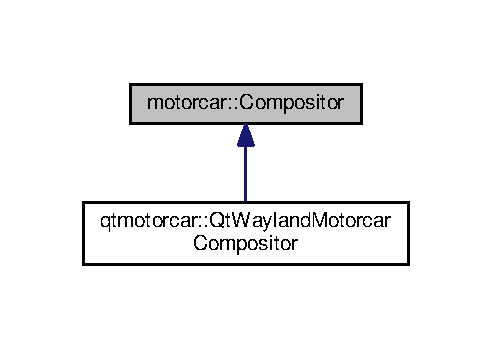
\includegraphics[width=254pt]{classmotorcar_1_1Compositor__inherit__graph}
\end{center}
\end{figure}


Collaboration diagram for motorcar\-:\-:Compositor\-:
\nopagebreak
\begin{figure}[H]
\begin{center}
\leavevmode
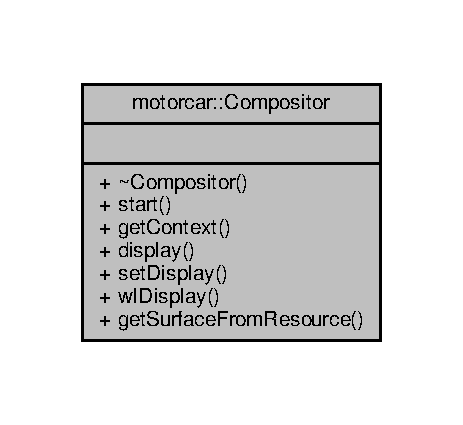
\includegraphics[width=190pt]{classmotorcar_1_1Compositor__coll__graph}
\end{center}
\end{figure}
\subsection*{Public Member Functions}
\begin{DoxyCompactItemize}
\item 
virtual \hyperlink{classmotorcar_1_1Compositor_ab9963bdfdd7deafdaec1a5ebf8f2d97b}{$\sim$\-Compositor} ()
\item 
virtual int \hyperlink{classmotorcar_1_1Compositor_a9d4b703e99386360996087a1100fae52}{start} ()=0
\item 
virtual \hyperlink{classmotorcar_1_1OpenGLContext}{Open\-G\-L\-Context} $\ast$ \hyperlink{classmotorcar_1_1Compositor_afb0a16529f65b5e2ecf8f15524680c57}{get\-Context} ()=0
\item 
\hyperlink{classmotorcar_1_1Display}{Display} $\ast$ \hyperlink{classmotorcar_1_1Compositor_a101830d8941b3d51a57e224950240cfe}{display} () const 
\item 
void \hyperlink{classmotorcar_1_1Compositor_a432fe3ad3e6ff3e22c61b3dc98f719f6}{set\-Display} (\hyperlink{classmotorcar_1_1Display}{Display} $\ast$\hyperlink{classmotorcar_1_1Compositor_a101830d8941b3d51a57e224950240cfe}{display})
\end{DoxyCompactItemize}


\subsection{Constructor \& Destructor Documentation}
\hypertarget{classmotorcar_1_1Compositor_ab9963bdfdd7deafdaec1a5ebf8f2d97b}{\index{motorcar\-::\-Compositor@{motorcar\-::\-Compositor}!$\sim$\-Compositor@{$\sim$\-Compositor}}
\index{$\sim$\-Compositor@{$\sim$\-Compositor}!motorcar::Compositor@{motorcar\-::\-Compositor}}
\subsubsection[{$\sim$\-Compositor}]{\setlength{\rightskip}{0pt plus 5cm}Compositor\-::$\sim$\-Compositor (
\begin{DoxyParamCaption}
{}
\end{DoxyParamCaption}
)\hspace{0.3cm}{\ttfamily [virtual]}}}\label{classmotorcar_1_1Compositor_ab9963bdfdd7deafdaec1a5ebf8f2d97b}


\subsection{Member Function Documentation}
\hypertarget{classmotorcar_1_1Compositor_a101830d8941b3d51a57e224950240cfe}{\index{motorcar\-::\-Compositor@{motorcar\-::\-Compositor}!display@{display}}
\index{display@{display}!motorcar::Compositor@{motorcar\-::\-Compositor}}
\subsubsection[{display}]{\setlength{\rightskip}{0pt plus 5cm}{\bf Display} $\ast$ Compositor\-::display (
\begin{DoxyParamCaption}
{}
\end{DoxyParamCaption}
) const}}\label{classmotorcar_1_1Compositor_a101830d8941b3d51a57e224950240cfe}
\hypertarget{classmotorcar_1_1Compositor_afb0a16529f65b5e2ecf8f15524680c57}{\index{motorcar\-::\-Compositor@{motorcar\-::\-Compositor}!get\-Context@{get\-Context}}
\index{get\-Context@{get\-Context}!motorcar::Compositor@{motorcar\-::\-Compositor}}
\subsubsection[{get\-Context}]{\setlength{\rightskip}{0pt plus 5cm}virtual {\bf Open\-G\-L\-Context}$\ast$ motorcar\-::\-Compositor\-::get\-Context (
\begin{DoxyParamCaption}
{}
\end{DoxyParamCaption}
)\hspace{0.3cm}{\ttfamily [pure virtual]}}}\label{classmotorcar_1_1Compositor_afb0a16529f65b5e2ecf8f15524680c57}


Implemented in \hyperlink{classqtmotorcar_1_1QtWaylandMotorcarCompositor_a1fb6e9d59011be2912bc9cf51496b191}{qtmotorcar\-::\-Qt\-Wayland\-Motorcar\-Compositor}.

\hypertarget{classmotorcar_1_1Compositor_a432fe3ad3e6ff3e22c61b3dc98f719f6}{\index{motorcar\-::\-Compositor@{motorcar\-::\-Compositor}!set\-Display@{set\-Display}}
\index{set\-Display@{set\-Display}!motorcar::Compositor@{motorcar\-::\-Compositor}}
\subsubsection[{set\-Display}]{\setlength{\rightskip}{0pt plus 5cm}void Compositor\-::set\-Display (
\begin{DoxyParamCaption}
\item[{{\bf Display} $\ast$}]{display}
\end{DoxyParamCaption}
)}}\label{classmotorcar_1_1Compositor_a432fe3ad3e6ff3e22c61b3dc98f719f6}
\hypertarget{classmotorcar_1_1Compositor_a9d4b703e99386360996087a1100fae52}{\index{motorcar\-::\-Compositor@{motorcar\-::\-Compositor}!start@{start}}
\index{start@{start}!motorcar::Compositor@{motorcar\-::\-Compositor}}
\subsubsection[{start}]{\setlength{\rightskip}{0pt plus 5cm}virtual int motorcar\-::\-Compositor\-::start (
\begin{DoxyParamCaption}
{}
\end{DoxyParamCaption}
)\hspace{0.3cm}{\ttfamily [pure virtual]}}}\label{classmotorcar_1_1Compositor_a9d4b703e99386360996087a1100fae52}


Implemented in \hyperlink{classqtmotorcar_1_1QtWaylandMotorcarCompositor_a34cd3f4acc535584eb066d3fe32ed9bf}{qtmotorcar\-::\-Qt\-Wayland\-Motorcar\-Compositor}.



The documentation for this class was generated from the following files\-:\begin{DoxyCompactItemize}
\item 
/home/dave/thesis/qtwayland-\/motorcar-\/compositor/motorcar/src/\hyperlink{compositor_8h}{compositor.\-h}\item 
/home/dave/thesis/qtwayland-\/motorcar-\/compositor/motorcar/src/\hyperlink{compositor_8cpp}{compositor.\-cpp}\end{DoxyCompactItemize}

\hypertarget{classmotorcar_1_1Display}{\section{motorcar\-:\-:Display Class Reference}
\label{classmotorcar_1_1Display}\index{motorcar\-::\-Display@{motorcar\-::\-Display}}
}


{\ttfamily \#include $<$display.\-h$>$}



Inheritance diagram for motorcar\-:\-:Display\-:
\nopagebreak
\begin{figure}[H]
\begin{center}
\leavevmode
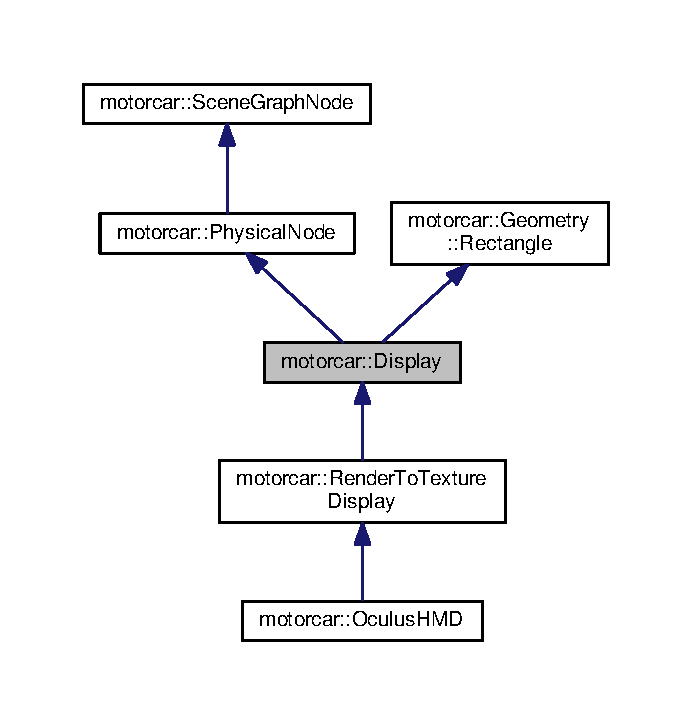
\includegraphics[width=332pt]{classmotorcar_1_1Display__inherit__graph}
\end{center}
\end{figure}


Collaboration diagram for motorcar\-:\-:Display\-:
\nopagebreak
\begin{figure}[H]
\begin{center}
\leavevmode
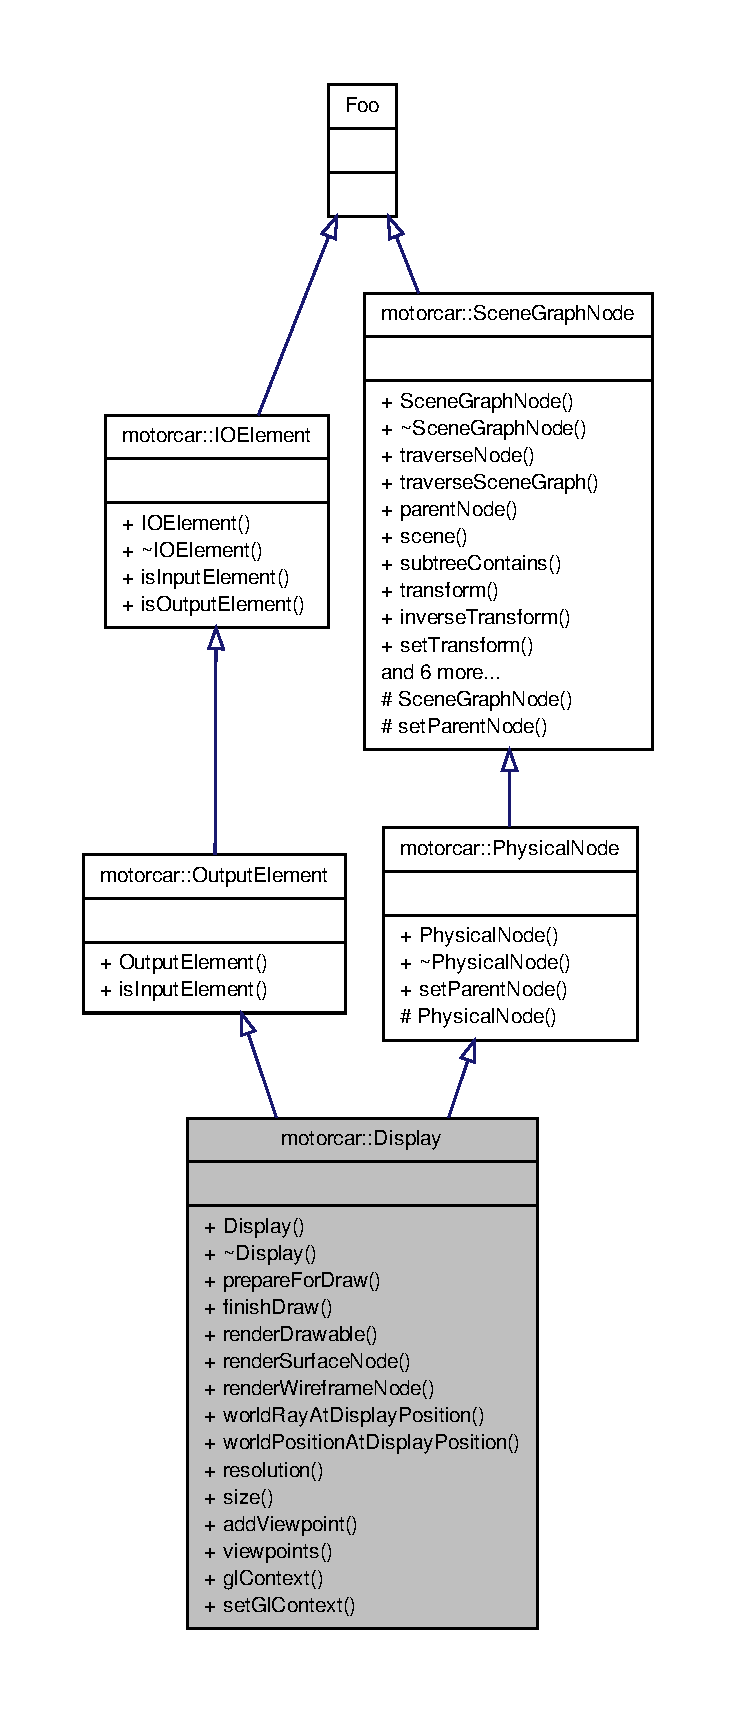
\includegraphics[width=332pt]{classmotorcar_1_1Display__coll__graph}
\end{center}
\end{figure}
\subsection*{Public Member Functions}
\begin{DoxyCompactItemize}
\item 
\hyperlink{classmotorcar_1_1Display_a2f7466d55b00caa97751ee242e0c633c}{Display} (\hyperlink{classmotorcar_1_1OpenGLContext}{Open\-G\-L\-Context} $\ast$\hyperlink{classmotorcar_1_1Display_a884dd0b78dbecee82a33eb6d26a2a403}{gl\-Context}, glm\-::vec2 display\-Dimensions, \hyperlink{classmotorcar_1_1PhysicalNode}{Physical\-Node} $\ast$parent, const glm\-::mat4 \&\hyperlink{classmotorcar_1_1SceneGraphNode_ad96e79fdd739ac8223a3128003be391a}{transform}=glm\-::mat4())
\item 
virtual \hyperlink{classmotorcar_1_1Display_ac2607a6bb236c55547a4223d40d85d1f}{$\sim$\-Display} ()
\item 
virtual void \hyperlink{classmotorcar_1_1Display_a0b26d9162f4f8f0848af408791be631c}{prepare\-For\-Draw} ()
\item 
virtual void \hyperlink{classmotorcar_1_1Display_a162b721d9c039887fc37b6a090ff1074}{finish\-Draw} ()
\item 
virtual \hyperlink{structmotorcar_1_1Geometry_1_1Ray}{Geometry\-::\-Ray} \hyperlink{classmotorcar_1_1Display_a9af842ec6ce47cdc901cb0310b0ef126}{world\-Ray\-At\-Display\-Position} (glm\-::vec2 pixel)
\item 
glm\-::vec3 \hyperlink{classmotorcar_1_1Display_ac3a8d4538e88df5b2bee043504620447}{world\-Position\-At\-Display\-Position} (glm\-::vec2 pixel)
\item 
virtual glm\-::ivec2 \hyperlink{classmotorcar_1_1Display_a58a94b72684d5b8569a9169591f7613e}{size} () override
\item 
virtual glm\-::vec2 \hyperlink{classmotorcar_1_1Display_aea90a885c5f3a124a3581bbeeeb4a425}{dimensions} () const 
\item 
void \hyperlink{classmotorcar_1_1Display_abd961f7f80a84ec143a81a159b07f0e8}{add\-Viewpoint} (\hyperlink{classmotorcar_1_1ViewPoint}{View\-Point} $\ast$v)
\item 
std\-::vector$<$ \hyperlink{classmotorcar_1_1ViewPoint}{View\-Point} $\ast$ $>$ \hyperlink{classmotorcar_1_1Display_acb3f10cbf366d80551f16e224e0bdf73}{viewpoints} () const 
\item 
\hyperlink{classmotorcar_1_1OpenGLContext}{Open\-G\-L\-Context} $\ast$ \hyperlink{classmotorcar_1_1Display_a884dd0b78dbecee82a33eb6d26a2a403}{gl\-Context} () const 
\item 
void \hyperlink{classmotorcar_1_1Display_a487018838d0ecfa96011a5ae5caa2e91}{set\-Gl\-Context} (\hyperlink{classmotorcar_1_1OpenGLContext}{Open\-G\-L\-Context} $\ast$\hyperlink{classmotorcar_1_1Display_a884dd0b78dbecee82a33eb6d26a2a403}{gl\-Context})
\item 
virtual G\-Luint \hyperlink{classmotorcar_1_1Display_a7318ea219f098a3a8b412dcec0745334}{active\-Frame\-Buffer} () const 
\item 
virtual G\-Luint \hyperlink{classmotorcar_1_1Display_a90c69af93ca9d9fff26839fce0e90d53}{depth\-Buffer\-Texture} () const 
\item 
G\-Luint \hyperlink{classmotorcar_1_1Display_ae3d75dd51cb2339bd06905635def61e3}{scratch\-Frame\-Buffer} () const 
\item 
G\-Luint \hyperlink{classmotorcar_1_1Display_a7feeb01b24470cacaee200fa944e24df}{scratch\-Color\-Buffer\-Texture} () const 
\item 
G\-Luint \hyperlink{classmotorcar_1_1Display_ad0b25afba9811f1e85bdf6e4fdc9ff74}{scratch\-Depth\-Buffer\-Texture} () const 
\end{DoxyCompactItemize}
\subsection*{Protected Attributes}
\begin{DoxyCompactItemize}
\item 
G\-Luint \hyperlink{classmotorcar_1_1Display_a23f2535f375102eda1ba2cba2b2a03a4}{m\-\_\-scratch\-Frame\-Buffer}
\item 
G\-Luint \hyperlink{classmotorcar_1_1Display_a8948636502d6498b53fbb644a9064390}{m\-\_\-scratch\-Color\-Buffer\-Texture}
\item 
G\-Luint \hyperlink{classmotorcar_1_1Display_a32e11a89219cf0727cd85b19a30f21a6}{m\-\_\-scratch\-Depth\-Buffer\-Texture}
\end{DoxyCompactItemize}
\subsection*{Additional Inherited Members}


\subsection{Constructor \& Destructor Documentation}
\hypertarget{classmotorcar_1_1Display_a2f7466d55b00caa97751ee242e0c633c}{\index{motorcar\-::\-Display@{motorcar\-::\-Display}!Display@{Display}}
\index{Display@{Display}!motorcar::Display@{motorcar\-::\-Display}}
\subsubsection[{Display}]{\setlength{\rightskip}{0pt plus 5cm}Display\-::\-Display (
\begin{DoxyParamCaption}
\item[{{\bf Open\-G\-L\-Context} $\ast$}]{gl\-Context, }
\item[{glm\-::vec2}]{display\-Dimensions, }
\item[{{\bf Physical\-Node} $\ast$}]{parent, }
\item[{const glm\-::mat4 \&}]{transform = {\ttfamily glm\-:\-:mat4()}}
\end{DoxyParamCaption}
)}}\label{classmotorcar_1_1Display_a2f7466d55b00caa97751ee242e0c633c}
\hypertarget{classmotorcar_1_1Display_ac2607a6bb236c55547a4223d40d85d1f}{\index{motorcar\-::\-Display@{motorcar\-::\-Display}!$\sim$\-Display@{$\sim$\-Display}}
\index{$\sim$\-Display@{$\sim$\-Display}!motorcar::Display@{motorcar\-::\-Display}}
\subsubsection[{$\sim$\-Display}]{\setlength{\rightskip}{0pt plus 5cm}Display\-::$\sim$\-Display (
\begin{DoxyParamCaption}
{}
\end{DoxyParamCaption}
)\hspace{0.3cm}{\ttfamily [virtual]}}}\label{classmotorcar_1_1Display_ac2607a6bb236c55547a4223d40d85d1f}


\subsection{Member Function Documentation}
\hypertarget{classmotorcar_1_1Display_a7318ea219f098a3a8b412dcec0745334}{\index{motorcar\-::\-Display@{motorcar\-::\-Display}!active\-Frame\-Buffer@{active\-Frame\-Buffer}}
\index{active\-Frame\-Buffer@{active\-Frame\-Buffer}!motorcar::Display@{motorcar\-::\-Display}}
\subsubsection[{active\-Frame\-Buffer}]{\setlength{\rightskip}{0pt plus 5cm}virtual G\-Luint motorcar\-::\-Display\-::active\-Frame\-Buffer (
\begin{DoxyParamCaption}
{}
\end{DoxyParamCaption}
) const\hspace{0.3cm}{\ttfamily [inline]}, {\ttfamily [virtual]}}}\label{classmotorcar_1_1Display_a7318ea219f098a3a8b412dcec0745334}


Reimplemented in \hyperlink{classmotorcar_1_1RenderToTextureDisplay_a8c928fb82c28d4785c58a1bd321e0ca6}{motorcar\-::\-Render\-To\-Texture\-Display}.

\hypertarget{classmotorcar_1_1Display_abd961f7f80a84ec143a81a159b07f0e8}{\index{motorcar\-::\-Display@{motorcar\-::\-Display}!add\-Viewpoint@{add\-Viewpoint}}
\index{add\-Viewpoint@{add\-Viewpoint}!motorcar::Display@{motorcar\-::\-Display}}
\subsubsection[{add\-Viewpoint}]{\setlength{\rightskip}{0pt plus 5cm}void Display\-::add\-Viewpoint (
\begin{DoxyParamCaption}
\item[{{\bf View\-Point} $\ast$}]{v}
\end{DoxyParamCaption}
)}}\label{classmotorcar_1_1Display_abd961f7f80a84ec143a81a159b07f0e8}
\hypertarget{classmotorcar_1_1Display_a90c69af93ca9d9fff26839fce0e90d53}{\index{motorcar\-::\-Display@{motorcar\-::\-Display}!depth\-Buffer\-Texture@{depth\-Buffer\-Texture}}
\index{depth\-Buffer\-Texture@{depth\-Buffer\-Texture}!motorcar::Display@{motorcar\-::\-Display}}
\subsubsection[{depth\-Buffer\-Texture}]{\setlength{\rightskip}{0pt plus 5cm}virtual G\-Luint motorcar\-::\-Display\-::depth\-Buffer\-Texture (
\begin{DoxyParamCaption}
{}
\end{DoxyParamCaption}
) const\hspace{0.3cm}{\ttfamily [inline]}, {\ttfamily [virtual]}}}\label{classmotorcar_1_1Display_a90c69af93ca9d9fff26839fce0e90d53}


Reimplemented in \hyperlink{classmotorcar_1_1RenderToTextureDisplay_a4dca5858105e2ee493ef0c49e62c37d4}{motorcar\-::\-Render\-To\-Texture\-Display}.

\hypertarget{classmotorcar_1_1Display_aea90a885c5f3a124a3581bbeeeb4a425}{\index{motorcar\-::\-Display@{motorcar\-::\-Display}!dimensions@{dimensions}}
\index{dimensions@{dimensions}!motorcar::Display@{motorcar\-::\-Display}}
\subsubsection[{dimensions}]{\setlength{\rightskip}{0pt plus 5cm}glm\-::vec2 Display\-::dimensions (
\begin{DoxyParamCaption}
{}
\end{DoxyParamCaption}
) const\hspace{0.3cm}{\ttfamily [virtual]}}}\label{classmotorcar_1_1Display_aea90a885c5f3a124a3581bbeeeb4a425}


Reimplemented in \hyperlink{classmotorcar_1_1RenderToTextureDisplay_a0ede4d9139786227f2c5d87bbbb9dcfa}{motorcar\-::\-Render\-To\-Texture\-Display}.

\hypertarget{classmotorcar_1_1Display_a162b721d9c039887fc37b6a090ff1074}{\index{motorcar\-::\-Display@{motorcar\-::\-Display}!finish\-Draw@{finish\-Draw}}
\index{finish\-Draw@{finish\-Draw}!motorcar::Display@{motorcar\-::\-Display}}
\subsubsection[{finish\-Draw}]{\setlength{\rightskip}{0pt plus 5cm}virtual void motorcar\-::\-Display\-::finish\-Draw (
\begin{DoxyParamCaption}
{}
\end{DoxyParamCaption}
)\hspace{0.3cm}{\ttfamily [inline]}, {\ttfamily [virtual]}}}\label{classmotorcar_1_1Display_a162b721d9c039887fc37b6a090ff1074}


Reimplemented in \hyperlink{classmotorcar_1_1RenderToTextureDisplay_a5a312b98ac49013155797e814e6cf69e}{motorcar\-::\-Render\-To\-Texture\-Display}.

\hypertarget{classmotorcar_1_1Display_a884dd0b78dbecee82a33eb6d26a2a403}{\index{motorcar\-::\-Display@{motorcar\-::\-Display}!gl\-Context@{gl\-Context}}
\index{gl\-Context@{gl\-Context}!motorcar::Display@{motorcar\-::\-Display}}
\subsubsection[{gl\-Context}]{\setlength{\rightskip}{0pt plus 5cm}{\bf Open\-G\-L\-Context} $\ast$ Display\-::gl\-Context (
\begin{DoxyParamCaption}
{}
\end{DoxyParamCaption}
) const}}\label{classmotorcar_1_1Display_a884dd0b78dbecee82a33eb6d26a2a403}
\hypertarget{classmotorcar_1_1Display_a0b26d9162f4f8f0848af408791be631c}{\index{motorcar\-::\-Display@{motorcar\-::\-Display}!prepare\-For\-Draw@{prepare\-For\-Draw}}
\index{prepare\-For\-Draw@{prepare\-For\-Draw}!motorcar::Display@{motorcar\-::\-Display}}
\subsubsection[{prepare\-For\-Draw}]{\setlength{\rightskip}{0pt plus 5cm}void Display\-::prepare\-For\-Draw (
\begin{DoxyParamCaption}
{}
\end{DoxyParamCaption}
)\hspace{0.3cm}{\ttfamily [virtual]}}}\label{classmotorcar_1_1Display_a0b26d9162f4f8f0848af408791be631c}


Reimplemented in \hyperlink{classmotorcar_1_1OculusHMD_ae9834ea50d728809532b7a48f7ed1738}{motorcar\-::\-Oculus\-H\-M\-D}, and \hyperlink{classmotorcar_1_1RenderToTextureDisplay_abdf6861fe69ada64fafd0a7713391bed}{motorcar\-::\-Render\-To\-Texture\-Display}.

\hypertarget{classmotorcar_1_1Display_a7feeb01b24470cacaee200fa944e24df}{\index{motorcar\-::\-Display@{motorcar\-::\-Display}!scratch\-Color\-Buffer\-Texture@{scratch\-Color\-Buffer\-Texture}}
\index{scratch\-Color\-Buffer\-Texture@{scratch\-Color\-Buffer\-Texture}!motorcar::Display@{motorcar\-::\-Display}}
\subsubsection[{scratch\-Color\-Buffer\-Texture}]{\setlength{\rightskip}{0pt plus 5cm}G\-Luint Display\-::scratch\-Color\-Buffer\-Texture (
\begin{DoxyParamCaption}
{}
\end{DoxyParamCaption}
) const}}\label{classmotorcar_1_1Display_a7feeb01b24470cacaee200fa944e24df}
\hypertarget{classmotorcar_1_1Display_ad0b25afba9811f1e85bdf6e4fdc9ff74}{\index{motorcar\-::\-Display@{motorcar\-::\-Display}!scratch\-Depth\-Buffer\-Texture@{scratch\-Depth\-Buffer\-Texture}}
\index{scratch\-Depth\-Buffer\-Texture@{scratch\-Depth\-Buffer\-Texture}!motorcar::Display@{motorcar\-::\-Display}}
\subsubsection[{scratch\-Depth\-Buffer\-Texture}]{\setlength{\rightskip}{0pt plus 5cm}G\-Luint Display\-::scratch\-Depth\-Buffer\-Texture (
\begin{DoxyParamCaption}
{}
\end{DoxyParamCaption}
) const}}\label{classmotorcar_1_1Display_ad0b25afba9811f1e85bdf6e4fdc9ff74}
\hypertarget{classmotorcar_1_1Display_ae3d75dd51cb2339bd06905635def61e3}{\index{motorcar\-::\-Display@{motorcar\-::\-Display}!scratch\-Frame\-Buffer@{scratch\-Frame\-Buffer}}
\index{scratch\-Frame\-Buffer@{scratch\-Frame\-Buffer}!motorcar::Display@{motorcar\-::\-Display}}
\subsubsection[{scratch\-Frame\-Buffer}]{\setlength{\rightskip}{0pt plus 5cm}G\-Luint Display\-::scratch\-Frame\-Buffer (
\begin{DoxyParamCaption}
{}
\end{DoxyParamCaption}
) const}}\label{classmotorcar_1_1Display_ae3d75dd51cb2339bd06905635def61e3}
\hypertarget{classmotorcar_1_1Display_a487018838d0ecfa96011a5ae5caa2e91}{\index{motorcar\-::\-Display@{motorcar\-::\-Display}!set\-Gl\-Context@{set\-Gl\-Context}}
\index{set\-Gl\-Context@{set\-Gl\-Context}!motorcar::Display@{motorcar\-::\-Display}}
\subsubsection[{set\-Gl\-Context}]{\setlength{\rightskip}{0pt plus 5cm}void Display\-::set\-Gl\-Context (
\begin{DoxyParamCaption}
\item[{{\bf Open\-G\-L\-Context} $\ast$}]{gl\-Context}
\end{DoxyParamCaption}
)}}\label{classmotorcar_1_1Display_a487018838d0ecfa96011a5ae5caa2e91}
\hypertarget{classmotorcar_1_1Display_a58a94b72684d5b8569a9169591f7613e}{\index{motorcar\-::\-Display@{motorcar\-::\-Display}!size@{size}}
\index{size@{size}!motorcar::Display@{motorcar\-::\-Display}}
\subsubsection[{size}]{\setlength{\rightskip}{0pt plus 5cm}glm\-::ivec2 Display\-::size (
\begin{DoxyParamCaption}
{}
\end{DoxyParamCaption}
)\hspace{0.3cm}{\ttfamily [override]}, {\ttfamily [virtual]}}}\label{classmotorcar_1_1Display_a58a94b72684d5b8569a9169591f7613e}


Reimplemented from \hyperlink{structmotorcar_1_1Geometry_1_1Rectangle_aef0385032dd32c2b2c762c08f1bfacf6}{motorcar\-::\-Geometry\-::\-Rectangle}.



Reimplemented in \hyperlink{classmotorcar_1_1RenderToTextureDisplay_a2e10611cf3fd629a4d962988642ad5b2}{motorcar\-::\-Render\-To\-Texture\-Display}.

\hypertarget{classmotorcar_1_1Display_acb3f10cbf366d80551f16e224e0bdf73}{\index{motorcar\-::\-Display@{motorcar\-::\-Display}!viewpoints@{viewpoints}}
\index{viewpoints@{viewpoints}!motorcar::Display@{motorcar\-::\-Display}}
\subsubsection[{viewpoints}]{\setlength{\rightskip}{0pt plus 5cm}std\-::vector$<$ {\bf View\-Point} $\ast$ $>$ Display\-::viewpoints (
\begin{DoxyParamCaption}
{}
\end{DoxyParamCaption}
) const}}\label{classmotorcar_1_1Display_acb3f10cbf366d80551f16e224e0bdf73}
\hypertarget{classmotorcar_1_1Display_ac3a8d4538e88df5b2bee043504620447}{\index{motorcar\-::\-Display@{motorcar\-::\-Display}!world\-Position\-At\-Display\-Position@{world\-Position\-At\-Display\-Position}}
\index{world\-Position\-At\-Display\-Position@{world\-Position\-At\-Display\-Position}!motorcar::Display@{motorcar\-::\-Display}}
\subsubsection[{world\-Position\-At\-Display\-Position}]{\setlength{\rightskip}{0pt plus 5cm}glm\-::vec3 Display\-::world\-Position\-At\-Display\-Position (
\begin{DoxyParamCaption}
\item[{glm\-::vec2}]{pixel}
\end{DoxyParamCaption}
)}}\label{classmotorcar_1_1Display_ac3a8d4538e88df5b2bee043504620447}
\hypertarget{classmotorcar_1_1Display_a9af842ec6ce47cdc901cb0310b0ef126}{\index{motorcar\-::\-Display@{motorcar\-::\-Display}!world\-Ray\-At\-Display\-Position@{world\-Ray\-At\-Display\-Position}}
\index{world\-Ray\-At\-Display\-Position@{world\-Ray\-At\-Display\-Position}!motorcar::Display@{motorcar\-::\-Display}}
\subsubsection[{world\-Ray\-At\-Display\-Position}]{\setlength{\rightskip}{0pt plus 5cm}{\bf Geometry\-::\-Ray} Display\-::world\-Ray\-At\-Display\-Position (
\begin{DoxyParamCaption}
\item[{glm\-::vec2}]{pixel}
\end{DoxyParamCaption}
)\hspace{0.3cm}{\ttfamily [virtual]}}}\label{classmotorcar_1_1Display_a9af842ec6ce47cdc901cb0310b0ef126}


\subsection{Member Data Documentation}
\hypertarget{classmotorcar_1_1Display_a8948636502d6498b53fbb644a9064390}{\index{motorcar\-::\-Display@{motorcar\-::\-Display}!m\-\_\-scratch\-Color\-Buffer\-Texture@{m\-\_\-scratch\-Color\-Buffer\-Texture}}
\index{m\-\_\-scratch\-Color\-Buffer\-Texture@{m\-\_\-scratch\-Color\-Buffer\-Texture}!motorcar::Display@{motorcar\-::\-Display}}
\subsubsection[{m\-\_\-scratch\-Color\-Buffer\-Texture}]{\setlength{\rightskip}{0pt plus 5cm}G\-Luint motorcar\-::\-Display\-::m\-\_\-scratch\-Color\-Buffer\-Texture\hspace{0.3cm}{\ttfamily [protected]}}}\label{classmotorcar_1_1Display_a8948636502d6498b53fbb644a9064390}
\hypertarget{classmotorcar_1_1Display_a32e11a89219cf0727cd85b19a30f21a6}{\index{motorcar\-::\-Display@{motorcar\-::\-Display}!m\-\_\-scratch\-Depth\-Buffer\-Texture@{m\-\_\-scratch\-Depth\-Buffer\-Texture}}
\index{m\-\_\-scratch\-Depth\-Buffer\-Texture@{m\-\_\-scratch\-Depth\-Buffer\-Texture}!motorcar::Display@{motorcar\-::\-Display}}
\subsubsection[{m\-\_\-scratch\-Depth\-Buffer\-Texture}]{\setlength{\rightskip}{0pt plus 5cm}G\-Luint motorcar\-::\-Display\-::m\-\_\-scratch\-Depth\-Buffer\-Texture\hspace{0.3cm}{\ttfamily [protected]}}}\label{classmotorcar_1_1Display_a32e11a89219cf0727cd85b19a30f21a6}
\hypertarget{classmotorcar_1_1Display_a23f2535f375102eda1ba2cba2b2a03a4}{\index{motorcar\-::\-Display@{motorcar\-::\-Display}!m\-\_\-scratch\-Frame\-Buffer@{m\-\_\-scratch\-Frame\-Buffer}}
\index{m\-\_\-scratch\-Frame\-Buffer@{m\-\_\-scratch\-Frame\-Buffer}!motorcar::Display@{motorcar\-::\-Display}}
\subsubsection[{m\-\_\-scratch\-Frame\-Buffer}]{\setlength{\rightskip}{0pt plus 5cm}G\-Luint motorcar\-::\-Display\-::m\-\_\-scratch\-Frame\-Buffer\hspace{0.3cm}{\ttfamily [protected]}}}\label{classmotorcar_1_1Display_a23f2535f375102eda1ba2cba2b2a03a4}


The documentation for this class was generated from the following files\-:\begin{DoxyCompactItemize}
\item 
/media/dave/e89b5eb4-\/4b10-\/4edf-\/8ad5-\/0d046a46b978/dave/thesis/qtwayland-\/motorcar-\/compositor/motorcar/src/scenegraph/output/display/\hyperlink{display_8h}{display.\-h}\item 
/media/dave/e89b5eb4-\/4b10-\/4edf-\/8ad5-\/0d046a46b978/dave/thesis/qtwayland-\/motorcar-\/compositor/motorcar/src/scenegraph/output/display/\hyperlink{display_8cpp}{display.\-cpp}\end{DoxyCompactItemize}

\hypertarget{classmotorcar_1_1Drawable}{\section{motorcar\-:\-:Drawable Class Reference}
\label{classmotorcar_1_1Drawable}\index{motorcar\-::\-Drawable@{motorcar\-::\-Drawable}}
}


{\ttfamily \#include $<$drawable.\-h$>$}



Inheritance diagram for motorcar\-:\-:Drawable\-:
\nopagebreak
\begin{figure}[H]
\begin{center}
\leavevmode
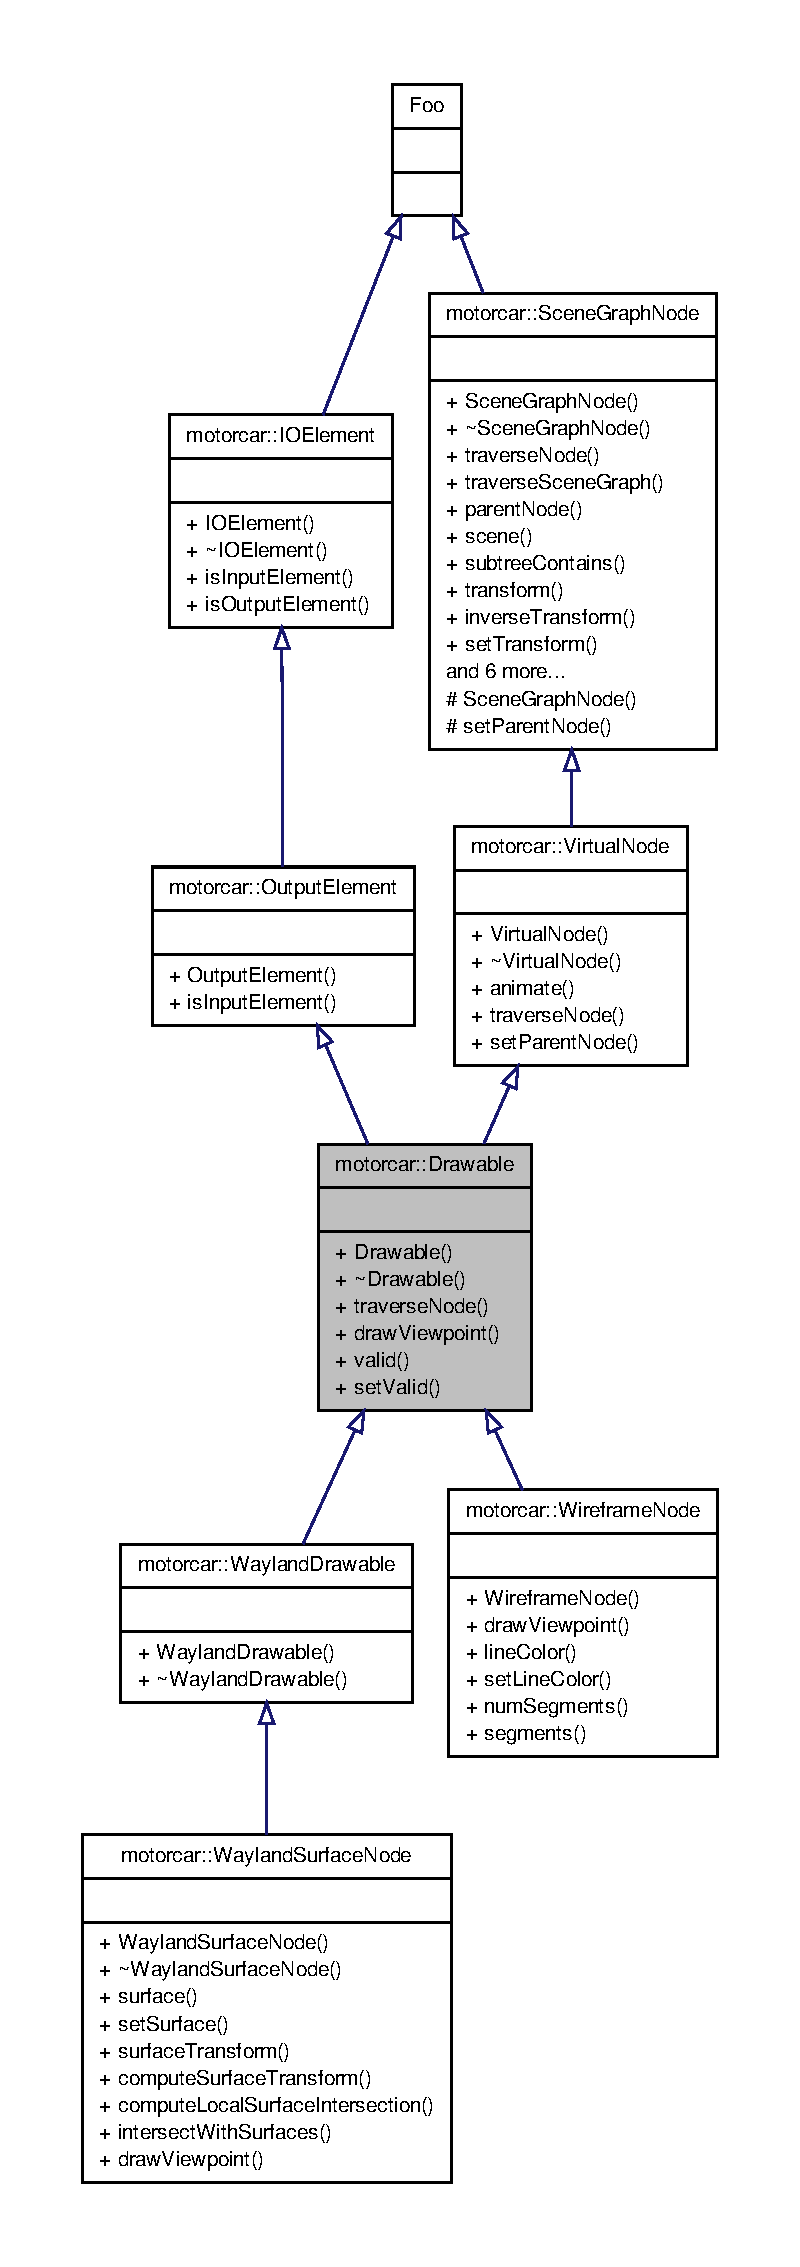
\includegraphics[width=350pt]{classmotorcar_1_1Drawable__inherit__graph}
\end{center}
\end{figure}


Collaboration diagram for motorcar\-:\-:Drawable\-:
\nopagebreak
\begin{figure}[H]
\begin{center}
\leavevmode
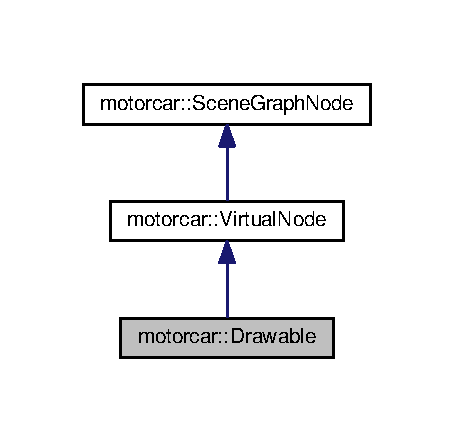
\includegraphics[width=218pt]{classmotorcar_1_1Drawable__coll__graph}
\end{center}
\end{figure}
\subsection*{Public Member Functions}
\begin{DoxyCompactItemize}
\item 
\hyperlink{classmotorcar_1_1Drawable_a48451c25ab7c1e379afec893f4c3d6f3}{Drawable} (\hyperlink{classmotorcar_1_1SceneGraphNode}{Scene\-Graph\-Node} $\ast$parent, const glm\-::mat4 \&\hyperlink{classmotorcar_1_1SceneGraphNode_ad96e79fdd739ac8223a3128003be391a}{transform}=glm\-::mat4())
\item 
virtual \hyperlink{classmotorcar_1_1Drawable_ab638464364b93a00bdeacc64cc85ba41}{$\sim$\-Drawable} ()
\item 
virtual void \hyperlink{classmotorcar_1_1Drawable_a8d0afa524298ae7f4ced15f6a80f253d}{draw} (\hyperlink{classmotorcar_1_1Scene}{Scene} $\ast$\hyperlink{classmotorcar_1_1SceneGraphNode_aa14e637ed4ae98f77e28941a4b5cfdd8}{scene}, \hyperlink{classmotorcar_1_1Display}{Display} $\ast$\hyperlink{structdisplay}{display})=0
\begin{DoxyCompactList}\small\item\em Draw this node for the current display. \end{DoxyCompactList}\item 
virtual void \hyperlink{classmotorcar_1_1Drawable_a8dce7e2370f9fdc5394cf661effc865a}{handle\-Frame\-Draw} (\hyperlink{classmotorcar_1_1Scene}{Scene} $\ast$\hyperlink{classmotorcar_1_1SceneGraphNode_aa14e637ed4ae98f77e28941a4b5cfdd8}{scene}) override
\begin{DoxyCompactList}\small\item\em Gets the active display from the scene and calls draw on it. \end{DoxyCompactList}\item 
bool \hyperlink{classmotorcar_1_1Drawable_ae76952e4af87589dbb7a4c9f17f2fdfa}{visible} () const 
\item 
void \hyperlink{classmotorcar_1_1Drawable_a3aa8dfd1f526d0cf744313e8e102cea4}{set\-Visible} (bool \hyperlink{classmotorcar_1_1Drawable_ae76952e4af87589dbb7a4c9f17f2fdfa}{visible})
\end{DoxyCompactItemize}
\subsection*{Additional Inherited Members}


\subsection{Constructor \& Destructor Documentation}
\hypertarget{classmotorcar_1_1Drawable_a48451c25ab7c1e379afec893f4c3d6f3}{\index{motorcar\-::\-Drawable@{motorcar\-::\-Drawable}!Drawable@{Drawable}}
\index{Drawable@{Drawable}!motorcar::Drawable@{motorcar\-::\-Drawable}}
\subsubsection[{Drawable}]{\setlength{\rightskip}{0pt plus 5cm}Drawable\-::\-Drawable (
\begin{DoxyParamCaption}
\item[{{\bf Scene\-Graph\-Node} $\ast$}]{parent, }
\item[{const glm\-::mat4 \&}]{transform = {\ttfamily glm\-:\-:mat4()}}
\end{DoxyParamCaption}
)}}\label{classmotorcar_1_1Drawable_a48451c25ab7c1e379afec893f4c3d6f3}
\hypertarget{classmotorcar_1_1Drawable_ab638464364b93a00bdeacc64cc85ba41}{\index{motorcar\-::\-Drawable@{motorcar\-::\-Drawable}!$\sim$\-Drawable@{$\sim$\-Drawable}}
\index{$\sim$\-Drawable@{$\sim$\-Drawable}!motorcar::Drawable@{motorcar\-::\-Drawable}}
\subsubsection[{$\sim$\-Drawable}]{\setlength{\rightskip}{0pt plus 5cm}virtual motorcar\-::\-Drawable\-::$\sim$\-Drawable (
\begin{DoxyParamCaption}
{}
\end{DoxyParamCaption}
)\hspace{0.3cm}{\ttfamily [inline]}, {\ttfamily [virtual]}}}\label{classmotorcar_1_1Drawable_ab638464364b93a00bdeacc64cc85ba41}


\subsection{Member Function Documentation}
\hypertarget{classmotorcar_1_1Drawable_a8d0afa524298ae7f4ced15f6a80f253d}{\index{motorcar\-::\-Drawable@{motorcar\-::\-Drawable}!draw@{draw}}
\index{draw@{draw}!motorcar::Drawable@{motorcar\-::\-Drawable}}
\subsubsection[{draw}]{\setlength{\rightskip}{0pt plus 5cm}virtual void motorcar\-::\-Drawable\-::draw (
\begin{DoxyParamCaption}
\item[{{\bf Scene} $\ast$}]{scene, }
\item[{{\bf Display} $\ast$}]{display}
\end{DoxyParamCaption}
)\hspace{0.3cm}{\ttfamily [pure virtual]}}}\label{classmotorcar_1_1Drawable_a8d0afa524298ae7f4ced15f6a80f253d}


Draw this node for the current display. 



Implemented in \hyperlink{classmotorcar_1_1WaylandSurfaceNode_a1afe3178777574dd1b3c66d7d19d871b}{motorcar\-::\-Wayland\-Surface\-Node}, \hyperlink{classmotorcar_1_1SoftKineticDepthCamera_a2752b6bf323e019a4cec43b61d78bcff}{motorcar\-::\-Soft\-Kinetic\-Depth\-Camera}, \hyperlink{classmotorcar_1_1DepthCompositedSurfaceNode_a2108d586ac8641beec9f6d048e3ea562}{motorcar\-::\-Depth\-Composited\-Surface\-Node}, and \hyperlink{classmotorcar_1_1WireframeNode_a8be77469b6c99cfb05c2096b6d064c2e}{motorcar\-::\-Wireframe\-Node}.

\hypertarget{classmotorcar_1_1Drawable_a8dce7e2370f9fdc5394cf661effc865a}{\index{motorcar\-::\-Drawable@{motorcar\-::\-Drawable}!handle\-Frame\-Draw@{handle\-Frame\-Draw}}
\index{handle\-Frame\-Draw@{handle\-Frame\-Draw}!motorcar::Drawable@{motorcar\-::\-Drawable}}
\subsubsection[{handle\-Frame\-Draw}]{\setlength{\rightskip}{0pt plus 5cm}void Drawable\-::handle\-Frame\-Draw (
\begin{DoxyParamCaption}
\item[{{\bf Scene} $\ast$}]{scene}
\end{DoxyParamCaption}
)\hspace{0.3cm}{\ttfamily [override]}, {\ttfamily [virtual]}}}\label{classmotorcar_1_1Drawable_a8dce7e2370f9fdc5394cf661effc865a}


Gets the active display from the scene and calls draw on it. 



Reimplemented from \hyperlink{classmotorcar_1_1SceneGraphNode_a06f85abeee71ebe2b21ca9d6d20d7e67}{motorcar\-::\-Scene\-Graph\-Node}.

\hypertarget{classmotorcar_1_1Drawable_a3aa8dfd1f526d0cf744313e8e102cea4}{\index{motorcar\-::\-Drawable@{motorcar\-::\-Drawable}!set\-Visible@{set\-Visible}}
\index{set\-Visible@{set\-Visible}!motorcar::Drawable@{motorcar\-::\-Drawable}}
\subsubsection[{set\-Visible}]{\setlength{\rightskip}{0pt plus 5cm}void Drawable\-::set\-Visible (
\begin{DoxyParamCaption}
\item[{bool}]{visible}
\end{DoxyParamCaption}
)}}\label{classmotorcar_1_1Drawable_a3aa8dfd1f526d0cf744313e8e102cea4}
\hypertarget{classmotorcar_1_1Drawable_ae76952e4af87589dbb7a4c9f17f2fdfa}{\index{motorcar\-::\-Drawable@{motorcar\-::\-Drawable}!visible@{visible}}
\index{visible@{visible}!motorcar::Drawable@{motorcar\-::\-Drawable}}
\subsubsection[{visible}]{\setlength{\rightskip}{0pt plus 5cm}bool Drawable\-::visible (
\begin{DoxyParamCaption}
{}
\end{DoxyParamCaption}
) const}}\label{classmotorcar_1_1Drawable_ae76952e4af87589dbb7a4c9f17f2fdfa}


The documentation for this class was generated from the following files\-:\begin{DoxyCompactItemize}
\item 
/media/dave/e89b5eb4-\/4b10-\/4edf-\/8ad5-\/0d046a46b978/dave/thesis/qtwayland-\/motorcar-\/compositor/motorcar/src/scenegraph/output/\hyperlink{drawable_8h}{drawable.\-h}\item 
/media/dave/e89b5eb4-\/4b10-\/4edf-\/8ad5-\/0d046a46b978/dave/thesis/qtwayland-\/motorcar-\/compositor/motorcar/src/scenegraph/output/\hyperlink{drawable_8cpp}{drawable.\-cpp}\end{DoxyCompactItemize}

\hypertarget{classFoo}{\section{Foo Class Reference}
\label{classFoo}\index{Foo@{Foo}}
}


{\ttfamily \#include $<$foo.\-h$>$}



Inheritance diagram for Foo\-:
\nopagebreak
\begin{figure}[H]
\begin{center}
\leavevmode
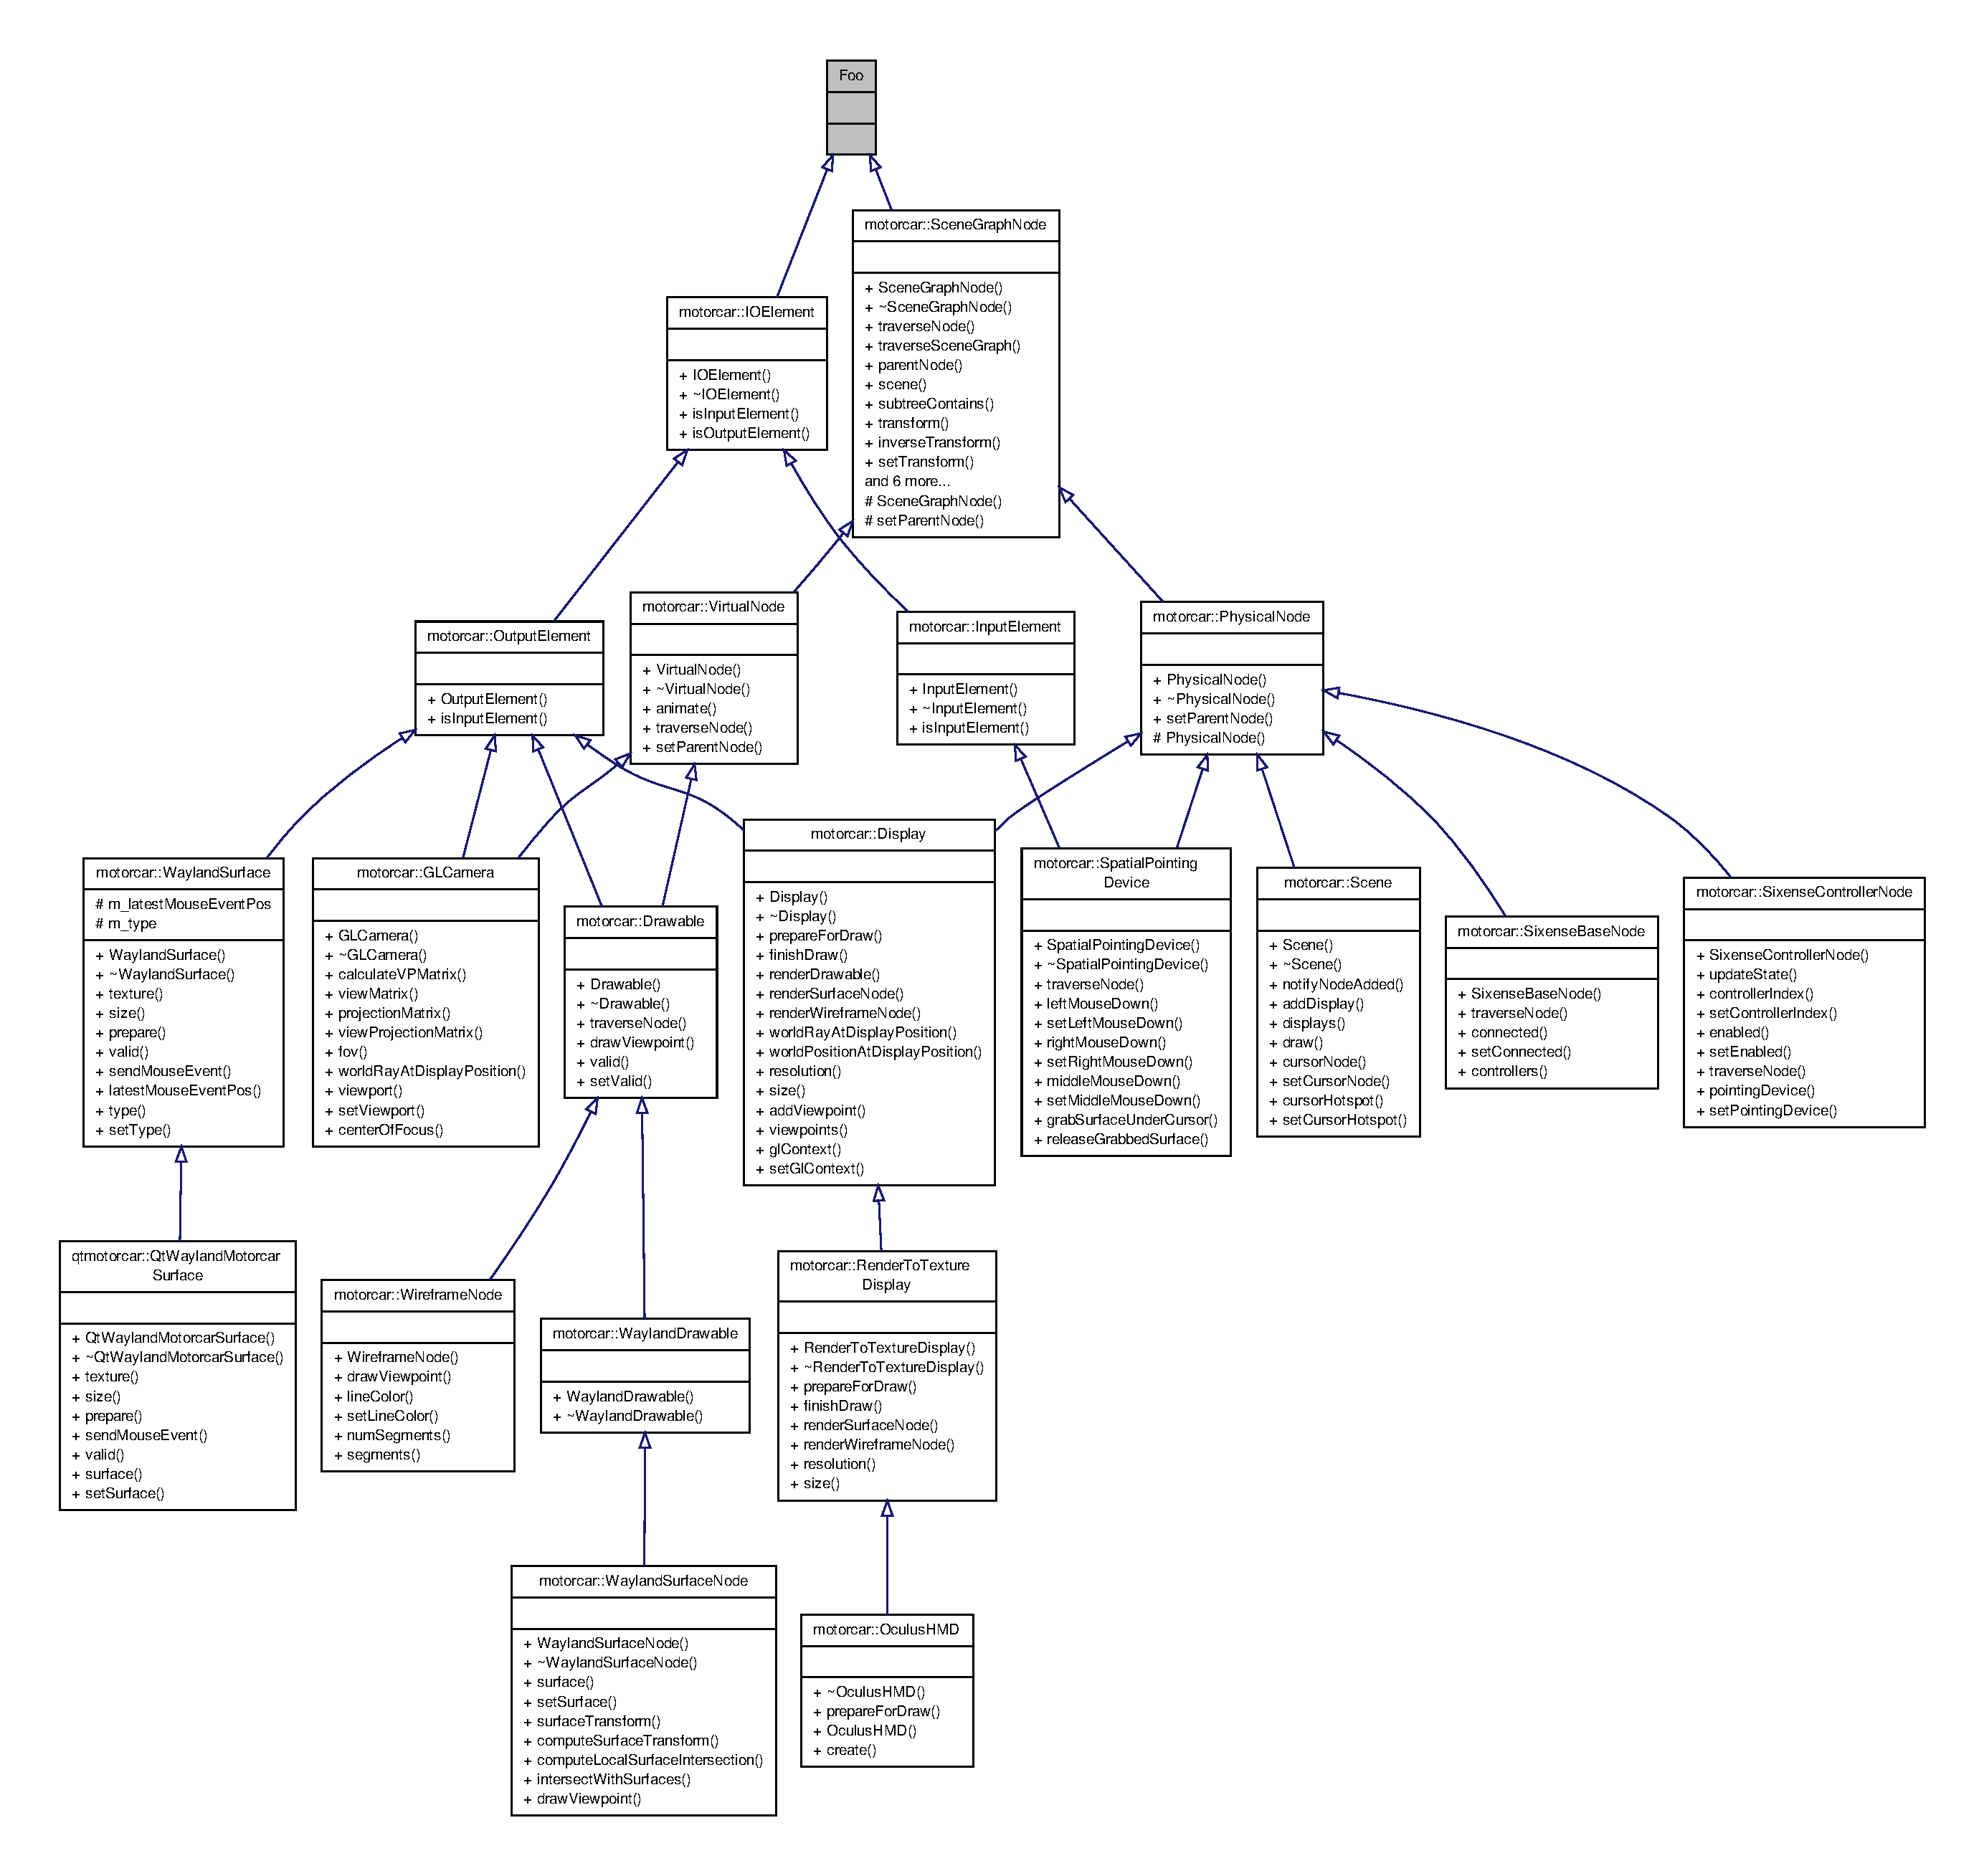
\includegraphics[width=350pt]{classFoo__inherit__graph}
\end{center}
\end{figure}


Collaboration diagram for Foo\-:
\nopagebreak
\begin{figure}[H]
\begin{center}
\leavevmode
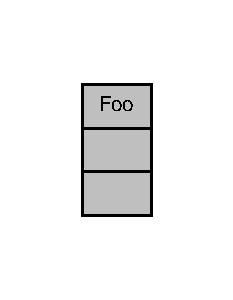
\includegraphics[width=112pt]{classFoo__coll__graph}
\end{center}
\end{figure}


The documentation for this class was generated from the following file\-:\begin{DoxyCompactItemize}
\item 
/home/dave/thesis/qtwayland-\/motorcar-\/compositor/motorcar/src/scenegraph/\hyperlink{foo_8h}{foo.\-h}\end{DoxyCompactItemize}

\hypertarget{classmotorcar_1_1Geometry}{\section{motorcar\-:\-:Geometry Class Reference}
\label{classmotorcar_1_1Geometry}\index{motorcar\-::\-Geometry@{motorcar\-::\-Geometry}}
}


{\ttfamily \#include $<$geometry.\-h$>$}

\subsection*{Classes}
\begin{DoxyCompactItemize}
\item 
struct \hyperlink{structmotorcar_1_1Geometry_1_1AxisAlignedBox}{Axis\-Aligned\-Box}
\item 
struct \hyperlink{structmotorcar_1_1Geometry_1_1Plane}{Plane}
\item 
struct \hyperlink{structmotorcar_1_1Geometry_1_1Ray}{Ray}
\item 
struct \hyperlink{structmotorcar_1_1Geometry_1_1RaySurfaceIntersection}{Ray\-Surface\-Intersection}
\item 
struct \hyperlink{structmotorcar_1_1Geometry_1_1Rectangle}{Rectangle}
\end{DoxyCompactItemize}
\subsection*{Static Public Member Functions}
\begin{DoxyCompactItemize}
\item 
static void \hyperlink{classmotorcar_1_1Geometry_a35ee70e5dab9981b9f1914eca9580b06}{print\-Matrix} (glm\-::mat4 m)
\item 
static void \hyperlink{classmotorcar_1_1Geometry_a97660333acd464a86c5ab7f5672fb3d2}{print\-Vector} (glm\-::vec3 v)
\end{DoxyCompactItemize}


\subsection{Member Function Documentation}
\hypertarget{classmotorcar_1_1Geometry_a35ee70e5dab9981b9f1914eca9580b06}{\index{motorcar\-::\-Geometry@{motorcar\-::\-Geometry}!print\-Matrix@{print\-Matrix}}
\index{print\-Matrix@{print\-Matrix}!motorcar::Geometry@{motorcar\-::\-Geometry}}
\subsubsection[{print\-Matrix}]{\setlength{\rightskip}{0pt plus 5cm}void Geometry\-::print\-Matrix (
\begin{DoxyParamCaption}
\item[{glm\-::mat4}]{m}
\end{DoxyParamCaption}
)\hspace{0.3cm}{\ttfamily [static]}}}\label{classmotorcar_1_1Geometry_a35ee70e5dab9981b9f1914eca9580b06}
\hypertarget{classmotorcar_1_1Geometry_a97660333acd464a86c5ab7f5672fb3d2}{\index{motorcar\-::\-Geometry@{motorcar\-::\-Geometry}!print\-Vector@{print\-Vector}}
\index{print\-Vector@{print\-Vector}!motorcar::Geometry@{motorcar\-::\-Geometry}}
\subsubsection[{print\-Vector}]{\setlength{\rightskip}{0pt plus 5cm}void Geometry\-::print\-Vector (
\begin{DoxyParamCaption}
\item[{glm\-::vec3}]{v}
\end{DoxyParamCaption}
)\hspace{0.3cm}{\ttfamily [static]}}}\label{classmotorcar_1_1Geometry_a97660333acd464a86c5ab7f5672fb3d2}


The documentation for this class was generated from the following files\-:\begin{DoxyCompactItemize}
\item 
/home/dave/thesis/motorcar/src/compositor/\hyperlink{geometry_8h}{geometry.\-h}\item 
/home/dave/thesis/motorcar/src/compositor/\hyperlink{geometry_8cpp}{geometry.\-cpp}\end{DoxyCompactItemize}

\hypertarget{classGlBufferObject}{\section{Gl\-Buffer\-Object Class Reference}
\label{classGlBufferObject}\index{Gl\-Buffer\-Object@{Gl\-Buffer\-Object}}
}


{\ttfamily \#include $<$G\-L\-S\-L\-Helper.\-h$>$}

\subsection*{Public Member Functions}
\begin{DoxyCompactItemize}
\item 
\hyperlink{classGlBufferObject_a5346228ff9f5b1c806a9d03ece525dbb}{Gl\-Buffer\-Object} ()
\item 
\hyperlink{classGlBufferObject_a046d6e2874c10d04aa16e4846b1e93d7}{$\sim$\-Gl\-Buffer\-Object} ()
\item 
\hyperlink{classGlBufferObject_a0f71903669c77f142202c62b897a5c00}{operator G\-Luint} () const 
\end{DoxyCompactItemize}


\subsection{Constructor \& Destructor Documentation}
\hypertarget{classGlBufferObject_a5346228ff9f5b1c806a9d03ece525dbb}{\index{Gl\-Buffer\-Object@{Gl\-Buffer\-Object}!Gl\-Buffer\-Object@{Gl\-Buffer\-Object}}
\index{Gl\-Buffer\-Object@{Gl\-Buffer\-Object}!GlBufferObject@{Gl\-Buffer\-Object}}
\subsubsection[{Gl\-Buffer\-Object}]{\setlength{\rightskip}{0pt plus 5cm}Gl\-Buffer\-Object\-::\-Gl\-Buffer\-Object (
\begin{DoxyParamCaption}
{}
\end{DoxyParamCaption}
)\hspace{0.3cm}{\ttfamily [inline]}}}\label{classGlBufferObject_a5346228ff9f5b1c806a9d03ece525dbb}
\hypertarget{classGlBufferObject_a046d6e2874c10d04aa16e4846b1e93d7}{\index{Gl\-Buffer\-Object@{Gl\-Buffer\-Object}!$\sim$\-Gl\-Buffer\-Object@{$\sim$\-Gl\-Buffer\-Object}}
\index{$\sim$\-Gl\-Buffer\-Object@{$\sim$\-Gl\-Buffer\-Object}!GlBufferObject@{Gl\-Buffer\-Object}}
\subsubsection[{$\sim$\-Gl\-Buffer\-Object}]{\setlength{\rightskip}{0pt plus 5cm}Gl\-Buffer\-Object\-::$\sim$\-Gl\-Buffer\-Object (
\begin{DoxyParamCaption}
{}
\end{DoxyParamCaption}
)\hspace{0.3cm}{\ttfamily [inline]}}}\label{classGlBufferObject_a046d6e2874c10d04aa16e4846b1e93d7}


\subsection{Member Function Documentation}
\hypertarget{classGlBufferObject_a0f71903669c77f142202c62b897a5c00}{\index{Gl\-Buffer\-Object@{Gl\-Buffer\-Object}!operator G\-Luint@{operator G\-Luint}}
\index{operator G\-Luint@{operator G\-Luint}!GlBufferObject@{Gl\-Buffer\-Object}}
\subsubsection[{operator G\-Luint}]{\setlength{\rightskip}{0pt plus 5cm}Gl\-Buffer\-Object\-::operator G\-Luint (
\begin{DoxyParamCaption}
{}
\end{DoxyParamCaption}
) const\hspace{0.3cm}{\ttfamily [inline]}}}\label{classGlBufferObject_a0f71903669c77f142202c62b897a5c00}


The documentation for this class was generated from the following file\-:\begin{DoxyCompactItemize}
\item 
/media/dave/e89b5eb4-\/4b10-\/4edf-\/8ad5-\/0d046a46b978/dave/thesis/qtwayland-\/motorcar-\/compositor/motorcar/src/gl/\hyperlink{GLSLHelper_8h}{G\-L\-S\-L\-Helper.\-h}\end{DoxyCompactItemize}

\hypertarget{classmotorcar_1_1GLCamera}{\section{motorcar\-:\-:G\-L\-Camera Class Reference}
\label{classmotorcar_1_1GLCamera}\index{motorcar\-::\-G\-L\-Camera@{motorcar\-::\-G\-L\-Camera}}
}


{\ttfamily \#include $<$glcameranode.\-h$>$}



Inheritance diagram for motorcar\-:\-:G\-L\-Camera\-:
\nopagebreak
\begin{figure}[H]
\begin{center}
\leavevmode
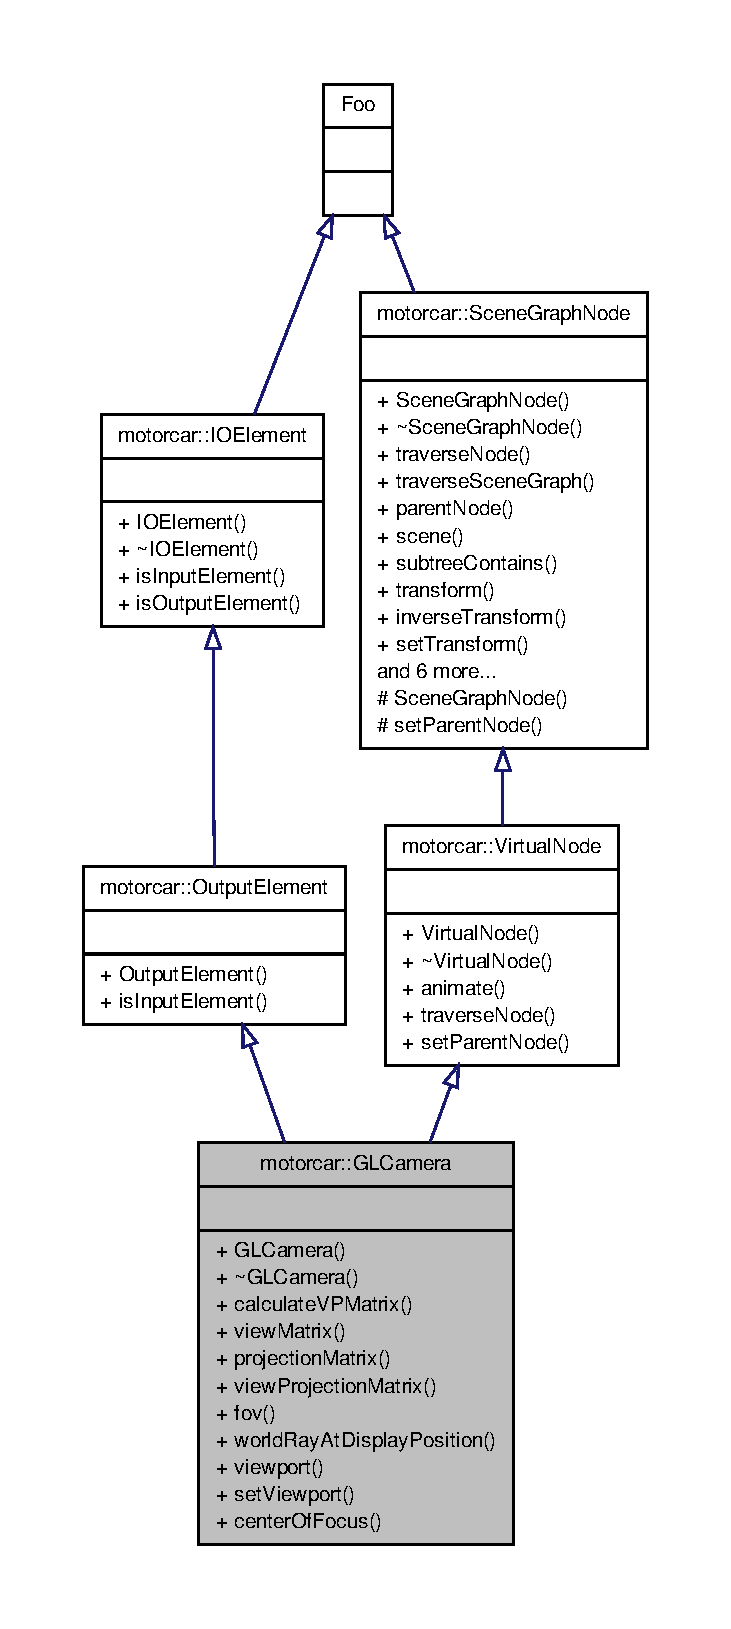
\includegraphics[height=550pt]{classmotorcar_1_1GLCamera__inherit__graph}
\end{center}
\end{figure}


Collaboration diagram for motorcar\-:\-:G\-L\-Camera\-:
\nopagebreak
\begin{figure}[H]
\begin{center}
\leavevmode
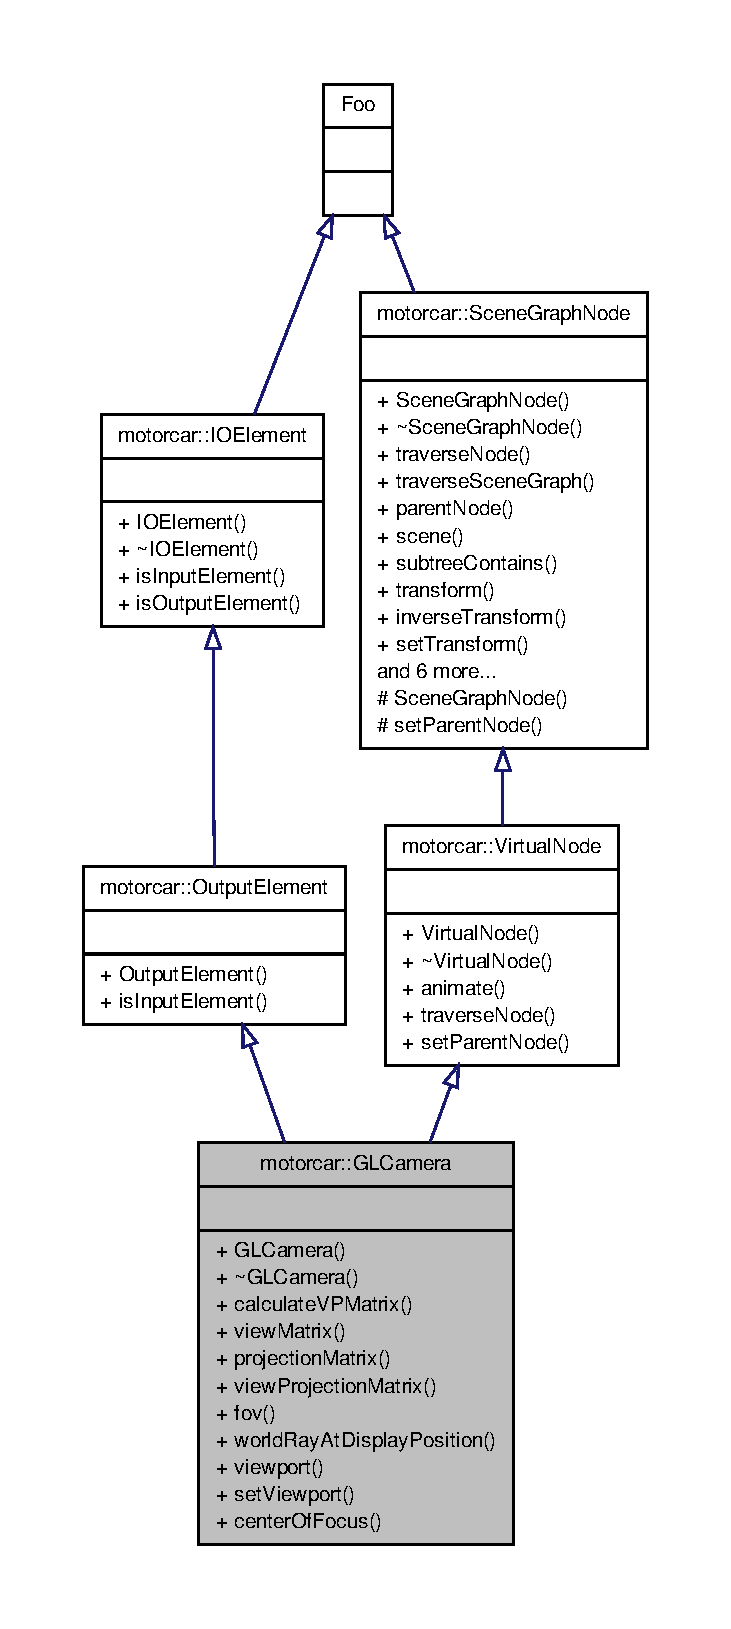
\includegraphics[height=550pt]{classmotorcar_1_1GLCamera__coll__graph}
\end{center}
\end{figure}
\subsection*{Classes}
\begin{DoxyCompactItemize}
\item 
class \hyperlink{classmotorcar_1_1GLCamera_1_1GLViewPort}{G\-L\-View\-Port}
\end{DoxyCompactItemize}
\subsection*{Public Member Functions}
\begin{DoxyCompactItemize}
\item 
\hyperlink{classmotorcar_1_1GLCamera_aaaf4065034f1f9a9a430c9f8e73d0708}{G\-L\-Camera} (float near, float far, \hyperlink{classmotorcar_1_1Display}{Display} $\ast$display, \hyperlink{classmotorcar_1_1SceneGraphNode}{Scene\-Graph\-Node} $\ast$parent, glm\-::mat4 \hyperlink{classmotorcar_1_1SceneGraphNode_ad96e79fdd739ac8223a3128003be391a}{transform}=glm\-::mat4(), glm\-::vec4 view\-Port\-Params=glm\-::vec4(0, 0, 1, 1), glm\-::vec3 center\-Of\-Projection=glm\-::vec3(0))
\item 
\hyperlink{classmotorcar_1_1GLCamera_a0622c29828396fc68be023b8c871e401}{$\sim$\-G\-L\-Camera} ()
\item 
void \hyperlink{classmotorcar_1_1GLCamera_a8f223614a636b9a9385d9acf2b8151f6}{calculate\-V\-P\-Matrix} ()
\item 
glm\-::mat4 \hyperlink{classmotorcar_1_1GLCamera_afd59fa3adac82a28eb786f2b70a6dbfa}{view\-Matrix} () const 
\item 
glm\-::mat4 \hyperlink{classmotorcar_1_1GLCamera_ab9391c9d7d91ea2b0a05a3881dc368c8}{projection\-Matrix} () const 
\item 
glm\-::mat4 \hyperlink{classmotorcar_1_1GLCamera_a8c737d347500a9a8aa5866098be545a4}{view\-Projection\-Matrix} () const 
\item 
float \hyperlink{classmotorcar_1_1GLCamera_a108d5a76c7855b25d8f93185e911b154}{fov} ()
\item 
\hyperlink{structmotorcar_1_1Geometry_1_1Ray}{Geometry\-::\-Ray} \hyperlink{classmotorcar_1_1GLCamera_a3253b3f3cb2e88b6e17c48744ea44766}{world\-Ray\-At\-Display\-Position} (float pixel\-X, float pixel\-Y)
\item 
\hyperlink{classmotorcar_1_1GLCamera_1_1GLViewPort}{G\-L\-View\-Port} $\ast$ \hyperlink{classmotorcar_1_1GLCamera_ab31d52c7ae376ef06f00d924461b7820}{viewport} () const 
\item 
void \hyperlink{classmotorcar_1_1GLCamera_ad3d5b539a4f8565c0c1cde9f00b4074c}{set\-Viewport} (\hyperlink{classmotorcar_1_1GLCamera_1_1GLViewPort}{G\-L\-View\-Port} $\ast$\hyperlink{classmotorcar_1_1GLCamera_ab31d52c7ae376ef06f00d924461b7820}{viewport})
\item 
glm\-::vec4 \hyperlink{classmotorcar_1_1GLCamera_a55aec53065d06faff1466aff35c20cdb}{center\-Of\-Focus} () const 
\end{DoxyCompactItemize}
\subsection*{Additional Inherited Members}


\subsection{Constructor \& Destructor Documentation}
\hypertarget{classmotorcar_1_1GLCamera_aaaf4065034f1f9a9a430c9f8e73d0708}{\index{motorcar\-::\-G\-L\-Camera@{motorcar\-::\-G\-L\-Camera}!G\-L\-Camera@{G\-L\-Camera}}
\index{G\-L\-Camera@{G\-L\-Camera}!motorcar::GLCamera@{motorcar\-::\-G\-L\-Camera}}
\subsubsection[{G\-L\-Camera}]{\setlength{\rightskip}{0pt plus 5cm}G\-L\-Camera\-::\-G\-L\-Camera (
\begin{DoxyParamCaption}
\item[{float}]{near, }
\item[{float}]{far, }
\item[{{\bf Display} $\ast$}]{display, }
\item[{{\bf Scene\-Graph\-Node} $\ast$}]{parent, }
\item[{glm\-::mat4}]{transform = {\ttfamily glm\-:\-:mat4()}, }
\item[{glm\-::vec4}]{view\-Port\-Params = {\ttfamily glm\-:\-:vec4(0,0,1,1)}, }
\item[{glm\-::vec3}]{center\-Of\-Projection = {\ttfamily glm\-:\-:vec3(0)}}
\end{DoxyParamCaption}
)}}\label{classmotorcar_1_1GLCamera_aaaf4065034f1f9a9a430c9f8e73d0708}
\hypertarget{classmotorcar_1_1GLCamera_a0622c29828396fc68be023b8c871e401}{\index{motorcar\-::\-G\-L\-Camera@{motorcar\-::\-G\-L\-Camera}!$\sim$\-G\-L\-Camera@{$\sim$\-G\-L\-Camera}}
\index{$\sim$\-G\-L\-Camera@{$\sim$\-G\-L\-Camera}!motorcar::GLCamera@{motorcar\-::\-G\-L\-Camera}}
\subsubsection[{$\sim$\-G\-L\-Camera}]{\setlength{\rightskip}{0pt plus 5cm}G\-L\-Camera\-::$\sim$\-G\-L\-Camera (
\begin{DoxyParamCaption}
{}
\end{DoxyParamCaption}
)}}\label{classmotorcar_1_1GLCamera_a0622c29828396fc68be023b8c871e401}


\subsection{Member Function Documentation}
\hypertarget{classmotorcar_1_1GLCamera_a8f223614a636b9a9385d9acf2b8151f6}{\index{motorcar\-::\-G\-L\-Camera@{motorcar\-::\-G\-L\-Camera}!calculate\-V\-P\-Matrix@{calculate\-V\-P\-Matrix}}
\index{calculate\-V\-P\-Matrix@{calculate\-V\-P\-Matrix}!motorcar::GLCamera@{motorcar\-::\-G\-L\-Camera}}
\subsubsection[{calculate\-V\-P\-Matrix}]{\setlength{\rightskip}{0pt plus 5cm}void G\-L\-Camera\-::calculate\-V\-P\-Matrix (
\begin{DoxyParamCaption}
{}
\end{DoxyParamCaption}
)}}\label{classmotorcar_1_1GLCamera_a8f223614a636b9a9385d9acf2b8151f6}
\hypertarget{classmotorcar_1_1GLCamera_a55aec53065d06faff1466aff35c20cdb}{\index{motorcar\-::\-G\-L\-Camera@{motorcar\-::\-G\-L\-Camera}!center\-Of\-Focus@{center\-Of\-Focus}}
\index{center\-Of\-Focus@{center\-Of\-Focus}!motorcar::GLCamera@{motorcar\-::\-G\-L\-Camera}}
\subsubsection[{center\-Of\-Focus}]{\setlength{\rightskip}{0pt plus 5cm}glm\-::vec4 G\-L\-Camera\-::center\-Of\-Focus (
\begin{DoxyParamCaption}
{}
\end{DoxyParamCaption}
) const}}\label{classmotorcar_1_1GLCamera_a55aec53065d06faff1466aff35c20cdb}
\hypertarget{classmotorcar_1_1GLCamera_a108d5a76c7855b25d8f93185e911b154}{\index{motorcar\-::\-G\-L\-Camera@{motorcar\-::\-G\-L\-Camera}!fov@{fov}}
\index{fov@{fov}!motorcar::GLCamera@{motorcar\-::\-G\-L\-Camera}}
\subsubsection[{fov}]{\setlength{\rightskip}{0pt plus 5cm}float G\-L\-Camera\-::fov (
\begin{DoxyParamCaption}
{}
\end{DoxyParamCaption}
)}}\label{classmotorcar_1_1GLCamera_a108d5a76c7855b25d8f93185e911b154}
\hypertarget{classmotorcar_1_1GLCamera_ab9391c9d7d91ea2b0a05a3881dc368c8}{\index{motorcar\-::\-G\-L\-Camera@{motorcar\-::\-G\-L\-Camera}!projection\-Matrix@{projection\-Matrix}}
\index{projection\-Matrix@{projection\-Matrix}!motorcar::GLCamera@{motorcar\-::\-G\-L\-Camera}}
\subsubsection[{projection\-Matrix}]{\setlength{\rightskip}{0pt plus 5cm}glm\-::mat4 G\-L\-Camera\-::projection\-Matrix (
\begin{DoxyParamCaption}
{}
\end{DoxyParamCaption}
) const}}\label{classmotorcar_1_1GLCamera_ab9391c9d7d91ea2b0a05a3881dc368c8}
\hypertarget{classmotorcar_1_1GLCamera_ad3d5b539a4f8565c0c1cde9f00b4074c}{\index{motorcar\-::\-G\-L\-Camera@{motorcar\-::\-G\-L\-Camera}!set\-Viewport@{set\-Viewport}}
\index{set\-Viewport@{set\-Viewport}!motorcar::GLCamera@{motorcar\-::\-G\-L\-Camera}}
\subsubsection[{set\-Viewport}]{\setlength{\rightskip}{0pt plus 5cm}void G\-L\-Camera\-::set\-Viewport (
\begin{DoxyParamCaption}
\item[{{\bf G\-L\-View\-Port} $\ast$}]{viewport}
\end{DoxyParamCaption}
)}}\label{classmotorcar_1_1GLCamera_ad3d5b539a4f8565c0c1cde9f00b4074c}
\hypertarget{classmotorcar_1_1GLCamera_afd59fa3adac82a28eb786f2b70a6dbfa}{\index{motorcar\-::\-G\-L\-Camera@{motorcar\-::\-G\-L\-Camera}!view\-Matrix@{view\-Matrix}}
\index{view\-Matrix@{view\-Matrix}!motorcar::GLCamera@{motorcar\-::\-G\-L\-Camera}}
\subsubsection[{view\-Matrix}]{\setlength{\rightskip}{0pt plus 5cm}glm\-::mat4 G\-L\-Camera\-::view\-Matrix (
\begin{DoxyParamCaption}
{}
\end{DoxyParamCaption}
) const}}\label{classmotorcar_1_1GLCamera_afd59fa3adac82a28eb786f2b70a6dbfa}
\hypertarget{classmotorcar_1_1GLCamera_ab31d52c7ae376ef06f00d924461b7820}{\index{motorcar\-::\-G\-L\-Camera@{motorcar\-::\-G\-L\-Camera}!viewport@{viewport}}
\index{viewport@{viewport}!motorcar::GLCamera@{motorcar\-::\-G\-L\-Camera}}
\subsubsection[{viewport}]{\setlength{\rightskip}{0pt plus 5cm}{\bf G\-L\-Camera\-::\-G\-L\-View\-Port} $\ast$ G\-L\-Camera\-::viewport (
\begin{DoxyParamCaption}
{}
\end{DoxyParamCaption}
) const}}\label{classmotorcar_1_1GLCamera_ab31d52c7ae376ef06f00d924461b7820}
\hypertarget{classmotorcar_1_1GLCamera_a8c737d347500a9a8aa5866098be545a4}{\index{motorcar\-::\-G\-L\-Camera@{motorcar\-::\-G\-L\-Camera}!view\-Projection\-Matrix@{view\-Projection\-Matrix}}
\index{view\-Projection\-Matrix@{view\-Projection\-Matrix}!motorcar::GLCamera@{motorcar\-::\-G\-L\-Camera}}
\subsubsection[{view\-Projection\-Matrix}]{\setlength{\rightskip}{0pt plus 5cm}glm\-::mat4 G\-L\-Camera\-::view\-Projection\-Matrix (
\begin{DoxyParamCaption}
{}
\end{DoxyParamCaption}
) const}}\label{classmotorcar_1_1GLCamera_a8c737d347500a9a8aa5866098be545a4}
\hypertarget{classmotorcar_1_1GLCamera_a3253b3f3cb2e88b6e17c48744ea44766}{\index{motorcar\-::\-G\-L\-Camera@{motorcar\-::\-G\-L\-Camera}!world\-Ray\-At\-Display\-Position@{world\-Ray\-At\-Display\-Position}}
\index{world\-Ray\-At\-Display\-Position@{world\-Ray\-At\-Display\-Position}!motorcar::GLCamera@{motorcar\-::\-G\-L\-Camera}}
\subsubsection[{world\-Ray\-At\-Display\-Position}]{\setlength{\rightskip}{0pt plus 5cm}{\bf Geometry\-::\-Ray} G\-L\-Camera\-::world\-Ray\-At\-Display\-Position (
\begin{DoxyParamCaption}
\item[{float}]{pixel\-X, }
\item[{float}]{pixel\-Y}
\end{DoxyParamCaption}
)}}\label{classmotorcar_1_1GLCamera_a3253b3f3cb2e88b6e17c48744ea44766}


The documentation for this class was generated from the following files\-:\begin{DoxyCompactItemize}
\item 
/home/dave/thesis/qtwayland-\/motorcar-\/compositor/motorcar/src/scenegraph/output/\hyperlink{glcameranode_8h}{glcameranode.\-h}\item 
/home/dave/thesis/qtwayland-\/motorcar-\/compositor/motorcar/src/scenegraph/output/\hyperlink{glcameranode_8cpp}{glcameranode.\-cpp}\end{DoxyCompactItemize}

\hypertarget{classmotorcar_1_1GLCamera_1_1GLViewPort}{\section{motorcar\-:\-:G\-L\-Camera\-:\-:G\-L\-View\-Port Class Reference}
\label{classmotorcar_1_1GLCamera_1_1GLViewPort}\index{motorcar\-::\-G\-L\-Camera\-::\-G\-L\-View\-Port@{motorcar\-::\-G\-L\-Camera\-::\-G\-L\-View\-Port}}
}


{\ttfamily \#include $<$glcameranode.\-h$>$}



Collaboration diagram for motorcar\-:\-:G\-L\-Camera\-:\-:G\-L\-View\-Port\-:
\nopagebreak
\begin{figure}[H]
\begin{center}
\leavevmode
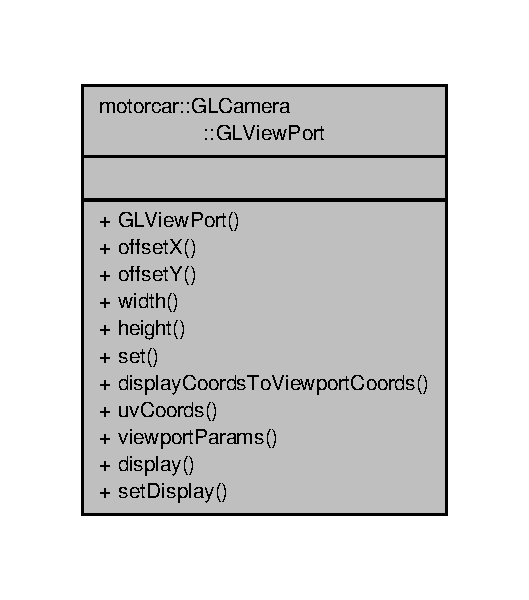
\includegraphics[width=254pt]{classmotorcar_1_1GLCamera_1_1GLViewPort__coll__graph}
\end{center}
\end{figure}
\subsection*{Public Member Functions}
\begin{DoxyCompactItemize}
\item 
\hyperlink{classmotorcar_1_1GLCamera_1_1GLViewPort_a2a9a7ad54eb7e67f5af14961f5e4d473}{G\-L\-View\-Port} (float \hyperlink{classmotorcar_1_1GLCamera_1_1GLViewPort_aec8c3cbf2330c52f6385fd35069057b5}{offset\-X}, float \hyperlink{classmotorcar_1_1GLCamera_1_1GLViewPort_a78b27abaa97aa9723ef16f03bf88422e}{offset\-Y}, float \hyperlink{classmotorcar_1_1GLCamera_1_1GLViewPort_aec2452a157f3d629989ee1ced1c8e16f}{width}, float \hyperlink{classmotorcar_1_1GLCamera_1_1GLViewPort_a8e2b20f86f8c60e2b1088802b84ecd40}{height}, \hyperlink{classmotorcar_1_1Display}{Display} $\ast$\hyperlink{classmotorcar_1_1GLCamera_1_1GLViewPort_a343c2e115a4bbce95ada0fddaff5e75c}{display})
\item 
float \hyperlink{classmotorcar_1_1GLCamera_1_1GLViewPort_aec8c3cbf2330c52f6385fd35069057b5}{offset\-X} () const 
\item 
float \hyperlink{classmotorcar_1_1GLCamera_1_1GLViewPort_a78b27abaa97aa9723ef16f03bf88422e}{offset\-Y} () const 
\item 
float \hyperlink{classmotorcar_1_1GLCamera_1_1GLViewPort_aec2452a157f3d629989ee1ced1c8e16f}{width} () const 
\item 
float \hyperlink{classmotorcar_1_1GLCamera_1_1GLViewPort_a8e2b20f86f8c60e2b1088802b84ecd40}{height} () const 
\item 
void \hyperlink{classmotorcar_1_1GLCamera_1_1GLViewPort_aec5823d6424494e28c6401b5f1032a7a}{set} () const 
\item 
glm\-::vec2 \hyperlink{classmotorcar_1_1GLCamera_1_1GLViewPort_a4195ec0a3331334610640ad1b263e6d0}{display\-Coords\-To\-Viewport\-Coords} (float pixel\-X, float pixel\-Y) const 
\item 
void \hyperlink{classmotorcar_1_1GLCamera_1_1GLViewPort_a615221d4cf7d6edb3c5058e71fff7c42}{uv\-Coords} (float $\ast$buf)
\item 
glm\-::vec4 \hyperlink{classmotorcar_1_1GLCamera_1_1GLViewPort_a5e4c93af53e746fe1dfd187692c0e3c7}{viewport\-Params} () const 
\item 
\hyperlink{classmotorcar_1_1Display}{Display} $\ast$ \hyperlink{classmotorcar_1_1GLCamera_1_1GLViewPort_a343c2e115a4bbce95ada0fddaff5e75c}{display} () const 
\item 
void \hyperlink{classmotorcar_1_1GLCamera_1_1GLViewPort_af061ba79f2457c42a8cd66587c98faf5}{set\-Display} (\hyperlink{classmotorcar_1_1Display}{Display} $\ast$\hyperlink{classmotorcar_1_1GLCamera_1_1GLViewPort_a343c2e115a4bbce95ada0fddaff5e75c}{display})
\end{DoxyCompactItemize}


\subsection{Constructor \& Destructor Documentation}
\hypertarget{classmotorcar_1_1GLCamera_1_1GLViewPort_a2a9a7ad54eb7e67f5af14961f5e4d473}{\index{motorcar\-::\-G\-L\-Camera\-::\-G\-L\-View\-Port@{motorcar\-::\-G\-L\-Camera\-::\-G\-L\-View\-Port}!G\-L\-View\-Port@{G\-L\-View\-Port}}
\index{G\-L\-View\-Port@{G\-L\-View\-Port}!motorcar::GLCamera::GLViewPort@{motorcar\-::\-G\-L\-Camera\-::\-G\-L\-View\-Port}}
\subsubsection[{G\-L\-View\-Port}]{\setlength{\rightskip}{0pt plus 5cm}G\-L\-Camera\-::\-G\-L\-View\-Port\-::\-G\-L\-View\-Port (
\begin{DoxyParamCaption}
\item[{float}]{offset\-X, }
\item[{float}]{offset\-Y, }
\item[{float}]{width, }
\item[{float}]{height, }
\item[{{\bf Display} $\ast$}]{display}
\end{DoxyParamCaption}
)}}\label{classmotorcar_1_1GLCamera_1_1GLViewPort_a2a9a7ad54eb7e67f5af14961f5e4d473}


\subsection{Member Function Documentation}
\hypertarget{classmotorcar_1_1GLCamera_1_1GLViewPort_a343c2e115a4bbce95ada0fddaff5e75c}{\index{motorcar\-::\-G\-L\-Camera\-::\-G\-L\-View\-Port@{motorcar\-::\-G\-L\-Camera\-::\-G\-L\-View\-Port}!display@{display}}
\index{display@{display}!motorcar::GLCamera::GLViewPort@{motorcar\-::\-G\-L\-Camera\-::\-G\-L\-View\-Port}}
\subsubsection[{display}]{\setlength{\rightskip}{0pt plus 5cm}{\bf Display} $\ast$ G\-L\-Camera\-::\-G\-L\-View\-Port\-::display (
\begin{DoxyParamCaption}
{}
\end{DoxyParamCaption}
) const}}\label{classmotorcar_1_1GLCamera_1_1GLViewPort_a343c2e115a4bbce95ada0fddaff5e75c}
\hypertarget{classmotorcar_1_1GLCamera_1_1GLViewPort_a4195ec0a3331334610640ad1b263e6d0}{\index{motorcar\-::\-G\-L\-Camera\-::\-G\-L\-View\-Port@{motorcar\-::\-G\-L\-Camera\-::\-G\-L\-View\-Port}!display\-Coords\-To\-Viewport\-Coords@{display\-Coords\-To\-Viewport\-Coords}}
\index{display\-Coords\-To\-Viewport\-Coords@{display\-Coords\-To\-Viewport\-Coords}!motorcar::GLCamera::GLViewPort@{motorcar\-::\-G\-L\-Camera\-::\-G\-L\-View\-Port}}
\subsubsection[{display\-Coords\-To\-Viewport\-Coords}]{\setlength{\rightskip}{0pt plus 5cm}glm\-::vec2 G\-L\-Camera\-::\-G\-L\-View\-Port\-::display\-Coords\-To\-Viewport\-Coords (
\begin{DoxyParamCaption}
\item[{float}]{pixel\-X, }
\item[{float}]{pixel\-Y}
\end{DoxyParamCaption}
) const}}\label{classmotorcar_1_1GLCamera_1_1GLViewPort_a4195ec0a3331334610640ad1b263e6d0}
\hypertarget{classmotorcar_1_1GLCamera_1_1GLViewPort_a8e2b20f86f8c60e2b1088802b84ecd40}{\index{motorcar\-::\-G\-L\-Camera\-::\-G\-L\-View\-Port@{motorcar\-::\-G\-L\-Camera\-::\-G\-L\-View\-Port}!height@{height}}
\index{height@{height}!motorcar::GLCamera::GLViewPort@{motorcar\-::\-G\-L\-Camera\-::\-G\-L\-View\-Port}}
\subsubsection[{height}]{\setlength{\rightskip}{0pt plus 5cm}float G\-L\-Camera\-::\-G\-L\-View\-Port\-::height (
\begin{DoxyParamCaption}
{}
\end{DoxyParamCaption}
) const}}\label{classmotorcar_1_1GLCamera_1_1GLViewPort_a8e2b20f86f8c60e2b1088802b84ecd40}
\hypertarget{classmotorcar_1_1GLCamera_1_1GLViewPort_aec8c3cbf2330c52f6385fd35069057b5}{\index{motorcar\-::\-G\-L\-Camera\-::\-G\-L\-View\-Port@{motorcar\-::\-G\-L\-Camera\-::\-G\-L\-View\-Port}!offset\-X@{offset\-X}}
\index{offset\-X@{offset\-X}!motorcar::GLCamera::GLViewPort@{motorcar\-::\-G\-L\-Camera\-::\-G\-L\-View\-Port}}
\subsubsection[{offset\-X}]{\setlength{\rightskip}{0pt plus 5cm}float G\-L\-Camera\-::\-G\-L\-View\-Port\-::offset\-X (
\begin{DoxyParamCaption}
{}
\end{DoxyParamCaption}
) const}}\label{classmotorcar_1_1GLCamera_1_1GLViewPort_aec8c3cbf2330c52f6385fd35069057b5}
\hypertarget{classmotorcar_1_1GLCamera_1_1GLViewPort_a78b27abaa97aa9723ef16f03bf88422e}{\index{motorcar\-::\-G\-L\-Camera\-::\-G\-L\-View\-Port@{motorcar\-::\-G\-L\-Camera\-::\-G\-L\-View\-Port}!offset\-Y@{offset\-Y}}
\index{offset\-Y@{offset\-Y}!motorcar::GLCamera::GLViewPort@{motorcar\-::\-G\-L\-Camera\-::\-G\-L\-View\-Port}}
\subsubsection[{offset\-Y}]{\setlength{\rightskip}{0pt plus 5cm}float G\-L\-Camera\-::\-G\-L\-View\-Port\-::offset\-Y (
\begin{DoxyParamCaption}
{}
\end{DoxyParamCaption}
) const}}\label{classmotorcar_1_1GLCamera_1_1GLViewPort_a78b27abaa97aa9723ef16f03bf88422e}
\hypertarget{classmotorcar_1_1GLCamera_1_1GLViewPort_aec5823d6424494e28c6401b5f1032a7a}{\index{motorcar\-::\-G\-L\-Camera\-::\-G\-L\-View\-Port@{motorcar\-::\-G\-L\-Camera\-::\-G\-L\-View\-Port}!set@{set}}
\index{set@{set}!motorcar::GLCamera::GLViewPort@{motorcar\-::\-G\-L\-Camera\-::\-G\-L\-View\-Port}}
\subsubsection[{set}]{\setlength{\rightskip}{0pt plus 5cm}void G\-L\-Camera\-::\-G\-L\-View\-Port\-::set (
\begin{DoxyParamCaption}
{}
\end{DoxyParamCaption}
) const}}\label{classmotorcar_1_1GLCamera_1_1GLViewPort_aec5823d6424494e28c6401b5f1032a7a}
\hypertarget{classmotorcar_1_1GLCamera_1_1GLViewPort_af061ba79f2457c42a8cd66587c98faf5}{\index{motorcar\-::\-G\-L\-Camera\-::\-G\-L\-View\-Port@{motorcar\-::\-G\-L\-Camera\-::\-G\-L\-View\-Port}!set\-Display@{set\-Display}}
\index{set\-Display@{set\-Display}!motorcar::GLCamera::GLViewPort@{motorcar\-::\-G\-L\-Camera\-::\-G\-L\-View\-Port}}
\subsubsection[{set\-Display}]{\setlength{\rightskip}{0pt plus 5cm}void G\-L\-Camera\-::\-G\-L\-View\-Port\-::set\-Display (
\begin{DoxyParamCaption}
\item[{{\bf Display} $\ast$}]{display}
\end{DoxyParamCaption}
)}}\label{classmotorcar_1_1GLCamera_1_1GLViewPort_af061ba79f2457c42a8cd66587c98faf5}
\hypertarget{classmotorcar_1_1GLCamera_1_1GLViewPort_a615221d4cf7d6edb3c5058e71fff7c42}{\index{motorcar\-::\-G\-L\-Camera\-::\-G\-L\-View\-Port@{motorcar\-::\-G\-L\-Camera\-::\-G\-L\-View\-Port}!uv\-Coords@{uv\-Coords}}
\index{uv\-Coords@{uv\-Coords}!motorcar::GLCamera::GLViewPort@{motorcar\-::\-G\-L\-Camera\-::\-G\-L\-View\-Port}}
\subsubsection[{uv\-Coords}]{\setlength{\rightskip}{0pt plus 5cm}void G\-L\-Camera\-::\-G\-L\-View\-Port\-::uv\-Coords (
\begin{DoxyParamCaption}
\item[{float $\ast$}]{buf}
\end{DoxyParamCaption}
)}}\label{classmotorcar_1_1GLCamera_1_1GLViewPort_a615221d4cf7d6edb3c5058e71fff7c42}
\hypertarget{classmotorcar_1_1GLCamera_1_1GLViewPort_a5e4c93af53e746fe1dfd187692c0e3c7}{\index{motorcar\-::\-G\-L\-Camera\-::\-G\-L\-View\-Port@{motorcar\-::\-G\-L\-Camera\-::\-G\-L\-View\-Port}!viewport\-Params@{viewport\-Params}}
\index{viewport\-Params@{viewport\-Params}!motorcar::GLCamera::GLViewPort@{motorcar\-::\-G\-L\-Camera\-::\-G\-L\-View\-Port}}
\subsubsection[{viewport\-Params}]{\setlength{\rightskip}{0pt plus 5cm}glm\-::vec4 G\-L\-Camera\-::\-G\-L\-View\-Port\-::viewport\-Params (
\begin{DoxyParamCaption}
{}
\end{DoxyParamCaption}
) const}}\label{classmotorcar_1_1GLCamera_1_1GLViewPort_a5e4c93af53e746fe1dfd187692c0e3c7}
\hypertarget{classmotorcar_1_1GLCamera_1_1GLViewPort_aec2452a157f3d629989ee1ced1c8e16f}{\index{motorcar\-::\-G\-L\-Camera\-::\-G\-L\-View\-Port@{motorcar\-::\-G\-L\-Camera\-::\-G\-L\-View\-Port}!width@{width}}
\index{width@{width}!motorcar::GLCamera::GLViewPort@{motorcar\-::\-G\-L\-Camera\-::\-G\-L\-View\-Port}}
\subsubsection[{width}]{\setlength{\rightskip}{0pt plus 5cm}float G\-L\-Camera\-::\-G\-L\-View\-Port\-::width (
\begin{DoxyParamCaption}
{}
\end{DoxyParamCaption}
) const}}\label{classmotorcar_1_1GLCamera_1_1GLViewPort_aec2452a157f3d629989ee1ced1c8e16f}


The documentation for this class was generated from the following files\-:\begin{DoxyCompactItemize}
\item 
/home/dave/thesis/qtwayland-\/motorcar-\/compositor/motorcar/src/scenegraph/output/\hyperlink{glcameranode_8h}{glcameranode.\-h}\item 
/home/dave/thesis/qtwayland-\/motorcar-\/compositor/motorcar/src/scenegraph/output/\hyperlink{glcameranode_8cpp}{glcameranode.\-cpp}\end{DoxyCompactItemize}

\hypertarget{classmotorcar_1_1InputElement}{\section{motorcar\-:\-:Input\-Element Class Reference}
\label{classmotorcar_1_1InputElement}\index{motorcar\-::\-Input\-Element@{motorcar\-::\-Input\-Element}}
}


{\ttfamily \#include $<$inputelement.\-h$>$}



Inheritance diagram for motorcar\-:\-:Input\-Element\-:
\nopagebreak
\begin{figure}[H]
\begin{center}
\leavevmode
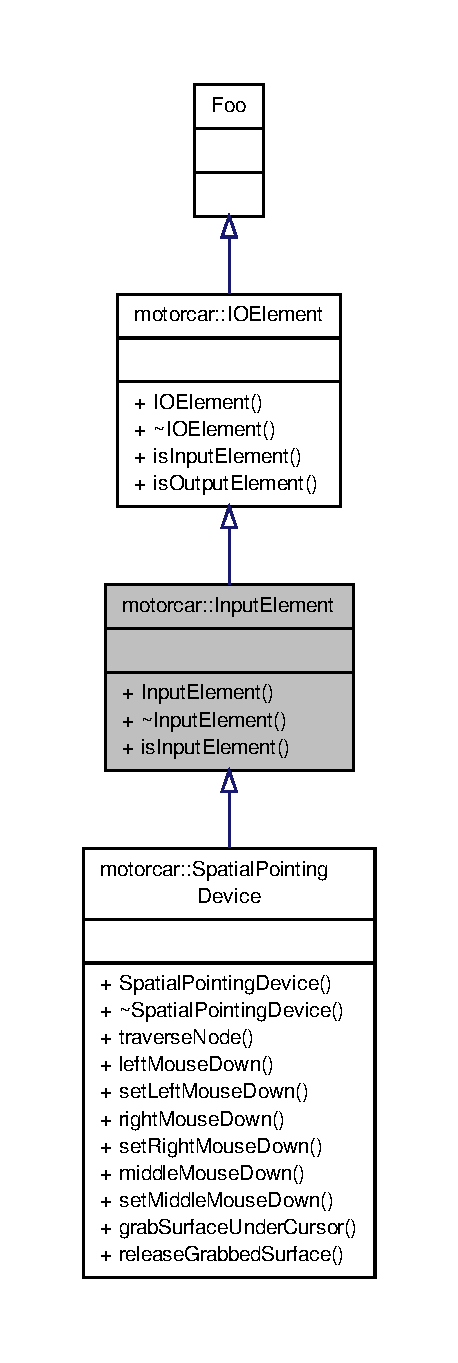
\includegraphics[height=550pt]{classmotorcar_1_1InputElement__inherit__graph}
\end{center}
\end{figure}


Collaboration diagram for motorcar\-:\-:Input\-Element\-:
\nopagebreak
\begin{figure}[H]
\begin{center}
\leavevmode
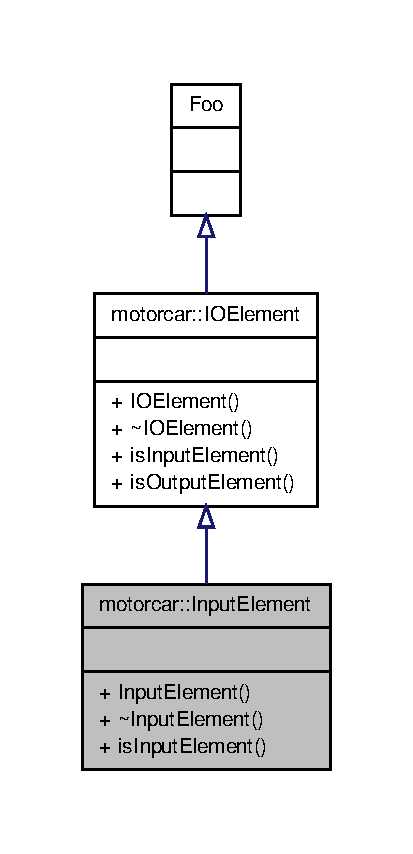
\includegraphics[width=198pt]{classmotorcar_1_1InputElement__coll__graph}
\end{center}
\end{figure}
\subsection*{Public Member Functions}
\begin{DoxyCompactItemize}
\item 
\hyperlink{classmotorcar_1_1InputElement_a7e1f2b5fbda511d4ae48a07764a1ce96}{Input\-Element} ()
\item 
virtual \hyperlink{classmotorcar_1_1InputElement_a79f49cb7f04f2e3bb51cc64cf7eeebfe}{$\sim$\-Input\-Element} ()
\item 
bool \hyperlink{classmotorcar_1_1InputElement_a0ed65040f43f2f699708e424d8d1de48}{is\-Input\-Element} () const 
\end{DoxyCompactItemize}


\subsection{Constructor \& Destructor Documentation}
\hypertarget{classmotorcar_1_1InputElement_a7e1f2b5fbda511d4ae48a07764a1ce96}{\index{motorcar\-::\-Input\-Element@{motorcar\-::\-Input\-Element}!Input\-Element@{Input\-Element}}
\index{Input\-Element@{Input\-Element}!motorcar::InputElement@{motorcar\-::\-Input\-Element}}
\subsubsection[{Input\-Element}]{\setlength{\rightskip}{0pt plus 5cm}Input\-Element\-::\-Input\-Element (
\begin{DoxyParamCaption}
{}
\end{DoxyParamCaption}
)}}\label{classmotorcar_1_1InputElement_a7e1f2b5fbda511d4ae48a07764a1ce96}
\hypertarget{classmotorcar_1_1InputElement_a79f49cb7f04f2e3bb51cc64cf7eeebfe}{\index{motorcar\-::\-Input\-Element@{motorcar\-::\-Input\-Element}!$\sim$\-Input\-Element@{$\sim$\-Input\-Element}}
\index{$\sim$\-Input\-Element@{$\sim$\-Input\-Element}!motorcar::InputElement@{motorcar\-::\-Input\-Element}}
\subsubsection[{$\sim$\-Input\-Element}]{\setlength{\rightskip}{0pt plus 5cm}virtual motorcar\-::\-Input\-Element\-::$\sim$\-Input\-Element (
\begin{DoxyParamCaption}
{}
\end{DoxyParamCaption}
)\hspace{0.3cm}{\ttfamily [inline]}, {\ttfamily [virtual]}}}\label{classmotorcar_1_1InputElement_a79f49cb7f04f2e3bb51cc64cf7eeebfe}


\subsection{Member Function Documentation}
\hypertarget{classmotorcar_1_1InputElement_a0ed65040f43f2f699708e424d8d1de48}{\index{motorcar\-::\-Input\-Element@{motorcar\-::\-Input\-Element}!is\-Input\-Element@{is\-Input\-Element}}
\index{is\-Input\-Element@{is\-Input\-Element}!motorcar::InputElement@{motorcar\-::\-Input\-Element}}
\subsubsection[{is\-Input\-Element}]{\setlength{\rightskip}{0pt plus 5cm}bool Input\-Element\-::is\-Input\-Element (
\begin{DoxyParamCaption}
{}
\end{DoxyParamCaption}
) const\hspace{0.3cm}{\ttfamily [virtual]}}}\label{classmotorcar_1_1InputElement_a0ed65040f43f2f699708e424d8d1de48}


Implements \hyperlink{classmotorcar_1_1IOElement_ab73b2687c5452ff694f20c40357ee219}{motorcar\-::\-I\-O\-Element}.



The documentation for this class was generated from the following files\-:\begin{DoxyCompactItemize}
\item 
/home/dave/thesis/qtwayland-\/motorcar-\/compositor/motorcar/src/scenegraph/input/\hyperlink{inputelement_8h}{inputelement.\-h}\item 
/home/dave/thesis/qtwayland-\/motorcar-\/compositor/motorcar/src/scenegraph/input/\hyperlink{inputelement_8cpp}{inputelement.\-cpp}\end{DoxyCompactItemize}

\hypertarget{classmotorcar_1_1IOElement}{\section{motorcar\-:\-:I\-O\-Element Class Reference}
\label{classmotorcar_1_1IOElement}\index{motorcar\-::\-I\-O\-Element@{motorcar\-::\-I\-O\-Element}}
}


{\ttfamily \#include $<$ioelement.\-h$>$}



Inheritance diagram for motorcar\-:\-:I\-O\-Element\-:
\nopagebreak
\begin{figure}[H]
\begin{center}
\leavevmode
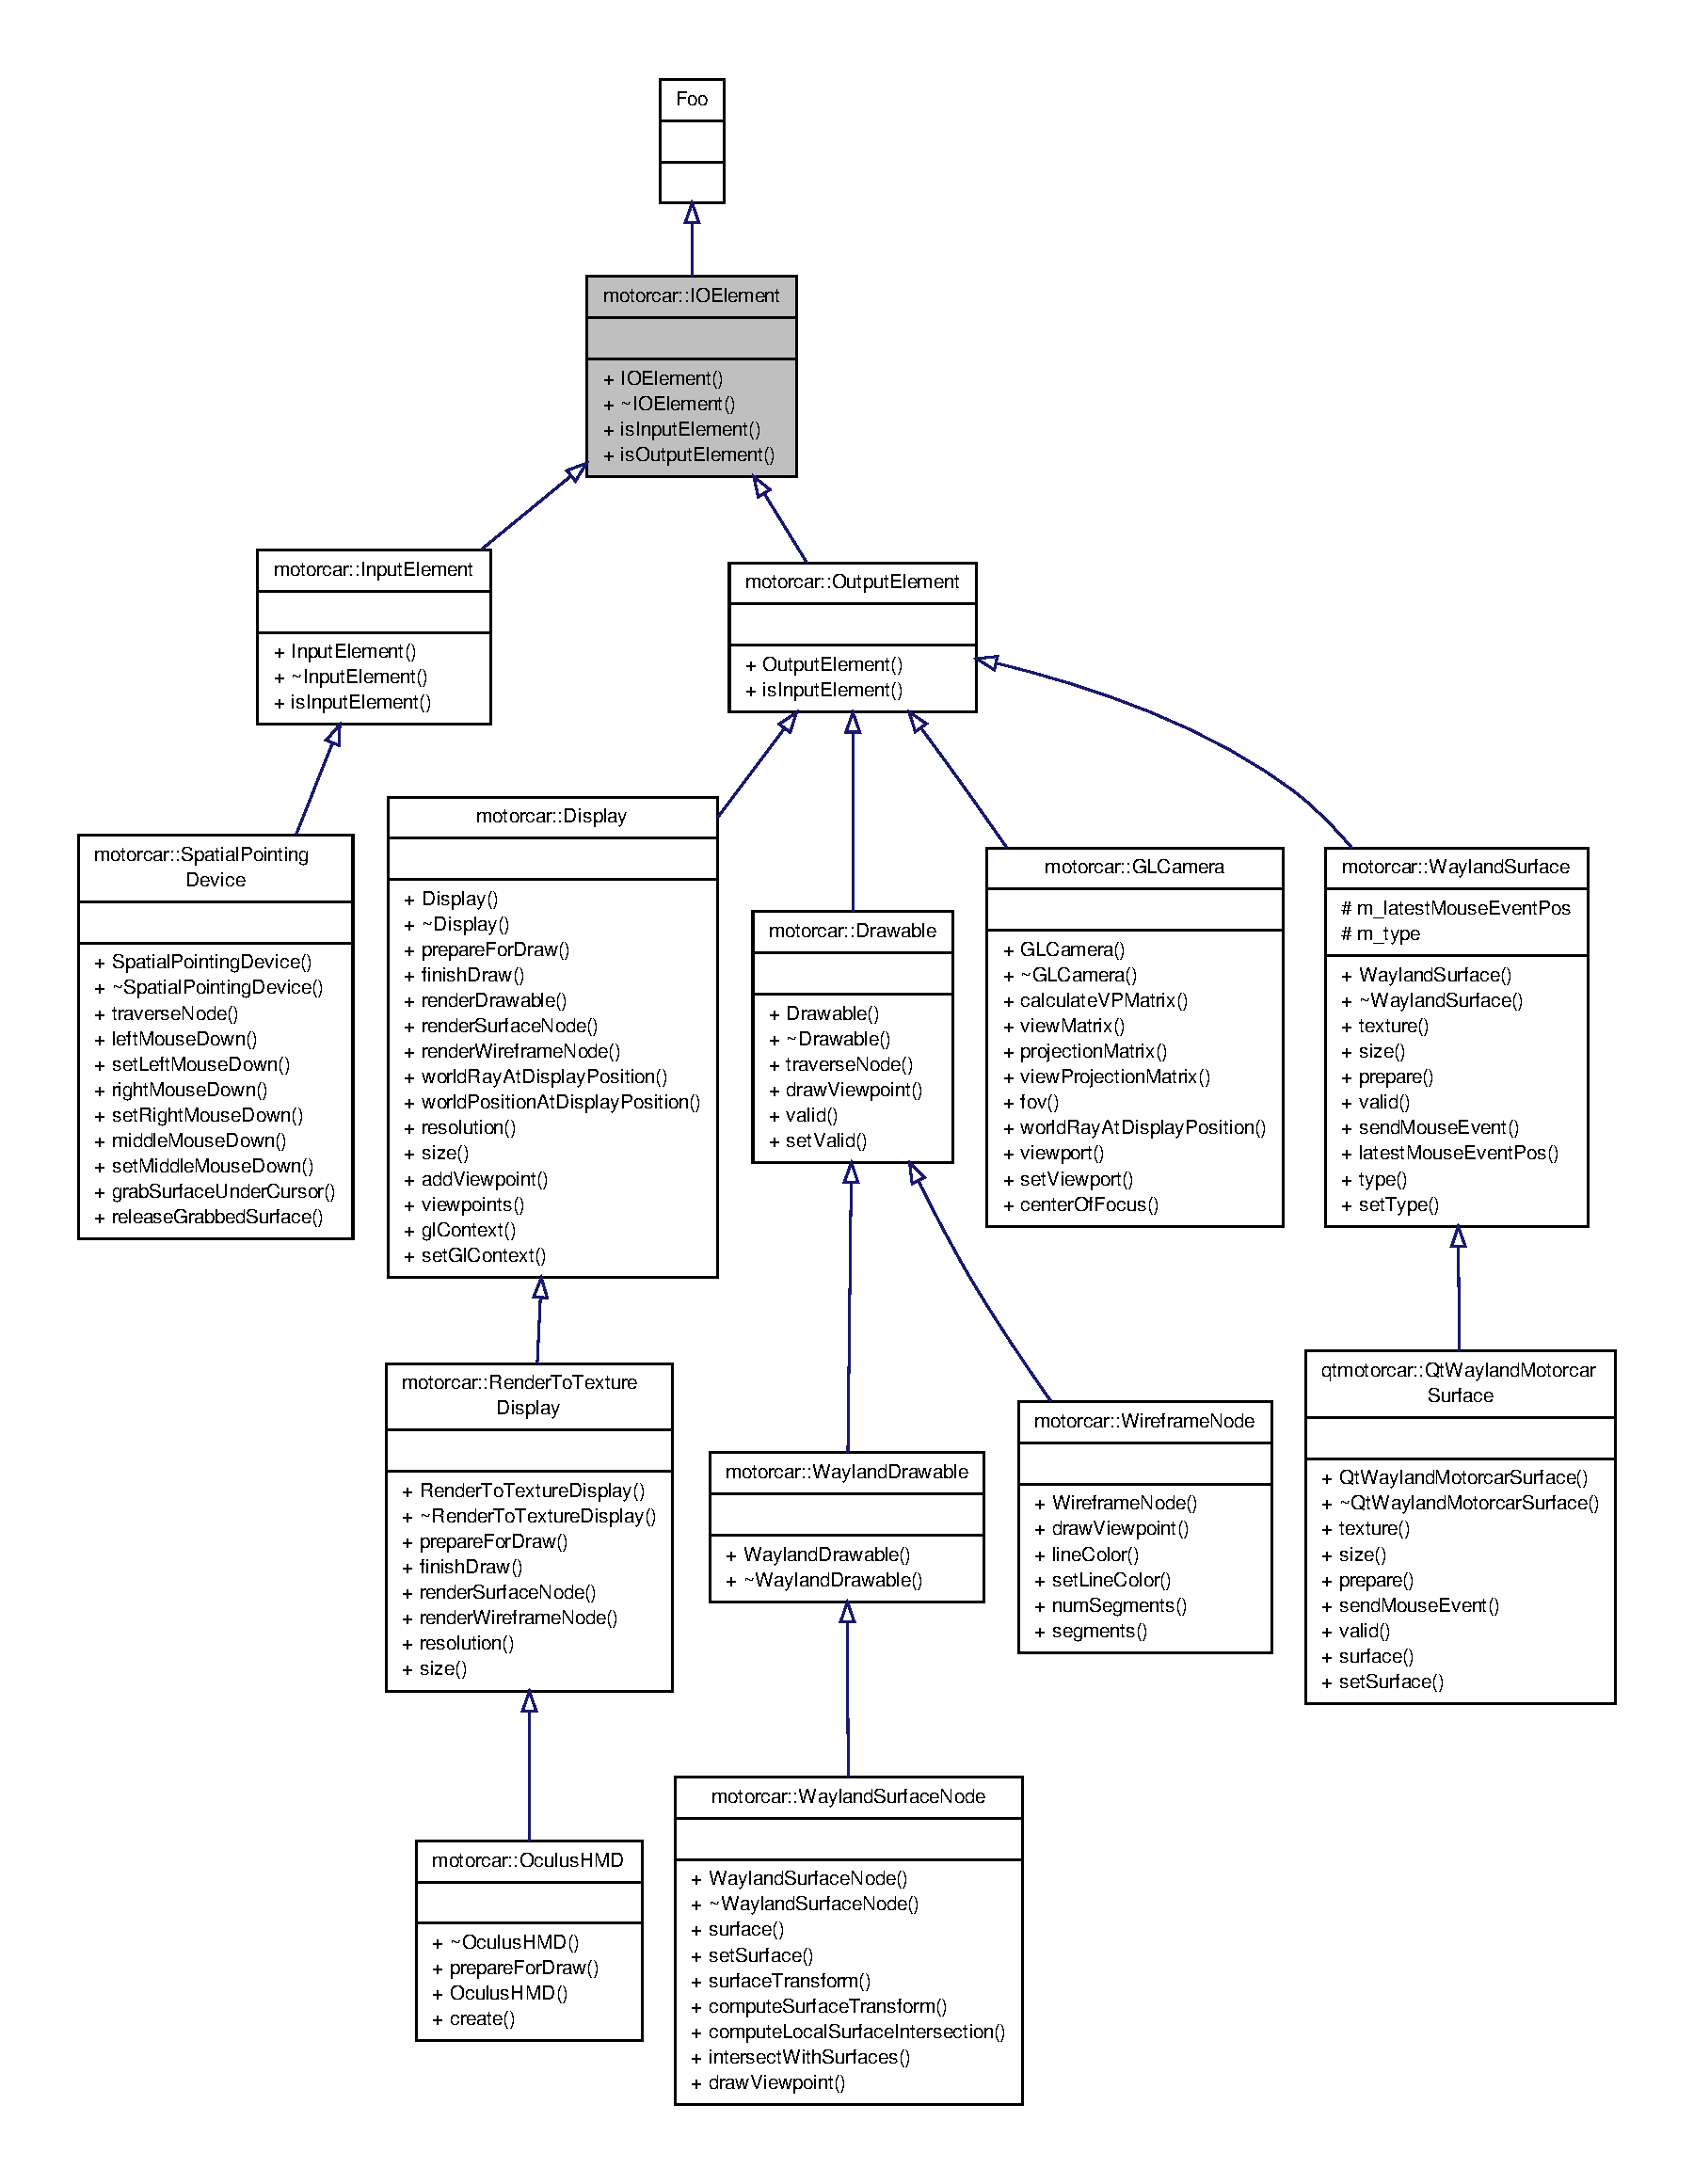
\includegraphics[width=350pt]{classmotorcar_1_1IOElement__inherit__graph}
\end{center}
\end{figure}


Collaboration diagram for motorcar\-:\-:I\-O\-Element\-:
\nopagebreak
\begin{figure}[H]
\begin{center}
\leavevmode
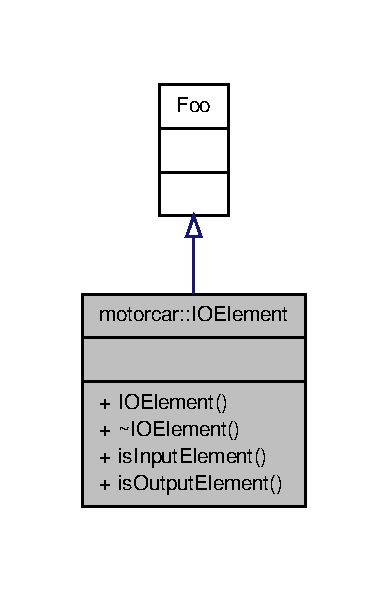
\includegraphics[width=186pt]{classmotorcar_1_1IOElement__coll__graph}
\end{center}
\end{figure}
\subsection*{Public Member Functions}
\begin{DoxyCompactItemize}
\item 
\hyperlink{classmotorcar_1_1IOElement_aca2725fb65626d1cc50a12192cf5b52b}{I\-O\-Element} ()
\item 
virtual \hyperlink{classmotorcar_1_1IOElement_a6b771ea66fd530dbec633514a490978d}{$\sim$\-I\-O\-Element} ()
\item 
virtual bool \hyperlink{classmotorcar_1_1IOElement_ab73b2687c5452ff694f20c40357ee219}{is\-Input\-Element} () const =0
\item 
bool \hyperlink{classmotorcar_1_1IOElement_a0f451058d4d845c9ffd93c7c0f11af1b}{is\-Output\-Element} () const 
\end{DoxyCompactItemize}


\subsection{Constructor \& Destructor Documentation}
\hypertarget{classmotorcar_1_1IOElement_aca2725fb65626d1cc50a12192cf5b52b}{\index{motorcar\-::\-I\-O\-Element@{motorcar\-::\-I\-O\-Element}!I\-O\-Element@{I\-O\-Element}}
\index{I\-O\-Element@{I\-O\-Element}!motorcar::IOElement@{motorcar\-::\-I\-O\-Element}}
\subsubsection[{I\-O\-Element}]{\setlength{\rightskip}{0pt plus 5cm}I\-O\-Element\-::\-I\-O\-Element (
\begin{DoxyParamCaption}
{}
\end{DoxyParamCaption}
)}}\label{classmotorcar_1_1IOElement_aca2725fb65626d1cc50a12192cf5b52b}
\hypertarget{classmotorcar_1_1IOElement_a6b771ea66fd530dbec633514a490978d}{\index{motorcar\-::\-I\-O\-Element@{motorcar\-::\-I\-O\-Element}!$\sim$\-I\-O\-Element@{$\sim$\-I\-O\-Element}}
\index{$\sim$\-I\-O\-Element@{$\sim$\-I\-O\-Element}!motorcar::IOElement@{motorcar\-::\-I\-O\-Element}}
\subsubsection[{$\sim$\-I\-O\-Element}]{\setlength{\rightskip}{0pt plus 5cm}virtual motorcar\-::\-I\-O\-Element\-::$\sim$\-I\-O\-Element (
\begin{DoxyParamCaption}
{}
\end{DoxyParamCaption}
)\hspace{0.3cm}{\ttfamily [inline]}, {\ttfamily [virtual]}}}\label{classmotorcar_1_1IOElement_a6b771ea66fd530dbec633514a490978d}


\subsection{Member Function Documentation}
\hypertarget{classmotorcar_1_1IOElement_ab73b2687c5452ff694f20c40357ee219}{\index{motorcar\-::\-I\-O\-Element@{motorcar\-::\-I\-O\-Element}!is\-Input\-Element@{is\-Input\-Element}}
\index{is\-Input\-Element@{is\-Input\-Element}!motorcar::IOElement@{motorcar\-::\-I\-O\-Element}}
\subsubsection[{is\-Input\-Element}]{\setlength{\rightskip}{0pt plus 5cm}virtual bool motorcar\-::\-I\-O\-Element\-::is\-Input\-Element (
\begin{DoxyParamCaption}
{}
\end{DoxyParamCaption}
) const\hspace{0.3cm}{\ttfamily [pure virtual]}}}\label{classmotorcar_1_1IOElement_ab73b2687c5452ff694f20c40357ee219}


Implemented in \hyperlink{classmotorcar_1_1InputElement_a0ed65040f43f2f699708e424d8d1de48}{motorcar\-::\-Input\-Element}, and \hyperlink{classmotorcar_1_1OutputElement_a4edec9c114aabe4adf60fee24e8468de}{motorcar\-::\-Output\-Element}.

\hypertarget{classmotorcar_1_1IOElement_a0f451058d4d845c9ffd93c7c0f11af1b}{\index{motorcar\-::\-I\-O\-Element@{motorcar\-::\-I\-O\-Element}!is\-Output\-Element@{is\-Output\-Element}}
\index{is\-Output\-Element@{is\-Output\-Element}!motorcar::IOElement@{motorcar\-::\-I\-O\-Element}}
\subsubsection[{is\-Output\-Element}]{\setlength{\rightskip}{0pt plus 5cm}bool I\-O\-Element\-::is\-Output\-Element (
\begin{DoxyParamCaption}
{}
\end{DoxyParamCaption}
) const}}\label{classmotorcar_1_1IOElement_a0f451058d4d845c9ffd93c7c0f11af1b}


The documentation for this class was generated from the following files\-:\begin{DoxyCompactItemize}
\item 
/home/dave/thesis/qtwayland-\/motorcar-\/compositor/motorcar/src/scenegraph/\hyperlink{ioelement_8h}{ioelement.\-h}\item 
/home/dave/thesis/qtwayland-\/motorcar-\/compositor/motorcar/src/scenegraph/\hyperlink{ioelement_8cpp}{ioelement.\-cpp}\end{DoxyCompactItemize}

\hypertarget{classmotorcar_1_1OculusHMD}{\section{motorcar\-:\-:Oculus\-H\-M\-D Class Reference}
\label{classmotorcar_1_1OculusHMD}\index{motorcar\-::\-Oculus\-H\-M\-D@{motorcar\-::\-Oculus\-H\-M\-D}}
}


{\ttfamily \#include $<$oculushmd.\-h$>$}



Inheritance diagram for motorcar\-:\-:Oculus\-H\-M\-D\-:
\nopagebreak
\begin{figure}[H]
\begin{center}
\leavevmode
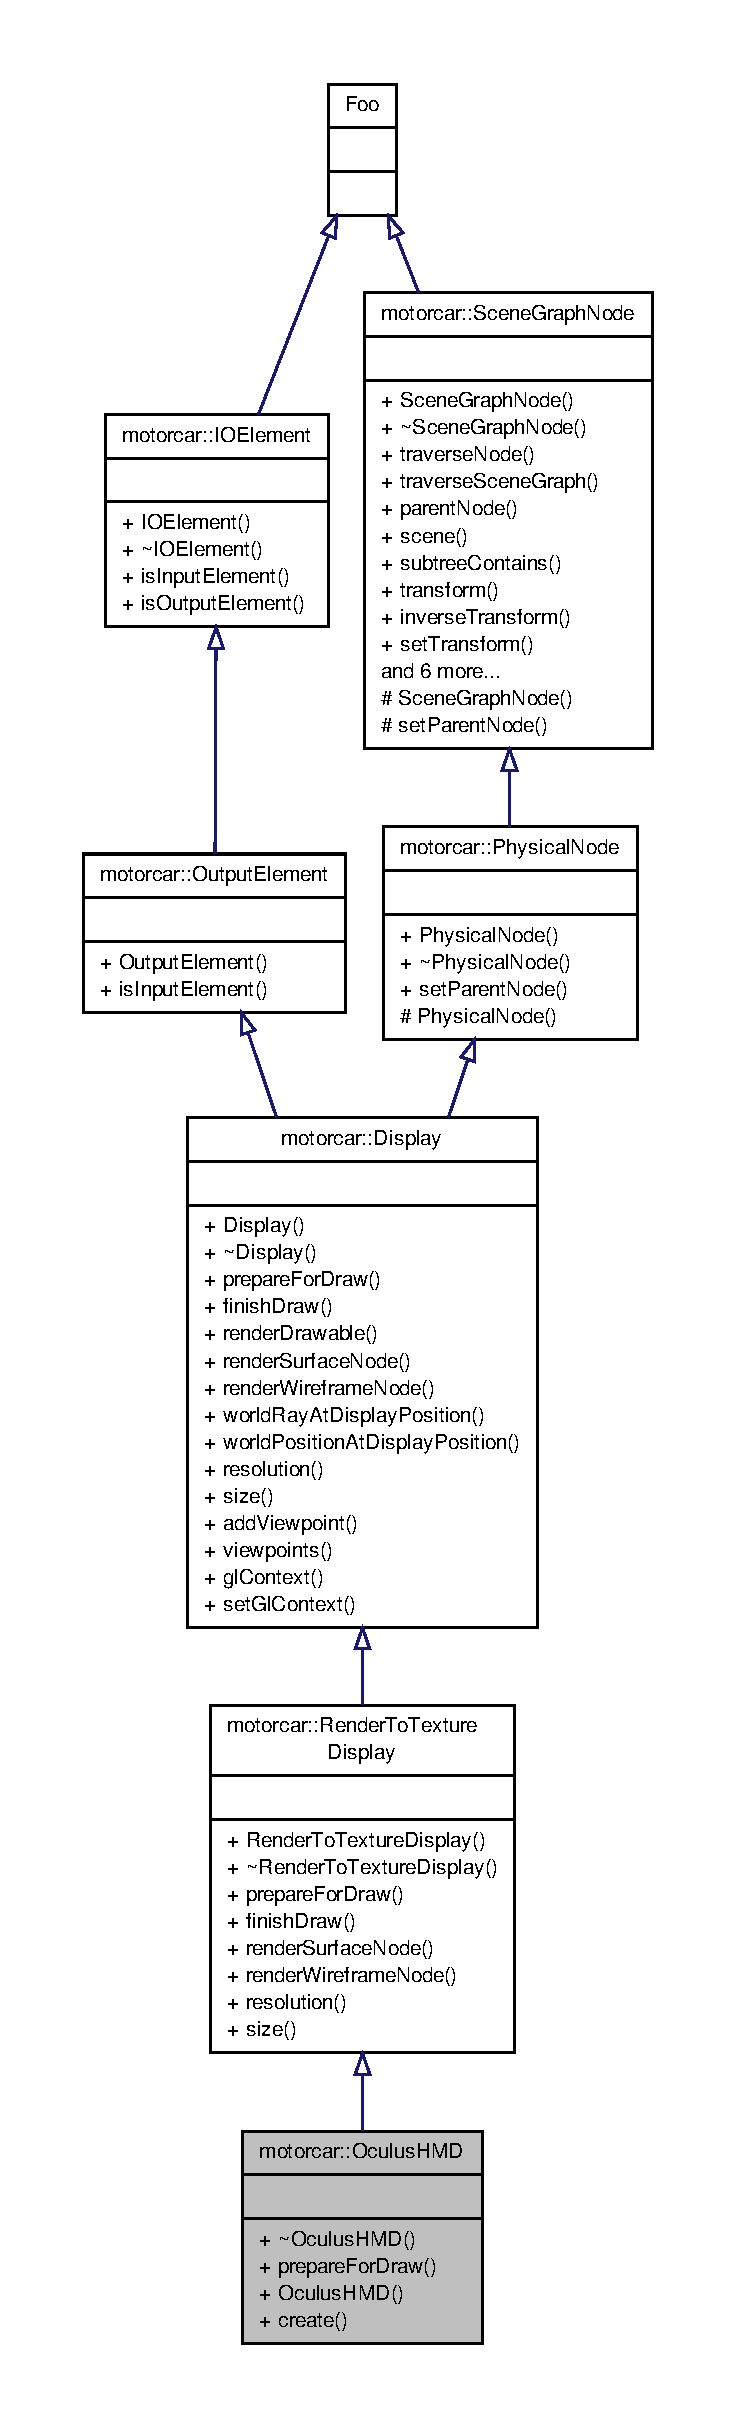
\includegraphics[width=332pt]{classmotorcar_1_1OculusHMD__inherit__graph}
\end{center}
\end{figure}


Collaboration diagram for motorcar\-:\-:Oculus\-H\-M\-D\-:
\nopagebreak
\begin{figure}[H]
\begin{center}
\leavevmode
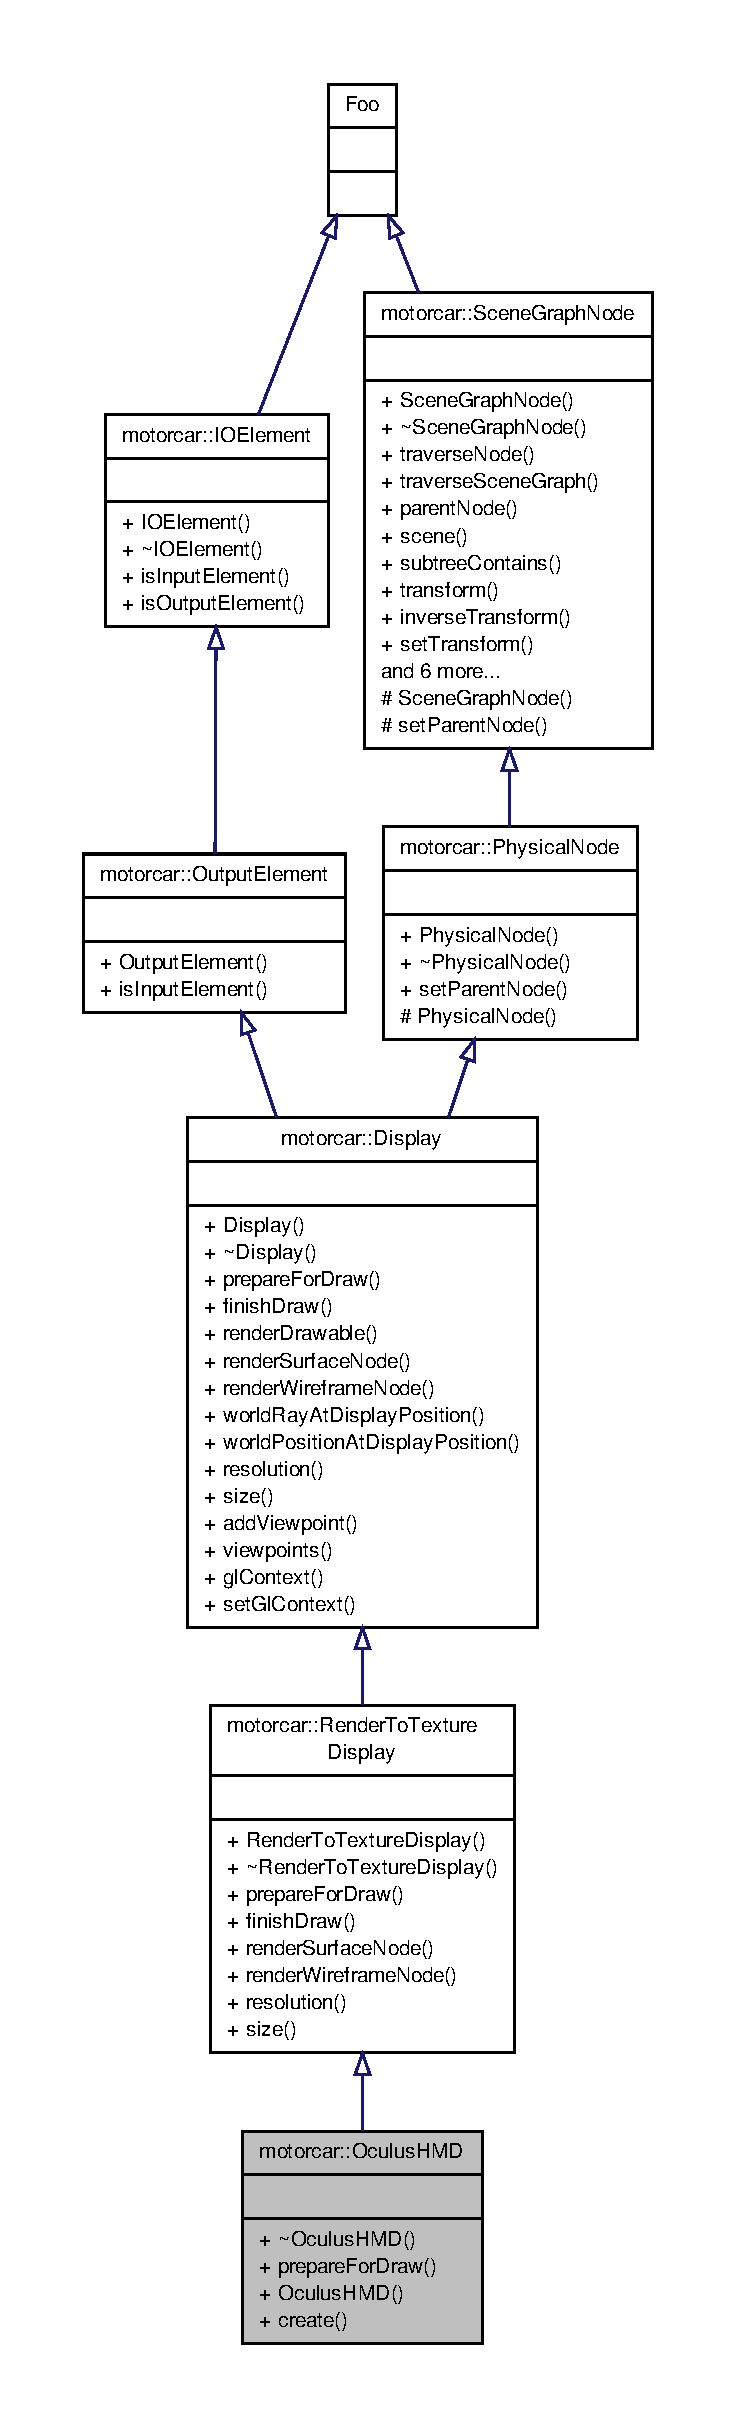
\includegraphics[width=332pt]{classmotorcar_1_1OculusHMD__coll__graph}
\end{center}
\end{figure}
\subsection*{Public Member Functions}
\begin{DoxyCompactItemize}
\item 
\hyperlink{classmotorcar_1_1OculusHMD_a69e38487ae0a51504663dd942fbb068e}{$\sim$\-Oculus\-H\-M\-D} ()
\item 
void \hyperlink{classmotorcar_1_1OculusHMD_ae9834ea50d728809532b7a48f7ed1738}{prepare\-For\-Draw} () override
\item 
\hyperlink{classmotorcar_1_1OculusHMD_a4f64cac13d749bf6d0cc9ca1f94297bb}{Oculus\-H\-M\-D} (O\-V\-R\-System $\ast$system, \hyperlink{classmotorcar_1_1Skeleton}{Skeleton} $\ast$skeleton, float scale, glm\-::vec4 distortion\-K, \hyperlink{classmotorcar_1_1OpenGLContext}{Open\-G\-L\-Context} $\ast$\hyperlink{classmotorcar_1_1Display_a884dd0b78dbecee82a33eb6d26a2a403}{gl\-Context}, glm\-::vec2 display\-Dimensions, \hyperlink{classmotorcar_1_1PhysicalNode}{Physical\-Node} $\ast$parent, const glm\-::mat4 \&\hyperlink{classmotorcar_1_1SceneGraphNode_ad96e79fdd739ac8223a3128003be391a}{transform})
\end{DoxyCompactItemize}
\subsection*{Static Public Member Functions}
\begin{DoxyCompactItemize}
\item 
static \hyperlink{classmotorcar_1_1OculusHMD}{Oculus\-H\-M\-D} $\ast$ \hyperlink{classmotorcar_1_1OculusHMD_aa77e2ef2bda8701075d5e669c95cc3ce}{create} (\hyperlink{classmotorcar_1_1OpenGLContext}{Open\-G\-L\-Context} $\ast$\hyperlink{classmotorcar_1_1Display_a884dd0b78dbecee82a33eb6d26a2a403}{gl\-Context}, \hyperlink{classmotorcar_1_1Skeleton}{Skeleton} $\ast$skeleton, \hyperlink{classmotorcar_1_1PhysicalNode}{Physical\-Node} $\ast$parent)
\end{DoxyCompactItemize}
\subsection*{Additional Inherited Members}


\subsection{Constructor \& Destructor Documentation}
\hypertarget{classmotorcar_1_1OculusHMD_a69e38487ae0a51504663dd942fbb068e}{\index{motorcar\-::\-Oculus\-H\-M\-D@{motorcar\-::\-Oculus\-H\-M\-D}!$\sim$\-Oculus\-H\-M\-D@{$\sim$\-Oculus\-H\-M\-D}}
\index{$\sim$\-Oculus\-H\-M\-D@{$\sim$\-Oculus\-H\-M\-D}!motorcar::OculusHMD@{motorcar\-::\-Oculus\-H\-M\-D}}
\subsubsection[{$\sim$\-Oculus\-H\-M\-D}]{\setlength{\rightskip}{0pt plus 5cm}Oculus\-H\-M\-D\-::$\sim$\-Oculus\-H\-M\-D (
\begin{DoxyParamCaption}
{}
\end{DoxyParamCaption}
)}}\label{classmotorcar_1_1OculusHMD_a69e38487ae0a51504663dd942fbb068e}
\hypertarget{classmotorcar_1_1OculusHMD_a4f64cac13d749bf6d0cc9ca1f94297bb}{\index{motorcar\-::\-Oculus\-H\-M\-D@{motorcar\-::\-Oculus\-H\-M\-D}!Oculus\-H\-M\-D@{Oculus\-H\-M\-D}}
\index{Oculus\-H\-M\-D@{Oculus\-H\-M\-D}!motorcar::OculusHMD@{motorcar\-::\-Oculus\-H\-M\-D}}
\subsubsection[{Oculus\-H\-M\-D}]{\setlength{\rightskip}{0pt plus 5cm}Oculus\-H\-M\-D\-::\-Oculus\-H\-M\-D (
\begin{DoxyParamCaption}
\item[{O\-V\-R\-System $\ast$}]{system, }
\item[{{\bf Skeleton} $\ast$}]{skeleton, }
\item[{float}]{scale, }
\item[{glm\-::vec4}]{distortion\-K, }
\item[{{\bf Open\-G\-L\-Context} $\ast$}]{gl\-Context, }
\item[{glm\-::vec2}]{display\-Dimensions, }
\item[{{\bf Physical\-Node} $\ast$}]{parent, }
\item[{const glm\-::mat4 \&}]{transform}
\end{DoxyParamCaption}
)}}\label{classmotorcar_1_1OculusHMD_a4f64cac13d749bf6d0cc9ca1f94297bb}


\subsection{Member Function Documentation}
\hypertarget{classmotorcar_1_1OculusHMD_aa77e2ef2bda8701075d5e669c95cc3ce}{\index{motorcar\-::\-Oculus\-H\-M\-D@{motorcar\-::\-Oculus\-H\-M\-D}!create@{create}}
\index{create@{create}!motorcar::OculusHMD@{motorcar\-::\-Oculus\-H\-M\-D}}
\subsubsection[{create}]{\setlength{\rightskip}{0pt plus 5cm}{\bf Oculus\-H\-M\-D} $\ast$ Oculus\-H\-M\-D\-::create (
\begin{DoxyParamCaption}
\item[{{\bf Open\-G\-L\-Context} $\ast$}]{gl\-Context, }
\item[{{\bf Skeleton} $\ast$}]{skeleton, }
\item[{{\bf Physical\-Node} $\ast$}]{parent}
\end{DoxyParamCaption}
)\hspace{0.3cm}{\ttfamily [static]}}}\label{classmotorcar_1_1OculusHMD_aa77e2ef2bda8701075d5e669c95cc3ce}
\hypertarget{classmotorcar_1_1OculusHMD_ae9834ea50d728809532b7a48f7ed1738}{\index{motorcar\-::\-Oculus\-H\-M\-D@{motorcar\-::\-Oculus\-H\-M\-D}!prepare\-For\-Draw@{prepare\-For\-Draw}}
\index{prepare\-For\-Draw@{prepare\-For\-Draw}!motorcar::OculusHMD@{motorcar\-::\-Oculus\-H\-M\-D}}
\subsubsection[{prepare\-For\-Draw}]{\setlength{\rightskip}{0pt plus 5cm}void Oculus\-H\-M\-D\-::prepare\-For\-Draw (
\begin{DoxyParamCaption}
{}
\end{DoxyParamCaption}
)\hspace{0.3cm}{\ttfamily [override]}, {\ttfamily [virtual]}}}\label{classmotorcar_1_1OculusHMD_ae9834ea50d728809532b7a48f7ed1738}


Reimplemented from \hyperlink{classmotorcar_1_1RenderToTextureDisplay_abdf6861fe69ada64fafd0a7713391bed}{motorcar\-::\-Render\-To\-Texture\-Display}.



The documentation for this class was generated from the following files\-:\begin{DoxyCompactItemize}
\item 
/media/dave/e89b5eb4-\/4b10-\/4edf-\/8ad5-\/0d046a46b978/dave/thesis/qtwayland-\/motorcar-\/compositor/motorcar/src/device/\hyperlink{oculushmd_8h}{oculushmd.\-h}\item 
/media/dave/e89b5eb4-\/4b10-\/4edf-\/8ad5-\/0d046a46b978/dave/thesis/qtwayland-\/motorcar-\/compositor/motorcar/src/device/\hyperlink{oculushmd_8cpp}{oculushmd.\-cpp}\end{DoxyCompactItemize}

\hypertarget{classmotorcar_1_1OpenGLContext}{\section{motorcar\-:\-:Open\-G\-L\-Context Class Reference}
\label{classmotorcar_1_1OpenGLContext}\index{motorcar\-::\-Open\-G\-L\-Context@{motorcar\-::\-Open\-G\-L\-Context}}
}


{\ttfamily \#include $<$openglcontext.\-h$>$}



Inheritance diagram for motorcar\-:\-:Open\-G\-L\-Context\-:
\nopagebreak
\begin{figure}[H]
\begin{center}
\leavevmode
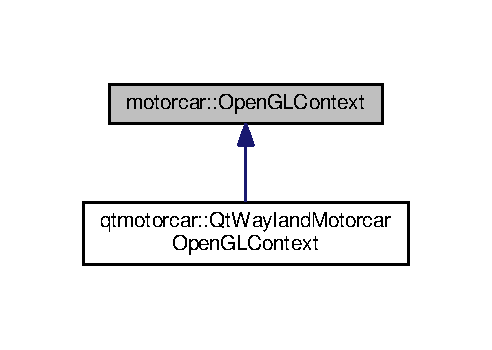
\includegraphics[width=236pt]{classmotorcar_1_1OpenGLContext__inherit__graph}
\end{center}
\end{figure}
\subsection*{Public Member Functions}
\begin{DoxyCompactItemize}
\item 
virtual \hyperlink{classmotorcar_1_1OpenGLContext_ac43c528ca955c030567c0654f171a680}{$\sim$\-Open\-G\-L\-Context} ()
\item 
virtual glm\-::ivec2 \hyperlink{classmotorcar_1_1OpenGLContext_a4a60274f217b9d71ff54ad60351b4127}{default\-Framebuffer\-Size} ()=0
\item 
virtual void \hyperlink{classmotorcar_1_1OpenGLContext_ae8b9c712092d01b69766469ab196ab80}{make\-Current} ()=0
\end{DoxyCompactItemize}


\subsection{Constructor \& Destructor Documentation}
\hypertarget{classmotorcar_1_1OpenGLContext_ac43c528ca955c030567c0654f171a680}{\index{motorcar\-::\-Open\-G\-L\-Context@{motorcar\-::\-Open\-G\-L\-Context}!$\sim$\-Open\-G\-L\-Context@{$\sim$\-Open\-G\-L\-Context}}
\index{$\sim$\-Open\-G\-L\-Context@{$\sim$\-Open\-G\-L\-Context}!motorcar::OpenGLContext@{motorcar\-::\-Open\-G\-L\-Context}}
\subsubsection[{$\sim$\-Open\-G\-L\-Context}]{\setlength{\rightskip}{0pt plus 5cm}virtual motorcar\-::\-Open\-G\-L\-Context\-::$\sim$\-Open\-G\-L\-Context (
\begin{DoxyParamCaption}
{}
\end{DoxyParamCaption}
)\hspace{0.3cm}{\ttfamily [inline]}, {\ttfamily [virtual]}}}\label{classmotorcar_1_1OpenGLContext_ac43c528ca955c030567c0654f171a680}


\subsection{Member Function Documentation}
\hypertarget{classmotorcar_1_1OpenGLContext_a4a60274f217b9d71ff54ad60351b4127}{\index{motorcar\-::\-Open\-G\-L\-Context@{motorcar\-::\-Open\-G\-L\-Context}!default\-Framebuffer\-Size@{default\-Framebuffer\-Size}}
\index{default\-Framebuffer\-Size@{default\-Framebuffer\-Size}!motorcar::OpenGLContext@{motorcar\-::\-Open\-G\-L\-Context}}
\subsubsection[{default\-Framebuffer\-Size}]{\setlength{\rightskip}{0pt plus 5cm}virtual glm\-::ivec2 motorcar\-::\-Open\-G\-L\-Context\-::default\-Framebuffer\-Size (
\begin{DoxyParamCaption}
{}
\end{DoxyParamCaption}
)\hspace{0.3cm}{\ttfamily [pure virtual]}}}\label{classmotorcar_1_1OpenGLContext_a4a60274f217b9d71ff54ad60351b4127}


Implemented in \hyperlink{classqtmotorcar_1_1QtWaylandMotorcarOpenGLContext_ab2a51af3b29de69f0a2d3d60d3bdbe82}{qtmotorcar\-::\-Qt\-Wayland\-Motorcar\-Open\-G\-L\-Context}.

\hypertarget{classmotorcar_1_1OpenGLContext_ae8b9c712092d01b69766469ab196ab80}{\index{motorcar\-::\-Open\-G\-L\-Context@{motorcar\-::\-Open\-G\-L\-Context}!make\-Current@{make\-Current}}
\index{make\-Current@{make\-Current}!motorcar::OpenGLContext@{motorcar\-::\-Open\-G\-L\-Context}}
\subsubsection[{make\-Current}]{\setlength{\rightskip}{0pt plus 5cm}virtual void motorcar\-::\-Open\-G\-L\-Context\-::make\-Current (
\begin{DoxyParamCaption}
{}
\end{DoxyParamCaption}
)\hspace{0.3cm}{\ttfamily [pure virtual]}}}\label{classmotorcar_1_1OpenGLContext_ae8b9c712092d01b69766469ab196ab80}


Implemented in \hyperlink{classqtmotorcar_1_1QtWaylandMotorcarOpenGLContext_ae5f00ad8258f7c03466ad114b64e250a}{qtmotorcar\-::\-Qt\-Wayland\-Motorcar\-Open\-G\-L\-Context}.



The documentation for this class was generated from the following file\-:\begin{DoxyCompactItemize}
\item 
/media/dave/e89b5eb4-\/4b10-\/4edf-\/8ad5-\/0d046a46b978/dave/thesis/qtwayland-\/motorcar-\/compositor/motorcar/src/gl/\hyperlink{openglcontext_8h}{openglcontext.\-h}\end{DoxyCompactItemize}

\hypertarget{classOpenGLData}{\section{Open\-G\-L\-Data Class Reference}
\label{classOpenGLData}\index{Open\-G\-L\-Data@{Open\-G\-L\-Data}}
}


{\ttfamily \#include $<$opengldata.\-h$>$}



Collaboration diagram for Open\-G\-L\-Data\-:
\nopagebreak
\begin{figure}[H]
\begin{center}
\leavevmode
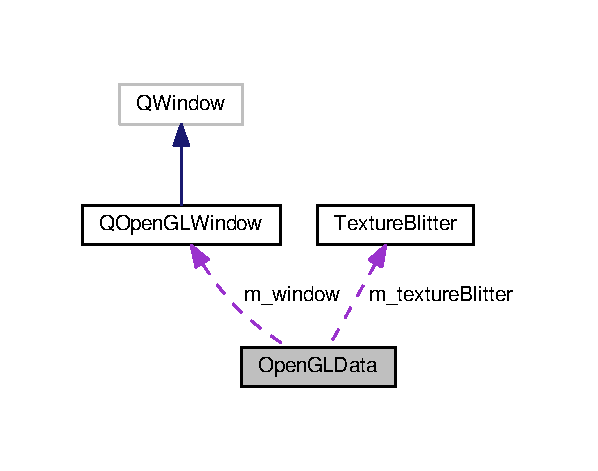
\includegraphics[width=287pt]{classOpenGLData__coll__graph}
\end{center}
\end{figure}
\subsection*{Public Member Functions}
\begin{DoxyCompactItemize}
\item 
\hyperlink{classOpenGLData_ae45b74d0a593e043189b8118e6abcb23}{Open\-G\-L\-Data} (\hyperlink{classQOpenGLWindow}{Q\-Open\-G\-L\-Window} $\ast$\hyperlink{structwindow}{window})
\item 
\hyperlink{classOpenGLData_a9241741339383a555a7189f472006a22}{$\sim$\-Open\-G\-L\-Data} ()
\item 
float \hyperlink{classOpenGLData_a8345c6c7bb79a3e48dfea00b786525c7}{ppcm} ()
\end{DoxyCompactItemize}
\subsection*{Public Attributes}
\begin{DoxyCompactItemize}
\item 
\hyperlink{classQOpenGLWindow}{Q\-Open\-G\-L\-Window} $\ast$ \hyperlink{classOpenGLData_ad4867a83945326a3523a1aa54bc1f016}{m\-\_\-window}
\item 
\hyperlink{classTextureBlitter}{Texture\-Blitter} $\ast$ \hyperlink{classOpenGLData_a7dce95e56b9349ca3a9d048ccc712748}{m\-\_\-texture\-Blitter}
\item 
Q\-Open\-G\-L\-Texture\-Cache $\ast$ \hyperlink{classOpenGLData_ac4c99b1032b6af264e738d02bdba4860}{m\-\_\-texture\-Cache}
\item 
G\-Luint \hyperlink{classOpenGLData_a0480263528e20beed53a1520272b296e}{m\-\_\-surface\-\_\-fbo}
\end{DoxyCompactItemize}


\subsection{Constructor \& Destructor Documentation}
\hypertarget{classOpenGLData_ae45b74d0a593e043189b8118e6abcb23}{\index{Open\-G\-L\-Data@{Open\-G\-L\-Data}!Open\-G\-L\-Data@{Open\-G\-L\-Data}}
\index{Open\-G\-L\-Data@{Open\-G\-L\-Data}!OpenGLData@{Open\-G\-L\-Data}}
\subsubsection[{Open\-G\-L\-Data}]{\setlength{\rightskip}{0pt plus 5cm}Open\-G\-L\-Data\-::\-Open\-G\-L\-Data (
\begin{DoxyParamCaption}
\item[{{\bf Q\-Open\-G\-L\-Window} $\ast$}]{window}
\end{DoxyParamCaption}
)}}\label{classOpenGLData_ae45b74d0a593e043189b8118e6abcb23}
\hypertarget{classOpenGLData_a9241741339383a555a7189f472006a22}{\index{Open\-G\-L\-Data@{Open\-G\-L\-Data}!$\sim$\-Open\-G\-L\-Data@{$\sim$\-Open\-G\-L\-Data}}
\index{$\sim$\-Open\-G\-L\-Data@{$\sim$\-Open\-G\-L\-Data}!OpenGLData@{Open\-G\-L\-Data}}
\subsubsection[{$\sim$\-Open\-G\-L\-Data}]{\setlength{\rightskip}{0pt plus 5cm}Open\-G\-L\-Data\-::$\sim$\-Open\-G\-L\-Data (
\begin{DoxyParamCaption}
{}
\end{DoxyParamCaption}
)}}\label{classOpenGLData_a9241741339383a555a7189f472006a22}


\subsection{Member Function Documentation}
\hypertarget{classOpenGLData_a8345c6c7bb79a3e48dfea00b786525c7}{\index{Open\-G\-L\-Data@{Open\-G\-L\-Data}!ppcm@{ppcm}}
\index{ppcm@{ppcm}!OpenGLData@{Open\-G\-L\-Data}}
\subsubsection[{ppcm}]{\setlength{\rightskip}{0pt plus 5cm}float Open\-G\-L\-Data\-::ppcm (
\begin{DoxyParamCaption}
{}
\end{DoxyParamCaption}
)}}\label{classOpenGLData_a8345c6c7bb79a3e48dfea00b786525c7}


\subsection{Member Data Documentation}
\hypertarget{classOpenGLData_a0480263528e20beed53a1520272b296e}{\index{Open\-G\-L\-Data@{Open\-G\-L\-Data}!m\-\_\-surface\-\_\-fbo@{m\-\_\-surface\-\_\-fbo}}
\index{m\-\_\-surface\-\_\-fbo@{m\-\_\-surface\-\_\-fbo}!OpenGLData@{Open\-G\-L\-Data}}
\subsubsection[{m\-\_\-surface\-\_\-fbo}]{\setlength{\rightskip}{0pt plus 5cm}G\-Luint Open\-G\-L\-Data\-::m\-\_\-surface\-\_\-fbo}}\label{classOpenGLData_a0480263528e20beed53a1520272b296e}
\hypertarget{classOpenGLData_a7dce95e56b9349ca3a9d048ccc712748}{\index{Open\-G\-L\-Data@{Open\-G\-L\-Data}!m\-\_\-texture\-Blitter@{m\-\_\-texture\-Blitter}}
\index{m\-\_\-texture\-Blitter@{m\-\_\-texture\-Blitter}!OpenGLData@{Open\-G\-L\-Data}}
\subsubsection[{m\-\_\-texture\-Blitter}]{\setlength{\rightskip}{0pt plus 5cm}{\bf Texture\-Blitter}$\ast$ Open\-G\-L\-Data\-::m\-\_\-texture\-Blitter}}\label{classOpenGLData_a7dce95e56b9349ca3a9d048ccc712748}
\hypertarget{classOpenGLData_ac4c99b1032b6af264e738d02bdba4860}{\index{Open\-G\-L\-Data@{Open\-G\-L\-Data}!m\-\_\-texture\-Cache@{m\-\_\-texture\-Cache}}
\index{m\-\_\-texture\-Cache@{m\-\_\-texture\-Cache}!OpenGLData@{Open\-G\-L\-Data}}
\subsubsection[{m\-\_\-texture\-Cache}]{\setlength{\rightskip}{0pt plus 5cm}Q\-Open\-G\-L\-Texture\-Cache$\ast$ Open\-G\-L\-Data\-::m\-\_\-texture\-Cache}}\label{classOpenGLData_ac4c99b1032b6af264e738d02bdba4860}
\hypertarget{classOpenGLData_ad4867a83945326a3523a1aa54bc1f016}{\index{Open\-G\-L\-Data@{Open\-G\-L\-Data}!m\-\_\-window@{m\-\_\-window}}
\index{m\-\_\-window@{m\-\_\-window}!OpenGLData@{Open\-G\-L\-Data}}
\subsubsection[{m\-\_\-window}]{\setlength{\rightskip}{0pt plus 5cm}{\bf Q\-Open\-G\-L\-Window}$\ast$ Open\-G\-L\-Data\-::m\-\_\-window}}\label{classOpenGLData_ad4867a83945326a3523a1aa54bc1f016}


The documentation for this class was generated from the following files\-:\begin{DoxyCompactItemize}
\item 
/media/dave/e89b5eb4-\/4b10-\/4edf-\/8ad5-\/0d046a46b978/dave/thesis/qtwayland-\/motorcar-\/compositor/qt/src/\hyperlink{opengldata_8h}{opengldata.\-h}\item 
/media/dave/e89b5eb4-\/4b10-\/4edf-\/8ad5-\/0d046a46b978/dave/thesis/qtwayland-\/motorcar-\/compositor/qt/src/\hyperlink{opengldata_8cpp}{opengldata.\-cpp}\end{DoxyCompactItemize}

\hypertarget{classmotorcar_1_1OpenGLShader}{\section{motorcar\-:\-:Open\-G\-L\-Shader Class Reference}
\label{classmotorcar_1_1OpenGLShader}\index{motorcar\-::\-Open\-G\-L\-Shader@{motorcar\-::\-Open\-G\-L\-Shader}}
}


{\ttfamily \#include $<$openglshader.\-h$>$}

\subsection*{Public Member Functions}
\begin{DoxyCompactItemize}
\item 
\hyperlink{classmotorcar_1_1OpenGLShader_a0074dbe42bf05b0e0631a1420b767391}{Open\-G\-L\-Shader} (std\-::string vertex\-Shader\-File\-Name, std\-::string fragment\-Shader\-File\-Name)
\item 
G\-Luint \hyperlink{classmotorcar_1_1OpenGLShader_a4b252b4c961c266261715e4c3c8f66d4}{handle} () const 
\end{DoxyCompactItemize}


\subsection{Constructor \& Destructor Documentation}
\hypertarget{classmotorcar_1_1OpenGLShader_a0074dbe42bf05b0e0631a1420b767391}{\index{motorcar\-::\-Open\-G\-L\-Shader@{motorcar\-::\-Open\-G\-L\-Shader}!Open\-G\-L\-Shader@{Open\-G\-L\-Shader}}
\index{Open\-G\-L\-Shader@{Open\-G\-L\-Shader}!motorcar::OpenGLShader@{motorcar\-::\-Open\-G\-L\-Shader}}
\subsubsection[{Open\-G\-L\-Shader}]{\setlength{\rightskip}{0pt plus 5cm}Open\-G\-L\-Shader\-::\-Open\-G\-L\-Shader (
\begin{DoxyParamCaption}
\item[{std\-::string}]{vertex\-Shader\-File\-Name, }
\item[{std\-::string}]{fragment\-Shader\-File\-Name}
\end{DoxyParamCaption}
)}}\label{classmotorcar_1_1OpenGLShader_a0074dbe42bf05b0e0631a1420b767391}


\subsection{Member Function Documentation}
\hypertarget{classmotorcar_1_1OpenGLShader_a4b252b4c961c266261715e4c3c8f66d4}{\index{motorcar\-::\-Open\-G\-L\-Shader@{motorcar\-::\-Open\-G\-L\-Shader}!handle@{handle}}
\index{handle@{handle}!motorcar::OpenGLShader@{motorcar\-::\-Open\-G\-L\-Shader}}
\subsubsection[{handle}]{\setlength{\rightskip}{0pt plus 5cm}G\-Luint Open\-G\-L\-Shader\-::handle (
\begin{DoxyParamCaption}
{}
\end{DoxyParamCaption}
) const}}\label{classmotorcar_1_1OpenGLShader_a4b252b4c961c266261715e4c3c8f66d4}


The documentation for this class was generated from the following files\-:\begin{DoxyCompactItemize}
\item 
/home/dave/thesis/motorcar/src/compositor/gl/\hyperlink{openglshader_8h}{openglshader.\-h}\item 
/home/dave/thesis/motorcar/src/compositor/gl/\hyperlink{openglshader_8cpp}{openglshader.\-cpp}\end{DoxyCompactItemize}

\hypertarget{classmotorcar_1_1OutputElement}{\section{motorcar\-:\-:Output\-Element Class Reference}
\label{classmotorcar_1_1OutputElement}\index{motorcar\-::\-Output\-Element@{motorcar\-::\-Output\-Element}}
}


{\ttfamily \#include $<$outputelement.\-h$>$}



Inheritance diagram for motorcar\-:\-:Output\-Element\-:
\nopagebreak
\begin{figure}[H]
\begin{center}
\leavevmode
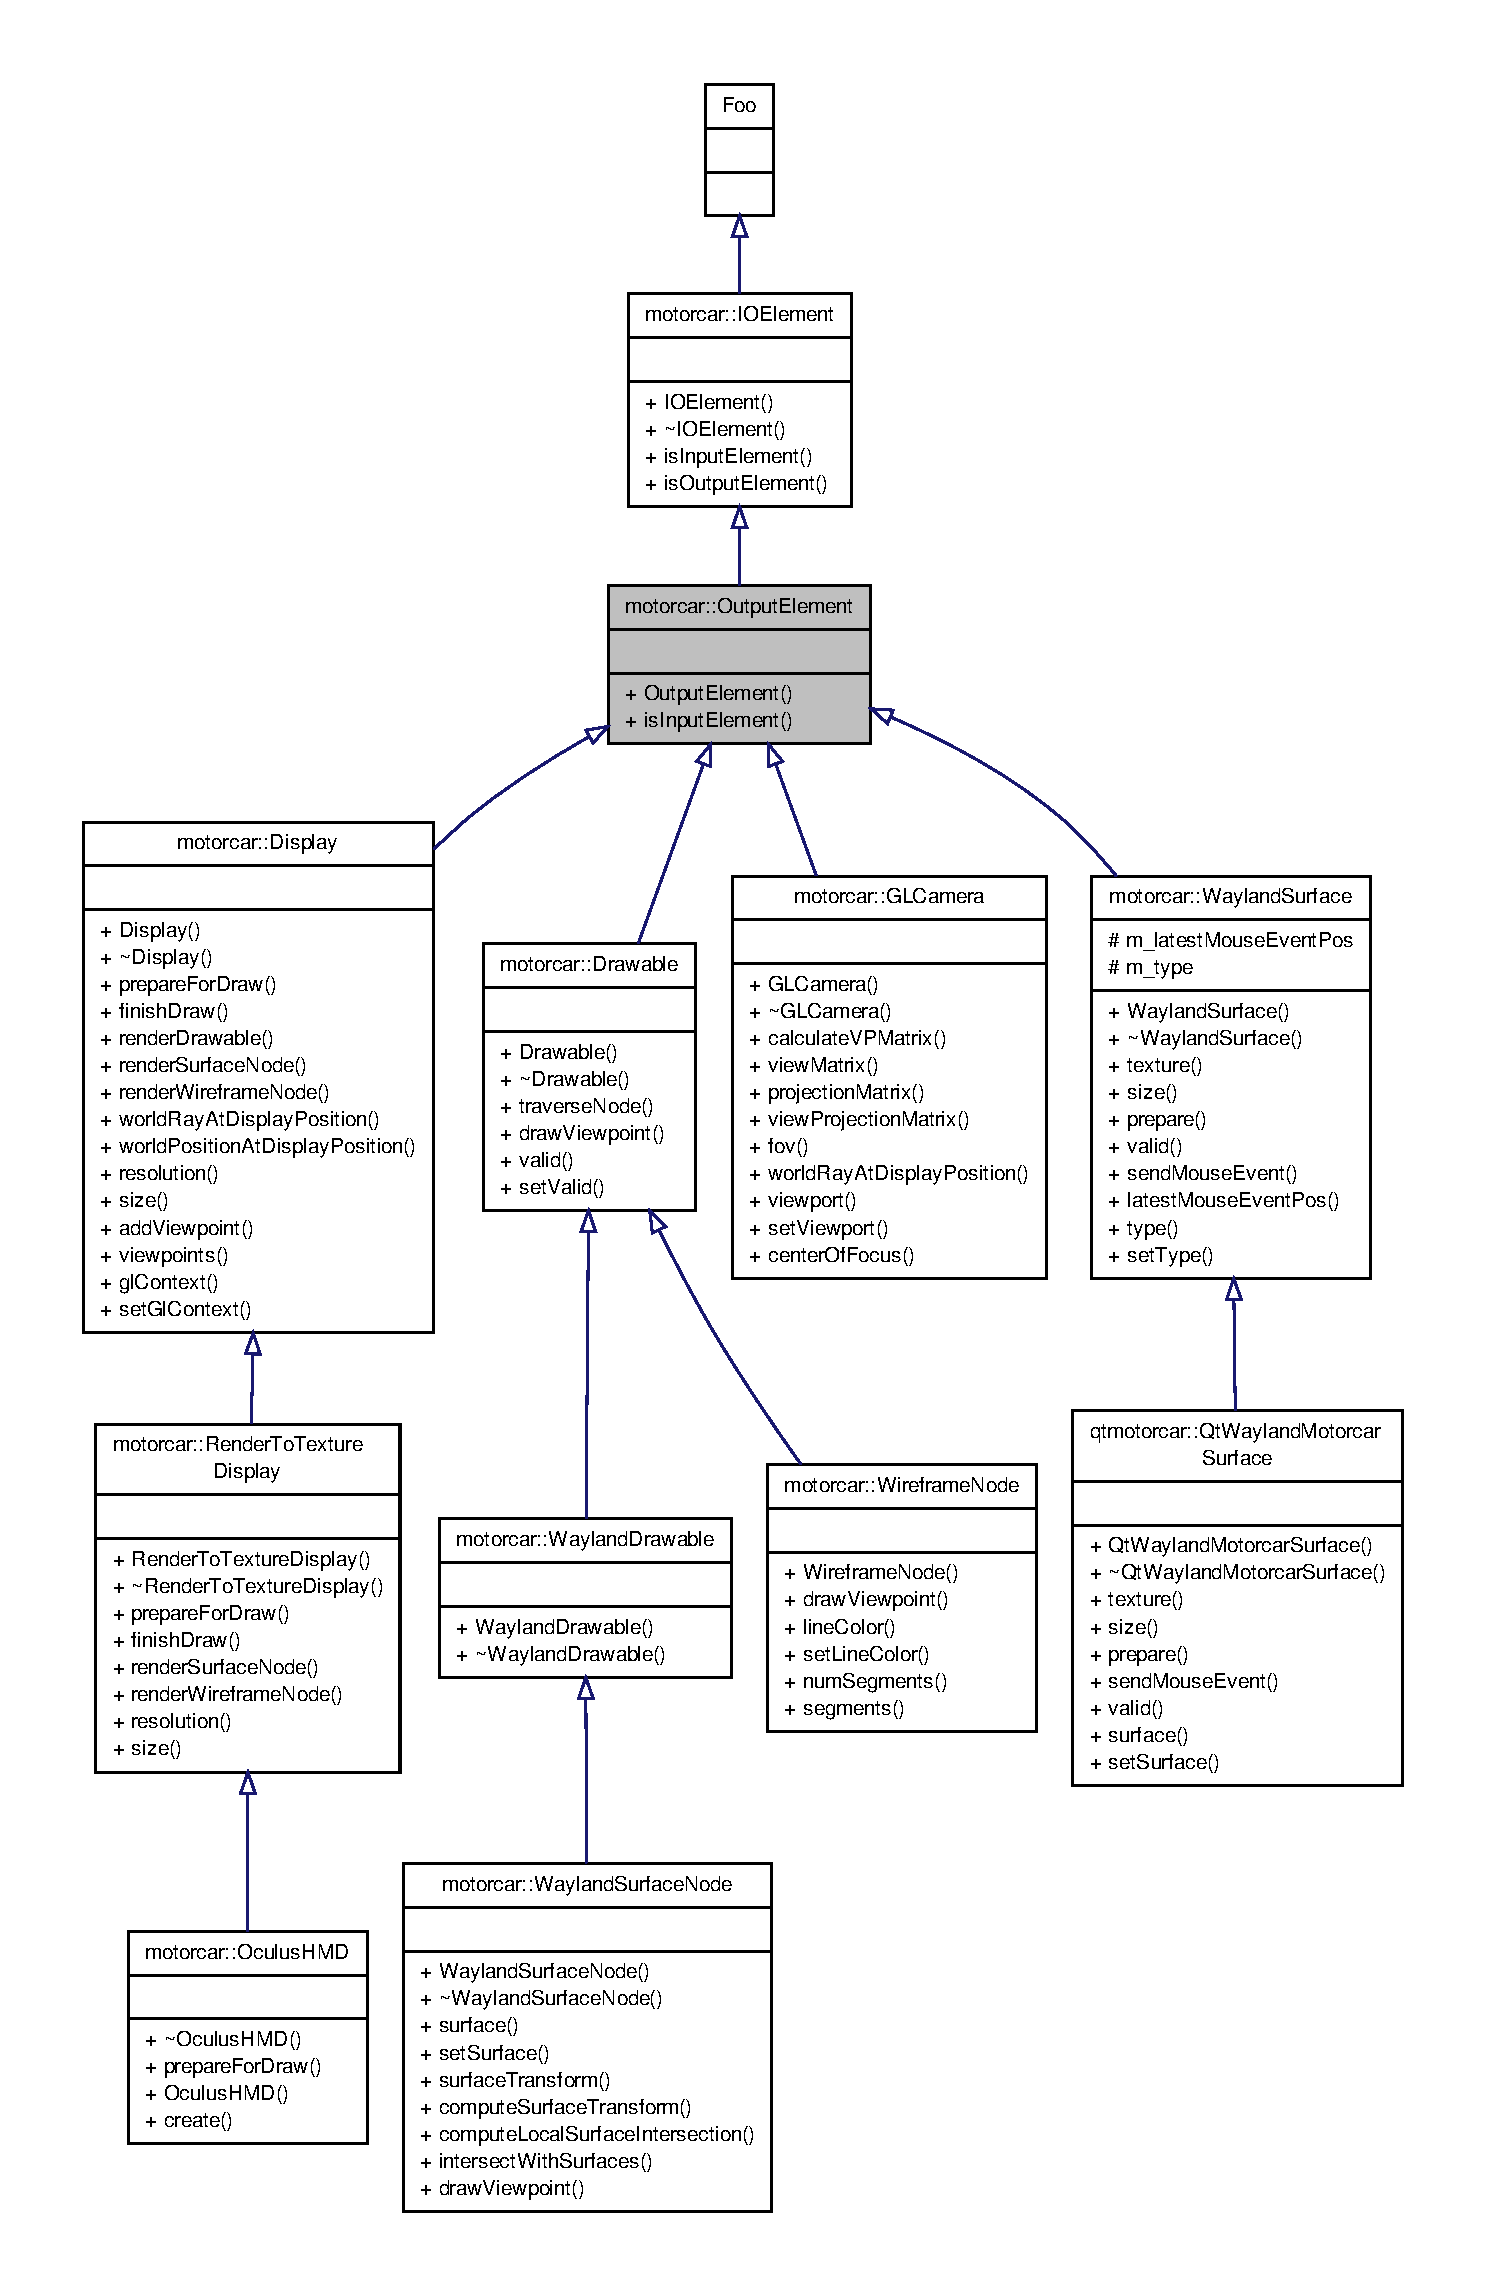
\includegraphics[width=350pt]{classmotorcar_1_1OutputElement__inherit__graph}
\end{center}
\end{figure}


Collaboration diagram for motorcar\-:\-:Output\-Element\-:
\nopagebreak
\begin{figure}[H]
\begin{center}
\leavevmode
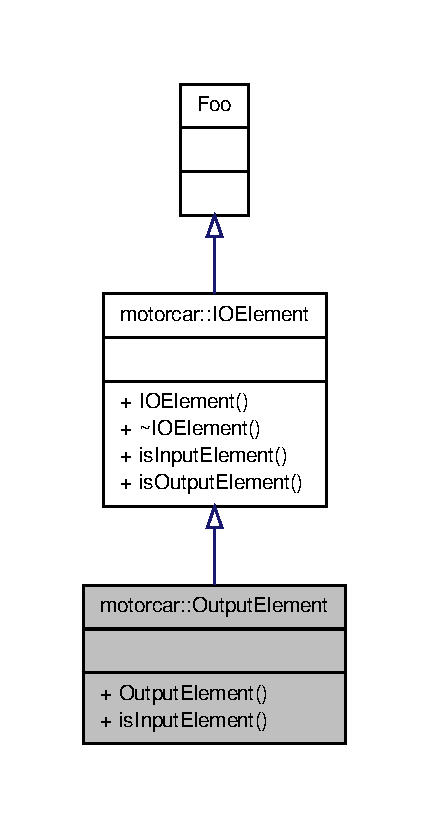
\includegraphics[width=206pt]{classmotorcar_1_1OutputElement__coll__graph}
\end{center}
\end{figure}
\subsection*{Public Member Functions}
\begin{DoxyCompactItemize}
\item 
\hyperlink{classmotorcar_1_1OutputElement_a154f750cf49fa42814bbdab7e2da05b5}{Output\-Element} ()
\item 
bool \hyperlink{classmotorcar_1_1OutputElement_a4edec9c114aabe4adf60fee24e8468de}{is\-Input\-Element} () const 
\end{DoxyCompactItemize}


\subsection{Constructor \& Destructor Documentation}
\hypertarget{classmotorcar_1_1OutputElement_a154f750cf49fa42814bbdab7e2da05b5}{\index{motorcar\-::\-Output\-Element@{motorcar\-::\-Output\-Element}!Output\-Element@{Output\-Element}}
\index{Output\-Element@{Output\-Element}!motorcar::OutputElement@{motorcar\-::\-Output\-Element}}
\subsubsection[{Output\-Element}]{\setlength{\rightskip}{0pt plus 5cm}Output\-Element\-::\-Output\-Element (
\begin{DoxyParamCaption}
{}
\end{DoxyParamCaption}
)}}\label{classmotorcar_1_1OutputElement_a154f750cf49fa42814bbdab7e2da05b5}


\subsection{Member Function Documentation}
\hypertarget{classmotorcar_1_1OutputElement_a4edec9c114aabe4adf60fee24e8468de}{\index{motorcar\-::\-Output\-Element@{motorcar\-::\-Output\-Element}!is\-Input\-Element@{is\-Input\-Element}}
\index{is\-Input\-Element@{is\-Input\-Element}!motorcar::OutputElement@{motorcar\-::\-Output\-Element}}
\subsubsection[{is\-Input\-Element}]{\setlength{\rightskip}{0pt plus 5cm}bool Output\-Element\-::is\-Input\-Element (
\begin{DoxyParamCaption}
{}
\end{DoxyParamCaption}
) const\hspace{0.3cm}{\ttfamily [virtual]}}}\label{classmotorcar_1_1OutputElement_a4edec9c114aabe4adf60fee24e8468de}


Implements \hyperlink{classmotorcar_1_1IOElement_ab73b2687c5452ff694f20c40357ee219}{motorcar\-::\-I\-O\-Element}.



The documentation for this class was generated from the following files\-:\begin{DoxyCompactItemize}
\item 
/home/dave/thesis/qtwayland-\/motorcar-\/compositor/motorcar/src/scenegraph/output/\hyperlink{outputelement_8h}{outputelement.\-h}\item 
/home/dave/thesis/qtwayland-\/motorcar-\/compositor/motorcar/src/scenegraph/output/\hyperlink{outputelement_8cpp}{outputelement.\-cpp}\end{DoxyCompactItemize}

\hypertarget{classmotorcar_1_1PhysicalNode}{\section{motorcar\-:\-:Physical\-Node Class Reference}
\label{classmotorcar_1_1PhysicalNode}\index{motorcar\-::\-Physical\-Node@{motorcar\-::\-Physical\-Node}}
}


{\ttfamily \#include $<$physicalnode.\-h$>$}



Inheritance diagram for motorcar\-:\-:Physical\-Node\-:
\nopagebreak
\begin{figure}[H]
\begin{center}
\leavevmode
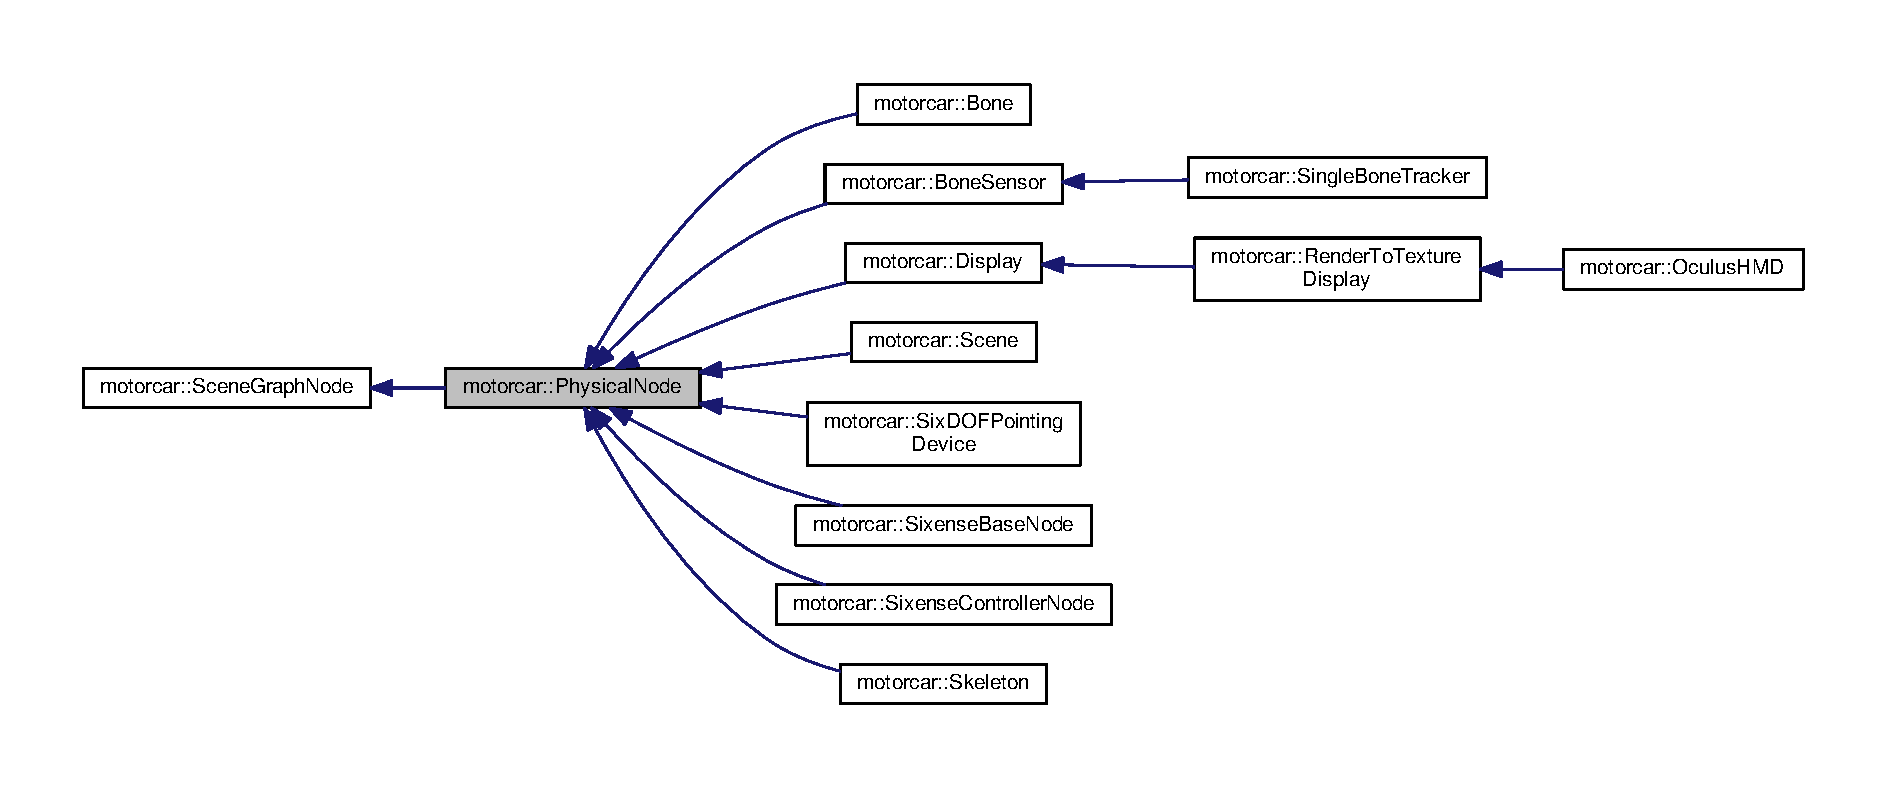
\includegraphics[width=350pt]{classmotorcar_1_1PhysicalNode__inherit__graph}
\end{center}
\end{figure}


Collaboration diagram for motorcar\-:\-:Physical\-Node\-:
\nopagebreak
\begin{figure}[H]
\begin{center}
\leavevmode
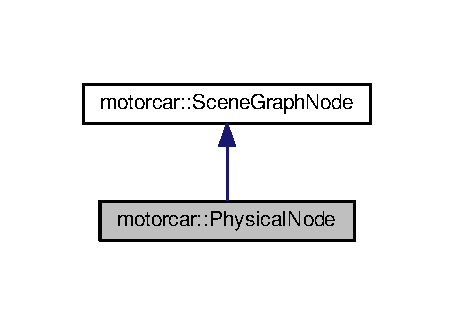
\includegraphics[width=218pt]{classmotorcar_1_1PhysicalNode__coll__graph}
\end{center}
\end{figure}
\subsection*{Public Member Functions}
\begin{DoxyCompactItemize}
\item 
\hyperlink{classmotorcar_1_1PhysicalNode_a91ba5f3ead25d072f128375369b75fe0}{Physical\-Node} (\hyperlink{classmotorcar_1_1PhysicalNode}{Physical\-Node} $\ast$parent, const glm\-::mat4 \&\hyperlink{classmotorcar_1_1SceneGraphNode_ad96e79fdd739ac8223a3128003be391a}{transform}=glm\-::mat4())
\item 
virtual \hyperlink{classmotorcar_1_1PhysicalNode_aa132dbe84a01971eb4e149852a1b52f1}{$\sim$\-Physical\-Node} ()
\item 
void \hyperlink{classmotorcar_1_1PhysicalNode_aadcd6c81c0f8b2f57e6bebe9100d0690}{set\-Parent\-Node} (\hyperlink{classmotorcar_1_1PhysicalNode}{Physical\-Node} $\ast$parent)
\end{DoxyCompactItemize}
\subsection*{Protected Member Functions}
\begin{DoxyCompactItemize}
\item 
\hyperlink{classmotorcar_1_1PhysicalNode_a8194d6949b0886071bda80fb314aabde}{Physical\-Node} ()
\end{DoxyCompactItemize}


\subsection{Constructor \& Destructor Documentation}
\hypertarget{classmotorcar_1_1PhysicalNode_a91ba5f3ead25d072f128375369b75fe0}{\index{motorcar\-::\-Physical\-Node@{motorcar\-::\-Physical\-Node}!Physical\-Node@{Physical\-Node}}
\index{Physical\-Node@{Physical\-Node}!motorcar::PhysicalNode@{motorcar\-::\-Physical\-Node}}
\subsubsection[{Physical\-Node}]{\setlength{\rightskip}{0pt plus 5cm}Physical\-Node\-::\-Physical\-Node (
\begin{DoxyParamCaption}
\item[{{\bf Physical\-Node} $\ast$}]{parent, }
\item[{const glm\-::mat4 \&}]{transform = {\ttfamily glm\-:\-:mat4()}}
\end{DoxyParamCaption}
)}}\label{classmotorcar_1_1PhysicalNode_a91ba5f3ead25d072f128375369b75fe0}
\hypertarget{classmotorcar_1_1PhysicalNode_aa132dbe84a01971eb4e149852a1b52f1}{\index{motorcar\-::\-Physical\-Node@{motorcar\-::\-Physical\-Node}!$\sim$\-Physical\-Node@{$\sim$\-Physical\-Node}}
\index{$\sim$\-Physical\-Node@{$\sim$\-Physical\-Node}!motorcar::PhysicalNode@{motorcar\-::\-Physical\-Node}}
\subsubsection[{$\sim$\-Physical\-Node}]{\setlength{\rightskip}{0pt plus 5cm}virtual motorcar\-::\-Physical\-Node\-::$\sim$\-Physical\-Node (
\begin{DoxyParamCaption}
{}
\end{DoxyParamCaption}
)\hspace{0.3cm}{\ttfamily [inline]}, {\ttfamily [virtual]}}}\label{classmotorcar_1_1PhysicalNode_aa132dbe84a01971eb4e149852a1b52f1}
\hypertarget{classmotorcar_1_1PhysicalNode_a8194d6949b0886071bda80fb314aabde}{\index{motorcar\-::\-Physical\-Node@{motorcar\-::\-Physical\-Node}!Physical\-Node@{Physical\-Node}}
\index{Physical\-Node@{Physical\-Node}!motorcar::PhysicalNode@{motorcar\-::\-Physical\-Node}}
\subsubsection[{Physical\-Node}]{\setlength{\rightskip}{0pt plus 5cm}Physical\-Node\-::\-Physical\-Node (
\begin{DoxyParamCaption}
{}
\end{DoxyParamCaption}
)\hspace{0.3cm}{\ttfamily [protected]}}}\label{classmotorcar_1_1PhysicalNode_a8194d6949b0886071bda80fb314aabde}


\subsection{Member Function Documentation}
\hypertarget{classmotorcar_1_1PhysicalNode_aadcd6c81c0f8b2f57e6bebe9100d0690}{\index{motorcar\-::\-Physical\-Node@{motorcar\-::\-Physical\-Node}!set\-Parent\-Node@{set\-Parent\-Node}}
\index{set\-Parent\-Node@{set\-Parent\-Node}!motorcar::PhysicalNode@{motorcar\-::\-Physical\-Node}}
\subsubsection[{set\-Parent\-Node}]{\setlength{\rightskip}{0pt plus 5cm}void Physical\-Node\-::set\-Parent\-Node (
\begin{DoxyParamCaption}
\item[{{\bf Physical\-Node} $\ast$}]{parent}
\end{DoxyParamCaption}
)}}\label{classmotorcar_1_1PhysicalNode_aadcd6c81c0f8b2f57e6bebe9100d0690}


The documentation for this class was generated from the following files\-:\begin{DoxyCompactItemize}
\item 
/home/dave/thesis/qtwayland-\/motorcar-\/compositor/motorcar/src/scenegraph/\hyperlink{physicalnode_8h}{physicalnode.\-h}\item 
/home/dave/thesis/qtwayland-\/motorcar-\/compositor/motorcar/src/scenegraph/\hyperlink{physicalnode_8cpp}{physicalnode.\-cpp}\end{DoxyCompactItemize}

\hypertarget{structmotorcar_1_1Geometry_1_1Plane}{\section{motorcar\-:\-:Geometry\-:\-:Plane Struct Reference}
\label{structmotorcar_1_1Geometry_1_1Plane}\index{motorcar\-::\-Geometry\-::\-Plane@{motorcar\-::\-Geometry\-::\-Plane}}
}


{\ttfamily \#include $<$geometry.\-h$>$}

\subsection*{Public Member Functions}
\begin{DoxyCompactItemize}
\item 
\hyperlink{structmotorcar_1_1Geometry_1_1Plane_aa50a62c6e979384b4026a1ba81a29c19}{Plane} (glm\-::vec3 \hyperlink{structmotorcar_1_1Geometry_1_1Plane_ad1aa2ffa451147b0fe911f5b78c10500}{p}, glm\-::vec3 \hyperlink{structmotorcar_1_1Geometry_1_1Plane_adc343be1d51473ca22505d7427a7631c}{n})
\item 
float \hyperlink{structmotorcar_1_1Geometry_1_1Plane_a108d18bf80259951130d1b2b7e8bf8ce}{intersect} (\hyperlink{structmotorcar_1_1Geometry_1_1Ray}{Ray} r)
\end{DoxyCompactItemize}
\subsection*{Public Attributes}
\begin{DoxyCompactItemize}
\item 
glm\-::vec3 \hyperlink{structmotorcar_1_1Geometry_1_1Plane_ad1aa2ffa451147b0fe911f5b78c10500}{p}
\item 
glm\-::vec3 \hyperlink{structmotorcar_1_1Geometry_1_1Plane_adc343be1d51473ca22505d7427a7631c}{n}
\end{DoxyCompactItemize}


\subsection{Constructor \& Destructor Documentation}
\hypertarget{structmotorcar_1_1Geometry_1_1Plane_aa50a62c6e979384b4026a1ba81a29c19}{\index{motorcar\-::\-Geometry\-::\-Plane@{motorcar\-::\-Geometry\-::\-Plane}!Plane@{Plane}}
\index{Plane@{Plane}!motorcar::Geometry::Plane@{motorcar\-::\-Geometry\-::\-Plane}}
\subsubsection[{Plane}]{\setlength{\rightskip}{0pt plus 5cm}Geometry\-::\-Plane\-::\-Plane (
\begin{DoxyParamCaption}
\item[{glm\-::vec3}]{p, }
\item[{glm\-::vec3}]{n}
\end{DoxyParamCaption}
)}}\label{structmotorcar_1_1Geometry_1_1Plane_aa50a62c6e979384b4026a1ba81a29c19}


\subsection{Member Function Documentation}
\hypertarget{structmotorcar_1_1Geometry_1_1Plane_a108d18bf80259951130d1b2b7e8bf8ce}{\index{motorcar\-::\-Geometry\-::\-Plane@{motorcar\-::\-Geometry\-::\-Plane}!intersect@{intersect}}
\index{intersect@{intersect}!motorcar::Geometry::Plane@{motorcar\-::\-Geometry\-::\-Plane}}
\subsubsection[{intersect}]{\setlength{\rightskip}{0pt plus 5cm}float Geometry\-::\-Plane\-::intersect (
\begin{DoxyParamCaption}
\item[{{\bf Geometry\-::\-Ray}}]{r}
\end{DoxyParamCaption}
)}}\label{structmotorcar_1_1Geometry_1_1Plane_a108d18bf80259951130d1b2b7e8bf8ce}


\subsection{Member Data Documentation}
\hypertarget{structmotorcar_1_1Geometry_1_1Plane_adc343be1d51473ca22505d7427a7631c}{\index{motorcar\-::\-Geometry\-::\-Plane@{motorcar\-::\-Geometry\-::\-Plane}!n@{n}}
\index{n@{n}!motorcar::Geometry::Plane@{motorcar\-::\-Geometry\-::\-Plane}}
\subsubsection[{n}]{\setlength{\rightskip}{0pt plus 5cm}glm\-::vec3 motorcar\-::\-Geometry\-::\-Plane\-::n}}\label{structmotorcar_1_1Geometry_1_1Plane_adc343be1d51473ca22505d7427a7631c}
\hypertarget{structmotorcar_1_1Geometry_1_1Plane_ad1aa2ffa451147b0fe911f5b78c10500}{\index{motorcar\-::\-Geometry\-::\-Plane@{motorcar\-::\-Geometry\-::\-Plane}!p@{p}}
\index{p@{p}!motorcar::Geometry::Plane@{motorcar\-::\-Geometry\-::\-Plane}}
\subsubsection[{p}]{\setlength{\rightskip}{0pt plus 5cm}glm\-::vec3 motorcar\-::\-Geometry\-::\-Plane\-::p}}\label{structmotorcar_1_1Geometry_1_1Plane_ad1aa2ffa451147b0fe911f5b78c10500}


The documentation for this struct was generated from the following files\-:\begin{DoxyCompactItemize}
\item 
/home/dave/thesis/motorcar/src/compositor/\hyperlink{geometry_8h}{geometry.\-h}\item 
/home/dave/thesis/motorcar/src/compositor/\hyperlink{geometry_8cpp}{geometry.\-cpp}\end{DoxyCompactItemize}

\hypertarget{classQOpenGLWindow}{\section{Q\-Open\-G\-L\-Window Class Reference}
\label{classQOpenGLWindow}\index{Q\-Open\-G\-L\-Window@{Q\-Open\-G\-L\-Window}}
}


{\ttfamily \#include $<$qopenglwindow.\-h$>$}



Inheritance diagram for Q\-Open\-G\-L\-Window\-:
\nopagebreak
\begin{figure}[H]
\begin{center}
\leavevmode
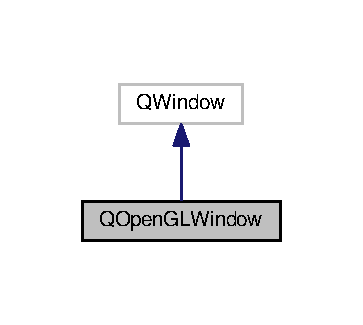
\includegraphics[width=174pt]{classQOpenGLWindow__inherit__graph}
\end{center}
\end{figure}


Collaboration diagram for Q\-Open\-G\-L\-Window\-:
\nopagebreak
\begin{figure}[H]
\begin{center}
\leavevmode
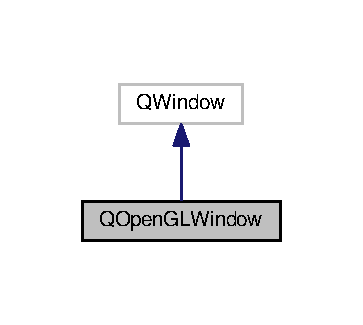
\includegraphics[width=174pt]{classQOpenGLWindow__coll__graph}
\end{center}
\end{figure}
\subsection*{Public Member Functions}
\begin{DoxyCompactItemize}
\item 
\hyperlink{classQOpenGLWindow_a45d1b287e72113aaa653e8e937ebdfd6}{Q\-Open\-G\-L\-Window} (const Q\-Surface\-Format \&format, const Q\-Rect \&\hyperlink{structgeometry}{geometry})
\item 
Q\-Open\-G\-L\-Context $\ast$ \hyperlink{classQOpenGLWindow_ac50866b8a1e723bccea33df6c5a3d1b3}{context} ()
\item 
bool \hyperlink{classQOpenGLWindow_af7602ba08fd50ee8fb9ccbed2d121404}{make\-Current} ()
\item 
void \hyperlink{classQOpenGLWindow_ae8b962ff83b505543adfcd52f4fb203b}{swap\-Buffers} ()
\end{DoxyCompactItemize}
\subsection*{Protected Member Functions}
\begin{DoxyCompactItemize}
\item 
void \hyperlink{classQOpenGLWindow_a60ae6ea64e5efc1a21dea97429ebb838}{touch\-Event} (Q\-Touch\-Event $\ast$event)
\end{DoxyCompactItemize}


\subsection{Constructor \& Destructor Documentation}
\hypertarget{classQOpenGLWindow_a45d1b287e72113aaa653e8e937ebdfd6}{\index{Q\-Open\-G\-L\-Window@{Q\-Open\-G\-L\-Window}!Q\-Open\-G\-L\-Window@{Q\-Open\-G\-L\-Window}}
\index{Q\-Open\-G\-L\-Window@{Q\-Open\-G\-L\-Window}!QOpenGLWindow@{Q\-Open\-G\-L\-Window}}
\subsubsection[{Q\-Open\-G\-L\-Window}]{\setlength{\rightskip}{0pt plus 5cm}Q\-Open\-G\-L\-Window\-::\-Q\-Open\-G\-L\-Window (
\begin{DoxyParamCaption}
\item[{const Q\-Surface\-Format \&}]{format, }
\item[{const Q\-Rect \&}]{geometry}
\end{DoxyParamCaption}
)}}\label{classQOpenGLWindow_a45d1b287e72113aaa653e8e937ebdfd6}


\subsection{Member Function Documentation}
\hypertarget{classQOpenGLWindow_ac50866b8a1e723bccea33df6c5a3d1b3}{\index{Q\-Open\-G\-L\-Window@{Q\-Open\-G\-L\-Window}!context@{context}}
\index{context@{context}!QOpenGLWindow@{Q\-Open\-G\-L\-Window}}
\subsubsection[{context}]{\setlength{\rightskip}{0pt plus 5cm}Q\-Open\-G\-L\-Context$\ast$ Q\-Open\-G\-L\-Window\-::context (
\begin{DoxyParamCaption}
{}
\end{DoxyParamCaption}
)\hspace{0.3cm}{\ttfamily [inline]}}}\label{classQOpenGLWindow_ac50866b8a1e723bccea33df6c5a3d1b3}
\hypertarget{classQOpenGLWindow_af7602ba08fd50ee8fb9ccbed2d121404}{\index{Q\-Open\-G\-L\-Window@{Q\-Open\-G\-L\-Window}!make\-Current@{make\-Current}}
\index{make\-Current@{make\-Current}!QOpenGLWindow@{Q\-Open\-G\-L\-Window}}
\subsubsection[{make\-Current}]{\setlength{\rightskip}{0pt plus 5cm}bool Q\-Open\-G\-L\-Window\-::make\-Current (
\begin{DoxyParamCaption}
{}
\end{DoxyParamCaption}
)\hspace{0.3cm}{\ttfamily [inline]}}}\label{classQOpenGLWindow_af7602ba08fd50ee8fb9ccbed2d121404}
\hypertarget{classQOpenGLWindow_ae8b962ff83b505543adfcd52f4fb203b}{\index{Q\-Open\-G\-L\-Window@{Q\-Open\-G\-L\-Window}!swap\-Buffers@{swap\-Buffers}}
\index{swap\-Buffers@{swap\-Buffers}!QOpenGLWindow@{Q\-Open\-G\-L\-Window}}
\subsubsection[{swap\-Buffers}]{\setlength{\rightskip}{0pt plus 5cm}void Q\-Open\-G\-L\-Window\-::swap\-Buffers (
\begin{DoxyParamCaption}
{}
\end{DoxyParamCaption}
)\hspace{0.3cm}{\ttfamily [inline]}}}\label{classQOpenGLWindow_ae8b962ff83b505543adfcd52f4fb203b}
\hypertarget{classQOpenGLWindow_a60ae6ea64e5efc1a21dea97429ebb838}{\index{Q\-Open\-G\-L\-Window@{Q\-Open\-G\-L\-Window}!touch\-Event@{touch\-Event}}
\index{touch\-Event@{touch\-Event}!QOpenGLWindow@{Q\-Open\-G\-L\-Window}}
\subsubsection[{touch\-Event}]{\setlength{\rightskip}{0pt plus 5cm}void Q\-Open\-G\-L\-Window\-::touch\-Event (
\begin{DoxyParamCaption}
\item[{Q\-Touch\-Event $\ast$}]{event}
\end{DoxyParamCaption}
)\hspace{0.3cm}{\ttfamily [protected]}}}\label{classQOpenGLWindow_a60ae6ea64e5efc1a21dea97429ebb838}


The documentation for this class was generated from the following files\-:\begin{DoxyCompactItemize}
\item 
/home/dave/thesis/motorcar/src/compositor/qt/\hyperlink{qopenglwindow_8h}{qopenglwindow.\-h}\item 
/home/dave/thesis/motorcar/src/compositor/qt/\hyperlink{qopenglwindow_8cpp}{qopenglwindow.\-cpp}\end{DoxyCompactItemize}

\hypertarget{classqtmotorcar_1_1QtWaylandMotorcarCompositor}{\section{qtmotorcar\-:\-:Qt\-Wayland\-Motorcar\-Compositor Class Reference}
\label{classqtmotorcar_1_1QtWaylandMotorcarCompositor}\index{qtmotorcar\-::\-Qt\-Wayland\-Motorcar\-Compositor@{qtmotorcar\-::\-Qt\-Wayland\-Motorcar\-Compositor}}
}


{\ttfamily \#include $<$qtwaylandmotorcarcompositor.\-h$>$}



Inheritance diagram for qtmotorcar\-:\-:Qt\-Wayland\-Motorcar\-Compositor\-:
\nopagebreak
\begin{figure}[H]
\begin{center}
\leavevmode
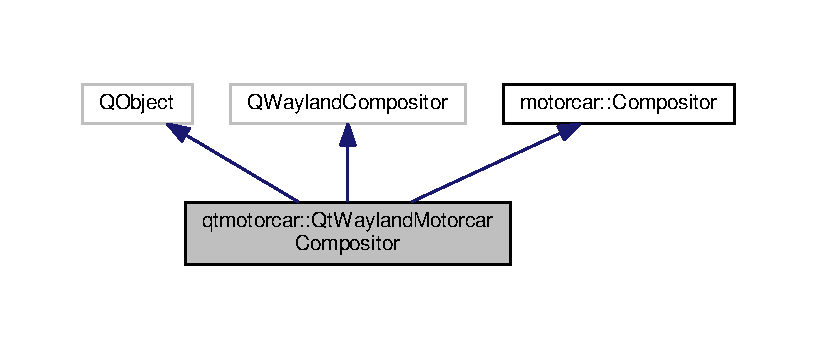
\includegraphics[width=350pt]{classqtmotorcar_1_1QtWaylandMotorcarCompositor__inherit__graph}
\end{center}
\end{figure}


Collaboration diagram for qtmotorcar\-:\-:Qt\-Wayland\-Motorcar\-Compositor\-:
\nopagebreak
\begin{figure}[H]
\begin{center}
\leavevmode
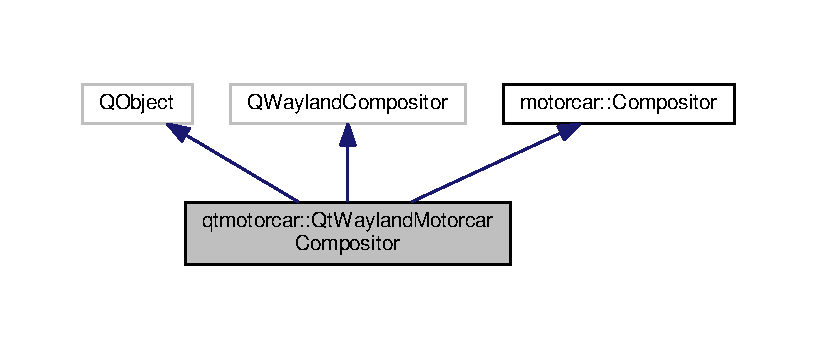
\includegraphics[width=350pt]{classqtmotorcar_1_1QtWaylandMotorcarCompositor__coll__graph}
\end{center}
\end{figure}
\subsection*{Public Member Functions}
\begin{DoxyCompactItemize}
\item 
\hyperlink{classqtmotorcar_1_1QtWaylandMotorcarCompositor_a0de2ac0cbe6d725a501375a84573c470}{Qt\-Wayland\-Motorcar\-Compositor} (\hyperlink{classQOpenGLWindow}{Q\-Open\-G\-L\-Window} $\ast$\hyperlink{structwindow}{window}, Q\-Gui\-Application $\ast$app, \hyperlink{classmotorcar_1_1Scene}{motorcar\-::\-Scene} $\ast$\hyperlink{classqtmotorcar_1_1QtWaylandMotorcarCompositor_a8bb6c8e6a7acad99b814b192534f3ee2}{scene})
\item 
\hyperlink{classqtmotorcar_1_1QtWaylandMotorcarCompositor_a8d0178c57bdbe03ef7e4db6e13900950}{$\sim$\-Qt\-Wayland\-Motorcar\-Compositor} ()
\item 
virtual int \hyperlink{classqtmotorcar_1_1QtWaylandMotorcarCompositor_a34cd3f4acc535584eb066d3fe32ed9bf}{start} () override
\begin{DoxyCompactList}\small\item\em starts the compositor main draw loop \end{DoxyCompactList}\item 
virtual \hyperlink{classmotorcar_1_1OpenGLContext}{motorcar\-::\-Open\-G\-L\-Context} $\ast$ \hyperlink{classqtmotorcar_1_1QtWaylandMotorcarCompositor_a1fb6e9d59011be2912bc9cf51496b191}{get\-Context} () override
\begin{DoxyCompactList}\small\item\em gets the Open\-G\-L context in which the compositing is taking place \end{DoxyCompactList}\item 
struct wl\-\_\-display $\ast$ \hyperlink{classqtmotorcar_1_1QtWaylandMotorcarCompositor_a9e29a67d95d6aa74a08b2a3deed19dfe}{wl\-Display} () override
\item 
\hyperlink{classmotorcar_1_1WaylandSurface}{motorcar\-::\-Wayland\-Surface} $\ast$ \hyperlink{classqtmotorcar_1_1QtWaylandMotorcarCompositor_ad4262e2dce170d25080e5c205fecc5ca}{get\-Surface\-From\-Resource} (struct wl\-\_\-resource $\ast$resource) override
\item 
\hyperlink{classOpenGLData}{Open\-G\-L\-Data} $\ast$ \hyperlink{classqtmotorcar_1_1QtWaylandMotorcarCompositor_a50bc0b510d20d0298b9e164804543f81}{gl\-Data} () const 
\item 
void \hyperlink{classqtmotorcar_1_1QtWaylandMotorcarCompositor_a0122a32ec769e7190b3a2e0a838f0053}{set\-Gl\-Data} (\hyperlink{classOpenGLData}{Open\-G\-L\-Data} $\ast$\hyperlink{classqtmotorcar_1_1QtWaylandMotorcarCompositor_a50bc0b510d20d0298b9e164804543f81}{gl\-Data})
\item 
\hyperlink{classmotorcar_1_1Scene}{motorcar\-::\-Scene} $\ast$ \hyperlink{classqtmotorcar_1_1QtWaylandMotorcarCompositor_a8bb6c8e6a7acad99b814b192534f3ee2}{scene} () const 
\item 
void \hyperlink{classqtmotorcar_1_1QtWaylandMotorcarCompositor_a2a896748e415515de155c22ef70adeb0}{set\-Scene} (\hyperlink{classmotorcar_1_1Scene}{motorcar\-::\-Scene} $\ast$\hyperlink{classqtmotorcar_1_1QtWaylandMotorcarCompositor_a8bb6c8e6a7acad99b814b192534f3ee2}{scene})
\item 
\hyperlink{classqtmotorcar_1_1QtWaylandMotorcarSurface}{Qt\-Wayland\-Motorcar\-Surface} $\ast$ \hyperlink{classqtmotorcar_1_1QtWaylandMotorcarCompositor_a97c4d656c14bd2b6877405d5003fb741}{get\-Motorcar\-Surface} (Q\-Wayland\-Surface $\ast$\hyperlink{simple-egl_8c_a0720952aa1caded45b5bcdce589663a9}{surface}=N\-U\-L\-L) const 
\item 
\hyperlink{classqtmotorcar_1_1QtWaylandMotorcarSeat}{Qt\-Wayland\-Motorcar\-Seat} $\ast$ \hyperlink{classqtmotorcar_1_1QtWaylandMotorcarCompositor_a6104791cebeec6529ec784db17096a38}{default\-Seat} () const 
\item 
void \hyperlink{classqtmotorcar_1_1QtWaylandMotorcarCompositor_a6ea6591a5e3999156f7418f8a61db992}{set\-Default\-Seat} (\hyperlink{classqtmotorcar_1_1QtWaylandMotorcarSeat}{Qt\-Wayland\-Motorcar\-Seat} $\ast$\hyperlink{classqtmotorcar_1_1QtWaylandMotorcarCompositor_a6104791cebeec6529ec784db17096a38}{default\-Seat})
\end{DoxyCompactItemize}
\subsection*{Static Public Member Functions}
\begin{DoxyCompactItemize}
\item 
static \\*
\hyperlink{classqtmotorcar_1_1QtWaylandMotorcarCompositor}{Qt\-Wayland\-Motorcar\-Compositor} $\ast$ \hyperlink{classqtmotorcar_1_1QtWaylandMotorcarCompositor_a169e428e534906108290bb5c4512ca13}{create} (int argc, char $\ast$$\ast$argv, \hyperlink{classmotorcar_1_1Scene}{motorcar\-::\-Scene} $\ast$\hyperlink{classqtmotorcar_1_1QtWaylandMotorcarCompositor_a8bb6c8e6a7acad99b814b192534f3ee2}{scene})
\end{DoxyCompactItemize}
\subsection*{Protected Member Functions}
\begin{DoxyCompactItemize}
\item 
void \hyperlink{classqtmotorcar_1_1QtWaylandMotorcarCompositor_a12ce718691bc19318acd23b981a72cb8}{surface\-Damaged} (Q\-Wayland\-Surface $\ast$\hyperlink{simple-egl_8c_a0720952aa1caded45b5bcdce589663a9}{surface})
\item 
void \hyperlink{classqtmotorcar_1_1QtWaylandMotorcarCompositor_a4bda9a0989cb8c22e7b5d1a687763b61}{surface\-Created} (Q\-Wayland\-Surface $\ast$\hyperlink{simple-egl_8c_a0720952aa1caded45b5bcdce589663a9}{surface})
\item 
Q\-Wayland\-Surface $\ast$ \hyperlink{classqtmotorcar_1_1QtWaylandMotorcarCompositor_adcc9307301b665c9d5ccea73fef01453}{surface\-At} (const Q\-Point\-F \&point, Q\-Point\-F $\ast$local=0)
\item 
bool \hyperlink{classqtmotorcar_1_1QtWaylandMotorcarCompositor_a1d5c76d5c4dfd029d90803d889c07206}{event\-Filter} (Q\-Object $\ast$obj, Q\-Event $\ast$event)
\item 
Q\-Point\-F \hyperlink{classqtmotorcar_1_1QtWaylandMotorcarCompositor_af3c3c2e2dbfd18427c8b38f83f0fa01f}{to\-Surface} (Q\-Wayland\-Surface $\ast$\hyperlink{simple-egl_8c_a0720952aa1caded45b5bcdce589663a9}{surface}, const Q\-Point\-F \&point) const 
\item 
void \hyperlink{classqtmotorcar_1_1QtWaylandMotorcarCompositor_a4555fa6ed0c867668fe735d9192331c7}{set\-Cursor\-Surface} (Q\-Wayland\-Surface $\ast$\hyperlink{simple-egl_8c_a0720952aa1caded45b5bcdce589663a9}{surface}, int hotspot\-X, int hotspot\-Y)
\item 
void \hyperlink{classqtmotorcar_1_1QtWaylandMotorcarCompositor_ac2210c9eaefdc154eac4111807232eb0}{ensure\-Keyboard\-Focus\-Surface} (Q\-Wayland\-Surface $\ast$old\-Surface)
\end{DoxyCompactItemize}


\subsection{Constructor \& Destructor Documentation}
\hypertarget{classqtmotorcar_1_1QtWaylandMotorcarCompositor_a0de2ac0cbe6d725a501375a84573c470}{\index{qtmotorcar\-::\-Qt\-Wayland\-Motorcar\-Compositor@{qtmotorcar\-::\-Qt\-Wayland\-Motorcar\-Compositor}!Qt\-Wayland\-Motorcar\-Compositor@{Qt\-Wayland\-Motorcar\-Compositor}}
\index{Qt\-Wayland\-Motorcar\-Compositor@{Qt\-Wayland\-Motorcar\-Compositor}!qtmotorcar::QtWaylandMotorcarCompositor@{qtmotorcar\-::\-Qt\-Wayland\-Motorcar\-Compositor}}
\subsubsection[{Qt\-Wayland\-Motorcar\-Compositor}]{\setlength{\rightskip}{0pt plus 5cm}Qt\-Wayland\-Motorcar\-Compositor\-::\-Qt\-Wayland\-Motorcar\-Compositor (
\begin{DoxyParamCaption}
\item[{{\bf Q\-Open\-G\-L\-Window} $\ast$}]{window, }
\item[{Q\-Gui\-Application $\ast$}]{app, }
\item[{{\bf motorcar\-::\-Scene} $\ast$}]{scene}
\end{DoxyParamCaption}
)}}\label{classqtmotorcar_1_1QtWaylandMotorcarCompositor_a0de2ac0cbe6d725a501375a84573c470}
\hypertarget{classqtmotorcar_1_1QtWaylandMotorcarCompositor_a8d0178c57bdbe03ef7e4db6e13900950}{\index{qtmotorcar\-::\-Qt\-Wayland\-Motorcar\-Compositor@{qtmotorcar\-::\-Qt\-Wayland\-Motorcar\-Compositor}!$\sim$\-Qt\-Wayland\-Motorcar\-Compositor@{$\sim$\-Qt\-Wayland\-Motorcar\-Compositor}}
\index{$\sim$\-Qt\-Wayland\-Motorcar\-Compositor@{$\sim$\-Qt\-Wayland\-Motorcar\-Compositor}!qtmotorcar::QtWaylandMotorcarCompositor@{qtmotorcar\-::\-Qt\-Wayland\-Motorcar\-Compositor}}
\subsubsection[{$\sim$\-Qt\-Wayland\-Motorcar\-Compositor}]{\setlength{\rightskip}{0pt plus 5cm}Qt\-Wayland\-Motorcar\-Compositor\-::$\sim$\-Qt\-Wayland\-Motorcar\-Compositor (
\begin{DoxyParamCaption}
{}
\end{DoxyParamCaption}
)}}\label{classqtmotorcar_1_1QtWaylandMotorcarCompositor_a8d0178c57bdbe03ef7e4db6e13900950}


\subsection{Member Function Documentation}
\hypertarget{classqtmotorcar_1_1QtWaylandMotorcarCompositor_a169e428e534906108290bb5c4512ca13}{\index{qtmotorcar\-::\-Qt\-Wayland\-Motorcar\-Compositor@{qtmotorcar\-::\-Qt\-Wayland\-Motorcar\-Compositor}!create@{create}}
\index{create@{create}!qtmotorcar::QtWaylandMotorcarCompositor@{qtmotorcar\-::\-Qt\-Wayland\-Motorcar\-Compositor}}
\subsubsection[{create}]{\setlength{\rightskip}{0pt plus 5cm}{\bf Qt\-Wayland\-Motorcar\-Compositor} $\ast$ Qt\-Wayland\-Motorcar\-Compositor\-::create (
\begin{DoxyParamCaption}
\item[{int}]{argc, }
\item[{char $\ast$$\ast$}]{argv, }
\item[{{\bf motorcar\-::\-Scene} $\ast$}]{scene}
\end{DoxyParamCaption}
)\hspace{0.3cm}{\ttfamily [static]}}}\label{classqtmotorcar_1_1QtWaylandMotorcarCompositor_a169e428e534906108290bb5c4512ca13}
\hypertarget{classqtmotorcar_1_1QtWaylandMotorcarCompositor_a6104791cebeec6529ec784db17096a38}{\index{qtmotorcar\-::\-Qt\-Wayland\-Motorcar\-Compositor@{qtmotorcar\-::\-Qt\-Wayland\-Motorcar\-Compositor}!default\-Seat@{default\-Seat}}
\index{default\-Seat@{default\-Seat}!qtmotorcar::QtWaylandMotorcarCompositor@{qtmotorcar\-::\-Qt\-Wayland\-Motorcar\-Compositor}}
\subsubsection[{default\-Seat}]{\setlength{\rightskip}{0pt plus 5cm}{\bf Qt\-Wayland\-Motorcar\-Seat} $\ast$ Qt\-Wayland\-Motorcar\-Compositor\-::default\-Seat (
\begin{DoxyParamCaption}
{}
\end{DoxyParamCaption}
) const}}\label{classqtmotorcar_1_1QtWaylandMotorcarCompositor_a6104791cebeec6529ec784db17096a38}
\hypertarget{classqtmotorcar_1_1QtWaylandMotorcarCompositor_ac2210c9eaefdc154eac4111807232eb0}{\index{qtmotorcar\-::\-Qt\-Wayland\-Motorcar\-Compositor@{qtmotorcar\-::\-Qt\-Wayland\-Motorcar\-Compositor}!ensure\-Keyboard\-Focus\-Surface@{ensure\-Keyboard\-Focus\-Surface}}
\index{ensure\-Keyboard\-Focus\-Surface@{ensure\-Keyboard\-Focus\-Surface}!qtmotorcar::QtWaylandMotorcarCompositor@{qtmotorcar\-::\-Qt\-Wayland\-Motorcar\-Compositor}}
\subsubsection[{ensure\-Keyboard\-Focus\-Surface}]{\setlength{\rightskip}{0pt plus 5cm}void Qt\-Wayland\-Motorcar\-Compositor\-::ensure\-Keyboard\-Focus\-Surface (
\begin{DoxyParamCaption}
\item[{Q\-Wayland\-Surface $\ast$}]{old\-Surface}
\end{DoxyParamCaption}
)\hspace{0.3cm}{\ttfamily [protected]}}}\label{classqtmotorcar_1_1QtWaylandMotorcarCompositor_ac2210c9eaefdc154eac4111807232eb0}
\hypertarget{classqtmotorcar_1_1QtWaylandMotorcarCompositor_a1d5c76d5c4dfd029d90803d889c07206}{\index{qtmotorcar\-::\-Qt\-Wayland\-Motorcar\-Compositor@{qtmotorcar\-::\-Qt\-Wayland\-Motorcar\-Compositor}!event\-Filter@{event\-Filter}}
\index{event\-Filter@{event\-Filter}!qtmotorcar::QtWaylandMotorcarCompositor@{qtmotorcar\-::\-Qt\-Wayland\-Motorcar\-Compositor}}
\subsubsection[{event\-Filter}]{\setlength{\rightskip}{0pt plus 5cm}bool Qt\-Wayland\-Motorcar\-Compositor\-::event\-Filter (
\begin{DoxyParamCaption}
\item[{Q\-Object $\ast$}]{obj, }
\item[{Q\-Event $\ast$}]{event}
\end{DoxyParamCaption}
)\hspace{0.3cm}{\ttfamily [protected]}}}\label{classqtmotorcar_1_1QtWaylandMotorcarCompositor_a1d5c76d5c4dfd029d90803d889c07206}
\hypertarget{classqtmotorcar_1_1QtWaylandMotorcarCompositor_a1fb6e9d59011be2912bc9cf51496b191}{\index{qtmotorcar\-::\-Qt\-Wayland\-Motorcar\-Compositor@{qtmotorcar\-::\-Qt\-Wayland\-Motorcar\-Compositor}!get\-Context@{get\-Context}}
\index{get\-Context@{get\-Context}!qtmotorcar::QtWaylandMotorcarCompositor@{qtmotorcar\-::\-Qt\-Wayland\-Motorcar\-Compositor}}
\subsubsection[{get\-Context}]{\setlength{\rightskip}{0pt plus 5cm}{\bf motorcar\-::\-Open\-G\-L\-Context} $\ast$ Qt\-Wayland\-Motorcar\-Compositor\-::get\-Context (
\begin{DoxyParamCaption}
{}
\end{DoxyParamCaption}
)\hspace{0.3cm}{\ttfamily [override]}, {\ttfamily [virtual]}}}\label{classqtmotorcar_1_1QtWaylandMotorcarCompositor_a1fb6e9d59011be2912bc9cf51496b191}


gets the Open\-G\-L context in which the compositing is taking place 



Implements \hyperlink{classmotorcar_1_1Compositor_afb0a16529f65b5e2ecf8f15524680c57}{motorcar\-::\-Compositor}.

\hypertarget{classqtmotorcar_1_1QtWaylandMotorcarCompositor_a97c4d656c14bd2b6877405d5003fb741}{\index{qtmotorcar\-::\-Qt\-Wayland\-Motorcar\-Compositor@{qtmotorcar\-::\-Qt\-Wayland\-Motorcar\-Compositor}!get\-Motorcar\-Surface@{get\-Motorcar\-Surface}}
\index{get\-Motorcar\-Surface@{get\-Motorcar\-Surface}!qtmotorcar::QtWaylandMotorcarCompositor@{qtmotorcar\-::\-Qt\-Wayland\-Motorcar\-Compositor}}
\subsubsection[{get\-Motorcar\-Surface}]{\setlength{\rightskip}{0pt plus 5cm}{\bf Qt\-Wayland\-Motorcar\-Surface} $\ast$ Qt\-Wayland\-Motorcar\-Compositor\-::get\-Motorcar\-Surface (
\begin{DoxyParamCaption}
\item[{Q\-Wayland\-Surface $\ast$}]{surface = {\ttfamily NULL}}
\end{DoxyParamCaption}
) const}}\label{classqtmotorcar_1_1QtWaylandMotorcarCompositor_a97c4d656c14bd2b6877405d5003fb741}
\hypertarget{classqtmotorcar_1_1QtWaylandMotorcarCompositor_ad4262e2dce170d25080e5c205fecc5ca}{\index{qtmotorcar\-::\-Qt\-Wayland\-Motorcar\-Compositor@{qtmotorcar\-::\-Qt\-Wayland\-Motorcar\-Compositor}!get\-Surface\-From\-Resource@{get\-Surface\-From\-Resource}}
\index{get\-Surface\-From\-Resource@{get\-Surface\-From\-Resource}!qtmotorcar::QtWaylandMotorcarCompositor@{qtmotorcar\-::\-Qt\-Wayland\-Motorcar\-Compositor}}
\subsubsection[{get\-Surface\-From\-Resource}]{\setlength{\rightskip}{0pt plus 5cm}{\bf motorcar\-::\-Wayland\-Surface} $\ast$ Qt\-Wayland\-Motorcar\-Compositor\-::get\-Surface\-From\-Resource (
\begin{DoxyParamCaption}
\item[{struct wl\-\_\-resource $\ast$}]{resource}
\end{DoxyParamCaption}
)\hspace{0.3cm}{\ttfamily [override]}, {\ttfamily [virtual]}}}\label{classqtmotorcar_1_1QtWaylandMotorcarCompositor_ad4262e2dce170d25080e5c205fecc5ca}


Implements \hyperlink{classmotorcar_1_1Compositor_abc7e49b58794334e99a0433389a39929}{motorcar\-::\-Compositor}.

\hypertarget{classqtmotorcar_1_1QtWaylandMotorcarCompositor_a50bc0b510d20d0298b9e164804543f81}{\index{qtmotorcar\-::\-Qt\-Wayland\-Motorcar\-Compositor@{qtmotorcar\-::\-Qt\-Wayland\-Motorcar\-Compositor}!gl\-Data@{gl\-Data}}
\index{gl\-Data@{gl\-Data}!qtmotorcar::QtWaylandMotorcarCompositor@{qtmotorcar\-::\-Qt\-Wayland\-Motorcar\-Compositor}}
\subsubsection[{gl\-Data}]{\setlength{\rightskip}{0pt plus 5cm}{\bf Open\-G\-L\-Data} $\ast$ Qt\-Wayland\-Motorcar\-Compositor\-::gl\-Data (
\begin{DoxyParamCaption}
{}
\end{DoxyParamCaption}
) const}}\label{classqtmotorcar_1_1QtWaylandMotorcarCompositor_a50bc0b510d20d0298b9e164804543f81}
\hypertarget{classqtmotorcar_1_1QtWaylandMotorcarCompositor_a8bb6c8e6a7acad99b814b192534f3ee2}{\index{qtmotorcar\-::\-Qt\-Wayland\-Motorcar\-Compositor@{qtmotorcar\-::\-Qt\-Wayland\-Motorcar\-Compositor}!scene@{scene}}
\index{scene@{scene}!qtmotorcar::QtWaylandMotorcarCompositor@{qtmotorcar\-::\-Qt\-Wayland\-Motorcar\-Compositor}}
\subsubsection[{scene}]{\setlength{\rightskip}{0pt plus 5cm}{\bf motorcar\-::\-Scene} $\ast$ Qt\-Wayland\-Motorcar\-Compositor\-::scene (
\begin{DoxyParamCaption}
{}
\end{DoxyParamCaption}
) const}}\label{classqtmotorcar_1_1QtWaylandMotorcarCompositor_a8bb6c8e6a7acad99b814b192534f3ee2}
\hypertarget{classqtmotorcar_1_1QtWaylandMotorcarCompositor_a4555fa6ed0c867668fe735d9192331c7}{\index{qtmotorcar\-::\-Qt\-Wayland\-Motorcar\-Compositor@{qtmotorcar\-::\-Qt\-Wayland\-Motorcar\-Compositor}!set\-Cursor\-Surface@{set\-Cursor\-Surface}}
\index{set\-Cursor\-Surface@{set\-Cursor\-Surface}!qtmotorcar::QtWaylandMotorcarCompositor@{qtmotorcar\-::\-Qt\-Wayland\-Motorcar\-Compositor}}
\subsubsection[{set\-Cursor\-Surface}]{\setlength{\rightskip}{0pt plus 5cm}void Qt\-Wayland\-Motorcar\-Compositor\-::set\-Cursor\-Surface (
\begin{DoxyParamCaption}
\item[{Q\-Wayland\-Surface $\ast$}]{surface, }
\item[{int}]{hotspot\-X, }
\item[{int}]{hotspot\-Y}
\end{DoxyParamCaption}
)\hspace{0.3cm}{\ttfamily [protected]}}}\label{classqtmotorcar_1_1QtWaylandMotorcarCompositor_a4555fa6ed0c867668fe735d9192331c7}
\hypertarget{classqtmotorcar_1_1QtWaylandMotorcarCompositor_a6ea6591a5e3999156f7418f8a61db992}{\index{qtmotorcar\-::\-Qt\-Wayland\-Motorcar\-Compositor@{qtmotorcar\-::\-Qt\-Wayland\-Motorcar\-Compositor}!set\-Default\-Seat@{set\-Default\-Seat}}
\index{set\-Default\-Seat@{set\-Default\-Seat}!qtmotorcar::QtWaylandMotorcarCompositor@{qtmotorcar\-::\-Qt\-Wayland\-Motorcar\-Compositor}}
\subsubsection[{set\-Default\-Seat}]{\setlength{\rightskip}{0pt plus 5cm}void Qt\-Wayland\-Motorcar\-Compositor\-::set\-Default\-Seat (
\begin{DoxyParamCaption}
\item[{{\bf Qt\-Wayland\-Motorcar\-Seat} $\ast$}]{default\-Seat}
\end{DoxyParamCaption}
)}}\label{classqtmotorcar_1_1QtWaylandMotorcarCompositor_a6ea6591a5e3999156f7418f8a61db992}
\hypertarget{classqtmotorcar_1_1QtWaylandMotorcarCompositor_a0122a32ec769e7190b3a2e0a838f0053}{\index{qtmotorcar\-::\-Qt\-Wayland\-Motorcar\-Compositor@{qtmotorcar\-::\-Qt\-Wayland\-Motorcar\-Compositor}!set\-Gl\-Data@{set\-Gl\-Data}}
\index{set\-Gl\-Data@{set\-Gl\-Data}!qtmotorcar::QtWaylandMotorcarCompositor@{qtmotorcar\-::\-Qt\-Wayland\-Motorcar\-Compositor}}
\subsubsection[{set\-Gl\-Data}]{\setlength{\rightskip}{0pt plus 5cm}void Qt\-Wayland\-Motorcar\-Compositor\-::set\-Gl\-Data (
\begin{DoxyParamCaption}
\item[{{\bf Open\-G\-L\-Data} $\ast$}]{gl\-Data}
\end{DoxyParamCaption}
)}}\label{classqtmotorcar_1_1QtWaylandMotorcarCompositor_a0122a32ec769e7190b3a2e0a838f0053}
\hypertarget{classqtmotorcar_1_1QtWaylandMotorcarCompositor_a2a896748e415515de155c22ef70adeb0}{\index{qtmotorcar\-::\-Qt\-Wayland\-Motorcar\-Compositor@{qtmotorcar\-::\-Qt\-Wayland\-Motorcar\-Compositor}!set\-Scene@{set\-Scene}}
\index{set\-Scene@{set\-Scene}!qtmotorcar::QtWaylandMotorcarCompositor@{qtmotorcar\-::\-Qt\-Wayland\-Motorcar\-Compositor}}
\subsubsection[{set\-Scene}]{\setlength{\rightskip}{0pt plus 5cm}void Qt\-Wayland\-Motorcar\-Compositor\-::set\-Scene (
\begin{DoxyParamCaption}
\item[{{\bf motorcar\-::\-Scene} $\ast$}]{scene}
\end{DoxyParamCaption}
)}}\label{classqtmotorcar_1_1QtWaylandMotorcarCompositor_a2a896748e415515de155c22ef70adeb0}
\hypertarget{classqtmotorcar_1_1QtWaylandMotorcarCompositor_a34cd3f4acc535584eb066d3fe32ed9bf}{\index{qtmotorcar\-::\-Qt\-Wayland\-Motorcar\-Compositor@{qtmotorcar\-::\-Qt\-Wayland\-Motorcar\-Compositor}!start@{start}}
\index{start@{start}!qtmotorcar::QtWaylandMotorcarCompositor@{qtmotorcar\-::\-Qt\-Wayland\-Motorcar\-Compositor}}
\subsubsection[{start}]{\setlength{\rightskip}{0pt plus 5cm}int Qt\-Wayland\-Motorcar\-Compositor\-::start (
\begin{DoxyParamCaption}
{}
\end{DoxyParamCaption}
)\hspace{0.3cm}{\ttfamily [override]}, {\ttfamily [virtual]}}}\label{classqtmotorcar_1_1QtWaylandMotorcarCompositor_a34cd3f4acc535584eb066d3fe32ed9bf}


starts the compositor main draw loop 



Implements \hyperlink{classmotorcar_1_1Compositor_a9d4b703e99386360996087a1100fae52}{motorcar\-::\-Compositor}.

\hypertarget{classqtmotorcar_1_1QtWaylandMotorcarCompositor_adcc9307301b665c9d5ccea73fef01453}{\index{qtmotorcar\-::\-Qt\-Wayland\-Motorcar\-Compositor@{qtmotorcar\-::\-Qt\-Wayland\-Motorcar\-Compositor}!surface\-At@{surface\-At}}
\index{surface\-At@{surface\-At}!qtmotorcar::QtWaylandMotorcarCompositor@{qtmotorcar\-::\-Qt\-Wayland\-Motorcar\-Compositor}}
\subsubsection[{surface\-At}]{\setlength{\rightskip}{0pt plus 5cm}Q\-Wayland\-Surface $\ast$ Qt\-Wayland\-Motorcar\-Compositor\-::surface\-At (
\begin{DoxyParamCaption}
\item[{const Q\-Point\-F \&}]{point, }
\item[{Q\-Point\-F $\ast$}]{local = {\ttfamily 0}}
\end{DoxyParamCaption}
)\hspace{0.3cm}{\ttfamily [protected]}}}\label{classqtmotorcar_1_1QtWaylandMotorcarCompositor_adcc9307301b665c9d5ccea73fef01453}
\hypertarget{classqtmotorcar_1_1QtWaylandMotorcarCompositor_a4bda9a0989cb8c22e7b5d1a687763b61}{\index{qtmotorcar\-::\-Qt\-Wayland\-Motorcar\-Compositor@{qtmotorcar\-::\-Qt\-Wayland\-Motorcar\-Compositor}!surface\-Created@{surface\-Created}}
\index{surface\-Created@{surface\-Created}!qtmotorcar::QtWaylandMotorcarCompositor@{qtmotorcar\-::\-Qt\-Wayland\-Motorcar\-Compositor}}
\subsubsection[{surface\-Created}]{\setlength{\rightskip}{0pt plus 5cm}void Qt\-Wayland\-Motorcar\-Compositor\-::surface\-Created (
\begin{DoxyParamCaption}
\item[{Q\-Wayland\-Surface $\ast$}]{surface}
\end{DoxyParamCaption}
)\hspace{0.3cm}{\ttfamily [protected]}}}\label{classqtmotorcar_1_1QtWaylandMotorcarCompositor_a4bda9a0989cb8c22e7b5d1a687763b61}
\hypertarget{classqtmotorcar_1_1QtWaylandMotorcarCompositor_a12ce718691bc19318acd23b981a72cb8}{\index{qtmotorcar\-::\-Qt\-Wayland\-Motorcar\-Compositor@{qtmotorcar\-::\-Qt\-Wayland\-Motorcar\-Compositor}!surface\-Damaged@{surface\-Damaged}}
\index{surface\-Damaged@{surface\-Damaged}!qtmotorcar::QtWaylandMotorcarCompositor@{qtmotorcar\-::\-Qt\-Wayland\-Motorcar\-Compositor}}
\subsubsection[{surface\-Damaged}]{\setlength{\rightskip}{0pt plus 5cm}void Qt\-Wayland\-Motorcar\-Compositor\-::surface\-Damaged (
\begin{DoxyParamCaption}
\item[{Q\-Wayland\-Surface $\ast$}]{surface}
\end{DoxyParamCaption}
)\hspace{0.3cm}{\ttfamily [protected]}}}\label{classqtmotorcar_1_1QtWaylandMotorcarCompositor_a12ce718691bc19318acd23b981a72cb8}
\hypertarget{classqtmotorcar_1_1QtWaylandMotorcarCompositor_af3c3c2e2dbfd18427c8b38f83f0fa01f}{\index{qtmotorcar\-::\-Qt\-Wayland\-Motorcar\-Compositor@{qtmotorcar\-::\-Qt\-Wayland\-Motorcar\-Compositor}!to\-Surface@{to\-Surface}}
\index{to\-Surface@{to\-Surface}!qtmotorcar::QtWaylandMotorcarCompositor@{qtmotorcar\-::\-Qt\-Wayland\-Motorcar\-Compositor}}
\subsubsection[{to\-Surface}]{\setlength{\rightskip}{0pt plus 5cm}Q\-Point\-F Qt\-Wayland\-Motorcar\-Compositor\-::to\-Surface (
\begin{DoxyParamCaption}
\item[{Q\-Wayland\-Surface $\ast$}]{surface, }
\item[{const Q\-Point\-F \&}]{point}
\end{DoxyParamCaption}
) const\hspace{0.3cm}{\ttfamily [protected]}}}\label{classqtmotorcar_1_1QtWaylandMotorcarCompositor_af3c3c2e2dbfd18427c8b38f83f0fa01f}
\hypertarget{classqtmotorcar_1_1QtWaylandMotorcarCompositor_a9e29a67d95d6aa74a08b2a3deed19dfe}{\index{qtmotorcar\-::\-Qt\-Wayland\-Motorcar\-Compositor@{qtmotorcar\-::\-Qt\-Wayland\-Motorcar\-Compositor}!wl\-Display@{wl\-Display}}
\index{wl\-Display@{wl\-Display}!qtmotorcar::QtWaylandMotorcarCompositor@{qtmotorcar\-::\-Qt\-Wayland\-Motorcar\-Compositor}}
\subsubsection[{wl\-Display}]{\setlength{\rightskip}{0pt plus 5cm}wl\-\_\-display $\ast$ Qt\-Wayland\-Motorcar\-Compositor\-::wl\-Display (
\begin{DoxyParamCaption}
{}
\end{DoxyParamCaption}
)\hspace{0.3cm}{\ttfamily [override]}, {\ttfamily [virtual]}}}\label{classqtmotorcar_1_1QtWaylandMotorcarCompositor_a9e29a67d95d6aa74a08b2a3deed19dfe}


Implements \hyperlink{classmotorcar_1_1Compositor_a19115510ba397b13d439eac5323ea998}{motorcar\-::\-Compositor}.



The documentation for this class was generated from the following files\-:\begin{DoxyCompactItemize}
\item 
/media/dave/e89b5eb4-\/4b10-\/4edf-\/8ad5-\/0d046a46b978/dave/thesis/qtwayland-\/motorcar-\/compositor/qt/src/\hyperlink{qtwaylandmotorcarcompositor_8h}{qtwaylandmotorcarcompositor.\-h}\item 
/media/dave/e89b5eb4-\/4b10-\/4edf-\/8ad5-\/0d046a46b978/dave/thesis/qtwayland-\/motorcar-\/compositor/qt/src/\hyperlink{qtwaylandmotorcarcompositor_8cpp}{qtwaylandmotorcarcompositor.\-cpp}\end{DoxyCompactItemize}

\hypertarget{classqtmotorcar_1_1QtWaylandMotorcarOpenGLContext}{\section{qtmotorcar\-:\-:Qt\-Wayland\-Motorcar\-Open\-G\-L\-Context Class Reference}
\label{classqtmotorcar_1_1QtWaylandMotorcarOpenGLContext}\index{qtmotorcar\-::\-Qt\-Wayland\-Motorcar\-Open\-G\-L\-Context@{qtmotorcar\-::\-Qt\-Wayland\-Motorcar\-Open\-G\-L\-Context}}
}


{\ttfamily \#include $<$qtwaylandmotorcaropenglcontext.\-h$>$}



Inheritance diagram for qtmotorcar\-:\-:Qt\-Wayland\-Motorcar\-Open\-G\-L\-Context\-:
\nopagebreak
\begin{figure}[H]
\begin{center}
\leavevmode
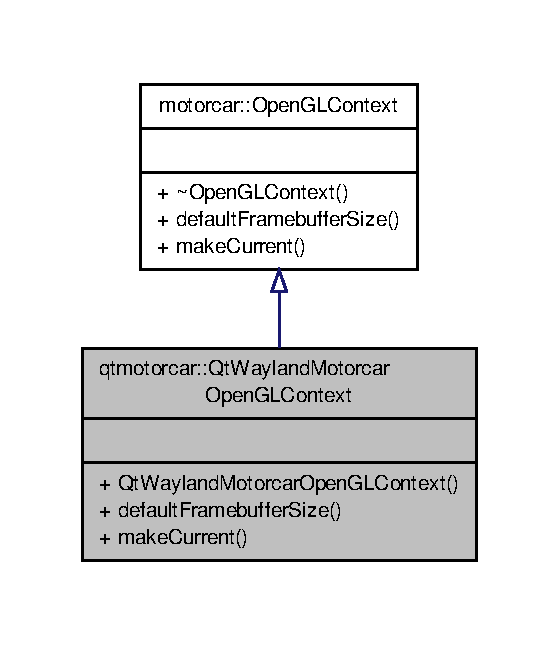
\includegraphics[width=268pt]{classqtmotorcar_1_1QtWaylandMotorcarOpenGLContext__inherit__graph}
\end{center}
\end{figure}


Collaboration diagram for qtmotorcar\-:\-:Qt\-Wayland\-Motorcar\-Open\-G\-L\-Context\-:
\nopagebreak
\begin{figure}[H]
\begin{center}
\leavevmode
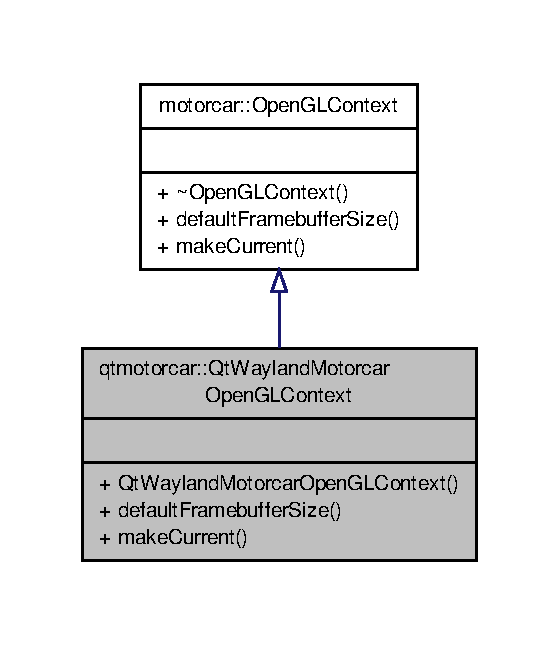
\includegraphics[width=268pt]{classqtmotorcar_1_1QtWaylandMotorcarOpenGLContext__coll__graph}
\end{center}
\end{figure}
\subsection*{Public Member Functions}
\begin{DoxyCompactItemize}
\item 
\hyperlink{classqtmotorcar_1_1QtWaylandMotorcarOpenGLContext_a18441ac9b0796170b33fdfb8c1154e30}{Qt\-Wayland\-Motorcar\-Open\-G\-L\-Context} (\hyperlink{classQOpenGLWindow}{Q\-Open\-G\-L\-Window} $\ast$window)
\item 
glm\-::ivec2 \hyperlink{classqtmotorcar_1_1QtWaylandMotorcarOpenGLContext_ab2a51af3b29de69f0a2d3d60d3bdbe82}{default\-Framebuffer\-Size} () override
\item 
void \hyperlink{classqtmotorcar_1_1QtWaylandMotorcarOpenGLContext_ae5f00ad8258f7c03466ad114b64e250a}{make\-Current} () override
\end{DoxyCompactItemize}


\subsection{Constructor \& Destructor Documentation}
\hypertarget{classqtmotorcar_1_1QtWaylandMotorcarOpenGLContext_a18441ac9b0796170b33fdfb8c1154e30}{\index{qtmotorcar\-::\-Qt\-Wayland\-Motorcar\-Open\-G\-L\-Context@{qtmotorcar\-::\-Qt\-Wayland\-Motorcar\-Open\-G\-L\-Context}!Qt\-Wayland\-Motorcar\-Open\-G\-L\-Context@{Qt\-Wayland\-Motorcar\-Open\-G\-L\-Context}}
\index{Qt\-Wayland\-Motorcar\-Open\-G\-L\-Context@{Qt\-Wayland\-Motorcar\-Open\-G\-L\-Context}!qtmotorcar::QtWaylandMotorcarOpenGLContext@{qtmotorcar\-::\-Qt\-Wayland\-Motorcar\-Open\-G\-L\-Context}}
\subsubsection[{Qt\-Wayland\-Motorcar\-Open\-G\-L\-Context}]{\setlength{\rightskip}{0pt plus 5cm}qtmotorcar\-::\-Qt\-Wayland\-Motorcar\-Open\-G\-L\-Context\-::\-Qt\-Wayland\-Motorcar\-Open\-G\-L\-Context (
\begin{DoxyParamCaption}
\item[{{\bf Q\-Open\-G\-L\-Window} $\ast$}]{window}
\end{DoxyParamCaption}
)}}\label{classqtmotorcar_1_1QtWaylandMotorcarOpenGLContext_a18441ac9b0796170b33fdfb8c1154e30}


\subsection{Member Function Documentation}
\hypertarget{classqtmotorcar_1_1QtWaylandMotorcarOpenGLContext_ab2a51af3b29de69f0a2d3d60d3bdbe82}{\index{qtmotorcar\-::\-Qt\-Wayland\-Motorcar\-Open\-G\-L\-Context@{qtmotorcar\-::\-Qt\-Wayland\-Motorcar\-Open\-G\-L\-Context}!default\-Framebuffer\-Size@{default\-Framebuffer\-Size}}
\index{default\-Framebuffer\-Size@{default\-Framebuffer\-Size}!qtmotorcar::QtWaylandMotorcarOpenGLContext@{qtmotorcar\-::\-Qt\-Wayland\-Motorcar\-Open\-G\-L\-Context}}
\subsubsection[{default\-Framebuffer\-Size}]{\setlength{\rightskip}{0pt plus 5cm}glm\-::ivec2 qtmotorcar\-::\-Qt\-Wayland\-Motorcar\-Open\-G\-L\-Context\-::default\-Framebuffer\-Size (
\begin{DoxyParamCaption}
{}
\end{DoxyParamCaption}
)\hspace{0.3cm}{\ttfamily [override]}, {\ttfamily [virtual]}}}\label{classqtmotorcar_1_1QtWaylandMotorcarOpenGLContext_ab2a51af3b29de69f0a2d3d60d3bdbe82}


Implements \hyperlink{classmotorcar_1_1OpenGLContext_a4a60274f217b9d71ff54ad60351b4127}{motorcar\-::\-Open\-G\-L\-Context}.

\hypertarget{classqtmotorcar_1_1QtWaylandMotorcarOpenGLContext_ae5f00ad8258f7c03466ad114b64e250a}{\index{qtmotorcar\-::\-Qt\-Wayland\-Motorcar\-Open\-G\-L\-Context@{qtmotorcar\-::\-Qt\-Wayland\-Motorcar\-Open\-G\-L\-Context}!make\-Current@{make\-Current}}
\index{make\-Current@{make\-Current}!qtmotorcar::QtWaylandMotorcarOpenGLContext@{qtmotorcar\-::\-Qt\-Wayland\-Motorcar\-Open\-G\-L\-Context}}
\subsubsection[{make\-Current}]{\setlength{\rightskip}{0pt plus 5cm}void qtmotorcar\-::\-Qt\-Wayland\-Motorcar\-Open\-G\-L\-Context\-::make\-Current (
\begin{DoxyParamCaption}
{}
\end{DoxyParamCaption}
)\hspace{0.3cm}{\ttfamily [override]}, {\ttfamily [virtual]}}}\label{classqtmotorcar_1_1QtWaylandMotorcarOpenGLContext_ae5f00ad8258f7c03466ad114b64e250a}


Implements \hyperlink{classmotorcar_1_1OpenGLContext_ae8b9c712092d01b69766469ab196ab80}{motorcar\-::\-Open\-G\-L\-Context}.



The documentation for this class was generated from the following files\-:\begin{DoxyCompactItemize}
\item 
/home/dave/thesis/qtwayland-\/motorcar-\/compositor/qt/src/\hyperlink{qtwaylandmotorcaropenglcontext_8h}{qtwaylandmotorcaropenglcontext.\-h}\item 
/home/dave/thesis/qtwayland-\/motorcar-\/compositor/qt/src/\hyperlink{qtwaylandmotorcaropenglcontext_8cpp}{qtwaylandmotorcaropenglcontext.\-cpp}\end{DoxyCompactItemize}

\hypertarget{classqtmotorcar_1_1QtWaylandMotorcarSurface}{\section{qtmotorcar\-:\-:Qt\-Wayland\-Motorcar\-Surface Class Reference}
\label{classqtmotorcar_1_1QtWaylandMotorcarSurface}\index{qtmotorcar\-::\-Qt\-Wayland\-Motorcar\-Surface@{qtmotorcar\-::\-Qt\-Wayland\-Motorcar\-Surface}}
}


{\ttfamily \#include $<$qtwaylandmotorcarsurface.\-h$>$}



Inheritance diagram for qtmotorcar\-:\-:Qt\-Wayland\-Motorcar\-Surface\-:
\nopagebreak
\begin{figure}[H]
\begin{center}
\leavevmode
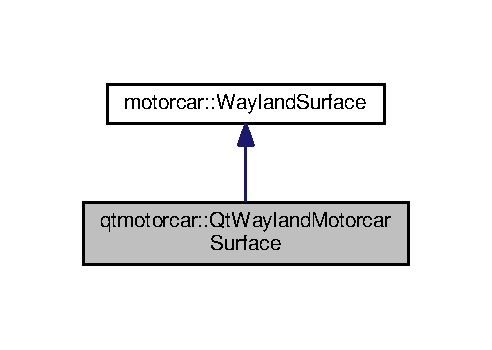
\includegraphics[width=236pt]{classqtmotorcar_1_1QtWaylandMotorcarSurface__inherit__graph}
\end{center}
\end{figure}


Collaboration diagram for qtmotorcar\-:\-:Qt\-Wayland\-Motorcar\-Surface\-:
\nopagebreak
\begin{figure}[H]
\begin{center}
\leavevmode
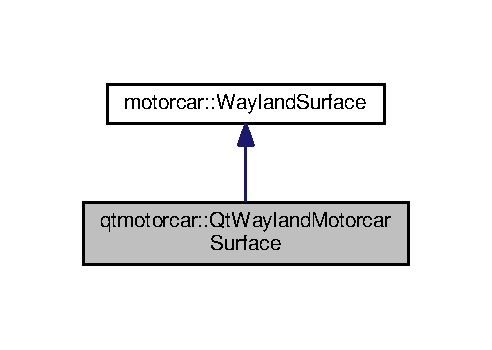
\includegraphics[width=236pt]{classqtmotorcar_1_1QtWaylandMotorcarSurface__coll__graph}
\end{center}
\end{figure}
\subsection*{Public Member Functions}
\begin{DoxyCompactItemize}
\item 
\hyperlink{classqtmotorcar_1_1QtWaylandMotorcarSurface_a054d4981e7da338c72e4fa6572869b60}{Qt\-Wayland\-Motorcar\-Surface} (Q\-Wayland\-Surface $\ast$\hyperlink{simple-egl_8cpp_a0720952aa1caded45b5bcdce589663a9}{surface}, \hyperlink{classqtmotorcar_1_1QtWaylandMotorcarCompositor}{Qt\-Wayland\-Motorcar\-Compositor} $\ast$compositor, \hyperlink{classmotorcar_1_1WaylandSurface_a7715a41b6776800656722407ec01e0a5}{motorcar\-::\-Wayland\-Surface\-::\-Surface\-Type} \hyperlink{classmotorcar_1_1WaylandSurface_a0e6e5e2455666f607a8ddb2479ba8e88}{type})
\item 
\hyperlink{classqtmotorcar_1_1QtWaylandMotorcarSurface_a0d9d57d75c14c209484174e47308f72f}{$\sim$\-Qt\-Wayland\-Motorcar\-Surface} ()
\item 
G\-Luint \hyperlink{classqtmotorcar_1_1QtWaylandMotorcarSurface_a573c52cdacb8f16c06ecd111bddabef6}{texture} () override
\begin{DoxyCompactList}\small\item\em Get the texture handle for this surface. \end{DoxyCompactList}\item 
glm\-::ivec2 \hyperlink{classqtmotorcar_1_1QtWaylandMotorcarSurface_ad5e6f75c146a2952652deaf866ee22a7}{size} () override
\begin{DoxyCompactList}\small\item\em Get the size of this surface in surface local coordinates. \end{DoxyCompactList}\item 
void \hyperlink{classqtmotorcar_1_1QtWaylandMotorcarSurface_abb0d9d5b6a226ab201fc1c0065d1843a}{set\-Size} (glm\-::ivec2 new\-Size) override
\begin{DoxyCompactList}\small\item\em Set the size of this surface in surface local coordinates. \end{DoxyCompactList}\item 
glm\-::ivec2 \hyperlink{classqtmotorcar_1_1QtWaylandMotorcarSurface_ad405b91565405e6a08d86ac5d59f3f08}{position} () override
\begin{DoxyCompactList}\small\item\em Get the position of this surface in parent surface-\/local coordinates. \end{DoxyCompactList}\item 
\hyperlink{classmotorcar_1_1WaylandSurface_a12a62c259b5041c6780c703ec2f12f01}{Wayland\-Surface} $\ast$ \hyperlink{classqtmotorcar_1_1QtWaylandMotorcarSurface_a3b0aed06d7ed9287497bc342f9fc787b}{parent\-Surface} () override
\begin{DoxyCompactList}\small\item\em return the parent surface \end{DoxyCompactList}\item 
void \hyperlink{classqtmotorcar_1_1QtWaylandMotorcarSurface_ae898706dcf80a2f00ed2477c570dcebe}{prepare} () override
\begin{DoxyCompactList}\small\item\em do any per-\/frame setup required for drawing \end{DoxyCompactList}\item 
void \hyperlink{classqtmotorcar_1_1QtWaylandMotorcarSurface_a7deebcf58954f82c8d5741af054414a7}{send\-Event} (const \hyperlink{classmotorcar_1_1Event}{motorcar\-::\-Event} \&event) override
\item 
bool \hyperlink{classqtmotorcar_1_1QtWaylandMotorcarSurface_a3bea85a2a6a3079e60c3b37dd08aebc6}{valid} () override
\begin{DoxyCompactList}\small\item\em returns whether or not the surface is ready to draw \end{DoxyCompactList}\item 
Q\-Wayland\-Surface $\ast$ \hyperlink{classqtmotorcar_1_1QtWaylandMotorcarSurface_aeac2b36246941755d0bedaf1c9fe773b}{surface} () const 
\item 
void \hyperlink{classqtmotorcar_1_1QtWaylandMotorcarSurface_aa7921de176d4d39fe076f145dd382e75}{set\-Surface} (Q\-Wayland\-Surface $\ast$\hyperlink{simple-egl_8cpp_a0720952aa1caded45b5bcdce589663a9}{surface})
\end{DoxyCompactItemize}
\subsection*{Additional Inherited Members}


\subsection{Constructor \& Destructor Documentation}
\hypertarget{classqtmotorcar_1_1QtWaylandMotorcarSurface_a054d4981e7da338c72e4fa6572869b60}{\index{qtmotorcar\-::\-Qt\-Wayland\-Motorcar\-Surface@{qtmotorcar\-::\-Qt\-Wayland\-Motorcar\-Surface}!Qt\-Wayland\-Motorcar\-Surface@{Qt\-Wayland\-Motorcar\-Surface}}
\index{Qt\-Wayland\-Motorcar\-Surface@{Qt\-Wayland\-Motorcar\-Surface}!qtmotorcar::QtWaylandMotorcarSurface@{qtmotorcar\-::\-Qt\-Wayland\-Motorcar\-Surface}}
\subsubsection[{Qt\-Wayland\-Motorcar\-Surface}]{\setlength{\rightskip}{0pt plus 5cm}Qt\-Wayland\-Motorcar\-Surface\-::\-Qt\-Wayland\-Motorcar\-Surface (
\begin{DoxyParamCaption}
\item[{Q\-Wayland\-Surface $\ast$}]{surface, }
\item[{{\bf Qt\-Wayland\-Motorcar\-Compositor} $\ast$}]{compositor, }
\item[{{\bf motorcar\-::\-Wayland\-Surface\-::\-Surface\-Type}}]{type}
\end{DoxyParamCaption}
)}}\label{classqtmotorcar_1_1QtWaylandMotorcarSurface_a054d4981e7da338c72e4fa6572869b60}
\hypertarget{classqtmotorcar_1_1QtWaylandMotorcarSurface_a0d9d57d75c14c209484174e47308f72f}{\index{qtmotorcar\-::\-Qt\-Wayland\-Motorcar\-Surface@{qtmotorcar\-::\-Qt\-Wayland\-Motorcar\-Surface}!$\sim$\-Qt\-Wayland\-Motorcar\-Surface@{$\sim$\-Qt\-Wayland\-Motorcar\-Surface}}
\index{$\sim$\-Qt\-Wayland\-Motorcar\-Surface@{$\sim$\-Qt\-Wayland\-Motorcar\-Surface}!qtmotorcar::QtWaylandMotorcarSurface@{qtmotorcar\-::\-Qt\-Wayland\-Motorcar\-Surface}}
\subsubsection[{$\sim$\-Qt\-Wayland\-Motorcar\-Surface}]{\setlength{\rightskip}{0pt plus 5cm}qtmotorcar\-::\-Qt\-Wayland\-Motorcar\-Surface\-::$\sim$\-Qt\-Wayland\-Motorcar\-Surface (
\begin{DoxyParamCaption}
{}
\end{DoxyParamCaption}
)\hspace{0.3cm}{\ttfamily [inline]}}}\label{classqtmotorcar_1_1QtWaylandMotorcarSurface_a0d9d57d75c14c209484174e47308f72f}


\subsection{Member Function Documentation}
\hypertarget{classqtmotorcar_1_1QtWaylandMotorcarSurface_a3b0aed06d7ed9287497bc342f9fc787b}{\index{qtmotorcar\-::\-Qt\-Wayland\-Motorcar\-Surface@{qtmotorcar\-::\-Qt\-Wayland\-Motorcar\-Surface}!parent\-Surface@{parent\-Surface}}
\index{parent\-Surface@{parent\-Surface}!qtmotorcar::QtWaylandMotorcarSurface@{qtmotorcar\-::\-Qt\-Wayland\-Motorcar\-Surface}}
\subsubsection[{parent\-Surface}]{\setlength{\rightskip}{0pt plus 5cm}{\bf motorcar\-::\-Wayland\-Surface} $\ast$ Qt\-Wayland\-Motorcar\-Surface\-::parent\-Surface (
\begin{DoxyParamCaption}
{}
\end{DoxyParamCaption}
)\hspace{0.3cm}{\ttfamily [override]}, {\ttfamily [virtual]}}}\label{classqtmotorcar_1_1QtWaylandMotorcarSurface_a3b0aed06d7ed9287497bc342f9fc787b}


return the parent surface 



Implements \hyperlink{classmotorcar_1_1WaylandSurface_a94b48df54c92d9046f786d4d7f5d4ff2}{motorcar\-::\-Wayland\-Surface}.

\hypertarget{classqtmotorcar_1_1QtWaylandMotorcarSurface_ad405b91565405e6a08d86ac5d59f3f08}{\index{qtmotorcar\-::\-Qt\-Wayland\-Motorcar\-Surface@{qtmotorcar\-::\-Qt\-Wayland\-Motorcar\-Surface}!position@{position}}
\index{position@{position}!qtmotorcar::QtWaylandMotorcarSurface@{qtmotorcar\-::\-Qt\-Wayland\-Motorcar\-Surface}}
\subsubsection[{position}]{\setlength{\rightskip}{0pt plus 5cm}glm\-::ivec2 Qt\-Wayland\-Motorcar\-Surface\-::position (
\begin{DoxyParamCaption}
{}
\end{DoxyParamCaption}
)\hspace{0.3cm}{\ttfamily [override]}, {\ttfamily [virtual]}}}\label{classqtmotorcar_1_1QtWaylandMotorcarSurface_ad405b91565405e6a08d86ac5d59f3f08}


Get the position of this surface in parent surface-\/local coordinates. 



Implements \hyperlink{classmotorcar_1_1WaylandSurface_a22f62be59ac9b8b76a2b2f467f0b1277}{motorcar\-::\-Wayland\-Surface}.

\hypertarget{classqtmotorcar_1_1QtWaylandMotorcarSurface_ae898706dcf80a2f00ed2477c570dcebe}{\index{qtmotorcar\-::\-Qt\-Wayland\-Motorcar\-Surface@{qtmotorcar\-::\-Qt\-Wayland\-Motorcar\-Surface}!prepare@{prepare}}
\index{prepare@{prepare}!qtmotorcar::QtWaylandMotorcarSurface@{qtmotorcar\-::\-Qt\-Wayland\-Motorcar\-Surface}}
\subsubsection[{prepare}]{\setlength{\rightskip}{0pt plus 5cm}void Qt\-Wayland\-Motorcar\-Surface\-::prepare (
\begin{DoxyParamCaption}
{}
\end{DoxyParamCaption}
)\hspace{0.3cm}{\ttfamily [override]}, {\ttfamily [virtual]}}}\label{classqtmotorcar_1_1QtWaylandMotorcarSurface_ae898706dcf80a2f00ed2477c570dcebe}


do any per-\/frame setup required for drawing 



Implements \hyperlink{classmotorcar_1_1WaylandSurface_a63669771c03ce580fec8a0099dbd294e}{motorcar\-::\-Wayland\-Surface}.

\hypertarget{classqtmotorcar_1_1QtWaylandMotorcarSurface_a7deebcf58954f82c8d5741af054414a7}{\index{qtmotorcar\-::\-Qt\-Wayland\-Motorcar\-Surface@{qtmotorcar\-::\-Qt\-Wayland\-Motorcar\-Surface}!send\-Event@{send\-Event}}
\index{send\-Event@{send\-Event}!qtmotorcar::QtWaylandMotorcarSurface@{qtmotorcar\-::\-Qt\-Wayland\-Motorcar\-Surface}}
\subsubsection[{send\-Event}]{\setlength{\rightskip}{0pt plus 5cm}void Qt\-Wayland\-Motorcar\-Surface\-::send\-Event (
\begin{DoxyParamCaption}
\item[{const {\bf motorcar\-::\-Event} \&}]{event}
\end{DoxyParamCaption}
)\hspace{0.3cm}{\ttfamily [override]}, {\ttfamily [virtual]}}}\label{classqtmotorcar_1_1QtWaylandMotorcarSurface_a7deebcf58954f82c8d5741af054414a7}


Implements \hyperlink{classmotorcar_1_1WaylandSurface_a8d709e7d02ee7f7b8b3343590e518993}{motorcar\-::\-Wayland\-Surface}.

\hypertarget{classqtmotorcar_1_1QtWaylandMotorcarSurface_abb0d9d5b6a226ab201fc1c0065d1843a}{\index{qtmotorcar\-::\-Qt\-Wayland\-Motorcar\-Surface@{qtmotorcar\-::\-Qt\-Wayland\-Motorcar\-Surface}!set\-Size@{set\-Size}}
\index{set\-Size@{set\-Size}!qtmotorcar::QtWaylandMotorcarSurface@{qtmotorcar\-::\-Qt\-Wayland\-Motorcar\-Surface}}
\subsubsection[{set\-Size}]{\setlength{\rightskip}{0pt plus 5cm}void Qt\-Wayland\-Motorcar\-Surface\-::set\-Size (
\begin{DoxyParamCaption}
\item[{glm\-::ivec2}]{new\-Size}
\end{DoxyParamCaption}
)\hspace{0.3cm}{\ttfamily [override]}, {\ttfamily [virtual]}}}\label{classqtmotorcar_1_1QtWaylandMotorcarSurface_abb0d9d5b6a226ab201fc1c0065d1843a}


Set the size of this surface in surface local coordinates. 



Implements \hyperlink{classmotorcar_1_1WaylandSurface_a7d2ee4e48305c5510916ba9bdcb46a44}{motorcar\-::\-Wayland\-Surface}.

\hypertarget{classqtmotorcar_1_1QtWaylandMotorcarSurface_aa7921de176d4d39fe076f145dd382e75}{\index{qtmotorcar\-::\-Qt\-Wayland\-Motorcar\-Surface@{qtmotorcar\-::\-Qt\-Wayland\-Motorcar\-Surface}!set\-Surface@{set\-Surface}}
\index{set\-Surface@{set\-Surface}!qtmotorcar::QtWaylandMotorcarSurface@{qtmotorcar\-::\-Qt\-Wayland\-Motorcar\-Surface}}
\subsubsection[{set\-Surface}]{\setlength{\rightskip}{0pt plus 5cm}void Qt\-Wayland\-Motorcar\-Surface\-::set\-Surface (
\begin{DoxyParamCaption}
\item[{Q\-Wayland\-Surface $\ast$}]{surface}
\end{DoxyParamCaption}
)}}\label{classqtmotorcar_1_1QtWaylandMotorcarSurface_aa7921de176d4d39fe076f145dd382e75}
\hypertarget{classqtmotorcar_1_1QtWaylandMotorcarSurface_ad5e6f75c146a2952652deaf866ee22a7}{\index{qtmotorcar\-::\-Qt\-Wayland\-Motorcar\-Surface@{qtmotorcar\-::\-Qt\-Wayland\-Motorcar\-Surface}!size@{size}}
\index{size@{size}!qtmotorcar::QtWaylandMotorcarSurface@{qtmotorcar\-::\-Qt\-Wayland\-Motorcar\-Surface}}
\subsubsection[{size}]{\setlength{\rightskip}{0pt plus 5cm}glm\-::ivec2 Qt\-Wayland\-Motorcar\-Surface\-::size (
\begin{DoxyParamCaption}
{}
\end{DoxyParamCaption}
)\hspace{0.3cm}{\ttfamily [override]}, {\ttfamily [virtual]}}}\label{classqtmotorcar_1_1QtWaylandMotorcarSurface_ad5e6f75c146a2952652deaf866ee22a7}


Get the size of this surface in surface local coordinates. 



Implements \hyperlink{classmotorcar_1_1WaylandSurface_a06182d612aaf0d07780e498066aaca1b}{motorcar\-::\-Wayland\-Surface}.

\hypertarget{classqtmotorcar_1_1QtWaylandMotorcarSurface_aeac2b36246941755d0bedaf1c9fe773b}{\index{qtmotorcar\-::\-Qt\-Wayland\-Motorcar\-Surface@{qtmotorcar\-::\-Qt\-Wayland\-Motorcar\-Surface}!surface@{surface}}
\index{surface@{surface}!qtmotorcar::QtWaylandMotorcarSurface@{qtmotorcar\-::\-Qt\-Wayland\-Motorcar\-Surface}}
\subsubsection[{surface}]{\setlength{\rightskip}{0pt plus 5cm}Q\-Wayland\-Surface $\ast$ Qt\-Wayland\-Motorcar\-Surface\-::surface (
\begin{DoxyParamCaption}
{}
\end{DoxyParamCaption}
) const}}\label{classqtmotorcar_1_1QtWaylandMotorcarSurface_aeac2b36246941755d0bedaf1c9fe773b}
\hypertarget{classqtmotorcar_1_1QtWaylandMotorcarSurface_a573c52cdacb8f16c06ecd111bddabef6}{\index{qtmotorcar\-::\-Qt\-Wayland\-Motorcar\-Surface@{qtmotorcar\-::\-Qt\-Wayland\-Motorcar\-Surface}!texture@{texture}}
\index{texture@{texture}!qtmotorcar::QtWaylandMotorcarSurface@{qtmotorcar\-::\-Qt\-Wayland\-Motorcar\-Surface}}
\subsubsection[{texture}]{\setlength{\rightskip}{0pt plus 5cm}G\-Luint Qt\-Wayland\-Motorcar\-Surface\-::texture (
\begin{DoxyParamCaption}
{}
\end{DoxyParamCaption}
)\hspace{0.3cm}{\ttfamily [override]}, {\ttfamily [virtual]}}}\label{classqtmotorcar_1_1QtWaylandMotorcarSurface_a573c52cdacb8f16c06ecd111bddabef6}


Get the texture handle for this surface. 



Implements \hyperlink{classmotorcar_1_1WaylandSurface_aa8ae13d97dae8dfbb610ca6f4ab2b745}{motorcar\-::\-Wayland\-Surface}.

\hypertarget{classqtmotorcar_1_1QtWaylandMotorcarSurface_a3bea85a2a6a3079e60c3b37dd08aebc6}{\index{qtmotorcar\-::\-Qt\-Wayland\-Motorcar\-Surface@{qtmotorcar\-::\-Qt\-Wayland\-Motorcar\-Surface}!valid@{valid}}
\index{valid@{valid}!qtmotorcar::QtWaylandMotorcarSurface@{qtmotorcar\-::\-Qt\-Wayland\-Motorcar\-Surface}}
\subsubsection[{valid}]{\setlength{\rightskip}{0pt plus 5cm}bool Qt\-Wayland\-Motorcar\-Surface\-::valid (
\begin{DoxyParamCaption}
{}
\end{DoxyParamCaption}
)\hspace{0.3cm}{\ttfamily [override]}, {\ttfamily [virtual]}}}\label{classqtmotorcar_1_1QtWaylandMotorcarSurface_a3bea85a2a6a3079e60c3b37dd08aebc6}


returns whether or not the surface is ready to draw 



Implements \hyperlink{classmotorcar_1_1WaylandSurface_af2f54076ec690f4d478771183c9b0db5}{motorcar\-::\-Wayland\-Surface}.



The documentation for this class was generated from the following files\-:\begin{DoxyCompactItemize}
\item 
/home/dave/thesis/motorcar/src/compositor/qt/\hyperlink{qtwaylandmotorcarsurface_8h}{qtwaylandmotorcarsurface.\-h}\item 
/home/dave/thesis/motorcar/src/compositor/qt/\hyperlink{qtwaylandmotorcarsurface_8cpp}{qtwaylandmotorcarsurface.\-cpp}\end{DoxyCompactItemize}

\hypertarget{classQtwaylandSurfaceNode}{\section{Qtwayland\-Surface\-Node Class Reference}
\label{classQtwaylandSurfaceNode}\index{Qtwayland\-Surface\-Node@{Qtwayland\-Surface\-Node}}
}


{\ttfamily \#include $<$qtwaylandsurfacenode.\-h$>$}



Collaboration diagram for Qtwayland\-Surface\-Node\-:
\nopagebreak
\begin{figure}[H]
\begin{center}
\leavevmode
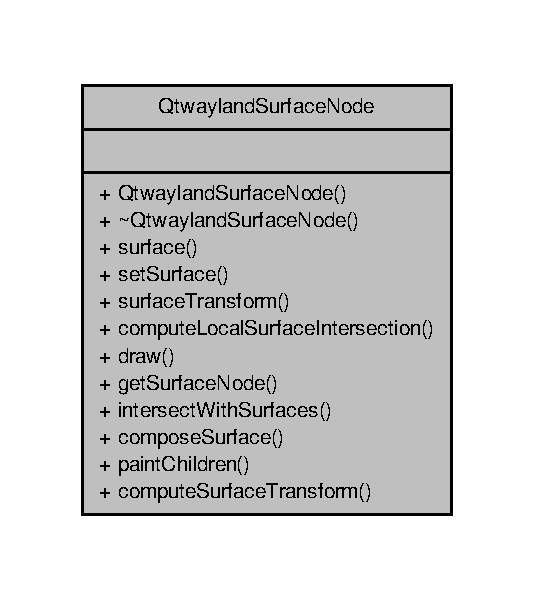
\includegraphics[width=256pt]{classQtwaylandSurfaceNode__coll__graph}
\end{center}
\end{figure}
\subsection*{Public Member Functions}
\begin{DoxyCompactItemize}
\item 
\hyperlink{classQtwaylandSurfaceNode_a582fc9fb7bee6fecc1935c229bc84e72}{Qtwayland\-Surface\-Node} (Q\-Object $\ast$parent, Q\-Wayland\-Surface $\ast$\hyperlink{classQtwaylandSurfaceNode_a8f07c78202a2faa244d9d6c389c03951}{surface}, glm\-::mat4 transform=glm\-::mat4(1))
\item 
virtual \hyperlink{classQtwaylandSurfaceNode_af762332b319b9239e955d4a69b165c14}{$\sim$\-Qtwayland\-Surface\-Node} ()
\item 
Q\-Wayland\-Surface $\ast$ \hyperlink{classQtwaylandSurfaceNode_a8f07c78202a2faa244d9d6c389c03951}{surface} () const 
\item 
void \hyperlink{classQtwaylandSurfaceNode_ace08a2691d01fe10087e9b6997d1523b}{set\-Surface} (Q\-Wayland\-Surface $\ast$\hyperlink{classQtwaylandSurfaceNode_a8f07c78202a2faa244d9d6c389c03951}{surface})
\item 
glm\-::mat4 \hyperlink{classQtwaylandSurfaceNode_a8f88e9c392012d312206da67d6ea81ed}{surface\-Transform} () const 
\item 
bool \hyperlink{classQtwaylandSurfaceNode_a0307e078cfa9bcd6aaad60830ab5b3a6}{compute\-Local\-Surface\-Intersection} (const Geometry\-::\-Ray \&local\-Ray, Q\-Point\-F \&local\-Intersection, float \&t) const 
\item 
virtual bool \hyperlink{classQtwaylandSurfaceNode_a620c58196d857fe5146cfff49c6787fd}{draw} (Display\-Node $\ast$display)
\item 
virtual \hyperlink{classQtwaylandSurfaceNode}{Qtwayland\-Surface\-Node} $\ast$ \hyperlink{classQtwaylandSurfaceNode_a72db2bcd85e26d7f0332175f691a0dfd}{get\-Surface\-Node} (const Q\-Wayland\-Surface $\ast$\hyperlink{classQtwaylandSurfaceNode_a8f07c78202a2faa244d9d6c389c03951}{surface}=N\-U\-L\-L)
\item 
virtual \\*
Scene\-Graph\-Node\-::\-Ray\-Surface\-Intersection $\ast$ \hyperlink{classQtwaylandSurfaceNode_a82a9f9f93675df011cfd350a1857ea8b}{intersect\-With\-Surfaces} (const Geometry\-::\-Ray \&ray)
\item 
G\-Luint \hyperlink{classQtwaylandSurfaceNode_a16ad301303ca42fa9a2ad3d1799cf1a2}{compose\-Surface} (Q\-Wayland\-Surface $\ast$\hyperlink{classQtwaylandSurfaceNode_a8f07c78202a2faa244d9d6c389c03951}{surface}, \hyperlink{classOpenGLData}{Open\-G\-L\-Data} $\ast$gl\-Data)
\item 
void \hyperlink{classQtwaylandSurfaceNode_a0de0e4cbe5312d91334e091160ac4bce}{paint\-Children} (Q\-Wayland\-Surface $\ast$\hyperlink{classQtwaylandSurfaceNode_a8f07c78202a2faa244d9d6c389c03951}{surface}, Q\-Wayland\-Surface $\ast$window, \hyperlink{classOpenGLData}{Open\-G\-L\-Data} $\ast$gl\-Data)
\item 
void \hyperlink{classQtwaylandSurfaceNode_a9917572c6241c4a7593b4c9cd9f8c290}{compute\-Surface\-Transform} (float ppcm)
\end{DoxyCompactItemize}


\subsection{Constructor \& Destructor Documentation}
\hypertarget{classQtwaylandSurfaceNode_a582fc9fb7bee6fecc1935c229bc84e72}{\index{Qtwayland\-Surface\-Node@{Qtwayland\-Surface\-Node}!Qtwayland\-Surface\-Node@{Qtwayland\-Surface\-Node}}
\index{Qtwayland\-Surface\-Node@{Qtwayland\-Surface\-Node}!QtwaylandSurfaceNode@{Qtwayland\-Surface\-Node}}
\subsubsection[{Qtwayland\-Surface\-Node}]{\setlength{\rightskip}{0pt plus 5cm}Qtwayland\-Surface\-Node\-::\-Qtwayland\-Surface\-Node (
\begin{DoxyParamCaption}
\item[{Q\-Object $\ast$}]{parent, }
\item[{Q\-Wayland\-Surface $\ast$}]{surface, }
\item[{glm\-::mat4}]{transform = {\ttfamily glm\-:\-:mat4(1)}}
\end{DoxyParamCaption}
)}}\label{classQtwaylandSurfaceNode_a582fc9fb7bee6fecc1935c229bc84e72}
\hypertarget{classQtwaylandSurfaceNode_af762332b319b9239e955d4a69b165c14}{\index{Qtwayland\-Surface\-Node@{Qtwayland\-Surface\-Node}!$\sim$\-Qtwayland\-Surface\-Node@{$\sim$\-Qtwayland\-Surface\-Node}}
\index{$\sim$\-Qtwayland\-Surface\-Node@{$\sim$\-Qtwayland\-Surface\-Node}!QtwaylandSurfaceNode@{Qtwayland\-Surface\-Node}}
\subsubsection[{$\sim$\-Qtwayland\-Surface\-Node}]{\setlength{\rightskip}{0pt plus 5cm}Qtwayland\-Surface\-Node\-::$\sim$\-Qtwayland\-Surface\-Node (
\begin{DoxyParamCaption}
{}
\end{DoxyParamCaption}
)\hspace{0.3cm}{\ttfamily [virtual]}}}\label{classQtwaylandSurfaceNode_af762332b319b9239e955d4a69b165c14}


\subsection{Member Function Documentation}
\hypertarget{classQtwaylandSurfaceNode_a16ad301303ca42fa9a2ad3d1799cf1a2}{\index{Qtwayland\-Surface\-Node@{Qtwayland\-Surface\-Node}!compose\-Surface@{compose\-Surface}}
\index{compose\-Surface@{compose\-Surface}!QtwaylandSurfaceNode@{Qtwayland\-Surface\-Node}}
\subsubsection[{compose\-Surface}]{\setlength{\rightskip}{0pt plus 5cm}G\-Luint Qtwayland\-Surface\-Node\-::compose\-Surface (
\begin{DoxyParamCaption}
\item[{Q\-Wayland\-Surface $\ast$}]{surface, }
\item[{{\bf Open\-G\-L\-Data} $\ast$}]{gl\-Data}
\end{DoxyParamCaption}
)}}\label{classQtwaylandSurfaceNode_a16ad301303ca42fa9a2ad3d1799cf1a2}
\hypertarget{classQtwaylandSurfaceNode_a0307e078cfa9bcd6aaad60830ab5b3a6}{\index{Qtwayland\-Surface\-Node@{Qtwayland\-Surface\-Node}!compute\-Local\-Surface\-Intersection@{compute\-Local\-Surface\-Intersection}}
\index{compute\-Local\-Surface\-Intersection@{compute\-Local\-Surface\-Intersection}!QtwaylandSurfaceNode@{Qtwayland\-Surface\-Node}}
\subsubsection[{compute\-Local\-Surface\-Intersection}]{\setlength{\rightskip}{0pt plus 5cm}bool Qtwayland\-Surface\-Node\-::compute\-Local\-Surface\-Intersection (
\begin{DoxyParamCaption}
\item[{const Geometry\-::\-Ray \&}]{local\-Ray, }
\item[{Q\-Point\-F \&}]{local\-Intersection, }
\item[{float \&}]{t}
\end{DoxyParamCaption}
) const}}\label{classQtwaylandSurfaceNode_a0307e078cfa9bcd6aaad60830ab5b3a6}
\hypertarget{classQtwaylandSurfaceNode_a9917572c6241c4a7593b4c9cd9f8c290}{\index{Qtwayland\-Surface\-Node@{Qtwayland\-Surface\-Node}!compute\-Surface\-Transform@{compute\-Surface\-Transform}}
\index{compute\-Surface\-Transform@{compute\-Surface\-Transform}!QtwaylandSurfaceNode@{Qtwayland\-Surface\-Node}}
\subsubsection[{compute\-Surface\-Transform}]{\setlength{\rightskip}{0pt plus 5cm}void Qtwayland\-Surface\-Node\-::compute\-Surface\-Transform (
\begin{DoxyParamCaption}
\item[{float}]{ppcm}
\end{DoxyParamCaption}
)}}\label{classQtwaylandSurfaceNode_a9917572c6241c4a7593b4c9cd9f8c290}
\hypertarget{classQtwaylandSurfaceNode_a620c58196d857fe5146cfff49c6787fd}{\index{Qtwayland\-Surface\-Node@{Qtwayland\-Surface\-Node}!draw@{draw}}
\index{draw@{draw}!QtwaylandSurfaceNode@{Qtwayland\-Surface\-Node}}
\subsubsection[{draw}]{\setlength{\rightskip}{0pt plus 5cm}bool Qtwayland\-Surface\-Node\-::draw (
\begin{DoxyParamCaption}
\item[{Display\-Node $\ast$}]{display}
\end{DoxyParamCaption}
)\hspace{0.3cm}{\ttfamily [virtual]}}}\label{classQtwaylandSurfaceNode_a620c58196d857fe5146cfff49c6787fd}
\hypertarget{classQtwaylandSurfaceNode_a72db2bcd85e26d7f0332175f691a0dfd}{\index{Qtwayland\-Surface\-Node@{Qtwayland\-Surface\-Node}!get\-Surface\-Node@{get\-Surface\-Node}}
\index{get\-Surface\-Node@{get\-Surface\-Node}!QtwaylandSurfaceNode@{Qtwayland\-Surface\-Node}}
\subsubsection[{get\-Surface\-Node}]{\setlength{\rightskip}{0pt plus 5cm}{\bf Qtwayland\-Surface\-Node} $\ast$ Qtwayland\-Surface\-Node\-::get\-Surface\-Node (
\begin{DoxyParamCaption}
\item[{const Q\-Wayland\-Surface $\ast$}]{surface = {\ttfamily NULL}}
\end{DoxyParamCaption}
)\hspace{0.3cm}{\ttfamily [virtual]}}}\label{classQtwaylandSurfaceNode_a72db2bcd85e26d7f0332175f691a0dfd}
\hypertarget{classQtwaylandSurfaceNode_a82a9f9f93675df011cfd350a1857ea8b}{\index{Qtwayland\-Surface\-Node@{Qtwayland\-Surface\-Node}!intersect\-With\-Surfaces@{intersect\-With\-Surfaces}}
\index{intersect\-With\-Surfaces@{intersect\-With\-Surfaces}!QtwaylandSurfaceNode@{Qtwayland\-Surface\-Node}}
\subsubsection[{intersect\-With\-Surfaces}]{\setlength{\rightskip}{0pt plus 5cm}Scene\-Graph\-Node\-::\-Ray\-Surface\-Intersection $\ast$ Qtwayland\-Surface\-Node\-::intersect\-With\-Surfaces (
\begin{DoxyParamCaption}
\item[{const Geometry\-::\-Ray \&}]{ray}
\end{DoxyParamCaption}
)\hspace{0.3cm}{\ttfamily [virtual]}}}\label{classQtwaylandSurfaceNode_a82a9f9f93675df011cfd350a1857ea8b}
\hypertarget{classQtwaylandSurfaceNode_a0de0e4cbe5312d91334e091160ac4bce}{\index{Qtwayland\-Surface\-Node@{Qtwayland\-Surface\-Node}!paint\-Children@{paint\-Children}}
\index{paint\-Children@{paint\-Children}!QtwaylandSurfaceNode@{Qtwayland\-Surface\-Node}}
\subsubsection[{paint\-Children}]{\setlength{\rightskip}{0pt plus 5cm}void Qtwayland\-Surface\-Node\-::paint\-Children (
\begin{DoxyParamCaption}
\item[{Q\-Wayland\-Surface $\ast$}]{surface, }
\item[{Q\-Wayland\-Surface $\ast$}]{window, }
\item[{{\bf Open\-G\-L\-Data} $\ast$}]{gl\-Data}
\end{DoxyParamCaption}
)}}\label{classQtwaylandSurfaceNode_a0de0e4cbe5312d91334e091160ac4bce}
\hypertarget{classQtwaylandSurfaceNode_ace08a2691d01fe10087e9b6997d1523b}{\index{Qtwayland\-Surface\-Node@{Qtwayland\-Surface\-Node}!set\-Surface@{set\-Surface}}
\index{set\-Surface@{set\-Surface}!QtwaylandSurfaceNode@{Qtwayland\-Surface\-Node}}
\subsubsection[{set\-Surface}]{\setlength{\rightskip}{0pt plus 5cm}void Qtwayland\-Surface\-Node\-::set\-Surface (
\begin{DoxyParamCaption}
\item[{Q\-Wayland\-Surface $\ast$}]{surface}
\end{DoxyParamCaption}
)}}\label{classQtwaylandSurfaceNode_ace08a2691d01fe10087e9b6997d1523b}
\hypertarget{classQtwaylandSurfaceNode_a8f07c78202a2faa244d9d6c389c03951}{\index{Qtwayland\-Surface\-Node@{Qtwayland\-Surface\-Node}!surface@{surface}}
\index{surface@{surface}!QtwaylandSurfaceNode@{Qtwayland\-Surface\-Node}}
\subsubsection[{surface}]{\setlength{\rightskip}{0pt plus 5cm}Q\-Wayland\-Surface $\ast$ Qtwayland\-Surface\-Node\-::surface (
\begin{DoxyParamCaption}
{}
\end{DoxyParamCaption}
) const}}\label{classQtwaylandSurfaceNode_a8f07c78202a2faa244d9d6c389c03951}
\hypertarget{classQtwaylandSurfaceNode_a8f88e9c392012d312206da67d6ea81ed}{\index{Qtwayland\-Surface\-Node@{Qtwayland\-Surface\-Node}!surface\-Transform@{surface\-Transform}}
\index{surface\-Transform@{surface\-Transform}!QtwaylandSurfaceNode@{Qtwayland\-Surface\-Node}}
\subsubsection[{surface\-Transform}]{\setlength{\rightskip}{0pt plus 5cm}glm\-::mat4 Qtwayland\-Surface\-Node\-::surface\-Transform (
\begin{DoxyParamCaption}
{}
\end{DoxyParamCaption}
) const}}\label{classQtwaylandSurfaceNode_a8f88e9c392012d312206da67d6ea81ed}


The documentation for this class was generated from the following files\-:\begin{DoxyCompactItemize}
\item 
/home/dave/thesis/qtwayland-\/motorcar-\/compositor/qt/src/\hyperlink{qtwaylandsurfacenode_8h}{qtwaylandsurfacenode.\-h}\item 
/home/dave/thesis/qtwayland-\/motorcar-\/compositor/qt/src/\hyperlink{qtwaylandsurfacenode_8cpp}{qtwaylandsurfacenode.\-cpp}\end{DoxyCompactItemize}

\hypertarget{structmotorcar_1_1Geometry_1_1Ray}{\section{motorcar\-:\-:Geometry\-:\-:Ray Struct Reference}
\label{structmotorcar_1_1Geometry_1_1Ray}\index{motorcar\-::\-Geometry\-::\-Ray@{motorcar\-::\-Geometry\-::\-Ray}}
}


{\ttfamily \#include $<$geometry.\-h$>$}

\subsection*{Public Member Functions}
\begin{DoxyCompactItemize}
\item 
\hyperlink{structmotorcar_1_1Geometry_1_1Ray_a0e703633f6101262ee14d17831745ca4}{Ray} (glm\-::vec3 \hyperlink{structmotorcar_1_1Geometry_1_1Ray_ac58960f9f82f19c6f514ae6c948deb86}{p}, glm\-::vec3 \hyperlink{structmotorcar_1_1Geometry_1_1Ray_a7140db28237277781ecb792fc280a95d}{d})
\item 
\hyperlink{structmotorcar_1_1Geometry_1_1Ray}{Ray} \hyperlink{structmotorcar_1_1Geometry_1_1Ray_a7de7ddd9609a26bdd1f2fe74933dfff6}{transform} (glm\-::mat4 t) const 
\item 
glm\-::vec3 \hyperlink{structmotorcar_1_1Geometry_1_1Ray_af14d102bfe9fdf08bb3396ad33d928bd}{solve} (float t) const 
\item 
void \hyperlink{structmotorcar_1_1Geometry_1_1Ray_a058da6e22e8fdcd7e2aa301153c9fa16}{print} () const 
\item 
void \hyperlink{structmotorcar_1_1Geometry_1_1Ray_a7d9403aa28c33c40d4b7e3c64ce3776d}{draw} (\hyperlink{classmotorcar_1_1SceneGraphNode}{motorcar\-::\-Scene\-Graph\-Node} $\ast$parent, glm\-::vec3 color, glm\-::mat4 \hyperlink{structmotorcar_1_1Geometry_1_1Ray_a7de7ddd9609a26bdd1f2fe74933dfff6}{transform}=glm\-::mat4(1))
\end{DoxyCompactItemize}
\subsection*{Public Attributes}
\begin{DoxyCompactItemize}
\item 
glm\-::vec3 \hyperlink{structmotorcar_1_1Geometry_1_1Ray_ac58960f9f82f19c6f514ae6c948deb86}{p}
\item 
glm\-::vec3 \hyperlink{structmotorcar_1_1Geometry_1_1Ray_a7140db28237277781ecb792fc280a95d}{d}
\end{DoxyCompactItemize}


\subsection{Constructor \& Destructor Documentation}
\hypertarget{structmotorcar_1_1Geometry_1_1Ray_a0e703633f6101262ee14d17831745ca4}{\index{motorcar\-::\-Geometry\-::\-Ray@{motorcar\-::\-Geometry\-::\-Ray}!Ray@{Ray}}
\index{Ray@{Ray}!motorcar::Geometry::Ray@{motorcar\-::\-Geometry\-::\-Ray}}
\subsubsection[{Ray}]{\setlength{\rightskip}{0pt plus 5cm}Geometry\-::\-Ray\-::\-Ray (
\begin{DoxyParamCaption}
\item[{glm\-::vec3}]{p, }
\item[{glm\-::vec3}]{d}
\end{DoxyParamCaption}
)}}\label{structmotorcar_1_1Geometry_1_1Ray_a0e703633f6101262ee14d17831745ca4}


\subsection{Member Function Documentation}
\hypertarget{structmotorcar_1_1Geometry_1_1Ray_a7d9403aa28c33c40d4b7e3c64ce3776d}{\index{motorcar\-::\-Geometry\-::\-Ray@{motorcar\-::\-Geometry\-::\-Ray}!draw@{draw}}
\index{draw@{draw}!motorcar::Geometry::Ray@{motorcar\-::\-Geometry\-::\-Ray}}
\subsubsection[{draw}]{\setlength{\rightskip}{0pt plus 5cm}void Geometry\-::\-Ray\-::draw (
\begin{DoxyParamCaption}
\item[{{\bf motorcar\-::\-Scene\-Graph\-Node} $\ast$}]{parent, }
\item[{glm\-::vec3}]{color, }
\item[{glm\-::mat4}]{transform = {\ttfamily glm\-:\-:mat4(1)}}
\end{DoxyParamCaption}
)}}\label{structmotorcar_1_1Geometry_1_1Ray_a7d9403aa28c33c40d4b7e3c64ce3776d}
\hypertarget{structmotorcar_1_1Geometry_1_1Ray_a058da6e22e8fdcd7e2aa301153c9fa16}{\index{motorcar\-::\-Geometry\-::\-Ray@{motorcar\-::\-Geometry\-::\-Ray}!print@{print}}
\index{print@{print}!motorcar::Geometry::Ray@{motorcar\-::\-Geometry\-::\-Ray}}
\subsubsection[{print}]{\setlength{\rightskip}{0pt plus 5cm}void Geometry\-::\-Ray\-::print (
\begin{DoxyParamCaption}
{}
\end{DoxyParamCaption}
) const}}\label{structmotorcar_1_1Geometry_1_1Ray_a058da6e22e8fdcd7e2aa301153c9fa16}
\hypertarget{structmotorcar_1_1Geometry_1_1Ray_af14d102bfe9fdf08bb3396ad33d928bd}{\index{motorcar\-::\-Geometry\-::\-Ray@{motorcar\-::\-Geometry\-::\-Ray}!solve@{solve}}
\index{solve@{solve}!motorcar::Geometry::Ray@{motorcar\-::\-Geometry\-::\-Ray}}
\subsubsection[{solve}]{\setlength{\rightskip}{0pt plus 5cm}glm\-::vec3 Geometry\-::\-Ray\-::solve (
\begin{DoxyParamCaption}
\item[{float}]{t}
\end{DoxyParamCaption}
) const}}\label{structmotorcar_1_1Geometry_1_1Ray_af14d102bfe9fdf08bb3396ad33d928bd}
\hypertarget{structmotorcar_1_1Geometry_1_1Ray_a7de7ddd9609a26bdd1f2fe74933dfff6}{\index{motorcar\-::\-Geometry\-::\-Ray@{motorcar\-::\-Geometry\-::\-Ray}!transform@{transform}}
\index{transform@{transform}!motorcar::Geometry::Ray@{motorcar\-::\-Geometry\-::\-Ray}}
\subsubsection[{transform}]{\setlength{\rightskip}{0pt plus 5cm}{\bf Geometry\-::\-Ray} Geometry\-::\-Ray\-::transform (
\begin{DoxyParamCaption}
\item[{glm\-::mat4}]{t}
\end{DoxyParamCaption}
) const}}\label{structmotorcar_1_1Geometry_1_1Ray_a7de7ddd9609a26bdd1f2fe74933dfff6}


\subsection{Member Data Documentation}
\hypertarget{structmotorcar_1_1Geometry_1_1Ray_a7140db28237277781ecb792fc280a95d}{\index{motorcar\-::\-Geometry\-::\-Ray@{motorcar\-::\-Geometry\-::\-Ray}!d@{d}}
\index{d@{d}!motorcar::Geometry::Ray@{motorcar\-::\-Geometry\-::\-Ray}}
\subsubsection[{d}]{\setlength{\rightskip}{0pt plus 5cm}glm\-::vec3 motorcar\-::\-Geometry\-::\-Ray\-::d}}\label{structmotorcar_1_1Geometry_1_1Ray_a7140db28237277781ecb792fc280a95d}
\hypertarget{structmotorcar_1_1Geometry_1_1Ray_ac58960f9f82f19c6f514ae6c948deb86}{\index{motorcar\-::\-Geometry\-::\-Ray@{motorcar\-::\-Geometry\-::\-Ray}!p@{p}}
\index{p@{p}!motorcar::Geometry::Ray@{motorcar\-::\-Geometry\-::\-Ray}}
\subsubsection[{p}]{\setlength{\rightskip}{0pt plus 5cm}glm\-::vec3 motorcar\-::\-Geometry\-::\-Ray\-::p}}\label{structmotorcar_1_1Geometry_1_1Ray_ac58960f9f82f19c6f514ae6c948deb86}


The documentation for this struct was generated from the following files\-:\begin{DoxyCompactItemize}
\item 
/home/dave/thesis/motorcar/src/compositor/\hyperlink{geometry_8h}{geometry.\-h}\item 
/home/dave/thesis/motorcar/src/compositor/\hyperlink{geometry_8cpp}{geometry.\-cpp}\end{DoxyCompactItemize}

\hypertarget{structmotorcar_1_1Geometry_1_1RaySurfaceIntersection}{\section{motorcar\-:\-:Geometry\-:\-:Ray\-Surface\-Intersection Struct Reference}
\label{structmotorcar_1_1Geometry_1_1RaySurfaceIntersection}\index{motorcar\-::\-Geometry\-::\-Ray\-Surface\-Intersection@{motorcar\-::\-Geometry\-::\-Ray\-Surface\-Intersection}}
}


{\ttfamily \#include $<$geometry.\-h$>$}



Collaboration diagram for motorcar\-:\-:Geometry\-:\-:Ray\-Surface\-Intersection\-:
\nopagebreak
\begin{figure}[H]
\begin{center}
\leavevmode
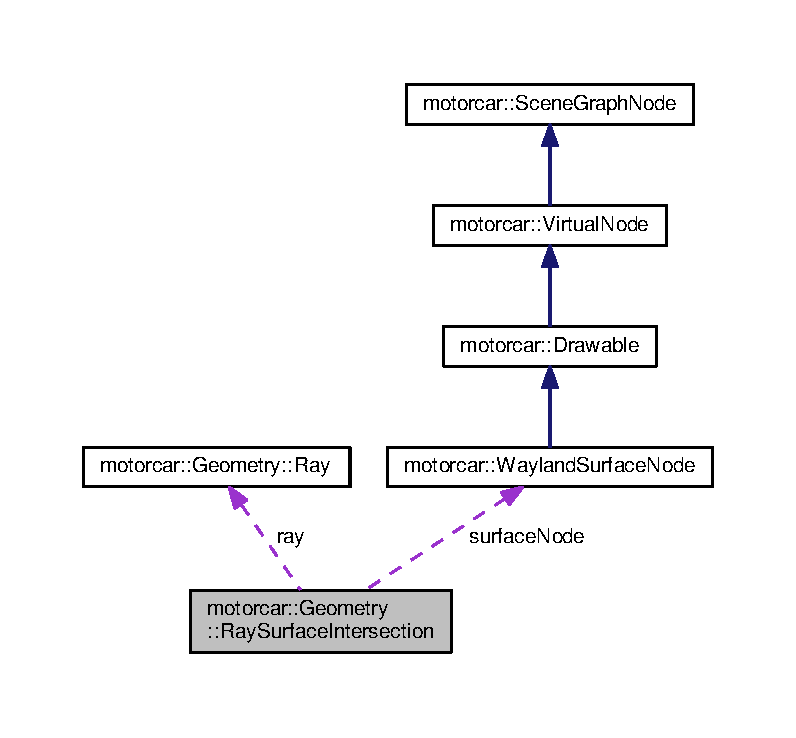
\includegraphics[height=550pt]{structmotorcar_1_1Geometry_1_1RaySurfaceIntersection__coll__graph}
\end{center}
\end{figure}
\subsection*{Public Member Functions}
\begin{DoxyCompactItemize}
\item 
\hyperlink{structmotorcar_1_1Geometry_1_1RaySurfaceIntersection_a25998175e122ecae30e93f823b3b84e4}{Ray\-Surface\-Intersection} (\hyperlink{classmotorcar_1_1WaylandSurfaceNode}{Wayland\-Surface\-Node} $\ast$\hyperlink{structmotorcar_1_1Geometry_1_1RaySurfaceIntersection_aaea662da642316b521721a5dcff0a280}{surface\-Node}, glm\-::vec2 \hyperlink{structmotorcar_1_1Geometry_1_1RaySurfaceIntersection_abb64ad1bdb4385d23970b1c7ecd4afaa}{surface\-Local\-Coordinates}, const \hyperlink{structmotorcar_1_1Geometry_1_1Ray}{Geometry\-::\-Ray} \&\hyperlink{structmotorcar_1_1Geometry_1_1RaySurfaceIntersection_a2e53423ad071c4587aac822ee6aa3de9}{ray}, float \hyperlink{structmotorcar_1_1Geometry_1_1RaySurfaceIntersection_af32545772aead85519b20869fbc34284}{t})
\end{DoxyCompactItemize}
\subsection*{Public Attributes}
\begin{DoxyCompactItemize}
\item 
\hyperlink{classmotorcar_1_1WaylandSurfaceNode}{Wayland\-Surface\-Node} $\ast$ \hyperlink{structmotorcar_1_1Geometry_1_1RaySurfaceIntersection_aaea662da642316b521721a5dcff0a280}{surface\-Node}
\item 
glm\-::vec2 \hyperlink{structmotorcar_1_1Geometry_1_1RaySurfaceIntersection_abb64ad1bdb4385d23970b1c7ecd4afaa}{surface\-Local\-Coordinates}
\item 
\hyperlink{structmotorcar_1_1Geometry_1_1Ray}{Geometry\-::\-Ray} \hyperlink{structmotorcar_1_1Geometry_1_1RaySurfaceIntersection_a2e53423ad071c4587aac822ee6aa3de9}{ray}
\item 
float \hyperlink{structmotorcar_1_1Geometry_1_1RaySurfaceIntersection_af32545772aead85519b20869fbc34284}{t}
\end{DoxyCompactItemize}


\subsection{Constructor \& Destructor Documentation}
\hypertarget{structmotorcar_1_1Geometry_1_1RaySurfaceIntersection_a25998175e122ecae30e93f823b3b84e4}{\index{motorcar\-::\-Geometry\-::\-Ray\-Surface\-Intersection@{motorcar\-::\-Geometry\-::\-Ray\-Surface\-Intersection}!Ray\-Surface\-Intersection@{Ray\-Surface\-Intersection}}
\index{Ray\-Surface\-Intersection@{Ray\-Surface\-Intersection}!motorcar::Geometry::RaySurfaceIntersection@{motorcar\-::\-Geometry\-::\-Ray\-Surface\-Intersection}}
\subsubsection[{Ray\-Surface\-Intersection}]{\setlength{\rightskip}{0pt plus 5cm}Geometry\-::\-Ray\-Surface\-Intersection\-::\-Ray\-Surface\-Intersection (
\begin{DoxyParamCaption}
\item[{{\bf Wayland\-Surface\-Node} $\ast$}]{surface\-Node, }
\item[{glm\-::vec2}]{surface\-Local\-Coordinates, }
\item[{const {\bf Geometry\-::\-Ray} \&}]{ray, }
\item[{float}]{t}
\end{DoxyParamCaption}
)}}\label{structmotorcar_1_1Geometry_1_1RaySurfaceIntersection_a25998175e122ecae30e93f823b3b84e4}


\subsection{Member Data Documentation}
\hypertarget{structmotorcar_1_1Geometry_1_1RaySurfaceIntersection_a2e53423ad071c4587aac822ee6aa3de9}{\index{motorcar\-::\-Geometry\-::\-Ray\-Surface\-Intersection@{motorcar\-::\-Geometry\-::\-Ray\-Surface\-Intersection}!ray@{ray}}
\index{ray@{ray}!motorcar::Geometry::RaySurfaceIntersection@{motorcar\-::\-Geometry\-::\-Ray\-Surface\-Intersection}}
\subsubsection[{ray}]{\setlength{\rightskip}{0pt plus 5cm}{\bf Geometry\-::\-Ray} motorcar\-::\-Geometry\-::\-Ray\-Surface\-Intersection\-::ray}}\label{structmotorcar_1_1Geometry_1_1RaySurfaceIntersection_a2e53423ad071c4587aac822ee6aa3de9}
\hypertarget{structmotorcar_1_1Geometry_1_1RaySurfaceIntersection_abb64ad1bdb4385d23970b1c7ecd4afaa}{\index{motorcar\-::\-Geometry\-::\-Ray\-Surface\-Intersection@{motorcar\-::\-Geometry\-::\-Ray\-Surface\-Intersection}!surface\-Local\-Coordinates@{surface\-Local\-Coordinates}}
\index{surface\-Local\-Coordinates@{surface\-Local\-Coordinates}!motorcar::Geometry::RaySurfaceIntersection@{motorcar\-::\-Geometry\-::\-Ray\-Surface\-Intersection}}
\subsubsection[{surface\-Local\-Coordinates}]{\setlength{\rightskip}{0pt plus 5cm}glm\-::vec2 motorcar\-::\-Geometry\-::\-Ray\-Surface\-Intersection\-::surface\-Local\-Coordinates}}\label{structmotorcar_1_1Geometry_1_1RaySurfaceIntersection_abb64ad1bdb4385d23970b1c7ecd4afaa}
\hypertarget{structmotorcar_1_1Geometry_1_1RaySurfaceIntersection_aaea662da642316b521721a5dcff0a280}{\index{motorcar\-::\-Geometry\-::\-Ray\-Surface\-Intersection@{motorcar\-::\-Geometry\-::\-Ray\-Surface\-Intersection}!surface\-Node@{surface\-Node}}
\index{surface\-Node@{surface\-Node}!motorcar::Geometry::RaySurfaceIntersection@{motorcar\-::\-Geometry\-::\-Ray\-Surface\-Intersection}}
\subsubsection[{surface\-Node}]{\setlength{\rightskip}{0pt plus 5cm}{\bf Wayland\-Surface\-Node}$\ast$ motorcar\-::\-Geometry\-::\-Ray\-Surface\-Intersection\-::surface\-Node}}\label{structmotorcar_1_1Geometry_1_1RaySurfaceIntersection_aaea662da642316b521721a5dcff0a280}
\hypertarget{structmotorcar_1_1Geometry_1_1RaySurfaceIntersection_af32545772aead85519b20869fbc34284}{\index{motorcar\-::\-Geometry\-::\-Ray\-Surface\-Intersection@{motorcar\-::\-Geometry\-::\-Ray\-Surface\-Intersection}!t@{t}}
\index{t@{t}!motorcar::Geometry::RaySurfaceIntersection@{motorcar\-::\-Geometry\-::\-Ray\-Surface\-Intersection}}
\subsubsection[{t}]{\setlength{\rightskip}{0pt plus 5cm}float motorcar\-::\-Geometry\-::\-Ray\-Surface\-Intersection\-::t}}\label{structmotorcar_1_1Geometry_1_1RaySurfaceIntersection_af32545772aead85519b20869fbc34284}


The documentation for this struct was generated from the following files\-:\begin{DoxyCompactItemize}
\item 
/home/dave/thesis/qtwayland-\/motorcar-\/compositor/motorcar/src/\hyperlink{geometry_8h}{geometry.\-h}\item 
/home/dave/thesis/qtwayland-\/motorcar-\/compositor/motorcar/src/\hyperlink{geometry_8cpp}{geometry.\-cpp}\end{DoxyCompactItemize}

\hypertarget{classmotorcar_1_1RenderToTextureDisplay}{\section{motorcar\-:\-:Render\-To\-Texture\-Display Class Reference}
\label{classmotorcar_1_1RenderToTextureDisplay}\index{motorcar\-::\-Render\-To\-Texture\-Display@{motorcar\-::\-Render\-To\-Texture\-Display}}
}


{\ttfamily \#include $<$rendertotexturedisplay.\-h$>$}



Inheritance diagram for motorcar\-:\-:Render\-To\-Texture\-Display\-:
\nopagebreak
\begin{figure}[H]
\begin{center}
\leavevmode
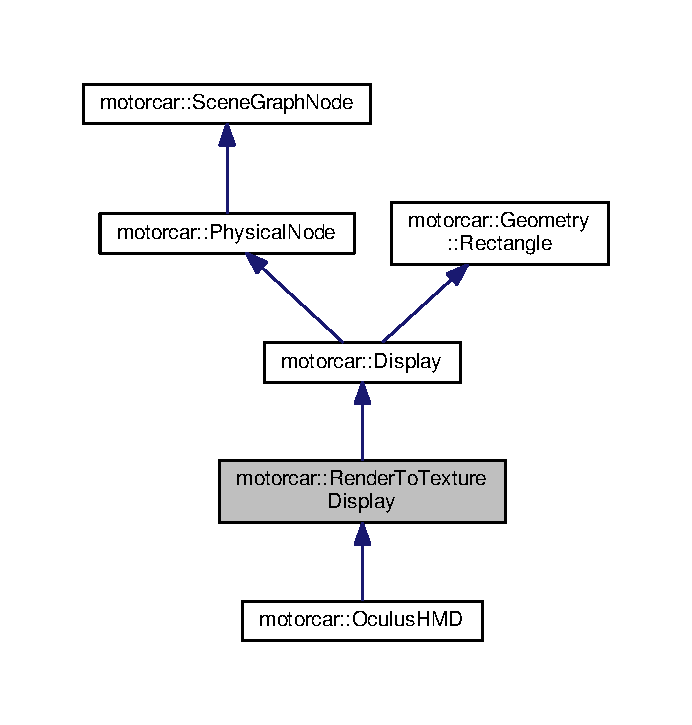
\includegraphics[width=332pt]{classmotorcar_1_1RenderToTextureDisplay__inherit__graph}
\end{center}
\end{figure}


Collaboration diagram for motorcar\-:\-:Render\-To\-Texture\-Display\-:
\nopagebreak
\begin{figure}[H]
\begin{center}
\leavevmode
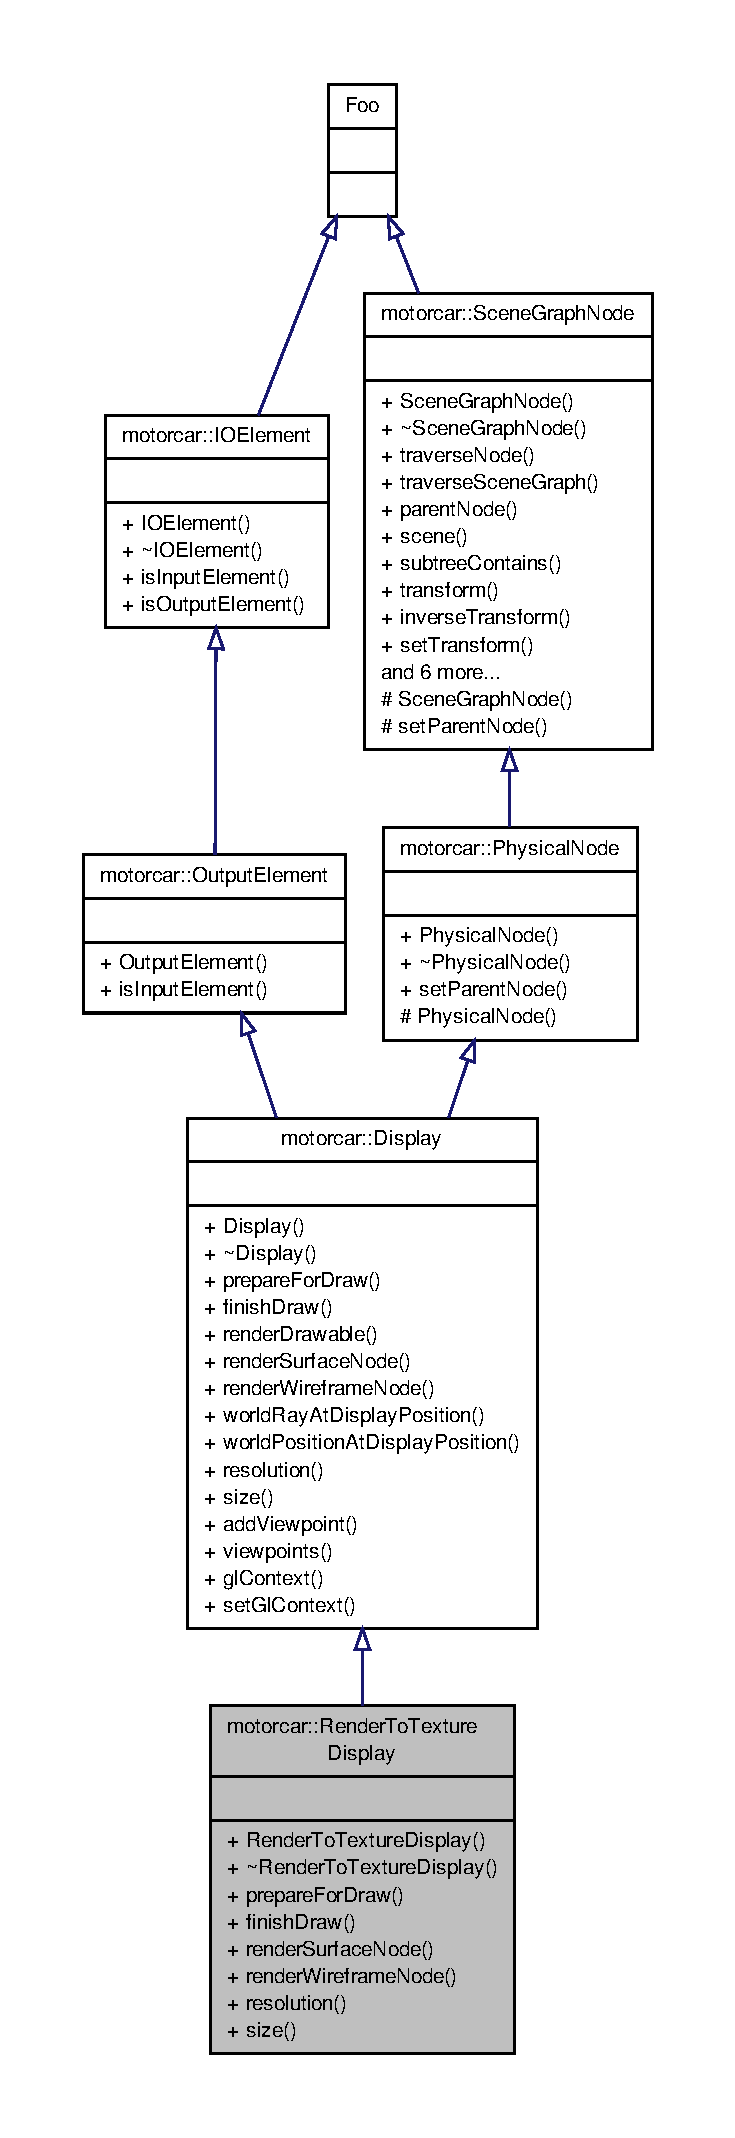
\includegraphics[width=332pt]{classmotorcar_1_1RenderToTextureDisplay__coll__graph}
\end{center}
\end{figure}
\subsection*{Public Member Functions}
\begin{DoxyCompactItemize}
\item 
\hyperlink{classmotorcar_1_1RenderToTextureDisplay_a9c79fc8d2429e8b15c0353a5a9fce42f}{Render\-To\-Texture\-Display} (float scale, glm\-::vec4 distortion\-K, \hyperlink{classmotorcar_1_1OpenGLContext}{Open\-G\-L\-Context} $\ast$\hyperlink{classmotorcar_1_1Display_a884dd0b78dbecee82a33eb6d26a2a403}{gl\-Context}, glm\-::vec2 display\-Dimensions, \hyperlink{classmotorcar_1_1PhysicalNode}{Physical\-Node} $\ast$parent, const glm\-::mat4 \&\hyperlink{classmotorcar_1_1SceneGraphNode_ad96e79fdd739ac8223a3128003be391a}{transform}=glm\-::mat4())
\item 
virtual \hyperlink{classmotorcar_1_1RenderToTextureDisplay_a9cb7b619ef7450f8c208961d83671998}{$\sim$\-Render\-To\-Texture\-Display} ()
\item 
virtual void \hyperlink{classmotorcar_1_1RenderToTextureDisplay_abdf6861fe69ada64fafd0a7713391bed}{prepare\-For\-Draw} () override
\item 
virtual void \hyperlink{classmotorcar_1_1RenderToTextureDisplay_a5a312b98ac49013155797e814e6cf69e}{finish\-Draw} () override
\item 
virtual glm\-::ivec2 \hyperlink{classmotorcar_1_1RenderToTextureDisplay_a2e10611cf3fd629a4d962988642ad5b2}{size} () override
\item 
virtual glm\-::vec2 \hyperlink{classmotorcar_1_1RenderToTextureDisplay_a0ede4d9139786227f2c5d87bbbb9dcfa}{dimensions} () const override
\item 
virtual G\-Luint \hyperlink{classmotorcar_1_1RenderToTextureDisplay_a8c928fb82c28d4785c58a1bd321e0ca6}{active\-Frame\-Buffer} () const override
\item 
virtual G\-Luint \hyperlink{classmotorcar_1_1RenderToTextureDisplay_a4dca5858105e2ee493ef0c49e62c37d4}{depth\-Buffer\-Texture} () const override
\end{DoxyCompactItemize}
\subsection*{Additional Inherited Members}


\subsection{Constructor \& Destructor Documentation}
\hypertarget{classmotorcar_1_1RenderToTextureDisplay_a9c79fc8d2429e8b15c0353a5a9fce42f}{\index{motorcar\-::\-Render\-To\-Texture\-Display@{motorcar\-::\-Render\-To\-Texture\-Display}!Render\-To\-Texture\-Display@{Render\-To\-Texture\-Display}}
\index{Render\-To\-Texture\-Display@{Render\-To\-Texture\-Display}!motorcar::RenderToTextureDisplay@{motorcar\-::\-Render\-To\-Texture\-Display}}
\subsubsection[{Render\-To\-Texture\-Display}]{\setlength{\rightskip}{0pt plus 5cm}Render\-To\-Texture\-Display\-::\-Render\-To\-Texture\-Display (
\begin{DoxyParamCaption}
\item[{float}]{scale, }
\item[{glm\-::vec4}]{distortion\-K, }
\item[{{\bf Open\-G\-L\-Context} $\ast$}]{gl\-Context, }
\item[{glm\-::vec2}]{display\-Dimensions, }
\item[{{\bf Physical\-Node} $\ast$}]{parent, }
\item[{const glm\-::mat4 \&}]{transform = {\ttfamily glm\-:\-:mat4()}}
\end{DoxyParamCaption}
)}}\label{classmotorcar_1_1RenderToTextureDisplay_a9c79fc8d2429e8b15c0353a5a9fce42f}
\hypertarget{classmotorcar_1_1RenderToTextureDisplay_a9cb7b619ef7450f8c208961d83671998}{\index{motorcar\-::\-Render\-To\-Texture\-Display@{motorcar\-::\-Render\-To\-Texture\-Display}!$\sim$\-Render\-To\-Texture\-Display@{$\sim$\-Render\-To\-Texture\-Display}}
\index{$\sim$\-Render\-To\-Texture\-Display@{$\sim$\-Render\-To\-Texture\-Display}!motorcar::RenderToTextureDisplay@{motorcar\-::\-Render\-To\-Texture\-Display}}
\subsubsection[{$\sim$\-Render\-To\-Texture\-Display}]{\setlength{\rightskip}{0pt plus 5cm}Render\-To\-Texture\-Display\-::$\sim$\-Render\-To\-Texture\-Display (
\begin{DoxyParamCaption}
{}
\end{DoxyParamCaption}
)\hspace{0.3cm}{\ttfamily [virtual]}}}\label{classmotorcar_1_1RenderToTextureDisplay_a9cb7b619ef7450f8c208961d83671998}


\subsection{Member Function Documentation}
\hypertarget{classmotorcar_1_1RenderToTextureDisplay_a8c928fb82c28d4785c58a1bd321e0ca6}{\index{motorcar\-::\-Render\-To\-Texture\-Display@{motorcar\-::\-Render\-To\-Texture\-Display}!active\-Frame\-Buffer@{active\-Frame\-Buffer}}
\index{active\-Frame\-Buffer@{active\-Frame\-Buffer}!motorcar::RenderToTextureDisplay@{motorcar\-::\-Render\-To\-Texture\-Display}}
\subsubsection[{active\-Frame\-Buffer}]{\setlength{\rightskip}{0pt plus 5cm}G\-Luint Render\-To\-Texture\-Display\-::active\-Frame\-Buffer (
\begin{DoxyParamCaption}
{}
\end{DoxyParamCaption}
) const\hspace{0.3cm}{\ttfamily [override]}, {\ttfamily [virtual]}}}\label{classmotorcar_1_1RenderToTextureDisplay_a8c928fb82c28d4785c58a1bd321e0ca6}


Reimplemented from \hyperlink{classmotorcar_1_1Display_a7318ea219f098a3a8b412dcec0745334}{motorcar\-::\-Display}.

\hypertarget{classmotorcar_1_1RenderToTextureDisplay_a4dca5858105e2ee493ef0c49e62c37d4}{\index{motorcar\-::\-Render\-To\-Texture\-Display@{motorcar\-::\-Render\-To\-Texture\-Display}!depth\-Buffer\-Texture@{depth\-Buffer\-Texture}}
\index{depth\-Buffer\-Texture@{depth\-Buffer\-Texture}!motorcar::RenderToTextureDisplay@{motorcar\-::\-Render\-To\-Texture\-Display}}
\subsubsection[{depth\-Buffer\-Texture}]{\setlength{\rightskip}{0pt plus 5cm}G\-Luint Render\-To\-Texture\-Display\-::depth\-Buffer\-Texture (
\begin{DoxyParamCaption}
{}
\end{DoxyParamCaption}
) const\hspace{0.3cm}{\ttfamily [override]}, {\ttfamily [virtual]}}}\label{classmotorcar_1_1RenderToTextureDisplay_a4dca5858105e2ee493ef0c49e62c37d4}


Reimplemented from \hyperlink{classmotorcar_1_1Display_a90c69af93ca9d9fff26839fce0e90d53}{motorcar\-::\-Display}.

\hypertarget{classmotorcar_1_1RenderToTextureDisplay_a0ede4d9139786227f2c5d87bbbb9dcfa}{\index{motorcar\-::\-Render\-To\-Texture\-Display@{motorcar\-::\-Render\-To\-Texture\-Display}!dimensions@{dimensions}}
\index{dimensions@{dimensions}!motorcar::RenderToTextureDisplay@{motorcar\-::\-Render\-To\-Texture\-Display}}
\subsubsection[{dimensions}]{\setlength{\rightskip}{0pt plus 5cm}glm\-::vec2 Render\-To\-Texture\-Display\-::dimensions (
\begin{DoxyParamCaption}
{}
\end{DoxyParamCaption}
) const\hspace{0.3cm}{\ttfamily [override]}, {\ttfamily [virtual]}}}\label{classmotorcar_1_1RenderToTextureDisplay_a0ede4d9139786227f2c5d87bbbb9dcfa}


Reimplemented from \hyperlink{classmotorcar_1_1Display_aea90a885c5f3a124a3581bbeeeb4a425}{motorcar\-::\-Display}.

\hypertarget{classmotorcar_1_1RenderToTextureDisplay_a5a312b98ac49013155797e814e6cf69e}{\index{motorcar\-::\-Render\-To\-Texture\-Display@{motorcar\-::\-Render\-To\-Texture\-Display}!finish\-Draw@{finish\-Draw}}
\index{finish\-Draw@{finish\-Draw}!motorcar::RenderToTextureDisplay@{motorcar\-::\-Render\-To\-Texture\-Display}}
\subsubsection[{finish\-Draw}]{\setlength{\rightskip}{0pt plus 5cm}void Render\-To\-Texture\-Display\-::finish\-Draw (
\begin{DoxyParamCaption}
{}
\end{DoxyParamCaption}
)\hspace{0.3cm}{\ttfamily [override]}, {\ttfamily [virtual]}}}\label{classmotorcar_1_1RenderToTextureDisplay_a5a312b98ac49013155797e814e6cf69e}


Reimplemented from \hyperlink{classmotorcar_1_1Display_a162b721d9c039887fc37b6a090ff1074}{motorcar\-::\-Display}.

\hypertarget{classmotorcar_1_1RenderToTextureDisplay_abdf6861fe69ada64fafd0a7713391bed}{\index{motorcar\-::\-Render\-To\-Texture\-Display@{motorcar\-::\-Render\-To\-Texture\-Display}!prepare\-For\-Draw@{prepare\-For\-Draw}}
\index{prepare\-For\-Draw@{prepare\-For\-Draw}!motorcar::RenderToTextureDisplay@{motorcar\-::\-Render\-To\-Texture\-Display}}
\subsubsection[{prepare\-For\-Draw}]{\setlength{\rightskip}{0pt plus 5cm}void Render\-To\-Texture\-Display\-::prepare\-For\-Draw (
\begin{DoxyParamCaption}
{}
\end{DoxyParamCaption}
)\hspace{0.3cm}{\ttfamily [override]}, {\ttfamily [virtual]}}}\label{classmotorcar_1_1RenderToTextureDisplay_abdf6861fe69ada64fafd0a7713391bed}


Reimplemented from \hyperlink{classmotorcar_1_1Display_a0b26d9162f4f8f0848af408791be631c}{motorcar\-::\-Display}.



Reimplemented in \hyperlink{classmotorcar_1_1OculusHMD_ae9834ea50d728809532b7a48f7ed1738}{motorcar\-::\-Oculus\-H\-M\-D}.

\hypertarget{classmotorcar_1_1RenderToTextureDisplay_a2e10611cf3fd629a4d962988642ad5b2}{\index{motorcar\-::\-Render\-To\-Texture\-Display@{motorcar\-::\-Render\-To\-Texture\-Display}!size@{size}}
\index{size@{size}!motorcar::RenderToTextureDisplay@{motorcar\-::\-Render\-To\-Texture\-Display}}
\subsubsection[{size}]{\setlength{\rightskip}{0pt plus 5cm}glm\-::ivec2 Render\-To\-Texture\-Display\-::size (
\begin{DoxyParamCaption}
{}
\end{DoxyParamCaption}
)\hspace{0.3cm}{\ttfamily [override]}, {\ttfamily [virtual]}}}\label{classmotorcar_1_1RenderToTextureDisplay_a2e10611cf3fd629a4d962988642ad5b2}


Reimplemented from \hyperlink{classmotorcar_1_1Display_a58a94b72684d5b8569a9169591f7613e}{motorcar\-::\-Display}.



The documentation for this class was generated from the following files\-:\begin{DoxyCompactItemize}
\item 
/home/dave/thesis/motorcar/src/compositor/scenegraph/output/display/\hyperlink{rendertotexturedisplay_8h}{rendertotexturedisplay.\-h}\item 
/home/dave/thesis/motorcar/src/compositor/scenegraph/output/display/\hyperlink{rendertotexturedisplay_8cpp}{rendertotexturedisplay.\-cpp}\end{DoxyCompactItemize}

\hypertarget{classmotorcar_1_1Scene}{\section{motorcar\-:\-:Scene Class Reference}
\label{classmotorcar_1_1Scene}\index{motorcar\-::\-Scene@{motorcar\-::\-Scene}}
}


{\ttfamily \#include $<$scene.\-h$>$}



Inheritance diagram for motorcar\-:\-:Scene\-:
\nopagebreak
\begin{figure}[H]
\begin{center}
\leavevmode
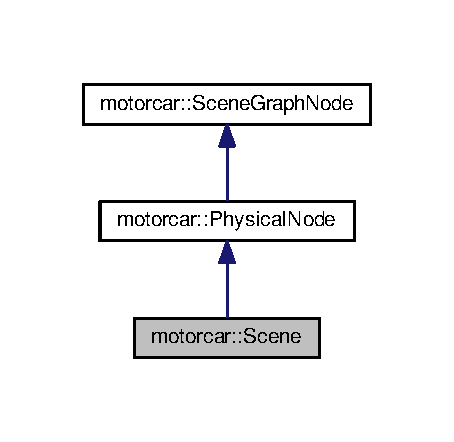
\includegraphics[height=550pt]{classmotorcar_1_1Scene__inherit__graph}
\end{center}
\end{figure}


Collaboration diagram for motorcar\-:\-:Scene\-:
\nopagebreak
\begin{figure}[H]
\begin{center}
\leavevmode
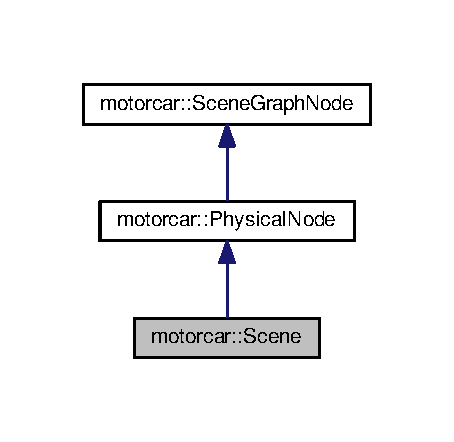
\includegraphics[height=550pt]{classmotorcar_1_1Scene__coll__graph}
\end{center}
\end{figure}
\subsection*{Public Member Functions}
\begin{DoxyCompactItemize}
\item 
\hyperlink{classmotorcar_1_1Scene_ad10176d75a9cc0da56626f682d083507}{Scene} ()
\item 
virtual \hyperlink{classmotorcar_1_1Scene_a07ad90930bf4792b88c8ce8b6800df4d}{$\sim$\-Scene} ()
\item 
virtual void \hyperlink{classmotorcar_1_1Scene_a11f9f856df5db6db78760cae5dc02079}{notify\-Node\-Added} (\hyperlink{classmotorcar_1_1SceneGraphNode}{Scene\-Graph\-Node} $\ast$node)
\item 
void \hyperlink{classmotorcar_1_1Scene_a3482161400b2f552307cc70812b128a9}{add\-Display} (\hyperlink{classmotorcar_1_1Display}{Display} $\ast$display)
\item 
std\-::vector$<$ \hyperlink{classmotorcar_1_1Display}{Display} $\ast$ $>$ \hyperlink{classmotorcar_1_1Scene_a1c09a0e3e55f1dd870d5c3001890afa9}{displays} () const 
\item 
void \hyperlink{classmotorcar_1_1Scene_ae8c9484b131cf87e8b1ebca4500343ae}{draw} (long delta\-Millis)
\item 
\hyperlink{classmotorcar_1_1WaylandSurfaceNode}{Wayland\-Surface\-Node} $\ast$ \hyperlink{classmotorcar_1_1Scene_a124b886baea9b583feb477202c9038a2}{cursor\-Node} () const 
\item 
void \hyperlink{classmotorcar_1_1Scene_a76a501d972979ba633dd0e38b022ab9b}{set\-Cursor\-Node} (\hyperlink{classmotorcar_1_1WaylandSurfaceNode}{Wayland\-Surface\-Node} $\ast$\hyperlink{classmotorcar_1_1Scene_a124b886baea9b583feb477202c9038a2}{cursor\-Node})
\item 
glm\-::ivec2 \hyperlink{classmotorcar_1_1Scene_abdb097ab9a2927b447b2eee485d19d6e}{cursor\-Hotspot} () const 
\item 
void \hyperlink{classmotorcar_1_1Scene_aba832b6a205b06b9d266ee3302ff86f4}{set\-Cursor\-Hotspot} (const glm\-::ivec2 \&\hyperlink{classmotorcar_1_1Scene_abdb097ab9a2927b447b2eee485d19d6e}{cursor\-Hotspot})
\end{DoxyCompactItemize}
\subsection*{Additional Inherited Members}


\subsection{Constructor \& Destructor Documentation}
\hypertarget{classmotorcar_1_1Scene_ad10176d75a9cc0da56626f682d083507}{\index{motorcar\-::\-Scene@{motorcar\-::\-Scene}!Scene@{Scene}}
\index{Scene@{Scene}!motorcar::Scene@{motorcar\-::\-Scene}}
\subsubsection[{Scene}]{\setlength{\rightskip}{0pt plus 5cm}Scene\-::\-Scene (
\begin{DoxyParamCaption}
{}
\end{DoxyParamCaption}
)}}\label{classmotorcar_1_1Scene_ad10176d75a9cc0da56626f682d083507}
\hypertarget{classmotorcar_1_1Scene_a07ad90930bf4792b88c8ce8b6800df4d}{\index{motorcar\-::\-Scene@{motorcar\-::\-Scene}!$\sim$\-Scene@{$\sim$\-Scene}}
\index{$\sim$\-Scene@{$\sim$\-Scene}!motorcar::Scene@{motorcar\-::\-Scene}}
\subsubsection[{$\sim$\-Scene}]{\setlength{\rightskip}{0pt plus 5cm}virtual motorcar\-::\-Scene\-::$\sim$\-Scene (
\begin{DoxyParamCaption}
{}
\end{DoxyParamCaption}
)\hspace{0.3cm}{\ttfamily [inline]}, {\ttfamily [virtual]}}}\label{classmotorcar_1_1Scene_a07ad90930bf4792b88c8ce8b6800df4d}


\subsection{Member Function Documentation}
\hypertarget{classmotorcar_1_1Scene_a3482161400b2f552307cc70812b128a9}{\index{motorcar\-::\-Scene@{motorcar\-::\-Scene}!add\-Display@{add\-Display}}
\index{add\-Display@{add\-Display}!motorcar::Scene@{motorcar\-::\-Scene}}
\subsubsection[{add\-Display}]{\setlength{\rightskip}{0pt plus 5cm}void Scene\-::add\-Display (
\begin{DoxyParamCaption}
\item[{{\bf Display} $\ast$}]{display}
\end{DoxyParamCaption}
)}}\label{classmotorcar_1_1Scene_a3482161400b2f552307cc70812b128a9}
\hypertarget{classmotorcar_1_1Scene_abdb097ab9a2927b447b2eee485d19d6e}{\index{motorcar\-::\-Scene@{motorcar\-::\-Scene}!cursor\-Hotspot@{cursor\-Hotspot}}
\index{cursor\-Hotspot@{cursor\-Hotspot}!motorcar::Scene@{motorcar\-::\-Scene}}
\subsubsection[{cursor\-Hotspot}]{\setlength{\rightskip}{0pt plus 5cm}glm\-::ivec2 Scene\-::cursor\-Hotspot (
\begin{DoxyParamCaption}
{}
\end{DoxyParamCaption}
) const}}\label{classmotorcar_1_1Scene_abdb097ab9a2927b447b2eee485d19d6e}
\hypertarget{classmotorcar_1_1Scene_a124b886baea9b583feb477202c9038a2}{\index{motorcar\-::\-Scene@{motorcar\-::\-Scene}!cursor\-Node@{cursor\-Node}}
\index{cursor\-Node@{cursor\-Node}!motorcar::Scene@{motorcar\-::\-Scene}}
\subsubsection[{cursor\-Node}]{\setlength{\rightskip}{0pt plus 5cm}{\bf Wayland\-Surface\-Node} $\ast$ Scene\-::cursor\-Node (
\begin{DoxyParamCaption}
{}
\end{DoxyParamCaption}
) const}}\label{classmotorcar_1_1Scene_a124b886baea9b583feb477202c9038a2}
\hypertarget{classmotorcar_1_1Scene_a1c09a0e3e55f1dd870d5c3001890afa9}{\index{motorcar\-::\-Scene@{motorcar\-::\-Scene}!displays@{displays}}
\index{displays@{displays}!motorcar::Scene@{motorcar\-::\-Scene}}
\subsubsection[{displays}]{\setlength{\rightskip}{0pt plus 5cm}std\-::vector$<$ {\bf Display} $\ast$ $>$ Scene\-::displays (
\begin{DoxyParamCaption}
{}
\end{DoxyParamCaption}
) const}}\label{classmotorcar_1_1Scene_a1c09a0e3e55f1dd870d5c3001890afa9}
\hypertarget{classmotorcar_1_1Scene_ae8c9484b131cf87e8b1ebca4500343ae}{\index{motorcar\-::\-Scene@{motorcar\-::\-Scene}!draw@{draw}}
\index{draw@{draw}!motorcar::Scene@{motorcar\-::\-Scene}}
\subsubsection[{draw}]{\setlength{\rightskip}{0pt plus 5cm}void Scene\-::draw (
\begin{DoxyParamCaption}
\item[{long}]{delta\-Millis}
\end{DoxyParamCaption}
)}}\label{classmotorcar_1_1Scene_ae8c9484b131cf87e8b1ebca4500343ae}
\hypertarget{classmotorcar_1_1Scene_a11f9f856df5db6db78760cae5dc02079}{\index{motorcar\-::\-Scene@{motorcar\-::\-Scene}!notify\-Node\-Added@{notify\-Node\-Added}}
\index{notify\-Node\-Added@{notify\-Node\-Added}!motorcar::Scene@{motorcar\-::\-Scene}}
\subsubsection[{notify\-Node\-Added}]{\setlength{\rightskip}{0pt plus 5cm}void Scene\-::notify\-Node\-Added (
\begin{DoxyParamCaption}
\item[{{\bf Scene\-Graph\-Node} $\ast$}]{node}
\end{DoxyParamCaption}
)\hspace{0.3cm}{\ttfamily [virtual]}}}\label{classmotorcar_1_1Scene_a11f9f856df5db6db78760cae5dc02079}
\hypertarget{classmotorcar_1_1Scene_aba832b6a205b06b9d266ee3302ff86f4}{\index{motorcar\-::\-Scene@{motorcar\-::\-Scene}!set\-Cursor\-Hotspot@{set\-Cursor\-Hotspot}}
\index{set\-Cursor\-Hotspot@{set\-Cursor\-Hotspot}!motorcar::Scene@{motorcar\-::\-Scene}}
\subsubsection[{set\-Cursor\-Hotspot}]{\setlength{\rightskip}{0pt plus 5cm}void Scene\-::set\-Cursor\-Hotspot (
\begin{DoxyParamCaption}
\item[{const glm\-::ivec2 \&}]{cursor\-Hotspot}
\end{DoxyParamCaption}
)}}\label{classmotorcar_1_1Scene_aba832b6a205b06b9d266ee3302ff86f4}
\hypertarget{classmotorcar_1_1Scene_a76a501d972979ba633dd0e38b022ab9b}{\index{motorcar\-::\-Scene@{motorcar\-::\-Scene}!set\-Cursor\-Node@{set\-Cursor\-Node}}
\index{set\-Cursor\-Node@{set\-Cursor\-Node}!motorcar::Scene@{motorcar\-::\-Scene}}
\subsubsection[{set\-Cursor\-Node}]{\setlength{\rightskip}{0pt plus 5cm}void Scene\-::set\-Cursor\-Node (
\begin{DoxyParamCaption}
\item[{{\bf Wayland\-Surface\-Node} $\ast$}]{cursor\-Node}
\end{DoxyParamCaption}
)}}\label{classmotorcar_1_1Scene_a76a501d972979ba633dd0e38b022ab9b}


The documentation for this class was generated from the following files\-:\begin{DoxyCompactItemize}
\item 
/home/dave/thesis/qtwayland-\/motorcar-\/compositor/motorcar/src/scenegraph/\hyperlink{scene_8h}{scene.\-h}\item 
/home/dave/thesis/qtwayland-\/motorcar-\/compositor/motorcar/src/scenegraph/\hyperlink{scene_8cpp}{scene.\-cpp}\end{DoxyCompactItemize}

\hypertarget{classmotorcar_1_1SceneGraphNode}{\section{motorcar\-:\-:Scene\-Graph\-Node Class Reference}
\label{classmotorcar_1_1SceneGraphNode}\index{motorcar\-::\-Scene\-Graph\-Node@{motorcar\-::\-Scene\-Graph\-Node}}
}


{\ttfamily \#include $<$scenegraphnode.\-h$>$}



Inheritance diagram for motorcar\-:\-:Scene\-Graph\-Node\-:
\nopagebreak
\begin{figure}[H]
\begin{center}
\leavevmode
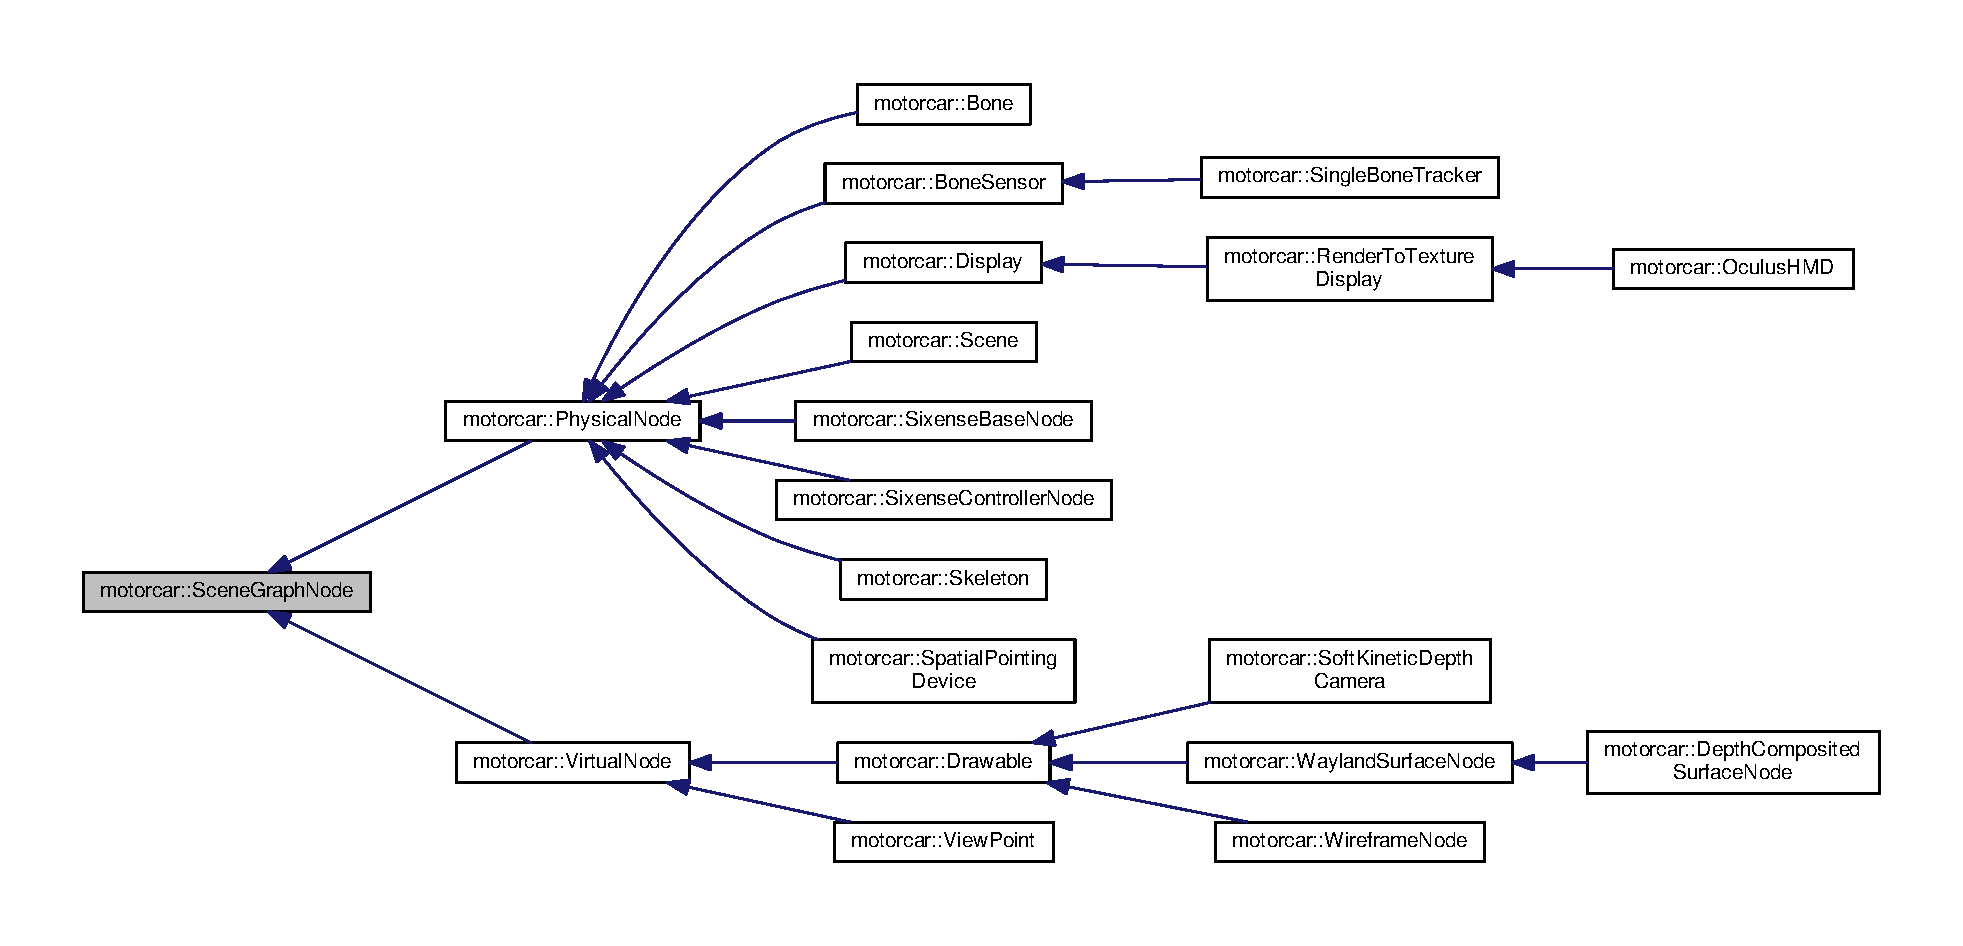
\includegraphics[width=350pt]{classmotorcar_1_1SceneGraphNode__inherit__graph}
\end{center}
\end{figure}


Collaboration diagram for motorcar\-:\-:Scene\-Graph\-Node\-:
\nopagebreak
\begin{figure}[H]
\begin{center}
\leavevmode
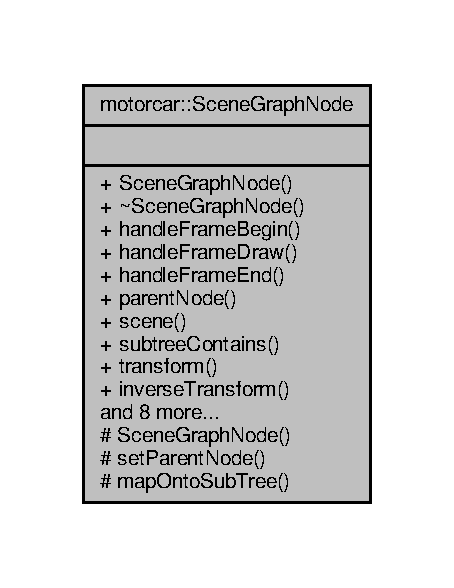
\includegraphics[width=218pt]{classmotorcar_1_1SceneGraphNode__coll__graph}
\end{center}
\end{figure}
\subsection*{Public Member Functions}
\begin{DoxyCompactItemize}
\item 
\hyperlink{classmotorcar_1_1SceneGraphNode_a293d96c3691afbaaba0da114a5e8f433}{Scene\-Graph\-Node} (\hyperlink{classmotorcar_1_1SceneGraphNode}{Scene\-Graph\-Node} $\ast$parent, glm\-::mat4 \hyperlink{classmotorcar_1_1SceneGraphNode_ad96e79fdd739ac8223a3128003be391a}{transform}=glm\-::mat4())
\item 
virtual \hyperlink{classmotorcar_1_1SceneGraphNode_ae81a28adc17e6be945c8279e4af4108c}{$\sim$\-Scene\-Graph\-Node} ()
\item 
virtual void \hyperlink{classmotorcar_1_1SceneGraphNode_aa680a8e89fc8ebd12b784653fb30c29a}{traverse\-Node} (\hyperlink{classmotorcar_1_1Scene}{Scene} $\ast$\hyperlink{classmotorcar_1_1SceneGraphNode_aa14e637ed4ae98f77e28941a4b5cfdd8}{scene}, long delta\-Millis)
\item 
void \hyperlink{classmotorcar_1_1SceneGraphNode_ac1e4d2185a8df5b84af1693a5d72d4fc}{traverse\-Scene\-Graph} (\hyperlink{classmotorcar_1_1Scene}{Scene} $\ast$\hyperlink{classmotorcar_1_1SceneGraphNode_aa14e637ed4ae98f77e28941a4b5cfdd8}{scene}, long delta\-Millis)
\item 
\hyperlink{classmotorcar_1_1SceneGraphNode}{Scene\-Graph\-Node} $\ast$ \hyperlink{classmotorcar_1_1SceneGraphNode_a57dd5826ed6bf15c8a879f5a090c6000}{parent\-Node} () const 
\item 
\hyperlink{classmotorcar_1_1Scene}{Scene} $\ast$ \hyperlink{classmotorcar_1_1SceneGraphNode_aa14e637ed4ae98f77e28941a4b5cfdd8}{scene} ()
\item 
bool \hyperlink{classmotorcar_1_1SceneGraphNode_ac2be631270bc40cb1e070983c30a323f}{subtree\-Contains} (\hyperlink{classmotorcar_1_1SceneGraphNode}{Scene\-Graph\-Node} $\ast$node)
\item 
glm\-::mat4 \hyperlink{classmotorcar_1_1SceneGraphNode_ad96e79fdd739ac8223a3128003be391a}{transform} () const 
\item 
glm\-::mat4 \hyperlink{classmotorcar_1_1SceneGraphNode_af8b8174098f1de1067541f0e3ebec72e}{inverse\-Transform} () const 
\item 
void \hyperlink{classmotorcar_1_1SceneGraphNode_a7cd7700336833efa89c8004e85a1fd61}{set\-Transform} (const glm\-::mat4 \&\hyperlink{classmotorcar_1_1SceneGraphNode_ad96e79fdd739ac8223a3128003be391a}{transform})
\item 
glm\-::mat4 \hyperlink{classmotorcar_1_1SceneGraphNode_a3e7fba2add3f63a65f31996f0ce9c9bf}{world\-Transform} () const 
\item 
glm\-::mat4 \hyperlink{classmotorcar_1_1SceneGraphNode_a10e4fd743e891cef676435c5f5d5467d}{inverse\-World\-Transform} () const 
\item 
void \hyperlink{classmotorcar_1_1SceneGraphNode_ac1a30cbe4af18133b19e6f852c33e30a}{set\-World\-Transform} (const glm\-::mat4 \&\hyperlink{classmotorcar_1_1SceneGraphNode_ad96e79fdd739ac8223a3128003be391a}{transform})
\item 
virtual \\*
\hyperlink{structmotorcar_1_1Geometry_1_1RaySurfaceIntersection}{Geometry\-::\-Ray\-Surface\-Intersection} $\ast$ \hyperlink{classmotorcar_1_1SceneGraphNode_ac268b171317430368fcc7733eab05ae6}{intersect\-With\-Surfaces} (const \hyperlink{structmotorcar_1_1Geometry_1_1Ray}{Geometry\-::\-Ray} \&ray)
\item 
std\-::vector$<$ \hyperlink{classmotorcar_1_1SceneGraphNode}{Scene\-Graph\-Node} $\ast$ $>$ \hyperlink{classmotorcar_1_1SceneGraphNode_a9a0c649390da0918afd58805192ccdca}{child\-Nodes} () const 
\item 
std\-::vector$<$ \hyperlink{classmotorcar_1_1SceneGraphNode}{Scene\-Graph\-Node} $\ast$ $>$ \hyperlink{classmotorcar_1_1SceneGraphNode_aa7ac1c085afbe0fb0b9d5cd578a8c4ef}{nodes\-In\-Subtree} () const 
\end{DoxyCompactItemize}
\subsection*{Protected Member Functions}
\begin{DoxyCompactItemize}
\item 
\hyperlink{classmotorcar_1_1SceneGraphNode_ab9bc5f59ccba332aab918c7b066c309f}{Scene\-Graph\-Node} ()
\item 
void \hyperlink{classmotorcar_1_1SceneGraphNode_a977b156ebcc07018a475b4042de8886a}{set\-Parent\-Node} (\hyperlink{classmotorcar_1_1SceneGraphNode}{Scene\-Graph\-Node} $\ast$parent)
\end{DoxyCompactItemize}


\subsection{Constructor \& Destructor Documentation}
\hypertarget{classmotorcar_1_1SceneGraphNode_a293d96c3691afbaaba0da114a5e8f433}{\index{motorcar\-::\-Scene\-Graph\-Node@{motorcar\-::\-Scene\-Graph\-Node}!Scene\-Graph\-Node@{Scene\-Graph\-Node}}
\index{Scene\-Graph\-Node@{Scene\-Graph\-Node}!motorcar::SceneGraphNode@{motorcar\-::\-Scene\-Graph\-Node}}
\subsubsection[{Scene\-Graph\-Node}]{\setlength{\rightskip}{0pt plus 5cm}Scene\-Graph\-Node\-::\-Scene\-Graph\-Node (
\begin{DoxyParamCaption}
\item[{{\bf Scene\-Graph\-Node} $\ast$}]{parent, }
\item[{glm\-::mat4}]{transform = {\ttfamily glm\-:\-:mat4()}}
\end{DoxyParamCaption}
)}}\label{classmotorcar_1_1SceneGraphNode_a293d96c3691afbaaba0da114a5e8f433}
\hypertarget{classmotorcar_1_1SceneGraphNode_ae81a28adc17e6be945c8279e4af4108c}{\index{motorcar\-::\-Scene\-Graph\-Node@{motorcar\-::\-Scene\-Graph\-Node}!$\sim$\-Scene\-Graph\-Node@{$\sim$\-Scene\-Graph\-Node}}
\index{$\sim$\-Scene\-Graph\-Node@{$\sim$\-Scene\-Graph\-Node}!motorcar::SceneGraphNode@{motorcar\-::\-Scene\-Graph\-Node}}
\subsubsection[{$\sim$\-Scene\-Graph\-Node}]{\setlength{\rightskip}{0pt plus 5cm}Scene\-Graph\-Node\-::$\sim$\-Scene\-Graph\-Node (
\begin{DoxyParamCaption}
{}
\end{DoxyParamCaption}
)\hspace{0.3cm}{\ttfamily [virtual]}}}\label{classmotorcar_1_1SceneGraphNode_ae81a28adc17e6be945c8279e4af4108c}
\hypertarget{classmotorcar_1_1SceneGraphNode_ab9bc5f59ccba332aab918c7b066c309f}{\index{motorcar\-::\-Scene\-Graph\-Node@{motorcar\-::\-Scene\-Graph\-Node}!Scene\-Graph\-Node@{Scene\-Graph\-Node}}
\index{Scene\-Graph\-Node@{Scene\-Graph\-Node}!motorcar::SceneGraphNode@{motorcar\-::\-Scene\-Graph\-Node}}
\subsubsection[{Scene\-Graph\-Node}]{\setlength{\rightskip}{0pt plus 5cm}Scene\-Graph\-Node\-::\-Scene\-Graph\-Node (
\begin{DoxyParamCaption}
{}
\end{DoxyParamCaption}
)\hspace{0.3cm}{\ttfamily [protected]}}}\label{classmotorcar_1_1SceneGraphNode_ab9bc5f59ccba332aab918c7b066c309f}


\subsection{Member Function Documentation}
\hypertarget{classmotorcar_1_1SceneGraphNode_a9a0c649390da0918afd58805192ccdca}{\index{motorcar\-::\-Scene\-Graph\-Node@{motorcar\-::\-Scene\-Graph\-Node}!child\-Nodes@{child\-Nodes}}
\index{child\-Nodes@{child\-Nodes}!motorcar::SceneGraphNode@{motorcar\-::\-Scene\-Graph\-Node}}
\subsubsection[{child\-Nodes}]{\setlength{\rightskip}{0pt plus 5cm}std\-::vector$<$ {\bf Scene\-Graph\-Node} $\ast$ $>$ Scene\-Graph\-Node\-::child\-Nodes (
\begin{DoxyParamCaption}
{}
\end{DoxyParamCaption}
) const}}\label{classmotorcar_1_1SceneGraphNode_a9a0c649390da0918afd58805192ccdca}
\hypertarget{classmotorcar_1_1SceneGraphNode_ac268b171317430368fcc7733eab05ae6}{\index{motorcar\-::\-Scene\-Graph\-Node@{motorcar\-::\-Scene\-Graph\-Node}!intersect\-With\-Surfaces@{intersect\-With\-Surfaces}}
\index{intersect\-With\-Surfaces@{intersect\-With\-Surfaces}!motorcar::SceneGraphNode@{motorcar\-::\-Scene\-Graph\-Node}}
\subsubsection[{intersect\-With\-Surfaces}]{\setlength{\rightskip}{0pt plus 5cm}{\bf Geometry\-::\-Ray\-Surface\-Intersection} $\ast$ Scene\-Graph\-Node\-::intersect\-With\-Surfaces (
\begin{DoxyParamCaption}
\item[{const {\bf Geometry\-::\-Ray} \&}]{ray}
\end{DoxyParamCaption}
)\hspace{0.3cm}{\ttfamily [virtual]}}}\label{classmotorcar_1_1SceneGraphNode_ac268b171317430368fcc7733eab05ae6}


Reimplemented in \hyperlink{classmotorcar_1_1WaylandSurfaceNode_adf71a714d07bb262405a361504a77ea4}{motorcar\-::\-Wayland\-Surface\-Node}.

\hypertarget{classmotorcar_1_1SceneGraphNode_af8b8174098f1de1067541f0e3ebec72e}{\index{motorcar\-::\-Scene\-Graph\-Node@{motorcar\-::\-Scene\-Graph\-Node}!inverse\-Transform@{inverse\-Transform}}
\index{inverse\-Transform@{inverse\-Transform}!motorcar::SceneGraphNode@{motorcar\-::\-Scene\-Graph\-Node}}
\subsubsection[{inverse\-Transform}]{\setlength{\rightskip}{0pt plus 5cm}glm\-::mat4 Scene\-Graph\-Node\-::inverse\-Transform (
\begin{DoxyParamCaption}
{}
\end{DoxyParamCaption}
) const}}\label{classmotorcar_1_1SceneGraphNode_af8b8174098f1de1067541f0e3ebec72e}
\hypertarget{classmotorcar_1_1SceneGraphNode_a10e4fd743e891cef676435c5f5d5467d}{\index{motorcar\-::\-Scene\-Graph\-Node@{motorcar\-::\-Scene\-Graph\-Node}!inverse\-World\-Transform@{inverse\-World\-Transform}}
\index{inverse\-World\-Transform@{inverse\-World\-Transform}!motorcar::SceneGraphNode@{motorcar\-::\-Scene\-Graph\-Node}}
\subsubsection[{inverse\-World\-Transform}]{\setlength{\rightskip}{0pt plus 5cm}glm\-::mat4 Scene\-Graph\-Node\-::inverse\-World\-Transform (
\begin{DoxyParamCaption}
{}
\end{DoxyParamCaption}
) const}}\label{classmotorcar_1_1SceneGraphNode_a10e4fd743e891cef676435c5f5d5467d}
\hypertarget{classmotorcar_1_1SceneGraphNode_aa7ac1c085afbe0fb0b9d5cd578a8c4ef}{\index{motorcar\-::\-Scene\-Graph\-Node@{motorcar\-::\-Scene\-Graph\-Node}!nodes\-In\-Subtree@{nodes\-In\-Subtree}}
\index{nodes\-In\-Subtree@{nodes\-In\-Subtree}!motorcar::SceneGraphNode@{motorcar\-::\-Scene\-Graph\-Node}}
\subsubsection[{nodes\-In\-Subtree}]{\setlength{\rightskip}{0pt plus 5cm}std\-::vector$<$ {\bf Scene\-Graph\-Node} $\ast$ $>$ Scene\-Graph\-Node\-::nodes\-In\-Subtree (
\begin{DoxyParamCaption}
{}
\end{DoxyParamCaption}
) const}}\label{classmotorcar_1_1SceneGraphNode_aa7ac1c085afbe0fb0b9d5cd578a8c4ef}
\hypertarget{classmotorcar_1_1SceneGraphNode_a57dd5826ed6bf15c8a879f5a090c6000}{\index{motorcar\-::\-Scene\-Graph\-Node@{motorcar\-::\-Scene\-Graph\-Node}!parent\-Node@{parent\-Node}}
\index{parent\-Node@{parent\-Node}!motorcar::SceneGraphNode@{motorcar\-::\-Scene\-Graph\-Node}}
\subsubsection[{parent\-Node}]{\setlength{\rightskip}{0pt plus 5cm}{\bf Scene\-Graph\-Node} $\ast$ Scene\-Graph\-Node\-::parent\-Node (
\begin{DoxyParamCaption}
{}
\end{DoxyParamCaption}
) const}}\label{classmotorcar_1_1SceneGraphNode_a57dd5826ed6bf15c8a879f5a090c6000}
\hypertarget{classmotorcar_1_1SceneGraphNode_aa14e637ed4ae98f77e28941a4b5cfdd8}{\index{motorcar\-::\-Scene\-Graph\-Node@{motorcar\-::\-Scene\-Graph\-Node}!scene@{scene}}
\index{scene@{scene}!motorcar::SceneGraphNode@{motorcar\-::\-Scene\-Graph\-Node}}
\subsubsection[{scene}]{\setlength{\rightskip}{0pt plus 5cm}{\bf Scene} $\ast$ Scene\-Graph\-Node\-::scene (
\begin{DoxyParamCaption}
{}
\end{DoxyParamCaption}
)}}\label{classmotorcar_1_1SceneGraphNode_aa14e637ed4ae98f77e28941a4b5cfdd8}
\hypertarget{classmotorcar_1_1SceneGraphNode_a977b156ebcc07018a475b4042de8886a}{\index{motorcar\-::\-Scene\-Graph\-Node@{motorcar\-::\-Scene\-Graph\-Node}!set\-Parent\-Node@{set\-Parent\-Node}}
\index{set\-Parent\-Node@{set\-Parent\-Node}!motorcar::SceneGraphNode@{motorcar\-::\-Scene\-Graph\-Node}}
\subsubsection[{set\-Parent\-Node}]{\setlength{\rightskip}{0pt plus 5cm}void Scene\-Graph\-Node\-::set\-Parent\-Node (
\begin{DoxyParamCaption}
\item[{{\bf Scene\-Graph\-Node} $\ast$}]{parent}
\end{DoxyParamCaption}
)\hspace{0.3cm}{\ttfamily [protected]}}}\label{classmotorcar_1_1SceneGraphNode_a977b156ebcc07018a475b4042de8886a}
\hypertarget{classmotorcar_1_1SceneGraphNode_a7cd7700336833efa89c8004e85a1fd61}{\index{motorcar\-::\-Scene\-Graph\-Node@{motorcar\-::\-Scene\-Graph\-Node}!set\-Transform@{set\-Transform}}
\index{set\-Transform@{set\-Transform}!motorcar::SceneGraphNode@{motorcar\-::\-Scene\-Graph\-Node}}
\subsubsection[{set\-Transform}]{\setlength{\rightskip}{0pt plus 5cm}void Scene\-Graph\-Node\-::set\-Transform (
\begin{DoxyParamCaption}
\item[{const glm\-::mat4 \&}]{transform}
\end{DoxyParamCaption}
)}}\label{classmotorcar_1_1SceneGraphNode_a7cd7700336833efa89c8004e85a1fd61}
\hypertarget{classmotorcar_1_1SceneGraphNode_ac1a30cbe4af18133b19e6f852c33e30a}{\index{motorcar\-::\-Scene\-Graph\-Node@{motorcar\-::\-Scene\-Graph\-Node}!set\-World\-Transform@{set\-World\-Transform}}
\index{set\-World\-Transform@{set\-World\-Transform}!motorcar::SceneGraphNode@{motorcar\-::\-Scene\-Graph\-Node}}
\subsubsection[{set\-World\-Transform}]{\setlength{\rightskip}{0pt plus 5cm}void Scene\-Graph\-Node\-::set\-World\-Transform (
\begin{DoxyParamCaption}
\item[{const glm\-::mat4 \&}]{transform}
\end{DoxyParamCaption}
)}}\label{classmotorcar_1_1SceneGraphNode_ac1a30cbe4af18133b19e6f852c33e30a}
\hypertarget{classmotorcar_1_1SceneGraphNode_ac2be631270bc40cb1e070983c30a323f}{\index{motorcar\-::\-Scene\-Graph\-Node@{motorcar\-::\-Scene\-Graph\-Node}!subtree\-Contains@{subtree\-Contains}}
\index{subtree\-Contains@{subtree\-Contains}!motorcar::SceneGraphNode@{motorcar\-::\-Scene\-Graph\-Node}}
\subsubsection[{subtree\-Contains}]{\setlength{\rightskip}{0pt plus 5cm}bool Scene\-Graph\-Node\-::subtree\-Contains (
\begin{DoxyParamCaption}
\item[{{\bf Scene\-Graph\-Node} $\ast$}]{node}
\end{DoxyParamCaption}
)}}\label{classmotorcar_1_1SceneGraphNode_ac2be631270bc40cb1e070983c30a323f}
\hypertarget{classmotorcar_1_1SceneGraphNode_ad96e79fdd739ac8223a3128003be391a}{\index{motorcar\-::\-Scene\-Graph\-Node@{motorcar\-::\-Scene\-Graph\-Node}!transform@{transform}}
\index{transform@{transform}!motorcar::SceneGraphNode@{motorcar\-::\-Scene\-Graph\-Node}}
\subsubsection[{transform}]{\setlength{\rightskip}{0pt plus 5cm}glm\-::mat4 Scene\-Graph\-Node\-::transform (
\begin{DoxyParamCaption}
{}
\end{DoxyParamCaption}
) const}}\label{classmotorcar_1_1SceneGraphNode_ad96e79fdd739ac8223a3128003be391a}
\hypertarget{classmotorcar_1_1SceneGraphNode_aa680a8e89fc8ebd12b784653fb30c29a}{\index{motorcar\-::\-Scene\-Graph\-Node@{motorcar\-::\-Scene\-Graph\-Node}!traverse\-Node@{traverse\-Node}}
\index{traverse\-Node@{traverse\-Node}!motorcar::SceneGraphNode@{motorcar\-::\-Scene\-Graph\-Node}}
\subsubsection[{traverse\-Node}]{\setlength{\rightskip}{0pt plus 5cm}void Scene\-Graph\-Node\-::traverse\-Node (
\begin{DoxyParamCaption}
\item[{{\bf Scene} $\ast$}]{scene, }
\item[{long}]{delta\-Millis}
\end{DoxyParamCaption}
)\hspace{0.3cm}{\ttfamily [virtual]}}}\label{classmotorcar_1_1SceneGraphNode_aa680a8e89fc8ebd12b784653fb30c29a}


Reimplemented in \hyperlink{classmotorcar_1_1SixenseControllerNode_ab525f98319a51aff7043b79dc137e26f}{motorcar\-::\-Sixense\-Controller\-Node}, \hyperlink{classmotorcar_1_1SpatialPointingDevice_a53e251f5a0d7a9b0b8e7dc84d2e9d078}{motorcar\-::\-Spatial\-Pointing\-Device}, \hyperlink{classmotorcar_1_1VirtualNode_ad0eda301331d02d5bf03d13432e62d17}{motorcar\-::\-Virtual\-Node}, \hyperlink{classmotorcar_1_1Drawable_a931cb72d30d280d0e63f22c2e1ac39c6}{motorcar\-::\-Drawable}, and \hyperlink{classmotorcar_1_1SixenseBaseNode_a6454bbe79106600cdd7b92c2f30f7f63}{motorcar\-::\-Sixense\-Base\-Node}.

\hypertarget{classmotorcar_1_1SceneGraphNode_ac1e4d2185a8df5b84af1693a5d72d4fc}{\index{motorcar\-::\-Scene\-Graph\-Node@{motorcar\-::\-Scene\-Graph\-Node}!traverse\-Scene\-Graph@{traverse\-Scene\-Graph}}
\index{traverse\-Scene\-Graph@{traverse\-Scene\-Graph}!motorcar::SceneGraphNode@{motorcar\-::\-Scene\-Graph\-Node}}
\subsubsection[{traverse\-Scene\-Graph}]{\setlength{\rightskip}{0pt plus 5cm}void Scene\-Graph\-Node\-::traverse\-Scene\-Graph (
\begin{DoxyParamCaption}
\item[{{\bf Scene} $\ast$}]{scene, }
\item[{long}]{delta\-Millis}
\end{DoxyParamCaption}
)}}\label{classmotorcar_1_1SceneGraphNode_ac1e4d2185a8df5b84af1693a5d72d4fc}
\hypertarget{classmotorcar_1_1SceneGraphNode_a3e7fba2add3f63a65f31996f0ce9c9bf}{\index{motorcar\-::\-Scene\-Graph\-Node@{motorcar\-::\-Scene\-Graph\-Node}!world\-Transform@{world\-Transform}}
\index{world\-Transform@{world\-Transform}!motorcar::SceneGraphNode@{motorcar\-::\-Scene\-Graph\-Node}}
\subsubsection[{world\-Transform}]{\setlength{\rightskip}{0pt plus 5cm}glm\-::mat4 Scene\-Graph\-Node\-::world\-Transform (
\begin{DoxyParamCaption}
{}
\end{DoxyParamCaption}
) const}}\label{classmotorcar_1_1SceneGraphNode_a3e7fba2add3f63a65f31996f0ce9c9bf}


The documentation for this class was generated from the following files\-:\begin{DoxyCompactItemize}
\item 
/home/dave/thesis/qtwayland-\/motorcar-\/compositor/motorcar/src/scenegraph/\hyperlink{scenegraphnode_8h}{scenegraphnode.\-h}\item 
/home/dave/thesis/qtwayland-\/motorcar-\/compositor/motorcar/src/scenegraph/\hyperlink{scenegraphnode_8cpp}{scenegraphnode.\-cpp}\end{DoxyCompactItemize}

\hypertarget{classmotorcar_1_1SixenseBaseNode}{\section{motorcar\-:\-:Sixense\-Base\-Node Class Reference}
\label{classmotorcar_1_1SixenseBaseNode}\index{motorcar\-::\-Sixense\-Base\-Node@{motorcar\-::\-Sixense\-Base\-Node}}
}


{\ttfamily \#include $<$sixensebasenode.\-h$>$}



Inheritance diagram for motorcar\-:\-:Sixense\-Base\-Node\-:
\nopagebreak
\begin{figure}[H]
\begin{center}
\leavevmode
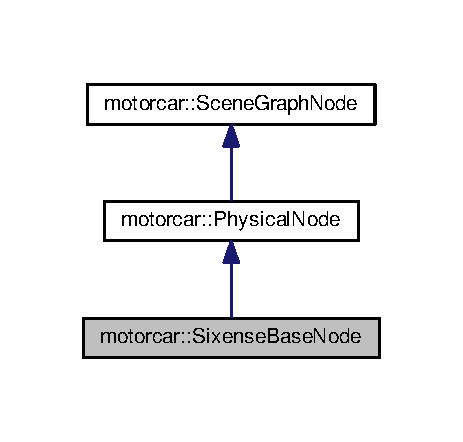
\includegraphics[width=222pt]{classmotorcar_1_1SixenseBaseNode__inherit__graph}
\end{center}
\end{figure}


Collaboration diagram for motorcar\-:\-:Sixense\-Base\-Node\-:
\nopagebreak
\begin{figure}[H]
\begin{center}
\leavevmode
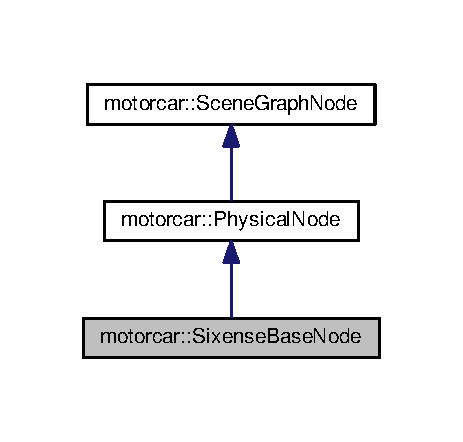
\includegraphics[width=222pt]{classmotorcar_1_1SixenseBaseNode__coll__graph}
\end{center}
\end{figure}
\subsection*{Public Member Functions}
\begin{DoxyCompactItemize}
\item 
\hyperlink{classmotorcar_1_1SixenseBaseNode_a7d0d69617d419cda3837efaa2eaf2d2c}{Sixense\-Base\-Node} (int base\-Index, \hyperlink{classmotorcar_1_1PhysicalNode}{Physical\-Node} $\ast$parent, const glm\-::mat4 \&\hyperlink{classmotorcar_1_1SceneGraphNode_ad96e79fdd739ac8223a3128003be391a}{transform}=glm\-::mat4())
\item 
virtual void \hyperlink{classmotorcar_1_1SixenseBaseNode_a5f211241a5bf54194920582a8bb7e3c3}{handle\-Frame\-Begin} (\hyperlink{classmotorcar_1_1Scene}{Scene} $\ast$\hyperlink{classmotorcar_1_1SceneGraphNode_aa14e637ed4ae98f77e28941a4b5cfdd8}{scene}) override
\begin{DoxyCompactList}\small\item\em gets current system state and passes new controller state to controller nodes \end{DoxyCompactList}\item 
bool \hyperlink{classmotorcar_1_1SixenseBaseNode_a717b0bd837bfaa8a41330ff2e89fe818}{connected} () const 
\item 
void \hyperlink{classmotorcar_1_1SixenseBaseNode_adc93b3ae19192be4d4fbf39bfb5f954b}{set\-Connected} (bool \hyperlink{classmotorcar_1_1SixenseBaseNode_a717b0bd837bfaa8a41330ff2e89fe818}{connected})
\item 
std\-::vector\\*
$<$ \hyperlink{classmotorcar_1_1SixenseControllerNode}{Sixense\-Controller\-Node} $\ast$ $>$ \hyperlink{classmotorcar_1_1SixenseBaseNode_ac15f4bc8939447b77dfeda9749899acc}{controllers} () const 
\end{DoxyCompactItemize}
\subsection*{Additional Inherited Members}


\subsection{Constructor \& Destructor Documentation}
\hypertarget{classmotorcar_1_1SixenseBaseNode_a7d0d69617d419cda3837efaa2eaf2d2c}{\index{motorcar\-::\-Sixense\-Base\-Node@{motorcar\-::\-Sixense\-Base\-Node}!Sixense\-Base\-Node@{Sixense\-Base\-Node}}
\index{Sixense\-Base\-Node@{Sixense\-Base\-Node}!motorcar::SixenseBaseNode@{motorcar\-::\-Sixense\-Base\-Node}}
\subsubsection[{Sixense\-Base\-Node}]{\setlength{\rightskip}{0pt plus 5cm}Sixense\-Base\-Node\-::\-Sixense\-Base\-Node (
\begin{DoxyParamCaption}
\item[{int}]{base\-Index, }
\item[{{\bf Physical\-Node} $\ast$}]{parent, }
\item[{const glm\-::mat4 \&}]{transform = {\ttfamily glm\-:\-:mat4()}}
\end{DoxyParamCaption}
)}}\label{classmotorcar_1_1SixenseBaseNode_a7d0d69617d419cda3837efaa2eaf2d2c}


\subsection{Member Function Documentation}
\hypertarget{classmotorcar_1_1SixenseBaseNode_a717b0bd837bfaa8a41330ff2e89fe818}{\index{motorcar\-::\-Sixense\-Base\-Node@{motorcar\-::\-Sixense\-Base\-Node}!connected@{connected}}
\index{connected@{connected}!motorcar::SixenseBaseNode@{motorcar\-::\-Sixense\-Base\-Node}}
\subsubsection[{connected}]{\setlength{\rightskip}{0pt plus 5cm}bool Sixense\-Base\-Node\-::connected (
\begin{DoxyParamCaption}
{}
\end{DoxyParamCaption}
) const}}\label{classmotorcar_1_1SixenseBaseNode_a717b0bd837bfaa8a41330ff2e89fe818}
\hypertarget{classmotorcar_1_1SixenseBaseNode_ac15f4bc8939447b77dfeda9749899acc}{\index{motorcar\-::\-Sixense\-Base\-Node@{motorcar\-::\-Sixense\-Base\-Node}!controllers@{controllers}}
\index{controllers@{controllers}!motorcar::SixenseBaseNode@{motorcar\-::\-Sixense\-Base\-Node}}
\subsubsection[{controllers}]{\setlength{\rightskip}{0pt plus 5cm}std\-::vector$<$ {\bf Sixense\-Controller\-Node} $\ast$ $>$ Sixense\-Base\-Node\-::controllers (
\begin{DoxyParamCaption}
{}
\end{DoxyParamCaption}
) const}}\label{classmotorcar_1_1SixenseBaseNode_ac15f4bc8939447b77dfeda9749899acc}
\hypertarget{classmotorcar_1_1SixenseBaseNode_a5f211241a5bf54194920582a8bb7e3c3}{\index{motorcar\-::\-Sixense\-Base\-Node@{motorcar\-::\-Sixense\-Base\-Node}!handle\-Frame\-Begin@{handle\-Frame\-Begin}}
\index{handle\-Frame\-Begin@{handle\-Frame\-Begin}!motorcar::SixenseBaseNode@{motorcar\-::\-Sixense\-Base\-Node}}
\subsubsection[{handle\-Frame\-Begin}]{\setlength{\rightskip}{0pt plus 5cm}void Sixense\-Base\-Node\-::handle\-Frame\-Begin (
\begin{DoxyParamCaption}
\item[{{\bf Scene} $\ast$}]{scene}
\end{DoxyParamCaption}
)\hspace{0.3cm}{\ttfamily [override]}, {\ttfamily [virtual]}}}\label{classmotorcar_1_1SixenseBaseNode_a5f211241a5bf54194920582a8bb7e3c3}


gets current system state and passes new controller state to controller nodes 



Reimplemented from \hyperlink{classmotorcar_1_1SceneGraphNode_a494eb20dd66a224888237af89ba6956f}{motorcar\-::\-Scene\-Graph\-Node}.

\hypertarget{classmotorcar_1_1SixenseBaseNode_adc93b3ae19192be4d4fbf39bfb5f954b}{\index{motorcar\-::\-Sixense\-Base\-Node@{motorcar\-::\-Sixense\-Base\-Node}!set\-Connected@{set\-Connected}}
\index{set\-Connected@{set\-Connected}!motorcar::SixenseBaseNode@{motorcar\-::\-Sixense\-Base\-Node}}
\subsubsection[{set\-Connected}]{\setlength{\rightskip}{0pt plus 5cm}void Sixense\-Base\-Node\-::set\-Connected (
\begin{DoxyParamCaption}
\item[{bool}]{connected}
\end{DoxyParamCaption}
)}}\label{classmotorcar_1_1SixenseBaseNode_adc93b3ae19192be4d4fbf39bfb5f954b}


The documentation for this class was generated from the following files\-:\begin{DoxyCompactItemize}
\item 
/home/dave/thesis/motorcar/src/device/\hyperlink{sixensebasenode_8h}{sixensebasenode.\-h}\item 
/home/dave/thesis/motorcar/src/device/\hyperlink{sixensebasenode_8cpp}{sixensebasenode.\-cpp}\end{DoxyCompactItemize}

\hypertarget{classmotorcar_1_1SixenseControllerNode}{\section{motorcar\-:\-:Sixense\-Controller\-Node Class Reference}
\label{classmotorcar_1_1SixenseControllerNode}\index{motorcar\-::\-Sixense\-Controller\-Node@{motorcar\-::\-Sixense\-Controller\-Node}}
}


{\ttfamily \#include $<$sixensecontrollernode.\-h$>$}



Inheritance diagram for motorcar\-:\-:Sixense\-Controller\-Node\-:
\nopagebreak
\begin{figure}[H]
\begin{center}
\leavevmode
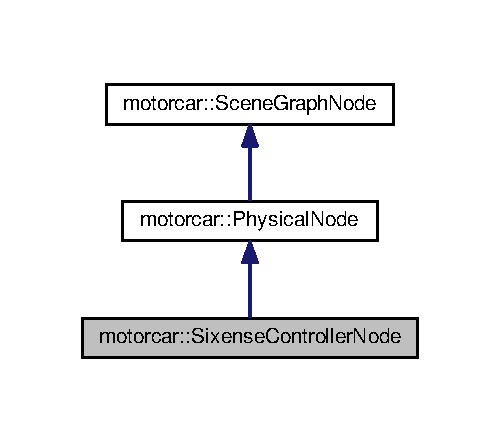
\includegraphics[width=240pt]{classmotorcar_1_1SixenseControllerNode__inherit__graph}
\end{center}
\end{figure}


Collaboration diagram for motorcar\-:\-:Sixense\-Controller\-Node\-:
\nopagebreak
\begin{figure}[H]
\begin{center}
\leavevmode
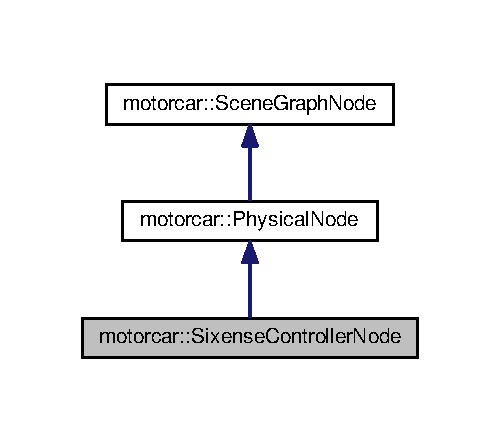
\includegraphics[width=240pt]{classmotorcar_1_1SixenseControllerNode__coll__graph}
\end{center}
\end{figure}
\subsection*{Public Member Functions}
\begin{DoxyCompactItemize}
\item 
\hyperlink{classmotorcar_1_1SixenseControllerNode_acb326fa6a4174d767eedc5563cf8f3bb}{Sixense\-Controller\-Node} (int \hyperlink{classmotorcar_1_1SixenseControllerNode_aa061782ed3ae2a57180fdad9dc6383d9}{controller\-Index}, \hyperlink{classmotorcar_1_1PhysicalNode}{Physical\-Node} $\ast$parent, const glm\-::mat4 \&\hyperlink{classmotorcar_1_1SceneGraphNode_ad96e79fdd739ac8223a3128003be391a}{transform}=glm\-::mat4())
\item 
void \hyperlink{classmotorcar_1_1SixenseControllerNode_afbe76474cf77da7e11b0ac1b291b51f3}{update\-State} (sixense\-Controller\-Data data)
\item 
int \hyperlink{classmotorcar_1_1SixenseControllerNode_aa061782ed3ae2a57180fdad9dc6383d9}{controller\-Index} () const 
\item 
void \hyperlink{classmotorcar_1_1SixenseControllerNode_a337d87a6667b7e35301978c8017f2b20}{set\-Controller\-Index} (int \hyperlink{classmotorcar_1_1SixenseControllerNode_aa061782ed3ae2a57180fdad9dc6383d9}{controller\-Index})
\item 
bool \hyperlink{classmotorcar_1_1SixenseControllerNode_a46ff3af0aa1723d13a7f2a2be599a786}{enabled} () const 
\item 
void \hyperlink{classmotorcar_1_1SixenseControllerNode_aae977f21555500a932f2d9e7a670acd9}{set\-Enabled} (bool \hyperlink{classmotorcar_1_1SixenseControllerNode_a46ff3af0aa1723d13a7f2a2be599a786}{enabled})
\item 
\hyperlink{classmotorcar_1_1SpatialPointingDevice}{Spatial\-Pointing\-Device} $\ast$ \hyperlink{classmotorcar_1_1SixenseControllerNode_ad46bc47d07a912d24d27640f6cea28e4}{pointing\-Device} () const 
\item 
void \hyperlink{classmotorcar_1_1SixenseControllerNode_adab8248c0f5e4adb4a55afca1b096338}{set\-Pointing\-Device} (\hyperlink{classmotorcar_1_1SpatialPointingDevice}{Spatial\-Pointing\-Device} $\ast$\hyperlink{classmotorcar_1_1SixenseControllerNode_ad46bc47d07a912d24d27640f6cea28e4}{pointing\-Device})
\item 
\hyperlink{classmotorcar_1_1SingleBoneTracker}{Single\-Bone\-Tracker} $\ast$ \hyperlink{classmotorcar_1_1SixenseControllerNode_a96ebf0431751aad1153ac0da8845257d}{bone\-Tracker} () const 
\item 
void \hyperlink{classmotorcar_1_1SixenseControllerNode_a99cb44bf2c021c990b9f8bdc46f178f1}{set\-Bone\-Tracker} (\hyperlink{classmotorcar_1_1SingleBoneTracker}{Single\-Bone\-Tracker} $\ast$\hyperlink{classmotorcar_1_1SixenseControllerNode_a96ebf0431751aad1153ac0da8845257d}{bone\-Tracker})
\end{DoxyCompactItemize}
\subsection*{Additional Inherited Members}


\subsection{Constructor \& Destructor Documentation}
\hypertarget{classmotorcar_1_1SixenseControllerNode_acb326fa6a4174d767eedc5563cf8f3bb}{\index{motorcar\-::\-Sixense\-Controller\-Node@{motorcar\-::\-Sixense\-Controller\-Node}!Sixense\-Controller\-Node@{Sixense\-Controller\-Node}}
\index{Sixense\-Controller\-Node@{Sixense\-Controller\-Node}!motorcar::SixenseControllerNode@{motorcar\-::\-Sixense\-Controller\-Node}}
\subsubsection[{Sixense\-Controller\-Node}]{\setlength{\rightskip}{0pt plus 5cm}Sixense\-Controller\-Node\-::\-Sixense\-Controller\-Node (
\begin{DoxyParamCaption}
\item[{int}]{controller\-Index, }
\item[{{\bf Physical\-Node} $\ast$}]{parent, }
\item[{const glm\-::mat4 \&}]{transform = {\ttfamily glm\-:\-:mat4()}}
\end{DoxyParamCaption}
)}}\label{classmotorcar_1_1SixenseControllerNode_acb326fa6a4174d767eedc5563cf8f3bb}


\subsection{Member Function Documentation}
\hypertarget{classmotorcar_1_1SixenseControllerNode_a96ebf0431751aad1153ac0da8845257d}{\index{motorcar\-::\-Sixense\-Controller\-Node@{motorcar\-::\-Sixense\-Controller\-Node}!bone\-Tracker@{bone\-Tracker}}
\index{bone\-Tracker@{bone\-Tracker}!motorcar::SixenseControllerNode@{motorcar\-::\-Sixense\-Controller\-Node}}
\subsubsection[{bone\-Tracker}]{\setlength{\rightskip}{0pt plus 5cm}{\bf Single\-Bone\-Tracker} $\ast$ Sixense\-Controller\-Node\-::bone\-Tracker (
\begin{DoxyParamCaption}
{}
\end{DoxyParamCaption}
) const}}\label{classmotorcar_1_1SixenseControllerNode_a96ebf0431751aad1153ac0da8845257d}
\hypertarget{classmotorcar_1_1SixenseControllerNode_aa061782ed3ae2a57180fdad9dc6383d9}{\index{motorcar\-::\-Sixense\-Controller\-Node@{motorcar\-::\-Sixense\-Controller\-Node}!controller\-Index@{controller\-Index}}
\index{controller\-Index@{controller\-Index}!motorcar::SixenseControllerNode@{motorcar\-::\-Sixense\-Controller\-Node}}
\subsubsection[{controller\-Index}]{\setlength{\rightskip}{0pt plus 5cm}int Sixense\-Controller\-Node\-::controller\-Index (
\begin{DoxyParamCaption}
{}
\end{DoxyParamCaption}
) const}}\label{classmotorcar_1_1SixenseControllerNode_aa061782ed3ae2a57180fdad9dc6383d9}
\hypertarget{classmotorcar_1_1SixenseControllerNode_a46ff3af0aa1723d13a7f2a2be599a786}{\index{motorcar\-::\-Sixense\-Controller\-Node@{motorcar\-::\-Sixense\-Controller\-Node}!enabled@{enabled}}
\index{enabled@{enabled}!motorcar::SixenseControllerNode@{motorcar\-::\-Sixense\-Controller\-Node}}
\subsubsection[{enabled}]{\setlength{\rightskip}{0pt plus 5cm}bool Sixense\-Controller\-Node\-::enabled (
\begin{DoxyParamCaption}
{}
\end{DoxyParamCaption}
) const}}\label{classmotorcar_1_1SixenseControllerNode_a46ff3af0aa1723d13a7f2a2be599a786}
\hypertarget{classmotorcar_1_1SixenseControllerNode_ad46bc47d07a912d24d27640f6cea28e4}{\index{motorcar\-::\-Sixense\-Controller\-Node@{motorcar\-::\-Sixense\-Controller\-Node}!pointing\-Device@{pointing\-Device}}
\index{pointing\-Device@{pointing\-Device}!motorcar::SixenseControllerNode@{motorcar\-::\-Sixense\-Controller\-Node}}
\subsubsection[{pointing\-Device}]{\setlength{\rightskip}{0pt plus 5cm}{\bf Spatial\-Pointing\-Device} $\ast$ Sixense\-Controller\-Node\-::pointing\-Device (
\begin{DoxyParamCaption}
{}
\end{DoxyParamCaption}
) const}}\label{classmotorcar_1_1SixenseControllerNode_ad46bc47d07a912d24d27640f6cea28e4}
\hypertarget{classmotorcar_1_1SixenseControllerNode_a99cb44bf2c021c990b9f8bdc46f178f1}{\index{motorcar\-::\-Sixense\-Controller\-Node@{motorcar\-::\-Sixense\-Controller\-Node}!set\-Bone\-Tracker@{set\-Bone\-Tracker}}
\index{set\-Bone\-Tracker@{set\-Bone\-Tracker}!motorcar::SixenseControllerNode@{motorcar\-::\-Sixense\-Controller\-Node}}
\subsubsection[{set\-Bone\-Tracker}]{\setlength{\rightskip}{0pt plus 5cm}void Sixense\-Controller\-Node\-::set\-Bone\-Tracker (
\begin{DoxyParamCaption}
\item[{{\bf Single\-Bone\-Tracker} $\ast$}]{bone\-Tracker}
\end{DoxyParamCaption}
)}}\label{classmotorcar_1_1SixenseControllerNode_a99cb44bf2c021c990b9f8bdc46f178f1}
\hypertarget{classmotorcar_1_1SixenseControllerNode_a337d87a6667b7e35301978c8017f2b20}{\index{motorcar\-::\-Sixense\-Controller\-Node@{motorcar\-::\-Sixense\-Controller\-Node}!set\-Controller\-Index@{set\-Controller\-Index}}
\index{set\-Controller\-Index@{set\-Controller\-Index}!motorcar::SixenseControllerNode@{motorcar\-::\-Sixense\-Controller\-Node}}
\subsubsection[{set\-Controller\-Index}]{\setlength{\rightskip}{0pt plus 5cm}void Sixense\-Controller\-Node\-::set\-Controller\-Index (
\begin{DoxyParamCaption}
\item[{int}]{controller\-Index}
\end{DoxyParamCaption}
)}}\label{classmotorcar_1_1SixenseControllerNode_a337d87a6667b7e35301978c8017f2b20}
\hypertarget{classmotorcar_1_1SixenseControllerNode_aae977f21555500a932f2d9e7a670acd9}{\index{motorcar\-::\-Sixense\-Controller\-Node@{motorcar\-::\-Sixense\-Controller\-Node}!set\-Enabled@{set\-Enabled}}
\index{set\-Enabled@{set\-Enabled}!motorcar::SixenseControllerNode@{motorcar\-::\-Sixense\-Controller\-Node}}
\subsubsection[{set\-Enabled}]{\setlength{\rightskip}{0pt plus 5cm}void Sixense\-Controller\-Node\-::set\-Enabled (
\begin{DoxyParamCaption}
\item[{bool}]{enabled}
\end{DoxyParamCaption}
)}}\label{classmotorcar_1_1SixenseControllerNode_aae977f21555500a932f2d9e7a670acd9}
\hypertarget{classmotorcar_1_1SixenseControllerNode_adab8248c0f5e4adb4a55afca1b096338}{\index{motorcar\-::\-Sixense\-Controller\-Node@{motorcar\-::\-Sixense\-Controller\-Node}!set\-Pointing\-Device@{set\-Pointing\-Device}}
\index{set\-Pointing\-Device@{set\-Pointing\-Device}!motorcar::SixenseControllerNode@{motorcar\-::\-Sixense\-Controller\-Node}}
\subsubsection[{set\-Pointing\-Device}]{\setlength{\rightskip}{0pt plus 5cm}void Sixense\-Controller\-Node\-::set\-Pointing\-Device (
\begin{DoxyParamCaption}
\item[{{\bf Spatial\-Pointing\-Device} $\ast$}]{pointing\-Device}
\end{DoxyParamCaption}
)}}\label{classmotorcar_1_1SixenseControllerNode_adab8248c0f5e4adb4a55afca1b096338}
\hypertarget{classmotorcar_1_1SixenseControllerNode_afbe76474cf77da7e11b0ac1b291b51f3}{\index{motorcar\-::\-Sixense\-Controller\-Node@{motorcar\-::\-Sixense\-Controller\-Node}!update\-State@{update\-State}}
\index{update\-State@{update\-State}!motorcar::SixenseControllerNode@{motorcar\-::\-Sixense\-Controller\-Node}}
\subsubsection[{update\-State}]{\setlength{\rightskip}{0pt plus 5cm}void Sixense\-Controller\-Node\-::update\-State (
\begin{DoxyParamCaption}
\item[{sixense\-Controller\-Data}]{data}
\end{DoxyParamCaption}
)}}\label{classmotorcar_1_1SixenseControllerNode_afbe76474cf77da7e11b0ac1b291b51f3}


The documentation for this class was generated from the following files\-:\begin{DoxyCompactItemize}
\item 
/media/dave/e89b5eb4-\/4b10-\/4edf-\/8ad5-\/0d046a46b978/dave/thesis/qtwayland-\/motorcar-\/compositor/motorcar/src/device/\hyperlink{sixensecontrollernode_8h}{sixensecontrollernode.\-h}\item 
/media/dave/e89b5eb4-\/4b10-\/4edf-\/8ad5-\/0d046a46b978/dave/thesis/qtwayland-\/motorcar-\/compositor/motorcar/src/device/\hyperlink{sixensecontrollernode_8cpp}{sixensecontrollernode.\-cpp}\end{DoxyCompactItemize}

\hypertarget{classmotorcar_1_1SixenseMotionSensingSystem}{\section{motorcar\-:\-:Sixense\-Motion\-Sensing\-System Class Reference}
\label{classmotorcar_1_1SixenseMotionSensingSystem}\index{motorcar\-::\-Sixense\-Motion\-Sensing\-System@{motorcar\-::\-Sixense\-Motion\-Sensing\-System}}
}


{\ttfamily \#include $<$sixensemotionsensingsystem.\-h$>$}

\subsection*{Public Member Functions}
\begin{DoxyCompactItemize}
\item 
\hyperlink{classmotorcar_1_1SixenseMotionSensingSystem_a36e5d5612aabed32df976c19cfacec2d}{Sixense\-Motion\-Sensing\-System} (\hyperlink{classmotorcar_1_1Scene}{Scene} $\ast$scene)
\item 
\hyperlink{classmotorcar_1_1SixenseMotionSensingSystem_aa9d2334b2f0e2912e719e538a051f952}{$\sim$\-Sixense\-Motion\-Sensing\-System} ()
\item 
bool \hyperlink{classmotorcar_1_1SixenseMotionSensingSystem_ac58c619e72581bc1d268851f4349c07a}{is\-Initialized} () const 
\item 
std\-::vector$<$ \hyperlink{classmotorcar_1_1SixenseBaseNode}{Sixense\-Base\-Node} $\ast$ $>$ \hyperlink{classmotorcar_1_1SixenseMotionSensingSystem_ac5ed9086cca91cd68b4b038505419bd2}{base\-Stations} () const 
\end{DoxyCompactItemize}
\subsection*{Static Public Member Functions}
\begin{DoxyCompactItemize}
\item 
static void \hyperlink{classmotorcar_1_1SixenseMotionSensingSystem_a6ba2385c755b3e922d3272c9ddeb70dd}{controller\-Manager\-Setup\-Callback} (sixense\-Utils\-::\-Controller\-Manager\-::setup\-\_\-step step)
\end{DoxyCompactItemize}


\subsection{Constructor \& Destructor Documentation}
\hypertarget{classmotorcar_1_1SixenseMotionSensingSystem_a36e5d5612aabed32df976c19cfacec2d}{\index{motorcar\-::\-Sixense\-Motion\-Sensing\-System@{motorcar\-::\-Sixense\-Motion\-Sensing\-System}!Sixense\-Motion\-Sensing\-System@{Sixense\-Motion\-Sensing\-System}}
\index{Sixense\-Motion\-Sensing\-System@{Sixense\-Motion\-Sensing\-System}!motorcar::SixenseMotionSensingSystem@{motorcar\-::\-Sixense\-Motion\-Sensing\-System}}
\subsubsection[{Sixense\-Motion\-Sensing\-System}]{\setlength{\rightskip}{0pt plus 5cm}Sixense\-Motion\-Sensing\-System\-::\-Sixense\-Motion\-Sensing\-System (
\begin{DoxyParamCaption}
\item[{{\bf Scene} $\ast$}]{scene}
\end{DoxyParamCaption}
)}}\label{classmotorcar_1_1SixenseMotionSensingSystem_a36e5d5612aabed32df976c19cfacec2d}
\hypertarget{classmotorcar_1_1SixenseMotionSensingSystem_aa9d2334b2f0e2912e719e538a051f952}{\index{motorcar\-::\-Sixense\-Motion\-Sensing\-System@{motorcar\-::\-Sixense\-Motion\-Sensing\-System}!$\sim$\-Sixense\-Motion\-Sensing\-System@{$\sim$\-Sixense\-Motion\-Sensing\-System}}
\index{$\sim$\-Sixense\-Motion\-Sensing\-System@{$\sim$\-Sixense\-Motion\-Sensing\-System}!motorcar::SixenseMotionSensingSystem@{motorcar\-::\-Sixense\-Motion\-Sensing\-System}}
\subsubsection[{$\sim$\-Sixense\-Motion\-Sensing\-System}]{\setlength{\rightskip}{0pt plus 5cm}Sixense\-Motion\-Sensing\-System\-::$\sim$\-Sixense\-Motion\-Sensing\-System (
\begin{DoxyParamCaption}
{}
\end{DoxyParamCaption}
)}}\label{classmotorcar_1_1SixenseMotionSensingSystem_aa9d2334b2f0e2912e719e538a051f952}


\subsection{Member Function Documentation}
\hypertarget{classmotorcar_1_1SixenseMotionSensingSystem_ac5ed9086cca91cd68b4b038505419bd2}{\index{motorcar\-::\-Sixense\-Motion\-Sensing\-System@{motorcar\-::\-Sixense\-Motion\-Sensing\-System}!base\-Stations@{base\-Stations}}
\index{base\-Stations@{base\-Stations}!motorcar::SixenseMotionSensingSystem@{motorcar\-::\-Sixense\-Motion\-Sensing\-System}}
\subsubsection[{base\-Stations}]{\setlength{\rightskip}{0pt plus 5cm}std\-::vector$<$ {\bf Sixense\-Base\-Node} $\ast$ $>$ Sixense\-Motion\-Sensing\-System\-::base\-Stations (
\begin{DoxyParamCaption}
{}
\end{DoxyParamCaption}
) const}}\label{classmotorcar_1_1SixenseMotionSensingSystem_ac5ed9086cca91cd68b4b038505419bd2}
\hypertarget{classmotorcar_1_1SixenseMotionSensingSystem_a6ba2385c755b3e922d3272c9ddeb70dd}{\index{motorcar\-::\-Sixense\-Motion\-Sensing\-System@{motorcar\-::\-Sixense\-Motion\-Sensing\-System}!controller\-Manager\-Setup\-Callback@{controller\-Manager\-Setup\-Callback}}
\index{controller\-Manager\-Setup\-Callback@{controller\-Manager\-Setup\-Callback}!motorcar::SixenseMotionSensingSystem@{motorcar\-::\-Sixense\-Motion\-Sensing\-System}}
\subsubsection[{controller\-Manager\-Setup\-Callback}]{\setlength{\rightskip}{0pt plus 5cm}void Sixense\-Motion\-Sensing\-System\-::controller\-Manager\-Setup\-Callback (
\begin{DoxyParamCaption}
\item[{sixense\-Utils\-::\-Controller\-Manager\-::setup\-\_\-step}]{step}
\end{DoxyParamCaption}
)\hspace{0.3cm}{\ttfamily [static]}}}\label{classmotorcar_1_1SixenseMotionSensingSystem_a6ba2385c755b3e922d3272c9ddeb70dd}
\hypertarget{classmotorcar_1_1SixenseMotionSensingSystem_ac58c619e72581bc1d268851f4349c07a}{\index{motorcar\-::\-Sixense\-Motion\-Sensing\-System@{motorcar\-::\-Sixense\-Motion\-Sensing\-System}!is\-Initialized@{is\-Initialized}}
\index{is\-Initialized@{is\-Initialized}!motorcar::SixenseMotionSensingSystem@{motorcar\-::\-Sixense\-Motion\-Sensing\-System}}
\subsubsection[{is\-Initialized}]{\setlength{\rightskip}{0pt plus 5cm}bool Sixense\-Motion\-Sensing\-System\-::is\-Initialized (
\begin{DoxyParamCaption}
{}
\end{DoxyParamCaption}
) const}}\label{classmotorcar_1_1SixenseMotionSensingSystem_ac58c619e72581bc1d268851f4349c07a}


The documentation for this class was generated from the following files\-:\begin{DoxyCompactItemize}
\item 
/home/dave/thesis/motorcar/src/device/\hyperlink{sixensemotionsensingsystem_8h}{sixensemotionsensingsystem.\-h}\item 
/home/dave/thesis/motorcar/src/device/\hyperlink{sixensemotionsensingsystem_8cpp}{sixensemotionsensingsystem.\-cpp}\end{DoxyCompactItemize}

\hypertarget{classmotorcar_1_1SpatialPointingDevice}{\section{motorcar\-:\-:Spatial\-Pointing\-Device Class Reference}
\label{classmotorcar_1_1SpatialPointingDevice}\index{motorcar\-::\-Spatial\-Pointing\-Device@{motorcar\-::\-Spatial\-Pointing\-Device}}
}


{\ttfamily \#include $<$spatialpointingdevice.\-h$>$}



Inheritance diagram for motorcar\-:\-:Spatial\-Pointing\-Device\-:
\nopagebreak
\begin{figure}[H]
\begin{center}
\leavevmode
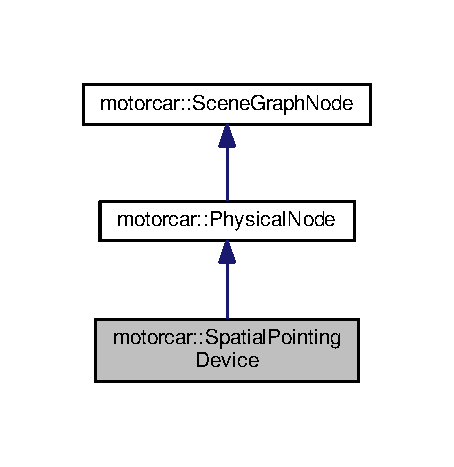
\includegraphics[height=550pt]{classmotorcar_1_1SpatialPointingDevice__inherit__graph}
\end{center}
\end{figure}


Collaboration diagram for motorcar\-:\-:Spatial\-Pointing\-Device\-:
\nopagebreak
\begin{figure}[H]
\begin{center}
\leavevmode
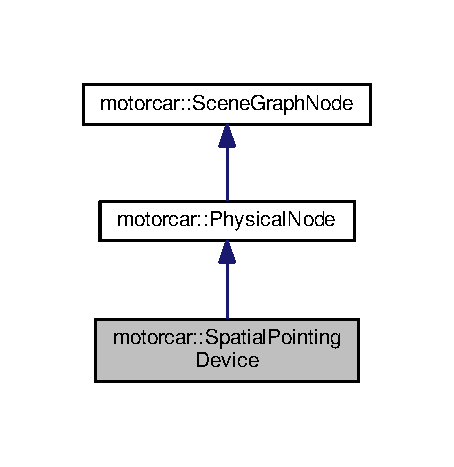
\includegraphics[height=550pt]{classmotorcar_1_1SpatialPointingDevice__coll__graph}
\end{center}
\end{figure}
\subsection*{Public Member Functions}
\begin{DoxyCompactItemize}
\item 
\hyperlink{classmotorcar_1_1SpatialPointingDevice_a5e6ae01142cf0324623fd8481ad949ea}{Spatial\-Pointing\-Device} (\hyperlink{classmotorcar_1_1PhysicalNode}{Physical\-Node} $\ast$parent, const glm\-::mat4 \&\hyperlink{classmotorcar_1_1SceneGraphNode_ad96e79fdd739ac8223a3128003be391a}{transform}=glm\-::mat4())
\item 
virtual \hyperlink{classmotorcar_1_1SpatialPointingDevice_a2232e5d48af72563948b3dcf87467ba4}{$\sim$\-Spatial\-Pointing\-Device} ()
\item 
void \hyperlink{classmotorcar_1_1SpatialPointingDevice_a53e251f5a0d7a9b0b8e7dc84d2e9d078}{traverse\-Node} (\hyperlink{classmotorcar_1_1Scene}{Scene} $\ast$\hyperlink{classmotorcar_1_1SceneGraphNode_aa14e637ed4ae98f77e28941a4b5cfdd8}{scene}, long delta\-Millis) override
\item 
bool \hyperlink{classmotorcar_1_1SpatialPointingDevice_a00473664d02c3adc6636515d328115d8}{left\-Mouse\-Down} () const 
\item 
void \hyperlink{classmotorcar_1_1SpatialPointingDevice_a8d5fb9adf62c0c808c9c08369206d47a}{set\-Left\-Mouse\-Down} (bool \hyperlink{classmotorcar_1_1SpatialPointingDevice_a00473664d02c3adc6636515d328115d8}{left\-Mouse\-Down})
\item 
bool \hyperlink{classmotorcar_1_1SpatialPointingDevice_ae419894256240b9815dd88675be03f00}{right\-Mouse\-Down} () const 
\item 
void \hyperlink{classmotorcar_1_1SpatialPointingDevice_a260a837c910d3e640df05b63b44c052e}{set\-Right\-Mouse\-Down} (bool \hyperlink{classmotorcar_1_1SpatialPointingDevice_ae419894256240b9815dd88675be03f00}{right\-Mouse\-Down})
\item 
bool \hyperlink{classmotorcar_1_1SpatialPointingDevice_aa41dd8386cb72b3813f54af4175f8bd3}{middle\-Mouse\-Down} () const 
\item 
void \hyperlink{classmotorcar_1_1SpatialPointingDevice_ac582041efeac1940a72ddc33e352101e}{set\-Middle\-Mouse\-Down} (bool \hyperlink{classmotorcar_1_1SpatialPointingDevice_aa41dd8386cb72b3813f54af4175f8bd3}{middle\-Mouse\-Down})
\item 
void \hyperlink{classmotorcar_1_1SpatialPointingDevice_ab34f8c2ab699085b5f1d78aecd961614}{grab\-Surface\-Under\-Cursor} ()
\item 
void \hyperlink{classmotorcar_1_1SpatialPointingDevice_a53cd4de170f2f69d95c9d3ee38876060}{release\-Grabbed\-Surface} ()
\end{DoxyCompactItemize}
\subsection*{Additional Inherited Members}


\subsection{Constructor \& Destructor Documentation}
\hypertarget{classmotorcar_1_1SpatialPointingDevice_a5e6ae01142cf0324623fd8481ad949ea}{\index{motorcar\-::\-Spatial\-Pointing\-Device@{motorcar\-::\-Spatial\-Pointing\-Device}!Spatial\-Pointing\-Device@{Spatial\-Pointing\-Device}}
\index{Spatial\-Pointing\-Device@{Spatial\-Pointing\-Device}!motorcar::SpatialPointingDevice@{motorcar\-::\-Spatial\-Pointing\-Device}}
\subsubsection[{Spatial\-Pointing\-Device}]{\setlength{\rightskip}{0pt plus 5cm}Spatial\-Pointing\-Device\-::\-Spatial\-Pointing\-Device (
\begin{DoxyParamCaption}
\item[{{\bf Physical\-Node} $\ast$}]{parent, }
\item[{const glm\-::mat4 \&}]{transform = {\ttfamily glm\-:\-:mat4()}}
\end{DoxyParamCaption}
)}}\label{classmotorcar_1_1SpatialPointingDevice_a5e6ae01142cf0324623fd8481ad949ea}
\hypertarget{classmotorcar_1_1SpatialPointingDevice_a2232e5d48af72563948b3dcf87467ba4}{\index{motorcar\-::\-Spatial\-Pointing\-Device@{motorcar\-::\-Spatial\-Pointing\-Device}!$\sim$\-Spatial\-Pointing\-Device@{$\sim$\-Spatial\-Pointing\-Device}}
\index{$\sim$\-Spatial\-Pointing\-Device@{$\sim$\-Spatial\-Pointing\-Device}!motorcar::SpatialPointingDevice@{motorcar\-::\-Spatial\-Pointing\-Device}}
\subsubsection[{$\sim$\-Spatial\-Pointing\-Device}]{\setlength{\rightskip}{0pt plus 5cm}virtual motorcar\-::\-Spatial\-Pointing\-Device\-::$\sim$\-Spatial\-Pointing\-Device (
\begin{DoxyParamCaption}
{}
\end{DoxyParamCaption}
)\hspace{0.3cm}{\ttfamily [inline]}, {\ttfamily [virtual]}}}\label{classmotorcar_1_1SpatialPointingDevice_a2232e5d48af72563948b3dcf87467ba4}


\subsection{Member Function Documentation}
\hypertarget{classmotorcar_1_1SpatialPointingDevice_ab34f8c2ab699085b5f1d78aecd961614}{\index{motorcar\-::\-Spatial\-Pointing\-Device@{motorcar\-::\-Spatial\-Pointing\-Device}!grab\-Surface\-Under\-Cursor@{grab\-Surface\-Under\-Cursor}}
\index{grab\-Surface\-Under\-Cursor@{grab\-Surface\-Under\-Cursor}!motorcar::SpatialPointingDevice@{motorcar\-::\-Spatial\-Pointing\-Device}}
\subsubsection[{grab\-Surface\-Under\-Cursor}]{\setlength{\rightskip}{0pt plus 5cm}void Spatial\-Pointing\-Device\-::grab\-Surface\-Under\-Cursor (
\begin{DoxyParamCaption}
{}
\end{DoxyParamCaption}
)}}\label{classmotorcar_1_1SpatialPointingDevice_ab34f8c2ab699085b5f1d78aecd961614}
\hypertarget{classmotorcar_1_1SpatialPointingDevice_a00473664d02c3adc6636515d328115d8}{\index{motorcar\-::\-Spatial\-Pointing\-Device@{motorcar\-::\-Spatial\-Pointing\-Device}!left\-Mouse\-Down@{left\-Mouse\-Down}}
\index{left\-Mouse\-Down@{left\-Mouse\-Down}!motorcar::SpatialPointingDevice@{motorcar\-::\-Spatial\-Pointing\-Device}}
\subsubsection[{left\-Mouse\-Down}]{\setlength{\rightskip}{0pt plus 5cm}bool Spatial\-Pointing\-Device\-::left\-Mouse\-Down (
\begin{DoxyParamCaption}
{}
\end{DoxyParamCaption}
) const}}\label{classmotorcar_1_1SpatialPointingDevice_a00473664d02c3adc6636515d328115d8}
\hypertarget{classmotorcar_1_1SpatialPointingDevice_aa41dd8386cb72b3813f54af4175f8bd3}{\index{motorcar\-::\-Spatial\-Pointing\-Device@{motorcar\-::\-Spatial\-Pointing\-Device}!middle\-Mouse\-Down@{middle\-Mouse\-Down}}
\index{middle\-Mouse\-Down@{middle\-Mouse\-Down}!motorcar::SpatialPointingDevice@{motorcar\-::\-Spatial\-Pointing\-Device}}
\subsubsection[{middle\-Mouse\-Down}]{\setlength{\rightskip}{0pt plus 5cm}bool Spatial\-Pointing\-Device\-::middle\-Mouse\-Down (
\begin{DoxyParamCaption}
{}
\end{DoxyParamCaption}
) const}}\label{classmotorcar_1_1SpatialPointingDevice_aa41dd8386cb72b3813f54af4175f8bd3}
\hypertarget{classmotorcar_1_1SpatialPointingDevice_a53cd4de170f2f69d95c9d3ee38876060}{\index{motorcar\-::\-Spatial\-Pointing\-Device@{motorcar\-::\-Spatial\-Pointing\-Device}!release\-Grabbed\-Surface@{release\-Grabbed\-Surface}}
\index{release\-Grabbed\-Surface@{release\-Grabbed\-Surface}!motorcar::SpatialPointingDevice@{motorcar\-::\-Spatial\-Pointing\-Device}}
\subsubsection[{release\-Grabbed\-Surface}]{\setlength{\rightskip}{0pt plus 5cm}void Spatial\-Pointing\-Device\-::release\-Grabbed\-Surface (
\begin{DoxyParamCaption}
{}
\end{DoxyParamCaption}
)}}\label{classmotorcar_1_1SpatialPointingDevice_a53cd4de170f2f69d95c9d3ee38876060}
\hypertarget{classmotorcar_1_1SpatialPointingDevice_ae419894256240b9815dd88675be03f00}{\index{motorcar\-::\-Spatial\-Pointing\-Device@{motorcar\-::\-Spatial\-Pointing\-Device}!right\-Mouse\-Down@{right\-Mouse\-Down}}
\index{right\-Mouse\-Down@{right\-Mouse\-Down}!motorcar::SpatialPointingDevice@{motorcar\-::\-Spatial\-Pointing\-Device}}
\subsubsection[{right\-Mouse\-Down}]{\setlength{\rightskip}{0pt plus 5cm}bool Spatial\-Pointing\-Device\-::right\-Mouse\-Down (
\begin{DoxyParamCaption}
{}
\end{DoxyParamCaption}
) const}}\label{classmotorcar_1_1SpatialPointingDevice_ae419894256240b9815dd88675be03f00}
\hypertarget{classmotorcar_1_1SpatialPointingDevice_a8d5fb9adf62c0c808c9c08369206d47a}{\index{motorcar\-::\-Spatial\-Pointing\-Device@{motorcar\-::\-Spatial\-Pointing\-Device}!set\-Left\-Mouse\-Down@{set\-Left\-Mouse\-Down}}
\index{set\-Left\-Mouse\-Down@{set\-Left\-Mouse\-Down}!motorcar::SpatialPointingDevice@{motorcar\-::\-Spatial\-Pointing\-Device}}
\subsubsection[{set\-Left\-Mouse\-Down}]{\setlength{\rightskip}{0pt plus 5cm}void Spatial\-Pointing\-Device\-::set\-Left\-Mouse\-Down (
\begin{DoxyParamCaption}
\item[{bool}]{left\-Mouse\-Down}
\end{DoxyParamCaption}
)}}\label{classmotorcar_1_1SpatialPointingDevice_a8d5fb9adf62c0c808c9c08369206d47a}
\hypertarget{classmotorcar_1_1SpatialPointingDevice_ac582041efeac1940a72ddc33e352101e}{\index{motorcar\-::\-Spatial\-Pointing\-Device@{motorcar\-::\-Spatial\-Pointing\-Device}!set\-Middle\-Mouse\-Down@{set\-Middle\-Mouse\-Down}}
\index{set\-Middle\-Mouse\-Down@{set\-Middle\-Mouse\-Down}!motorcar::SpatialPointingDevice@{motorcar\-::\-Spatial\-Pointing\-Device}}
\subsubsection[{set\-Middle\-Mouse\-Down}]{\setlength{\rightskip}{0pt plus 5cm}void Spatial\-Pointing\-Device\-::set\-Middle\-Mouse\-Down (
\begin{DoxyParamCaption}
\item[{bool}]{middle\-Mouse\-Down}
\end{DoxyParamCaption}
)}}\label{classmotorcar_1_1SpatialPointingDevice_ac582041efeac1940a72ddc33e352101e}
\hypertarget{classmotorcar_1_1SpatialPointingDevice_a260a837c910d3e640df05b63b44c052e}{\index{motorcar\-::\-Spatial\-Pointing\-Device@{motorcar\-::\-Spatial\-Pointing\-Device}!set\-Right\-Mouse\-Down@{set\-Right\-Mouse\-Down}}
\index{set\-Right\-Mouse\-Down@{set\-Right\-Mouse\-Down}!motorcar::SpatialPointingDevice@{motorcar\-::\-Spatial\-Pointing\-Device}}
\subsubsection[{set\-Right\-Mouse\-Down}]{\setlength{\rightskip}{0pt plus 5cm}void Spatial\-Pointing\-Device\-::set\-Right\-Mouse\-Down (
\begin{DoxyParamCaption}
\item[{bool}]{right\-Mouse\-Down}
\end{DoxyParamCaption}
)}}\label{classmotorcar_1_1SpatialPointingDevice_a260a837c910d3e640df05b63b44c052e}
\hypertarget{classmotorcar_1_1SpatialPointingDevice_a53e251f5a0d7a9b0b8e7dc84d2e9d078}{\index{motorcar\-::\-Spatial\-Pointing\-Device@{motorcar\-::\-Spatial\-Pointing\-Device}!traverse\-Node@{traverse\-Node}}
\index{traverse\-Node@{traverse\-Node}!motorcar::SpatialPointingDevice@{motorcar\-::\-Spatial\-Pointing\-Device}}
\subsubsection[{traverse\-Node}]{\setlength{\rightskip}{0pt plus 5cm}void Spatial\-Pointing\-Device\-::traverse\-Node (
\begin{DoxyParamCaption}
\item[{{\bf Scene} $\ast$}]{scene, }
\item[{long}]{delta\-Millis}
\end{DoxyParamCaption}
)\hspace{0.3cm}{\ttfamily [override]}, {\ttfamily [virtual]}}}\label{classmotorcar_1_1SpatialPointingDevice_a53e251f5a0d7a9b0b8e7dc84d2e9d078}


Reimplemented from \hyperlink{classmotorcar_1_1SceneGraphNode_aa680a8e89fc8ebd12b784653fb30c29a}{motorcar\-::\-Scene\-Graph\-Node}.



The documentation for this class was generated from the following files\-:\begin{DoxyCompactItemize}
\item 
/home/dave/thesis/qtwayland-\/motorcar-\/compositor/motorcar/src/scenegraph/input/\hyperlink{spatialpointingdevice_8h}{spatialpointingdevice.\-h}\item 
/home/dave/thesis/qtwayland-\/motorcar-\/compositor/motorcar/src/scenegraph/input/\hyperlink{spatialpointingdevice_8cpp}{spatialpointingdevice.\-cpp}\end{DoxyCompactItemize}

\hypertarget{classTextureBlitter}{\section{Texture\-Blitter Class Reference}
\label{classTextureBlitter}\index{Texture\-Blitter@{Texture\-Blitter}}
}


{\ttfamily \#include $<$textureblitter.\-h$>$}

\subsection*{Public Member Functions}
\begin{DoxyCompactItemize}
\item 
\hyperlink{classTextureBlitter_a4e6e3fad09aa0fe61d86ef9e540b7624}{Texture\-Blitter} ()
\item 
\hyperlink{classTextureBlitter_a1af0b8757619a773db318647a953b6b3}{$\sim$\-Texture\-Blitter} ()
\item 
void \hyperlink{classTextureBlitter_aa71be8ffe16fc0161fa8a4cc89e4656d}{bind} ()
\item 
void \hyperlink{classTextureBlitter_acd6756b8a64f87fcdd8aa09ab9a366a7}{release} ()
\item 
void \hyperlink{classTextureBlitter_a0cf7d65fbe8eeefa4d690d60471750d2}{draw\-Texture} (int texture\-Id, const Q\-Rect\-F \&source\-Geometry, const Q\-Size \&target\-Rect, int depth, bool targethas\-Inverted\-Y, bool source\-Has\-Inverted\-Y)
\end{DoxyCompactItemize}


\subsection{Constructor \& Destructor Documentation}
\hypertarget{classTextureBlitter_a4e6e3fad09aa0fe61d86ef9e540b7624}{\index{Texture\-Blitter@{Texture\-Blitter}!Texture\-Blitter@{Texture\-Blitter}}
\index{Texture\-Blitter@{Texture\-Blitter}!TextureBlitter@{Texture\-Blitter}}
\subsubsection[{Texture\-Blitter}]{\setlength{\rightskip}{0pt plus 5cm}Texture\-Blitter\-::\-Texture\-Blitter (
\begin{DoxyParamCaption}
{}
\end{DoxyParamCaption}
)}}\label{classTextureBlitter_a4e6e3fad09aa0fe61d86ef9e540b7624}
\hypertarget{classTextureBlitter_a1af0b8757619a773db318647a953b6b3}{\index{Texture\-Blitter@{Texture\-Blitter}!$\sim$\-Texture\-Blitter@{$\sim$\-Texture\-Blitter}}
\index{$\sim$\-Texture\-Blitter@{$\sim$\-Texture\-Blitter}!TextureBlitter@{Texture\-Blitter}}
\subsubsection[{$\sim$\-Texture\-Blitter}]{\setlength{\rightskip}{0pt plus 5cm}Texture\-Blitter\-::$\sim$\-Texture\-Blitter (
\begin{DoxyParamCaption}
{}
\end{DoxyParamCaption}
)}}\label{classTextureBlitter_a1af0b8757619a773db318647a953b6b3}


\subsection{Member Function Documentation}
\hypertarget{classTextureBlitter_aa71be8ffe16fc0161fa8a4cc89e4656d}{\index{Texture\-Blitter@{Texture\-Blitter}!bind@{bind}}
\index{bind@{bind}!TextureBlitter@{Texture\-Blitter}}
\subsubsection[{bind}]{\setlength{\rightskip}{0pt plus 5cm}void Texture\-Blitter\-::bind (
\begin{DoxyParamCaption}
{}
\end{DoxyParamCaption}
)}}\label{classTextureBlitter_aa71be8ffe16fc0161fa8a4cc89e4656d}
\hypertarget{classTextureBlitter_a0cf7d65fbe8eeefa4d690d60471750d2}{\index{Texture\-Blitter@{Texture\-Blitter}!draw\-Texture@{draw\-Texture}}
\index{draw\-Texture@{draw\-Texture}!TextureBlitter@{Texture\-Blitter}}
\subsubsection[{draw\-Texture}]{\setlength{\rightskip}{0pt plus 5cm}void Texture\-Blitter\-::draw\-Texture (
\begin{DoxyParamCaption}
\item[{int}]{texture\-Id, }
\item[{const Q\-Rect\-F \&}]{source\-Geometry, }
\item[{const Q\-Size \&}]{target\-Rect, }
\item[{int}]{depth, }
\item[{bool}]{targethas\-Inverted\-Y, }
\item[{bool}]{source\-Has\-Inverted\-Y}
\end{DoxyParamCaption}
)}}\label{classTextureBlitter_a0cf7d65fbe8eeefa4d690d60471750d2}
\hypertarget{classTextureBlitter_acd6756b8a64f87fcdd8aa09ab9a366a7}{\index{Texture\-Blitter@{Texture\-Blitter}!release@{release}}
\index{release@{release}!TextureBlitter@{Texture\-Blitter}}
\subsubsection[{release}]{\setlength{\rightskip}{0pt plus 5cm}void Texture\-Blitter\-::release (
\begin{DoxyParamCaption}
{}
\end{DoxyParamCaption}
)}}\label{classTextureBlitter_acd6756b8a64f87fcdd8aa09ab9a366a7}


The documentation for this class was generated from the following files\-:\begin{DoxyCompactItemize}
\item 
/home/dave/thesis/motorcar/src/compositor/qt/\hyperlink{textureblitter_8h}{textureblitter.\-h}\item 
/home/dave/thesis/motorcar/src/compositor/qt/\hyperlink{textureblitter_8cpp}{textureblitter.\-cpp}\end{DoxyCompactItemize}

\hypertarget{classmotorcar_1_1VirtualNode}{\section{motorcar\-:\-:Virtual\-Node Class Reference}
\label{classmotorcar_1_1VirtualNode}\index{motorcar\-::\-Virtual\-Node@{motorcar\-::\-Virtual\-Node}}
}


{\ttfamily \#include $<$virtualnode.\-h$>$}



Inheritance diagram for motorcar\-:\-:Virtual\-Node\-:
\nopagebreak
\begin{figure}[H]
\begin{center}
\leavevmode
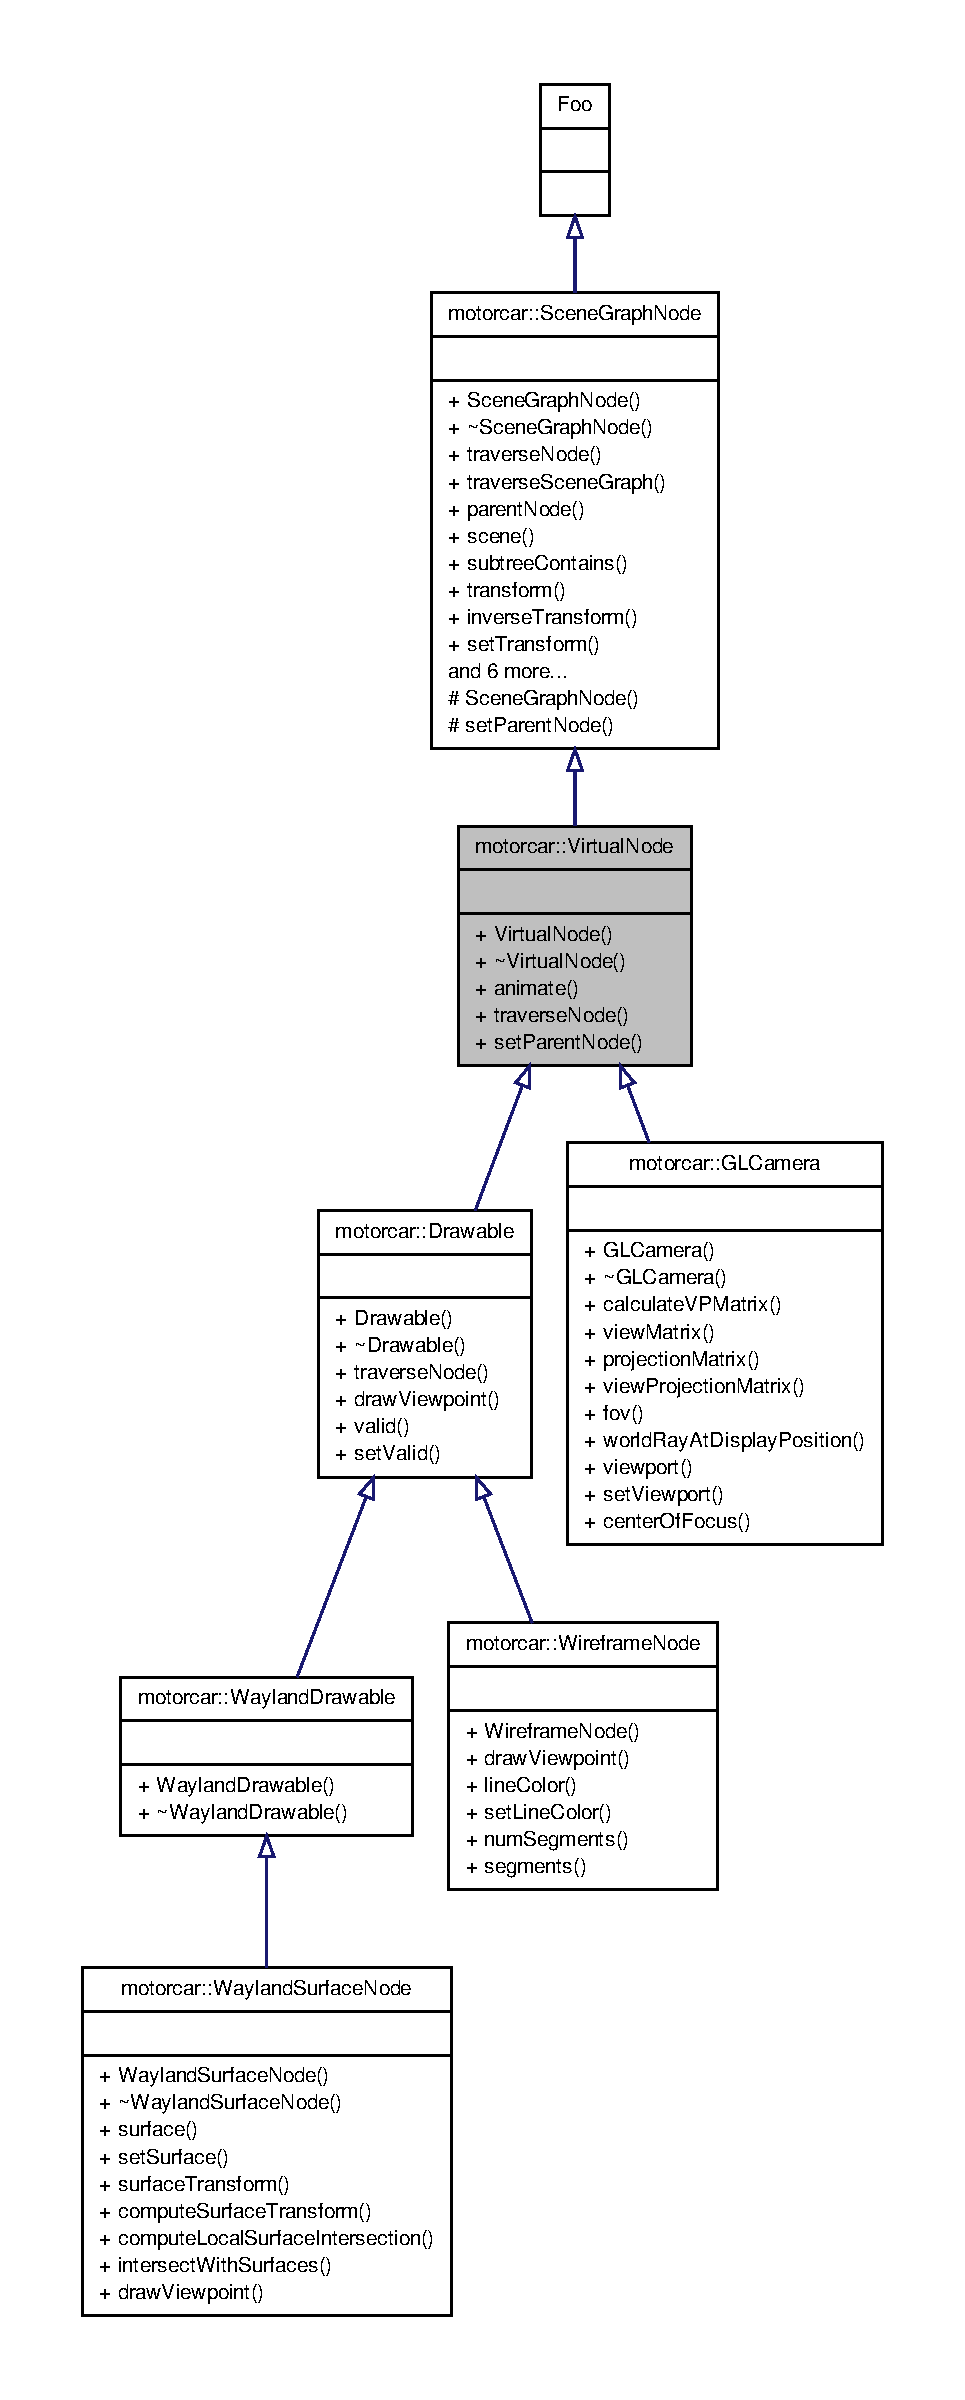
\includegraphics[width=350pt]{classmotorcar_1_1VirtualNode__inherit__graph}
\end{center}
\end{figure}


Collaboration diagram for motorcar\-:\-:Virtual\-Node\-:
\nopagebreak
\begin{figure}[H]
\begin{center}
\leavevmode
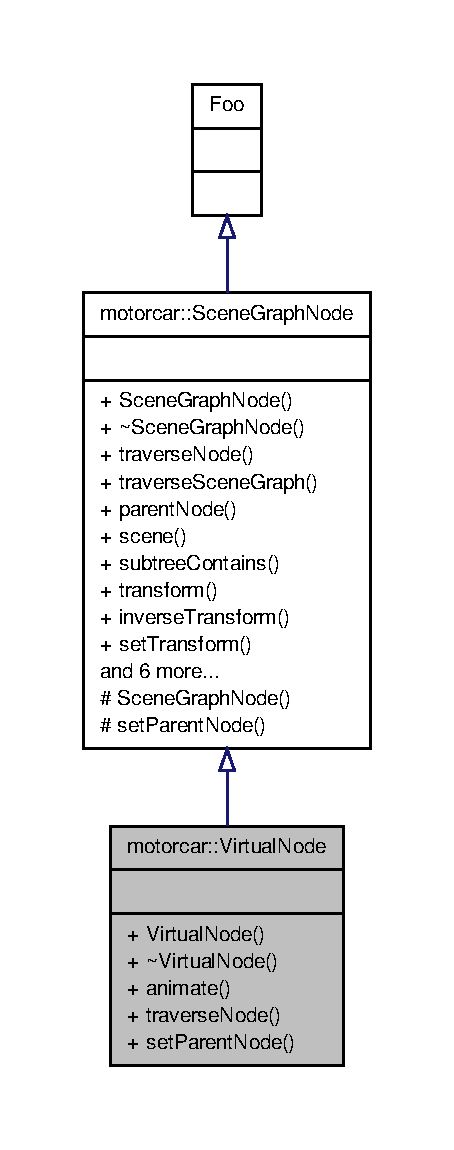
\includegraphics[width=218pt]{classmotorcar_1_1VirtualNode__coll__graph}
\end{center}
\end{figure}
\subsection*{Public Member Functions}
\begin{DoxyCompactItemize}
\item 
\hyperlink{classmotorcar_1_1VirtualNode_acee2e50a0321f81714a7984ce2effbbd}{Virtual\-Node} (\hyperlink{classmotorcar_1_1SceneGraphNode}{Scene\-Graph\-Node} $\ast$parent, const glm\-::mat4 \&\hyperlink{classmotorcar_1_1SceneGraphNode_ad96e79fdd739ac8223a3128003be391a}{transform}=glm\-::mat4())
\item 
virtual \hyperlink{classmotorcar_1_1VirtualNode_afb80a6d7b8ac5b3137357873d63a31c8}{$\sim$\-Virtual\-Node} ()
\item 
virtual void \hyperlink{classmotorcar_1_1VirtualNode_a43eca360af74fd3684a8f3d62a6aff35}{animate} (long delta\-Millis)
\item 
virtual void \hyperlink{classmotorcar_1_1VirtualNode_aae6c8f3752b46e84c65eb9fcab542f60}{handle\-Frame\-Begin} (\hyperlink{classmotorcar_1_1Scene}{Scene} $\ast$\hyperlink{classmotorcar_1_1SceneGraphNode_aa14e637ed4ae98f77e28941a4b5cfdd8}{scene}) override
\begin{DoxyCompactList}\small\item\em Set up the current node for the next frame. \end{DoxyCompactList}\item 
void \hyperlink{classmotorcar_1_1VirtualNode_aacea6d6974e649331232372d440b6505}{set\-Parent\-Node} (\hyperlink{classmotorcar_1_1SceneGraphNode}{Scene\-Graph\-Node} $\ast$parent)
\end{DoxyCompactItemize}
\subsection*{Additional Inherited Members}


\subsection{Constructor \& Destructor Documentation}
\hypertarget{classmotorcar_1_1VirtualNode_acee2e50a0321f81714a7984ce2effbbd}{\index{motorcar\-::\-Virtual\-Node@{motorcar\-::\-Virtual\-Node}!Virtual\-Node@{Virtual\-Node}}
\index{Virtual\-Node@{Virtual\-Node}!motorcar::VirtualNode@{motorcar\-::\-Virtual\-Node}}
\subsubsection[{Virtual\-Node}]{\setlength{\rightskip}{0pt plus 5cm}Virtual\-Node\-::\-Virtual\-Node (
\begin{DoxyParamCaption}
\item[{{\bf Scene\-Graph\-Node} $\ast$}]{parent, }
\item[{const glm\-::mat4 \&}]{transform = {\ttfamily glm\-:\-:mat4()}}
\end{DoxyParamCaption}
)}}\label{classmotorcar_1_1VirtualNode_acee2e50a0321f81714a7984ce2effbbd}
\hypertarget{classmotorcar_1_1VirtualNode_afb80a6d7b8ac5b3137357873d63a31c8}{\index{motorcar\-::\-Virtual\-Node@{motorcar\-::\-Virtual\-Node}!$\sim$\-Virtual\-Node@{$\sim$\-Virtual\-Node}}
\index{$\sim$\-Virtual\-Node@{$\sim$\-Virtual\-Node}!motorcar::VirtualNode@{motorcar\-::\-Virtual\-Node}}
\subsubsection[{$\sim$\-Virtual\-Node}]{\setlength{\rightskip}{0pt plus 5cm}virtual motorcar\-::\-Virtual\-Node\-::$\sim$\-Virtual\-Node (
\begin{DoxyParamCaption}
{}
\end{DoxyParamCaption}
)\hspace{0.3cm}{\ttfamily [inline]}, {\ttfamily [virtual]}}}\label{classmotorcar_1_1VirtualNode_afb80a6d7b8ac5b3137357873d63a31c8}


\subsection{Member Function Documentation}
\hypertarget{classmotorcar_1_1VirtualNode_a43eca360af74fd3684a8f3d62a6aff35}{\index{motorcar\-::\-Virtual\-Node@{motorcar\-::\-Virtual\-Node}!animate@{animate}}
\index{animate@{animate}!motorcar::VirtualNode@{motorcar\-::\-Virtual\-Node}}
\subsubsection[{animate}]{\setlength{\rightskip}{0pt plus 5cm}void Virtual\-Node\-::animate (
\begin{DoxyParamCaption}
\item[{long}]{delta\-Millis}
\end{DoxyParamCaption}
)\hspace{0.3cm}{\ttfamily [virtual]}}}\label{classmotorcar_1_1VirtualNode_a43eca360af74fd3684a8f3d62a6aff35}
\hypertarget{classmotorcar_1_1VirtualNode_aae6c8f3752b46e84c65eb9fcab542f60}{\index{motorcar\-::\-Virtual\-Node@{motorcar\-::\-Virtual\-Node}!handle\-Frame\-Begin@{handle\-Frame\-Begin}}
\index{handle\-Frame\-Begin@{handle\-Frame\-Begin}!motorcar::VirtualNode@{motorcar\-::\-Virtual\-Node}}
\subsubsection[{handle\-Frame\-Begin}]{\setlength{\rightskip}{0pt plus 5cm}void Virtual\-Node\-::handle\-Frame\-Begin (
\begin{DoxyParamCaption}
\item[{{\bf Scene} $\ast$}]{scene}
\end{DoxyParamCaption}
)\hspace{0.3cm}{\ttfamily [override]}, {\ttfamily [virtual]}}}\label{classmotorcar_1_1VirtualNode_aae6c8f3752b46e84c65eb9fcab542f60}


Set up the current node for the next frame. 



Reimplemented from \hyperlink{classmotorcar_1_1SceneGraphNode_a494eb20dd66a224888237af89ba6956f}{motorcar\-::\-Scene\-Graph\-Node}.



Reimplemented in \hyperlink{classmotorcar_1_1WaylandSurfaceNode_a7005bcd9c0944cec3b558344602c783e}{motorcar\-::\-Wayland\-Surface\-Node}.

\hypertarget{classmotorcar_1_1VirtualNode_aacea6d6974e649331232372d440b6505}{\index{motorcar\-::\-Virtual\-Node@{motorcar\-::\-Virtual\-Node}!set\-Parent\-Node@{set\-Parent\-Node}}
\index{set\-Parent\-Node@{set\-Parent\-Node}!motorcar::VirtualNode@{motorcar\-::\-Virtual\-Node}}
\subsubsection[{set\-Parent\-Node}]{\setlength{\rightskip}{0pt plus 5cm}void Virtual\-Node\-::set\-Parent\-Node (
\begin{DoxyParamCaption}
\item[{{\bf Scene\-Graph\-Node} $\ast$}]{parent}
\end{DoxyParamCaption}
)}}\label{classmotorcar_1_1VirtualNode_aacea6d6974e649331232372d440b6505}


The documentation for this class was generated from the following files\-:\begin{DoxyCompactItemize}
\item 
/media/dave/e89b5eb4-\/4b10-\/4edf-\/8ad5-\/0d046a46b978/dave/thesis/qtwayland-\/motorcar-\/compositor/motorcar/src/scenegraph/\hyperlink{virtualnode_8h}{virtualnode.\-h}\item 
/media/dave/e89b5eb4-\/4b10-\/4edf-\/8ad5-\/0d046a46b978/dave/thesis/qtwayland-\/motorcar-\/compositor/motorcar/src/scenegraph/\hyperlink{virtualnode_8cpp}{virtualnode.\-cpp}\end{DoxyCompactItemize}

\hypertarget{classmotorcar_1_1WaylandDrawable}{\section{motorcar\-:\-:Wayland\-Drawable Class Reference}
\label{classmotorcar_1_1WaylandDrawable}\index{motorcar\-::\-Wayland\-Drawable@{motorcar\-::\-Wayland\-Drawable}}
}


{\ttfamily \#include $<$waylanddrawable.\-h$>$}



Inheritance diagram for motorcar\-:\-:Wayland\-Drawable\-:
\nopagebreak
\begin{figure}[H]
\begin{center}
\leavevmode
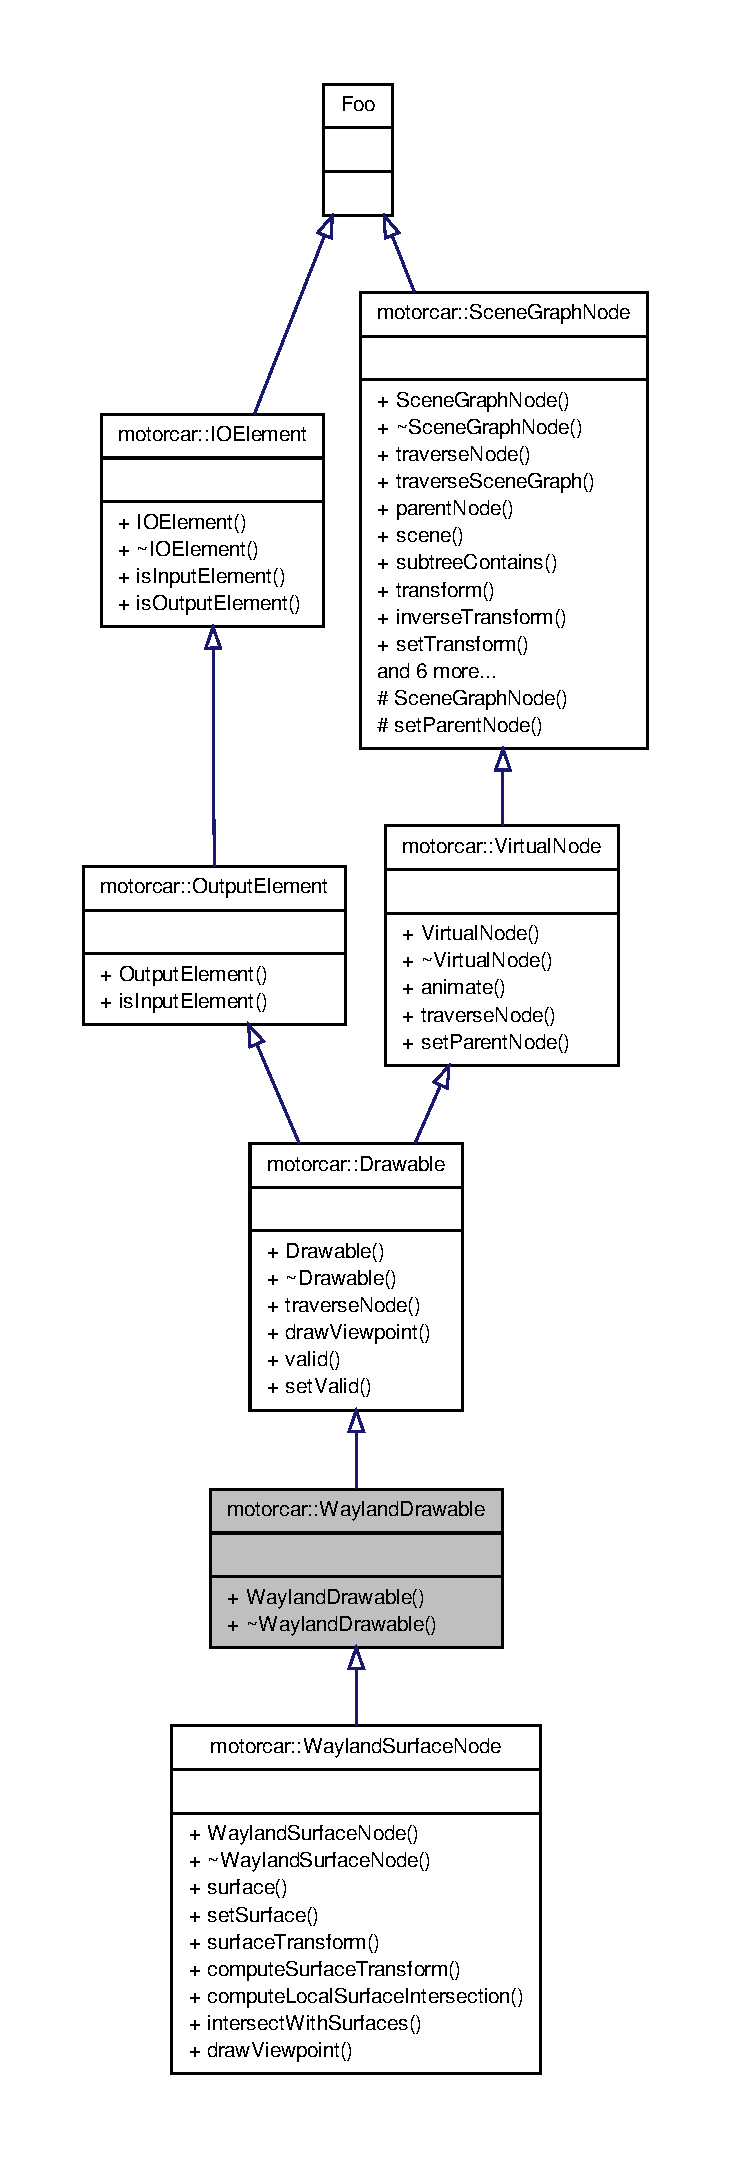
\includegraphics[height=550pt]{classmotorcar_1_1WaylandDrawable__inherit__graph}
\end{center}
\end{figure}


Collaboration diagram for motorcar\-:\-:Wayland\-Drawable\-:
\nopagebreak
\begin{figure}[H]
\begin{center}
\leavevmode
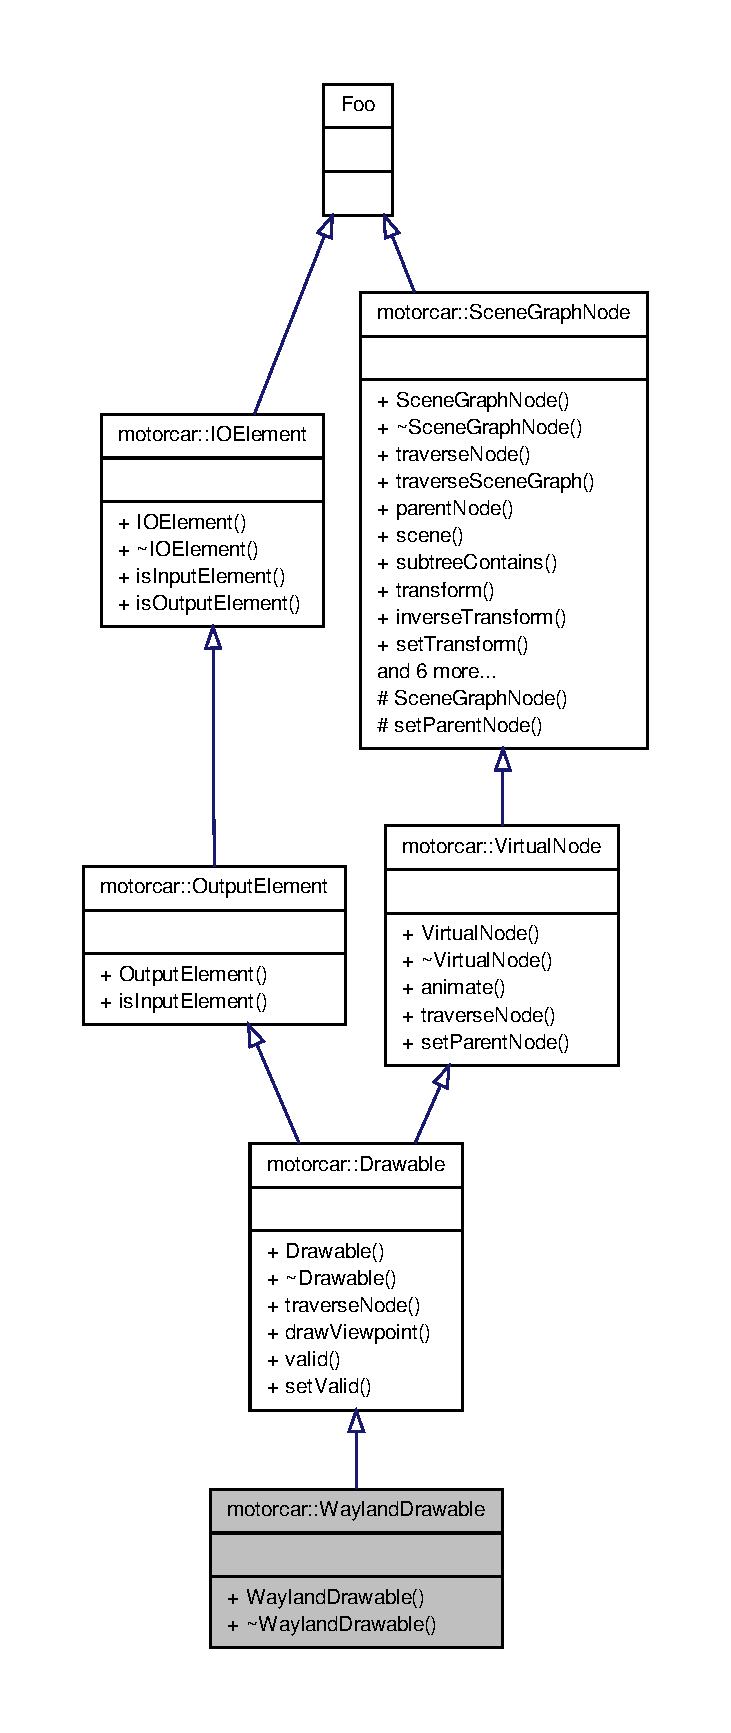
\includegraphics[height=550pt]{classmotorcar_1_1WaylandDrawable__coll__graph}
\end{center}
\end{figure}
\subsection*{Public Member Functions}
\begin{DoxyCompactItemize}
\item 
\hyperlink{classmotorcar_1_1WaylandDrawable_a8d8eb7dd37be10bf078f681be1d149f2}{Wayland\-Drawable} (\hyperlink{classmotorcar_1_1SceneGraphNode}{Scene\-Graph\-Node} $\ast$parent, const glm\-::mat4 \&\hyperlink{classmotorcar_1_1SceneGraphNode_ad96e79fdd739ac8223a3128003be391a}{transform}=glm\-::mat4(1))
\item 
virtual \hyperlink{classmotorcar_1_1WaylandDrawable_aacd6876953ab2a4488be95bb952411a8}{$\sim$\-Wayland\-Drawable} ()
\end{DoxyCompactItemize}
\subsection*{Additional Inherited Members}


\subsection{Constructor \& Destructor Documentation}
\hypertarget{classmotorcar_1_1WaylandDrawable_a8d8eb7dd37be10bf078f681be1d149f2}{\index{motorcar\-::\-Wayland\-Drawable@{motorcar\-::\-Wayland\-Drawable}!Wayland\-Drawable@{Wayland\-Drawable}}
\index{Wayland\-Drawable@{Wayland\-Drawable}!motorcar::WaylandDrawable@{motorcar\-::\-Wayland\-Drawable}}
\subsubsection[{Wayland\-Drawable}]{\setlength{\rightskip}{0pt plus 5cm}Wayland\-Drawable\-::\-Wayland\-Drawable (
\begin{DoxyParamCaption}
\item[{{\bf Scene\-Graph\-Node} $\ast$}]{parent, }
\item[{const glm\-::mat4 \&}]{transform = {\ttfamily glm\-:\-:mat4(1)}}
\end{DoxyParamCaption}
)}}\label{classmotorcar_1_1WaylandDrawable_a8d8eb7dd37be10bf078f681be1d149f2}
\hypertarget{classmotorcar_1_1WaylandDrawable_aacd6876953ab2a4488be95bb952411a8}{\index{motorcar\-::\-Wayland\-Drawable@{motorcar\-::\-Wayland\-Drawable}!$\sim$\-Wayland\-Drawable@{$\sim$\-Wayland\-Drawable}}
\index{$\sim$\-Wayland\-Drawable@{$\sim$\-Wayland\-Drawable}!motorcar::WaylandDrawable@{motorcar\-::\-Wayland\-Drawable}}
\subsubsection[{$\sim$\-Wayland\-Drawable}]{\setlength{\rightskip}{0pt plus 5cm}virtual motorcar\-::\-Wayland\-Drawable\-::$\sim$\-Wayland\-Drawable (
\begin{DoxyParamCaption}
{}
\end{DoxyParamCaption}
)\hspace{0.3cm}{\ttfamily [inline]}, {\ttfamily [virtual]}}}\label{classmotorcar_1_1WaylandDrawable_aacd6876953ab2a4488be95bb952411a8}


The documentation for this class was generated from the following files\-:\begin{DoxyCompactItemize}
\item 
/home/dave/thesis/qtwayland-\/motorcar-\/compositor/motorcar/src/scenegraph/output/wayland/\hyperlink{waylanddrawable_8h}{waylanddrawable.\-h}\item 
/home/dave/thesis/qtwayland-\/motorcar-\/compositor/motorcar/src/scenegraph/output/wayland/\hyperlink{waylanddrawable_8cpp}{waylanddrawable.\-cpp}\end{DoxyCompactItemize}

\hypertarget{classmotorcar_1_1WaylandSurface}{\section{motorcar\-:\-:Wayland\-Surface Class Reference}
\label{classmotorcar_1_1WaylandSurface}\index{motorcar\-::\-Wayland\-Surface@{motorcar\-::\-Wayland\-Surface}}
}


{\ttfamily \#include $<$waylandsurface.\-h$>$}



Inheritance diagram for motorcar\-:\-:Wayland\-Surface\-:
\nopagebreak
\begin{figure}[H]
\begin{center}
\leavevmode
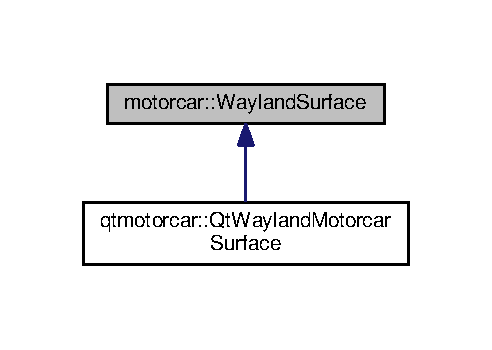
\includegraphics[width=236pt]{classmotorcar_1_1WaylandSurface__inherit__graph}
\end{center}
\end{figure}
\subsection*{Public Types}
\begin{DoxyCompactItemize}
\item 
enum \hyperlink{classmotorcar_1_1WaylandSurface_a7715a41b6776800656722407ec01e0a5}{Surface\-Type} \{ \\*
\hyperlink{classmotorcar_1_1WaylandSurface_a7715a41b6776800656722407ec01e0a5adc40004cddf6c1404780c88ad509cede}{T\-O\-P\-L\-E\-V\-E\-L}, 
\hyperlink{classmotorcar_1_1WaylandSurface_a7715a41b6776800656722407ec01e0a5a5a1e368e9f069279fec128c5ebf04ee5}{T\-R\-A\-N\-S\-I\-E\-N\-T}, 
\hyperlink{classmotorcar_1_1WaylandSurface_a7715a41b6776800656722407ec01e0a5a91f194806c8b59a53b1ea5ee47d567dc}{P\-O\-P\-U\-P}, 
\hyperlink{classmotorcar_1_1WaylandSurface_a7715a41b6776800656722407ec01e0a5a23d1dd5df19bc211c5835e285ec08a46}{C\-U\-R\-S\-O\-R}, 
\\*
\hyperlink{classmotorcar_1_1WaylandSurface_a7715a41b6776800656722407ec01e0a5a6577b08859e961558d1960bc03de1d51}{N\-A}
 \}
\item 
enum \hyperlink{classmotorcar_1_1WaylandSurface_ab48793c19a30e8ad689fb4465cd27a70}{Clipping\-Mode} \{ \hyperlink{classmotorcar_1_1WaylandSurface_ab48793c19a30e8ad689fb4465cd27a70a313e451685f55c86a28a58749d17f65a}{N\-O\-N\-E}, 
\hyperlink{classmotorcar_1_1WaylandSurface_ab48793c19a30e8ad689fb4465cd27a70a993d6596581174cec9ac557a0641e9fa}{C\-U\-B\-O\-I\-D}, 
\hyperlink{classmotorcar_1_1WaylandSurface_ab48793c19a30e8ad689fb4465cd27a70a84a3b7daf3ca3cf265a8966e96bb446c}{P\-O\-R\-T\-A\-L}
 \}
\end{DoxyCompactItemize}
\subsection*{Public Member Functions}
\begin{DoxyCompactItemize}
\item 
\hyperlink{classmotorcar_1_1WaylandSurface_a12a62c259b5041c6780c703ec2f12f01}{Wayland\-Surface} (\hyperlink{classmotorcar_1_1WaylandSurface_a7715a41b6776800656722407ec01e0a5}{Surface\-Type} \hyperlink{classmotorcar_1_1WaylandSurface_a0e6e5e2455666f607a8ddb2479ba8e88}{type}, bool \hyperlink{classmotorcar_1_1WaylandSurface_a9d7e9cbd9424831e8152bf70d395e397}{is\-Motorcar\-Surface}=false, \hyperlink{classmotorcar_1_1WaylandSurface_ab48793c19a30e8ad689fb4465cd27a70}{Clipping\-Mode} \hyperlink{classmotorcar_1_1WaylandSurface_add06f923d4bd62b3b3cb25d1e5f0ba0c}{clipping\-Mode}=Clipping\-Mode\-::\-N\-O\-N\-E, bool \hyperlink{classmotorcar_1_1WaylandSurface_a09cb70e037726ac4ee36c2aac9be30ae}{depth\-Compositing\-Enabled}=false)
\item 
virtual \hyperlink{classmotorcar_1_1WaylandSurface_a9b6ec8218ecc975308ddb38ddf3dd965}{$\sim$\-Wayland\-Surface} ()
\item 
virtual G\-Luint \hyperlink{classmotorcar_1_1WaylandSurface_aa8ae13d97dae8dfbb610ca6f4ab2b745}{texture} ()=0
\begin{DoxyCompactList}\small\item\em Get the texture handle for this surface. \end{DoxyCompactList}\item 
virtual glm\-::ivec2 \hyperlink{classmotorcar_1_1WaylandSurface_a06182d612aaf0d07780e498066aaca1b}{size} ()=0
\begin{DoxyCompactList}\small\item\em Get the size of this surface in pixels. \end{DoxyCompactList}\item 
virtual void \hyperlink{classmotorcar_1_1WaylandSurface_a7d2ee4e48305c5510916ba9bdcb46a44}{set\-Size} (glm\-::ivec2 new\-Size)=0
\begin{DoxyCompactList}\small\item\em Set the size of this surface in pixels. \end{DoxyCompactList}\item 
virtual glm\-::ivec2 \hyperlink{classmotorcar_1_1WaylandSurface_a22f62be59ac9b8b76a2b2f467f0b1277}{position} ()=0
\begin{DoxyCompactList}\small\item\em Get the position of this surface in parent surface-\/local coordinates. \end{DoxyCompactList}\item 
virtual \hyperlink{classmotorcar_1_1WaylandSurface}{Wayland\-Surface} $\ast$ \hyperlink{classmotorcar_1_1WaylandSurface_a94b48df54c92d9046f786d4d7f5d4ff2}{parent\-Surface} ()=0
\begin{DoxyCompactList}\small\item\em return the parent surface \end{DoxyCompactList}\item 
virtual void \hyperlink{classmotorcar_1_1WaylandSurface_a63669771c03ce580fec8a0099dbd294e}{prepare} ()=0
\begin{DoxyCompactList}\small\item\em do any per-\/frame setup required for drawing \end{DoxyCompactList}\item 
virtual bool \hyperlink{classmotorcar_1_1WaylandSurface_af2f54076ec690f4d478771183c9b0db5}{valid} ()=0
\begin{DoxyCompactList}\small\item\em returns whether or not the surface is ready to draw \end{DoxyCompactList}\item 
virtual void \hyperlink{classmotorcar_1_1WaylandSurface_a8d709e7d02ee7f7b8b3343590e518993}{send\-Event} (const \hyperlink{classmotorcar_1_1Event}{Event} \&event)=0
\item 
\hyperlink{classmotorcar_1_1WaylandSurface_a7715a41b6776800656722407ec01e0a5}{Surface\-Type} \hyperlink{classmotorcar_1_1WaylandSurface_a0e6e5e2455666f607a8ddb2479ba8e88}{type} () const 
\item 
void \hyperlink{classmotorcar_1_1WaylandSurface_a8806b03b3c4007578f26c1b907303336}{set\-Type} (const \hyperlink{classmotorcar_1_1WaylandSurface_a7715a41b6776800656722407ec01e0a5}{Surface\-Type} \&\hyperlink{classmotorcar_1_1WaylandSurface_a0e6e5e2455666f607a8ddb2479ba8e88}{type})
\item 
\hyperlink{classmotorcar_1_1WaylandSurface_ab48793c19a30e8ad689fb4465cd27a70}{Clipping\-Mode} \hyperlink{classmotorcar_1_1WaylandSurface_add06f923d4bd62b3b3cb25d1e5f0ba0c}{clipping\-Mode} () const 
\item 
void \hyperlink{classmotorcar_1_1WaylandSurface_ae0dcd1e480055dceb919b242089b59cb}{set\-Clipping\-Mode} (const \hyperlink{classmotorcar_1_1WaylandSurface_ab48793c19a30e8ad689fb4465cd27a70}{Wayland\-Surface\-::\-Clipping\-Mode} \&\hyperlink{classmotorcar_1_1WaylandSurface_add06f923d4bd62b3b3cb25d1e5f0ba0c}{clipping\-Mode})
\item 
bool \hyperlink{classmotorcar_1_1WaylandSurface_a09cb70e037726ac4ee36c2aac9be30ae}{depth\-Compositing\-Enabled} () const 
\item 
void \hyperlink{classmotorcar_1_1WaylandSurface_a8c51a8593ec8aff7862fd0cf7a6dc3a3}{set\-Depth\-Compositing\-Enabled} (bool \hyperlink{classmotorcar_1_1WaylandSurface_a09cb70e037726ac4ee36c2aac9be30ae}{depth\-Compositing\-Enabled})
\item 
bool \hyperlink{classmotorcar_1_1WaylandSurface_a9d7e9cbd9424831e8152bf70d395e397}{is\-Motorcar\-Surface} () const 
\item 
void \hyperlink{classmotorcar_1_1WaylandSurface_afcb5b959953f55f477315ecb47dcf484}{set\-Is\-Motorcar\-Surface} (bool \hyperlink{classmotorcar_1_1WaylandSurface_a9d7e9cbd9424831e8152bf70d395e397}{is\-Motorcar\-Surface})
\end{DoxyCompactItemize}
\subsection*{Protected Attributes}
\begin{DoxyCompactItemize}
\item 
\hyperlink{classmotorcar_1_1WaylandSurface_a7715a41b6776800656722407ec01e0a5}{Surface\-Type} \hyperlink{classmotorcar_1_1WaylandSurface_a73fc5c245e98a08a551c7f412fd95966}{m\-\_\-type}
\item 
\hyperlink{classmotorcar_1_1WaylandSurface_ab48793c19a30e8ad689fb4465cd27a70}{Clipping\-Mode} \hyperlink{classmotorcar_1_1WaylandSurface_a17668113470d8907fa0c6ef84758f828}{m\-\_\-clipping\-Mode}
\item 
bool \hyperlink{classmotorcar_1_1WaylandSurface_ae3f67aa2ac9bf4d7ebf54ada6b9152d0}{m\-\_\-depth\-Compositing\-Enabled}
\item 
bool \hyperlink{classmotorcar_1_1WaylandSurface_a123a2705782ddf461ab615362dcaeb89}{m\-\_\-is\-Motorcar\-Surface}
\end{DoxyCompactItemize}


\subsection{Member Enumeration Documentation}
\hypertarget{classmotorcar_1_1WaylandSurface_ab48793c19a30e8ad689fb4465cd27a70}{\index{motorcar\-::\-Wayland\-Surface@{motorcar\-::\-Wayland\-Surface}!Clipping\-Mode@{Clipping\-Mode}}
\index{Clipping\-Mode@{Clipping\-Mode}!motorcar::WaylandSurface@{motorcar\-::\-Wayland\-Surface}}
\subsubsection[{Clipping\-Mode}]{\setlength{\rightskip}{0pt plus 5cm}enum {\bf motorcar\-::\-Wayland\-Surface\-::\-Clipping\-Mode}}}\label{classmotorcar_1_1WaylandSurface_ab48793c19a30e8ad689fb4465cd27a70}
\begin{Desc}
\item[Enumerator]\par
\begin{description}
\index{N\-O\-N\-E@{N\-O\-N\-E}!motorcar\-::\-Wayland\-Surface@{motorcar\-::\-Wayland\-Surface}}\index{motorcar\-::\-Wayland\-Surface@{motorcar\-::\-Wayland\-Surface}!N\-O\-N\-E@{N\-O\-N\-E}}\item[{\em 
\hypertarget{classmotorcar_1_1WaylandSurface_ab48793c19a30e8ad689fb4465cd27a70a313e451685f55c86a28a58749d17f65a}{N\-O\-N\-E}\label{classmotorcar_1_1WaylandSurface_ab48793c19a30e8ad689fb4465cd27a70a313e451685f55c86a28a58749d17f65a}
}]\index{C\-U\-B\-O\-I\-D@{C\-U\-B\-O\-I\-D}!motorcar\-::\-Wayland\-Surface@{motorcar\-::\-Wayland\-Surface}}\index{motorcar\-::\-Wayland\-Surface@{motorcar\-::\-Wayland\-Surface}!C\-U\-B\-O\-I\-D@{C\-U\-B\-O\-I\-D}}\item[{\em 
\hypertarget{classmotorcar_1_1WaylandSurface_ab48793c19a30e8ad689fb4465cd27a70a993d6596581174cec9ac557a0641e9fa}{C\-U\-B\-O\-I\-D}\label{classmotorcar_1_1WaylandSurface_ab48793c19a30e8ad689fb4465cd27a70a993d6596581174cec9ac557a0641e9fa}
}]\index{P\-O\-R\-T\-A\-L@{P\-O\-R\-T\-A\-L}!motorcar\-::\-Wayland\-Surface@{motorcar\-::\-Wayland\-Surface}}\index{motorcar\-::\-Wayland\-Surface@{motorcar\-::\-Wayland\-Surface}!P\-O\-R\-T\-A\-L@{P\-O\-R\-T\-A\-L}}\item[{\em 
\hypertarget{classmotorcar_1_1WaylandSurface_ab48793c19a30e8ad689fb4465cd27a70a84a3b7daf3ca3cf265a8966e96bb446c}{P\-O\-R\-T\-A\-L}\label{classmotorcar_1_1WaylandSurface_ab48793c19a30e8ad689fb4465cd27a70a84a3b7daf3ca3cf265a8966e96bb446c}
}]\end{description}
\end{Desc}
\hypertarget{classmotorcar_1_1WaylandSurface_a7715a41b6776800656722407ec01e0a5}{\index{motorcar\-::\-Wayland\-Surface@{motorcar\-::\-Wayland\-Surface}!Surface\-Type@{Surface\-Type}}
\index{Surface\-Type@{Surface\-Type}!motorcar::WaylandSurface@{motorcar\-::\-Wayland\-Surface}}
\subsubsection[{Surface\-Type}]{\setlength{\rightskip}{0pt plus 5cm}enum {\bf motorcar\-::\-Wayland\-Surface\-::\-Surface\-Type}}}\label{classmotorcar_1_1WaylandSurface_a7715a41b6776800656722407ec01e0a5}
\begin{Desc}
\item[Enumerator]\par
\begin{description}
\index{T\-O\-P\-L\-E\-V\-E\-L@{T\-O\-P\-L\-E\-V\-E\-L}!motorcar\-::\-Wayland\-Surface@{motorcar\-::\-Wayland\-Surface}}\index{motorcar\-::\-Wayland\-Surface@{motorcar\-::\-Wayland\-Surface}!T\-O\-P\-L\-E\-V\-E\-L@{T\-O\-P\-L\-E\-V\-E\-L}}\item[{\em 
\hypertarget{classmotorcar_1_1WaylandSurface_a7715a41b6776800656722407ec01e0a5adc40004cddf6c1404780c88ad509cede}{T\-O\-P\-L\-E\-V\-E\-L}\label{classmotorcar_1_1WaylandSurface_a7715a41b6776800656722407ec01e0a5adc40004cddf6c1404780c88ad509cede}
}]\index{T\-R\-A\-N\-S\-I\-E\-N\-T@{T\-R\-A\-N\-S\-I\-E\-N\-T}!motorcar\-::\-Wayland\-Surface@{motorcar\-::\-Wayland\-Surface}}\index{motorcar\-::\-Wayland\-Surface@{motorcar\-::\-Wayland\-Surface}!T\-R\-A\-N\-S\-I\-E\-N\-T@{T\-R\-A\-N\-S\-I\-E\-N\-T}}\item[{\em 
\hypertarget{classmotorcar_1_1WaylandSurface_a7715a41b6776800656722407ec01e0a5a5a1e368e9f069279fec128c5ebf04ee5}{T\-R\-A\-N\-S\-I\-E\-N\-T}\label{classmotorcar_1_1WaylandSurface_a7715a41b6776800656722407ec01e0a5a5a1e368e9f069279fec128c5ebf04ee5}
}]\index{P\-O\-P\-U\-P@{P\-O\-P\-U\-P}!motorcar\-::\-Wayland\-Surface@{motorcar\-::\-Wayland\-Surface}}\index{motorcar\-::\-Wayland\-Surface@{motorcar\-::\-Wayland\-Surface}!P\-O\-P\-U\-P@{P\-O\-P\-U\-P}}\item[{\em 
\hypertarget{classmotorcar_1_1WaylandSurface_a7715a41b6776800656722407ec01e0a5a91f194806c8b59a53b1ea5ee47d567dc}{P\-O\-P\-U\-P}\label{classmotorcar_1_1WaylandSurface_a7715a41b6776800656722407ec01e0a5a91f194806c8b59a53b1ea5ee47d567dc}
}]\index{C\-U\-R\-S\-O\-R@{C\-U\-R\-S\-O\-R}!motorcar\-::\-Wayland\-Surface@{motorcar\-::\-Wayland\-Surface}}\index{motorcar\-::\-Wayland\-Surface@{motorcar\-::\-Wayland\-Surface}!C\-U\-R\-S\-O\-R@{C\-U\-R\-S\-O\-R}}\item[{\em 
\hypertarget{classmotorcar_1_1WaylandSurface_a7715a41b6776800656722407ec01e0a5a23d1dd5df19bc211c5835e285ec08a46}{C\-U\-R\-S\-O\-R}\label{classmotorcar_1_1WaylandSurface_a7715a41b6776800656722407ec01e0a5a23d1dd5df19bc211c5835e285ec08a46}
}]\index{N\-A@{N\-A}!motorcar\-::\-Wayland\-Surface@{motorcar\-::\-Wayland\-Surface}}\index{motorcar\-::\-Wayland\-Surface@{motorcar\-::\-Wayland\-Surface}!N\-A@{N\-A}}\item[{\em 
\hypertarget{classmotorcar_1_1WaylandSurface_a7715a41b6776800656722407ec01e0a5a6577b08859e961558d1960bc03de1d51}{N\-A}\label{classmotorcar_1_1WaylandSurface_a7715a41b6776800656722407ec01e0a5a6577b08859e961558d1960bc03de1d51}
}]\end{description}
\end{Desc}


\subsection{Constructor \& Destructor Documentation}
\hypertarget{classmotorcar_1_1WaylandSurface_a12a62c259b5041c6780c703ec2f12f01}{\index{motorcar\-::\-Wayland\-Surface@{motorcar\-::\-Wayland\-Surface}!Wayland\-Surface@{Wayland\-Surface}}
\index{Wayland\-Surface@{Wayland\-Surface}!motorcar::WaylandSurface@{motorcar\-::\-Wayland\-Surface}}
\subsubsection[{Wayland\-Surface}]{\setlength{\rightskip}{0pt plus 5cm}Wayland\-Surface\-::\-Wayland\-Surface (
\begin{DoxyParamCaption}
\item[{{\bf Surface\-Type}}]{type, }
\item[{bool}]{is\-Motorcar\-Surface = {\ttfamily false}, }
\item[{{\bf Clipping\-Mode}}]{clipping\-Mode = {\ttfamily ClippingMode\-:\-:NONE}, }
\item[{bool}]{depth\-Compositing\-Enabled = {\ttfamily false}}
\end{DoxyParamCaption}
)}}\label{classmotorcar_1_1WaylandSurface_a12a62c259b5041c6780c703ec2f12f01}
\hypertarget{classmotorcar_1_1WaylandSurface_a9b6ec8218ecc975308ddb38ddf3dd965}{\index{motorcar\-::\-Wayland\-Surface@{motorcar\-::\-Wayland\-Surface}!$\sim$\-Wayland\-Surface@{$\sim$\-Wayland\-Surface}}
\index{$\sim$\-Wayland\-Surface@{$\sim$\-Wayland\-Surface}!motorcar::WaylandSurface@{motorcar\-::\-Wayland\-Surface}}
\subsubsection[{$\sim$\-Wayland\-Surface}]{\setlength{\rightskip}{0pt plus 5cm}virtual motorcar\-::\-Wayland\-Surface\-::$\sim$\-Wayland\-Surface (
\begin{DoxyParamCaption}
{}
\end{DoxyParamCaption}
)\hspace{0.3cm}{\ttfamily [inline]}, {\ttfamily [virtual]}}}\label{classmotorcar_1_1WaylandSurface_a9b6ec8218ecc975308ddb38ddf3dd965}


\subsection{Member Function Documentation}
\hypertarget{classmotorcar_1_1WaylandSurface_add06f923d4bd62b3b3cb25d1e5f0ba0c}{\index{motorcar\-::\-Wayland\-Surface@{motorcar\-::\-Wayland\-Surface}!clipping\-Mode@{clipping\-Mode}}
\index{clipping\-Mode@{clipping\-Mode}!motorcar::WaylandSurface@{motorcar\-::\-Wayland\-Surface}}
\subsubsection[{clipping\-Mode}]{\setlength{\rightskip}{0pt plus 5cm}{\bf Wayland\-Surface\-::\-Clipping\-Mode} Wayland\-Surface\-::clipping\-Mode (
\begin{DoxyParamCaption}
{}
\end{DoxyParamCaption}
) const}}\label{classmotorcar_1_1WaylandSurface_add06f923d4bd62b3b3cb25d1e5f0ba0c}
\hypertarget{classmotorcar_1_1WaylandSurface_a09cb70e037726ac4ee36c2aac9be30ae}{\index{motorcar\-::\-Wayland\-Surface@{motorcar\-::\-Wayland\-Surface}!depth\-Compositing\-Enabled@{depth\-Compositing\-Enabled}}
\index{depth\-Compositing\-Enabled@{depth\-Compositing\-Enabled}!motorcar::WaylandSurface@{motorcar\-::\-Wayland\-Surface}}
\subsubsection[{depth\-Compositing\-Enabled}]{\setlength{\rightskip}{0pt plus 5cm}bool Wayland\-Surface\-::depth\-Compositing\-Enabled (
\begin{DoxyParamCaption}
{}
\end{DoxyParamCaption}
) const}}\label{classmotorcar_1_1WaylandSurface_a09cb70e037726ac4ee36c2aac9be30ae}
\hypertarget{classmotorcar_1_1WaylandSurface_a9d7e9cbd9424831e8152bf70d395e397}{\index{motorcar\-::\-Wayland\-Surface@{motorcar\-::\-Wayland\-Surface}!is\-Motorcar\-Surface@{is\-Motorcar\-Surface}}
\index{is\-Motorcar\-Surface@{is\-Motorcar\-Surface}!motorcar::WaylandSurface@{motorcar\-::\-Wayland\-Surface}}
\subsubsection[{is\-Motorcar\-Surface}]{\setlength{\rightskip}{0pt plus 5cm}bool Wayland\-Surface\-::is\-Motorcar\-Surface (
\begin{DoxyParamCaption}
{}
\end{DoxyParamCaption}
) const}}\label{classmotorcar_1_1WaylandSurface_a9d7e9cbd9424831e8152bf70d395e397}
\hypertarget{classmotorcar_1_1WaylandSurface_a94b48df54c92d9046f786d4d7f5d4ff2}{\index{motorcar\-::\-Wayland\-Surface@{motorcar\-::\-Wayland\-Surface}!parent\-Surface@{parent\-Surface}}
\index{parent\-Surface@{parent\-Surface}!motorcar::WaylandSurface@{motorcar\-::\-Wayland\-Surface}}
\subsubsection[{parent\-Surface}]{\setlength{\rightskip}{0pt plus 5cm}virtual {\bf Wayland\-Surface}$\ast$ motorcar\-::\-Wayland\-Surface\-::parent\-Surface (
\begin{DoxyParamCaption}
{}
\end{DoxyParamCaption}
)\hspace{0.3cm}{\ttfamily [pure virtual]}}}\label{classmotorcar_1_1WaylandSurface_a94b48df54c92d9046f786d4d7f5d4ff2}


return the parent surface 



Implemented in \hyperlink{classqtmotorcar_1_1QtWaylandMotorcarSurface_a3b0aed06d7ed9287497bc342f9fc787b}{qtmotorcar\-::\-Qt\-Wayland\-Motorcar\-Surface}.

\hypertarget{classmotorcar_1_1WaylandSurface_a22f62be59ac9b8b76a2b2f467f0b1277}{\index{motorcar\-::\-Wayland\-Surface@{motorcar\-::\-Wayland\-Surface}!position@{position}}
\index{position@{position}!motorcar::WaylandSurface@{motorcar\-::\-Wayland\-Surface}}
\subsubsection[{position}]{\setlength{\rightskip}{0pt plus 5cm}virtual glm\-::ivec2 motorcar\-::\-Wayland\-Surface\-::position (
\begin{DoxyParamCaption}
{}
\end{DoxyParamCaption}
)\hspace{0.3cm}{\ttfamily [pure virtual]}}}\label{classmotorcar_1_1WaylandSurface_a22f62be59ac9b8b76a2b2f467f0b1277}


Get the position of this surface in parent surface-\/local coordinates. 



Implemented in \hyperlink{classqtmotorcar_1_1QtWaylandMotorcarSurface_ad405b91565405e6a08d86ac5d59f3f08}{qtmotorcar\-::\-Qt\-Wayland\-Motorcar\-Surface}.

\hypertarget{classmotorcar_1_1WaylandSurface_a63669771c03ce580fec8a0099dbd294e}{\index{motorcar\-::\-Wayland\-Surface@{motorcar\-::\-Wayland\-Surface}!prepare@{prepare}}
\index{prepare@{prepare}!motorcar::WaylandSurface@{motorcar\-::\-Wayland\-Surface}}
\subsubsection[{prepare}]{\setlength{\rightskip}{0pt plus 5cm}virtual void motorcar\-::\-Wayland\-Surface\-::prepare (
\begin{DoxyParamCaption}
{}
\end{DoxyParamCaption}
)\hspace{0.3cm}{\ttfamily [pure virtual]}}}\label{classmotorcar_1_1WaylandSurface_a63669771c03ce580fec8a0099dbd294e}


do any per-\/frame setup required for drawing 



Implemented in \hyperlink{classqtmotorcar_1_1QtWaylandMotorcarSurface_ae898706dcf80a2f00ed2477c570dcebe}{qtmotorcar\-::\-Qt\-Wayland\-Motorcar\-Surface}.

\hypertarget{classmotorcar_1_1WaylandSurface_a8d709e7d02ee7f7b8b3343590e518993}{\index{motorcar\-::\-Wayland\-Surface@{motorcar\-::\-Wayland\-Surface}!send\-Event@{send\-Event}}
\index{send\-Event@{send\-Event}!motorcar::WaylandSurface@{motorcar\-::\-Wayland\-Surface}}
\subsubsection[{send\-Event}]{\setlength{\rightskip}{0pt plus 5cm}virtual void motorcar\-::\-Wayland\-Surface\-::send\-Event (
\begin{DoxyParamCaption}
\item[{const {\bf Event} \&}]{event}
\end{DoxyParamCaption}
)\hspace{0.3cm}{\ttfamily [pure virtual]}}}\label{classmotorcar_1_1WaylandSurface_a8d709e7d02ee7f7b8b3343590e518993}


Implemented in \hyperlink{classqtmotorcar_1_1QtWaylandMotorcarSurface_a7deebcf58954f82c8d5741af054414a7}{qtmotorcar\-::\-Qt\-Wayland\-Motorcar\-Surface}.

\hypertarget{classmotorcar_1_1WaylandSurface_ae0dcd1e480055dceb919b242089b59cb}{\index{motorcar\-::\-Wayland\-Surface@{motorcar\-::\-Wayland\-Surface}!set\-Clipping\-Mode@{set\-Clipping\-Mode}}
\index{set\-Clipping\-Mode@{set\-Clipping\-Mode}!motorcar::WaylandSurface@{motorcar\-::\-Wayland\-Surface}}
\subsubsection[{set\-Clipping\-Mode}]{\setlength{\rightskip}{0pt plus 5cm}void Wayland\-Surface\-::set\-Clipping\-Mode (
\begin{DoxyParamCaption}
\item[{const {\bf Wayland\-Surface\-::\-Clipping\-Mode} \&}]{clipping\-Mode}
\end{DoxyParamCaption}
)}}\label{classmotorcar_1_1WaylandSurface_ae0dcd1e480055dceb919b242089b59cb}
\hypertarget{classmotorcar_1_1WaylandSurface_a8c51a8593ec8aff7862fd0cf7a6dc3a3}{\index{motorcar\-::\-Wayland\-Surface@{motorcar\-::\-Wayland\-Surface}!set\-Depth\-Compositing\-Enabled@{set\-Depth\-Compositing\-Enabled}}
\index{set\-Depth\-Compositing\-Enabled@{set\-Depth\-Compositing\-Enabled}!motorcar::WaylandSurface@{motorcar\-::\-Wayland\-Surface}}
\subsubsection[{set\-Depth\-Compositing\-Enabled}]{\setlength{\rightskip}{0pt plus 5cm}void Wayland\-Surface\-::set\-Depth\-Compositing\-Enabled (
\begin{DoxyParamCaption}
\item[{bool}]{depth\-Compositing\-Enabled}
\end{DoxyParamCaption}
)}}\label{classmotorcar_1_1WaylandSurface_a8c51a8593ec8aff7862fd0cf7a6dc3a3}
\hypertarget{classmotorcar_1_1WaylandSurface_afcb5b959953f55f477315ecb47dcf484}{\index{motorcar\-::\-Wayland\-Surface@{motorcar\-::\-Wayland\-Surface}!set\-Is\-Motorcar\-Surface@{set\-Is\-Motorcar\-Surface}}
\index{set\-Is\-Motorcar\-Surface@{set\-Is\-Motorcar\-Surface}!motorcar::WaylandSurface@{motorcar\-::\-Wayland\-Surface}}
\subsubsection[{set\-Is\-Motorcar\-Surface}]{\setlength{\rightskip}{0pt plus 5cm}void Wayland\-Surface\-::set\-Is\-Motorcar\-Surface (
\begin{DoxyParamCaption}
\item[{bool}]{is\-Motorcar\-Surface}
\end{DoxyParamCaption}
)}}\label{classmotorcar_1_1WaylandSurface_afcb5b959953f55f477315ecb47dcf484}
\hypertarget{classmotorcar_1_1WaylandSurface_a7d2ee4e48305c5510916ba9bdcb46a44}{\index{motorcar\-::\-Wayland\-Surface@{motorcar\-::\-Wayland\-Surface}!set\-Size@{set\-Size}}
\index{set\-Size@{set\-Size}!motorcar::WaylandSurface@{motorcar\-::\-Wayland\-Surface}}
\subsubsection[{set\-Size}]{\setlength{\rightskip}{0pt plus 5cm}virtual void motorcar\-::\-Wayland\-Surface\-::set\-Size (
\begin{DoxyParamCaption}
\item[{glm\-::ivec2}]{new\-Size}
\end{DoxyParamCaption}
)\hspace{0.3cm}{\ttfamily [pure virtual]}}}\label{classmotorcar_1_1WaylandSurface_a7d2ee4e48305c5510916ba9bdcb46a44}


Set the size of this surface in pixels. 



Implemented in \hyperlink{classqtmotorcar_1_1QtWaylandMotorcarSurface_abb0d9d5b6a226ab201fc1c0065d1843a}{qtmotorcar\-::\-Qt\-Wayland\-Motorcar\-Surface}.

\hypertarget{classmotorcar_1_1WaylandSurface_a8806b03b3c4007578f26c1b907303336}{\index{motorcar\-::\-Wayland\-Surface@{motorcar\-::\-Wayland\-Surface}!set\-Type@{set\-Type}}
\index{set\-Type@{set\-Type}!motorcar::WaylandSurface@{motorcar\-::\-Wayland\-Surface}}
\subsubsection[{set\-Type}]{\setlength{\rightskip}{0pt plus 5cm}void Wayland\-Surface\-::set\-Type (
\begin{DoxyParamCaption}
\item[{const {\bf Surface\-Type} \&}]{type}
\end{DoxyParamCaption}
)}}\label{classmotorcar_1_1WaylandSurface_a8806b03b3c4007578f26c1b907303336}
\hypertarget{classmotorcar_1_1WaylandSurface_a06182d612aaf0d07780e498066aaca1b}{\index{motorcar\-::\-Wayland\-Surface@{motorcar\-::\-Wayland\-Surface}!size@{size}}
\index{size@{size}!motorcar::WaylandSurface@{motorcar\-::\-Wayland\-Surface}}
\subsubsection[{size}]{\setlength{\rightskip}{0pt plus 5cm}virtual glm\-::ivec2 motorcar\-::\-Wayland\-Surface\-::size (
\begin{DoxyParamCaption}
{}
\end{DoxyParamCaption}
)\hspace{0.3cm}{\ttfamily [pure virtual]}}}\label{classmotorcar_1_1WaylandSurface_a06182d612aaf0d07780e498066aaca1b}


Get the size of this surface in pixels. 



Implemented in \hyperlink{classqtmotorcar_1_1QtWaylandMotorcarSurface_ad5e6f75c146a2952652deaf866ee22a7}{qtmotorcar\-::\-Qt\-Wayland\-Motorcar\-Surface}.

\hypertarget{classmotorcar_1_1WaylandSurface_aa8ae13d97dae8dfbb610ca6f4ab2b745}{\index{motorcar\-::\-Wayland\-Surface@{motorcar\-::\-Wayland\-Surface}!texture@{texture}}
\index{texture@{texture}!motorcar::WaylandSurface@{motorcar\-::\-Wayland\-Surface}}
\subsubsection[{texture}]{\setlength{\rightskip}{0pt plus 5cm}virtual G\-Luint motorcar\-::\-Wayland\-Surface\-::texture (
\begin{DoxyParamCaption}
{}
\end{DoxyParamCaption}
)\hspace{0.3cm}{\ttfamily [pure virtual]}}}\label{classmotorcar_1_1WaylandSurface_aa8ae13d97dae8dfbb610ca6f4ab2b745}


Get the texture handle for this surface. 



Implemented in \hyperlink{classqtmotorcar_1_1QtWaylandMotorcarSurface_a573c52cdacb8f16c06ecd111bddabef6}{qtmotorcar\-::\-Qt\-Wayland\-Motorcar\-Surface}.

\hypertarget{classmotorcar_1_1WaylandSurface_a0e6e5e2455666f607a8ddb2479ba8e88}{\index{motorcar\-::\-Wayland\-Surface@{motorcar\-::\-Wayland\-Surface}!type@{type}}
\index{type@{type}!motorcar::WaylandSurface@{motorcar\-::\-Wayland\-Surface}}
\subsubsection[{type}]{\setlength{\rightskip}{0pt plus 5cm}{\bf Wayland\-Surface\-::\-Surface\-Type} Wayland\-Surface\-::type (
\begin{DoxyParamCaption}
{}
\end{DoxyParamCaption}
) const}}\label{classmotorcar_1_1WaylandSurface_a0e6e5e2455666f607a8ddb2479ba8e88}
\hypertarget{classmotorcar_1_1WaylandSurface_af2f54076ec690f4d478771183c9b0db5}{\index{motorcar\-::\-Wayland\-Surface@{motorcar\-::\-Wayland\-Surface}!valid@{valid}}
\index{valid@{valid}!motorcar::WaylandSurface@{motorcar\-::\-Wayland\-Surface}}
\subsubsection[{valid}]{\setlength{\rightskip}{0pt plus 5cm}virtual bool motorcar\-::\-Wayland\-Surface\-::valid (
\begin{DoxyParamCaption}
{}
\end{DoxyParamCaption}
)\hspace{0.3cm}{\ttfamily [pure virtual]}}}\label{classmotorcar_1_1WaylandSurface_af2f54076ec690f4d478771183c9b0db5}


returns whether or not the surface is ready to draw 



Implemented in \hyperlink{classqtmotorcar_1_1QtWaylandMotorcarSurface_a3bea85a2a6a3079e60c3b37dd08aebc6}{qtmotorcar\-::\-Qt\-Wayland\-Motorcar\-Surface}.



\subsection{Member Data Documentation}
\hypertarget{classmotorcar_1_1WaylandSurface_a17668113470d8907fa0c6ef84758f828}{\index{motorcar\-::\-Wayland\-Surface@{motorcar\-::\-Wayland\-Surface}!m\-\_\-clipping\-Mode@{m\-\_\-clipping\-Mode}}
\index{m\-\_\-clipping\-Mode@{m\-\_\-clipping\-Mode}!motorcar::WaylandSurface@{motorcar\-::\-Wayland\-Surface}}
\subsubsection[{m\-\_\-clipping\-Mode}]{\setlength{\rightskip}{0pt plus 5cm}{\bf Clipping\-Mode} motorcar\-::\-Wayland\-Surface\-::m\-\_\-clipping\-Mode\hspace{0.3cm}{\ttfamily [protected]}}}\label{classmotorcar_1_1WaylandSurface_a17668113470d8907fa0c6ef84758f828}
\hypertarget{classmotorcar_1_1WaylandSurface_ae3f67aa2ac9bf4d7ebf54ada6b9152d0}{\index{motorcar\-::\-Wayland\-Surface@{motorcar\-::\-Wayland\-Surface}!m\-\_\-depth\-Compositing\-Enabled@{m\-\_\-depth\-Compositing\-Enabled}}
\index{m\-\_\-depth\-Compositing\-Enabled@{m\-\_\-depth\-Compositing\-Enabled}!motorcar::WaylandSurface@{motorcar\-::\-Wayland\-Surface}}
\subsubsection[{m\-\_\-depth\-Compositing\-Enabled}]{\setlength{\rightskip}{0pt plus 5cm}bool motorcar\-::\-Wayland\-Surface\-::m\-\_\-depth\-Compositing\-Enabled\hspace{0.3cm}{\ttfamily [protected]}}}\label{classmotorcar_1_1WaylandSurface_ae3f67aa2ac9bf4d7ebf54ada6b9152d0}
\hypertarget{classmotorcar_1_1WaylandSurface_a123a2705782ddf461ab615362dcaeb89}{\index{motorcar\-::\-Wayland\-Surface@{motorcar\-::\-Wayland\-Surface}!m\-\_\-is\-Motorcar\-Surface@{m\-\_\-is\-Motorcar\-Surface}}
\index{m\-\_\-is\-Motorcar\-Surface@{m\-\_\-is\-Motorcar\-Surface}!motorcar::WaylandSurface@{motorcar\-::\-Wayland\-Surface}}
\subsubsection[{m\-\_\-is\-Motorcar\-Surface}]{\setlength{\rightskip}{0pt plus 5cm}bool motorcar\-::\-Wayland\-Surface\-::m\-\_\-is\-Motorcar\-Surface\hspace{0.3cm}{\ttfamily [protected]}}}\label{classmotorcar_1_1WaylandSurface_a123a2705782ddf461ab615362dcaeb89}
\hypertarget{classmotorcar_1_1WaylandSurface_a73fc5c245e98a08a551c7f412fd95966}{\index{motorcar\-::\-Wayland\-Surface@{motorcar\-::\-Wayland\-Surface}!m\-\_\-type@{m\-\_\-type}}
\index{m\-\_\-type@{m\-\_\-type}!motorcar::WaylandSurface@{motorcar\-::\-Wayland\-Surface}}
\subsubsection[{m\-\_\-type}]{\setlength{\rightskip}{0pt plus 5cm}{\bf Surface\-Type} motorcar\-::\-Wayland\-Surface\-::m\-\_\-type\hspace{0.3cm}{\ttfamily [protected]}}}\label{classmotorcar_1_1WaylandSurface_a73fc5c245e98a08a551c7f412fd95966}


The documentation for this class was generated from the following files\-:\begin{DoxyCompactItemize}
\item 
/home/dave/thesis/motorcar/src/compositor/wayland/output/\hyperlink{waylandsurface_8h}{waylandsurface.\-h}\item 
/home/dave/thesis/motorcar/src/compositor/wayland/output/\hyperlink{waylandsurface_8cpp}{waylandsurface.\-cpp}\end{DoxyCompactItemize}

\hypertarget{classmotorcar_1_1WaylandSurfaceNode}{\section{motorcar\-:\-:Wayland\-Surface\-Node Class Reference}
\label{classmotorcar_1_1WaylandSurfaceNode}\index{motorcar\-::\-Wayland\-Surface\-Node@{motorcar\-::\-Wayland\-Surface\-Node}}
}


{\ttfamily \#include $<$waylandsurfacenode.\-h$>$}



Inheritance diagram for motorcar\-:\-:Wayland\-Surface\-Node\-:
\nopagebreak
\begin{figure}[H]
\begin{center}
\leavevmode
\includegraphics[height=550pt]{classmotorcar_1_1WaylandSurfaceNode__inherit__graph}
\end{center}
\end{figure}


Collaboration diagram for motorcar\-:\-:Wayland\-Surface\-Node\-:
\nopagebreak
\begin{figure}[H]
\begin{center}
\leavevmode
\includegraphics[height=550pt]{classmotorcar_1_1WaylandSurfaceNode__coll__graph}
\end{center}
\end{figure}
\subsection*{Public Member Functions}
\begin{DoxyCompactItemize}
\item 
\hyperlink{classmotorcar_1_1WaylandSurfaceNode_ad7d045ae80caac6164e293ba5c7e9307}{Wayland\-Surface\-Node} (\hyperlink{classmotorcar_1_1WaylandSurface}{Wayland\-Surface} $\ast$\hyperlink{classmotorcar_1_1WaylandSurfaceNode_a2f888be4621ed73d815ce006246f50ca}{surface}, \hyperlink{classmotorcar_1_1SceneGraphNode}{Scene\-Graph\-Node} $\ast$parent, const glm\-::mat4 \&\hyperlink{classmotorcar_1_1SceneGraphNode_ad96e79fdd739ac8223a3128003be391a}{transform}=glm\-::mat4(1))
\item 
virtual \hyperlink{classmotorcar_1_1WaylandSurfaceNode_aa5b4593dd0f4834a4d8e1416f322ac8f}{$\sim$\-Wayland\-Surface\-Node} ()
\item 
\hyperlink{classmotorcar_1_1WaylandSurface}{Wayland\-Surface} $\ast$ \hyperlink{classmotorcar_1_1WaylandSurfaceNode_a2f888be4621ed73d815ce006246f50ca}{surface} () const 
\item 
void \hyperlink{classmotorcar_1_1WaylandSurfaceNode_ae073a9e9f05bd5d62f09d24f9a86a31a}{set\-Surface} (\hyperlink{classmotorcar_1_1WaylandSurface}{Wayland\-Surface} $\ast$\hyperlink{classmotorcar_1_1WaylandSurfaceNode_a2f888be4621ed73d815ce006246f50ca}{surface})
\item 
glm\-::mat4 \hyperlink{classmotorcar_1_1WaylandSurfaceNode_a3910d8ccc764aed402074f21c25a89e8}{surface\-Transform} () const 
\item 
void \hyperlink{classmotorcar_1_1WaylandSurfaceNode_a0dfac06ca2855e41613b6e663c76c97e}{compute\-Surface\-Transform} (float ppcm)
\item 
bool \hyperlink{classmotorcar_1_1WaylandSurfaceNode_a7830bc430977685b9d22732171f30dcf}{compute\-Local\-Surface\-Intersection} (const \hyperlink{structmotorcar_1_1Geometry_1_1Ray}{Geometry\-::\-Ray} \&local\-Ray, glm\-::vec2 \&local\-Intersection, float \&t)
\item 
virtual \\*
\hyperlink{structmotorcar_1_1Geometry_1_1RaySurfaceIntersection}{Geometry\-::\-Ray\-Surface\-Intersection} $\ast$ \hyperlink{classmotorcar_1_1WaylandSurfaceNode_adf71a714d07bb262405a361504a77ea4}{intersect\-With\-Surfaces} (const \hyperlink{structmotorcar_1_1Geometry_1_1Ray}{Geometry\-::\-Ray} \&ray) override
\item 
void \hyperlink{classmotorcar_1_1WaylandSurfaceNode_a74d79ca15a4d7983a29752fad8db574c}{draw\-Viewpoint} (\hyperlink{classmotorcar_1_1GLCamera}{G\-L\-Camera} $\ast$viewpoint) override
\end{DoxyCompactItemize}
\subsection*{Additional Inherited Members}


\subsection{Constructor \& Destructor Documentation}
\hypertarget{classmotorcar_1_1WaylandSurfaceNode_ad7d045ae80caac6164e293ba5c7e9307}{\index{motorcar\-::\-Wayland\-Surface\-Node@{motorcar\-::\-Wayland\-Surface\-Node}!Wayland\-Surface\-Node@{Wayland\-Surface\-Node}}
\index{Wayland\-Surface\-Node@{Wayland\-Surface\-Node}!motorcar::WaylandSurfaceNode@{motorcar\-::\-Wayland\-Surface\-Node}}
\subsubsection[{Wayland\-Surface\-Node}]{\setlength{\rightskip}{0pt plus 5cm}Wayland\-Surface\-Node\-::\-Wayland\-Surface\-Node (
\begin{DoxyParamCaption}
\item[{{\bf Wayland\-Surface} $\ast$}]{surface, }
\item[{{\bf Scene\-Graph\-Node} $\ast$}]{parent, }
\item[{const glm\-::mat4 \&}]{transform = {\ttfamily glm\-:\-:mat4(1)}}
\end{DoxyParamCaption}
)}}\label{classmotorcar_1_1WaylandSurfaceNode_ad7d045ae80caac6164e293ba5c7e9307}
\hypertarget{classmotorcar_1_1WaylandSurfaceNode_aa5b4593dd0f4834a4d8e1416f322ac8f}{\index{motorcar\-::\-Wayland\-Surface\-Node@{motorcar\-::\-Wayland\-Surface\-Node}!$\sim$\-Wayland\-Surface\-Node@{$\sim$\-Wayland\-Surface\-Node}}
\index{$\sim$\-Wayland\-Surface\-Node@{$\sim$\-Wayland\-Surface\-Node}!motorcar::WaylandSurfaceNode@{motorcar\-::\-Wayland\-Surface\-Node}}
\subsubsection[{$\sim$\-Wayland\-Surface\-Node}]{\setlength{\rightskip}{0pt plus 5cm}Wayland\-Surface\-Node\-::$\sim$\-Wayland\-Surface\-Node (
\begin{DoxyParamCaption}
{}
\end{DoxyParamCaption}
)\hspace{0.3cm}{\ttfamily [virtual]}}}\label{classmotorcar_1_1WaylandSurfaceNode_aa5b4593dd0f4834a4d8e1416f322ac8f}


\subsection{Member Function Documentation}
\hypertarget{classmotorcar_1_1WaylandSurfaceNode_a7830bc430977685b9d22732171f30dcf}{\index{motorcar\-::\-Wayland\-Surface\-Node@{motorcar\-::\-Wayland\-Surface\-Node}!compute\-Local\-Surface\-Intersection@{compute\-Local\-Surface\-Intersection}}
\index{compute\-Local\-Surface\-Intersection@{compute\-Local\-Surface\-Intersection}!motorcar::WaylandSurfaceNode@{motorcar\-::\-Wayland\-Surface\-Node}}
\subsubsection[{compute\-Local\-Surface\-Intersection}]{\setlength{\rightskip}{0pt plus 5cm}bool Wayland\-Surface\-Node\-::compute\-Local\-Surface\-Intersection (
\begin{DoxyParamCaption}
\item[{const {\bf Geometry\-::\-Ray} \&}]{local\-Ray, }
\item[{glm\-::vec2 \&}]{local\-Intersection, }
\item[{float \&}]{t}
\end{DoxyParamCaption}
)}}\label{classmotorcar_1_1WaylandSurfaceNode_a7830bc430977685b9d22732171f30dcf}
\hypertarget{classmotorcar_1_1WaylandSurfaceNode_a0dfac06ca2855e41613b6e663c76c97e}{\index{motorcar\-::\-Wayland\-Surface\-Node@{motorcar\-::\-Wayland\-Surface\-Node}!compute\-Surface\-Transform@{compute\-Surface\-Transform}}
\index{compute\-Surface\-Transform@{compute\-Surface\-Transform}!motorcar::WaylandSurfaceNode@{motorcar\-::\-Wayland\-Surface\-Node}}
\subsubsection[{compute\-Surface\-Transform}]{\setlength{\rightskip}{0pt plus 5cm}void Wayland\-Surface\-Node\-::compute\-Surface\-Transform (
\begin{DoxyParamCaption}
\item[{float}]{ppcm}
\end{DoxyParamCaption}
)}}\label{classmotorcar_1_1WaylandSurfaceNode_a0dfac06ca2855e41613b6e663c76c97e}
\hypertarget{classmotorcar_1_1WaylandSurfaceNode_a74d79ca15a4d7983a29752fad8db574c}{\index{motorcar\-::\-Wayland\-Surface\-Node@{motorcar\-::\-Wayland\-Surface\-Node}!draw\-Viewpoint@{draw\-Viewpoint}}
\index{draw\-Viewpoint@{draw\-Viewpoint}!motorcar::WaylandSurfaceNode@{motorcar\-::\-Wayland\-Surface\-Node}}
\subsubsection[{draw\-Viewpoint}]{\setlength{\rightskip}{0pt plus 5cm}void Wayland\-Surface\-Node\-::draw\-Viewpoint (
\begin{DoxyParamCaption}
\item[{{\bf G\-L\-Camera} $\ast$}]{viewpoint}
\end{DoxyParamCaption}
)\hspace{0.3cm}{\ttfamily [override]}, {\ttfamily [virtual]}}}\label{classmotorcar_1_1WaylandSurfaceNode_a74d79ca15a4d7983a29752fad8db574c}


Implements \hyperlink{classmotorcar_1_1Drawable_aa991a852cb0421ecef23669df01b5b62}{motorcar\-::\-Drawable}.

\hypertarget{classmotorcar_1_1WaylandSurfaceNode_adf71a714d07bb262405a361504a77ea4}{\index{motorcar\-::\-Wayland\-Surface\-Node@{motorcar\-::\-Wayland\-Surface\-Node}!intersect\-With\-Surfaces@{intersect\-With\-Surfaces}}
\index{intersect\-With\-Surfaces@{intersect\-With\-Surfaces}!motorcar::WaylandSurfaceNode@{motorcar\-::\-Wayland\-Surface\-Node}}
\subsubsection[{intersect\-With\-Surfaces}]{\setlength{\rightskip}{0pt plus 5cm}{\bf Geometry\-::\-Ray\-Surface\-Intersection} $\ast$ Wayland\-Surface\-Node\-::intersect\-With\-Surfaces (
\begin{DoxyParamCaption}
\item[{const {\bf Geometry\-::\-Ray} \&}]{ray}
\end{DoxyParamCaption}
)\hspace{0.3cm}{\ttfamily [override]}, {\ttfamily [virtual]}}}\label{classmotorcar_1_1WaylandSurfaceNode_adf71a714d07bb262405a361504a77ea4}


Reimplemented from \hyperlink{classmotorcar_1_1SceneGraphNode_ac268b171317430368fcc7733eab05ae6}{motorcar\-::\-Scene\-Graph\-Node}.

\hypertarget{classmotorcar_1_1WaylandSurfaceNode_ae073a9e9f05bd5d62f09d24f9a86a31a}{\index{motorcar\-::\-Wayland\-Surface\-Node@{motorcar\-::\-Wayland\-Surface\-Node}!set\-Surface@{set\-Surface}}
\index{set\-Surface@{set\-Surface}!motorcar::WaylandSurfaceNode@{motorcar\-::\-Wayland\-Surface\-Node}}
\subsubsection[{set\-Surface}]{\setlength{\rightskip}{0pt plus 5cm}void Wayland\-Surface\-Node\-::set\-Surface (
\begin{DoxyParamCaption}
\item[{{\bf Wayland\-Surface} $\ast$}]{surface}
\end{DoxyParamCaption}
)}}\label{classmotorcar_1_1WaylandSurfaceNode_ae073a9e9f05bd5d62f09d24f9a86a31a}
\hypertarget{classmotorcar_1_1WaylandSurfaceNode_a2f888be4621ed73d815ce006246f50ca}{\index{motorcar\-::\-Wayland\-Surface\-Node@{motorcar\-::\-Wayland\-Surface\-Node}!surface@{surface}}
\index{surface@{surface}!motorcar::WaylandSurfaceNode@{motorcar\-::\-Wayland\-Surface\-Node}}
\subsubsection[{surface}]{\setlength{\rightskip}{0pt plus 5cm}{\bf Wayland\-Surface} $\ast$ Wayland\-Surface\-Node\-::surface (
\begin{DoxyParamCaption}
{}
\end{DoxyParamCaption}
) const}}\label{classmotorcar_1_1WaylandSurfaceNode_a2f888be4621ed73d815ce006246f50ca}
\hypertarget{classmotorcar_1_1WaylandSurfaceNode_a3910d8ccc764aed402074f21c25a89e8}{\index{motorcar\-::\-Wayland\-Surface\-Node@{motorcar\-::\-Wayland\-Surface\-Node}!surface\-Transform@{surface\-Transform}}
\index{surface\-Transform@{surface\-Transform}!motorcar::WaylandSurfaceNode@{motorcar\-::\-Wayland\-Surface\-Node}}
\subsubsection[{surface\-Transform}]{\setlength{\rightskip}{0pt plus 5cm}glm\-::mat4 Wayland\-Surface\-Node\-::surface\-Transform (
\begin{DoxyParamCaption}
{}
\end{DoxyParamCaption}
) const}}\label{classmotorcar_1_1WaylandSurfaceNode_a3910d8ccc764aed402074f21c25a89e8}


The documentation for this class was generated from the following files\-:\begin{DoxyCompactItemize}
\item 
/home/dave/thesis/qtwayland-\/motorcar-\/compositor/motorcar/src/scenegraph/output/wayland/\hyperlink{waylandsurfacenode_8h}{waylandsurfacenode.\-h}\item 
/home/dave/thesis/qtwayland-\/motorcar-\/compositor/motorcar/src/scenegraph/output/wayland/\hyperlink{waylandsurfacenode_8cpp}{waylandsurfacenode.\-cpp}\end{DoxyCompactItemize}

\hypertarget{classmotorcar_1_1WireframeNode}{\section{motorcar\-:\-:Wireframe\-Node Class Reference}
\label{classmotorcar_1_1WireframeNode}\index{motorcar\-::\-Wireframe\-Node@{motorcar\-::\-Wireframe\-Node}}
}


{\ttfamily \#include $<$wireframenode.\-h$>$}



Inheritance diagram for motorcar\-:\-:Wireframe\-Node\-:
\nopagebreak
\begin{figure}[H]
\begin{center}
\leavevmode
\includegraphics[height=550pt]{classmotorcar_1_1WireframeNode__inherit__graph}
\end{center}
\end{figure}


Collaboration diagram for motorcar\-:\-:Wireframe\-Node\-:
\nopagebreak
\begin{figure}[H]
\begin{center}
\leavevmode
\includegraphics[height=550pt]{classmotorcar_1_1WireframeNode__coll__graph}
\end{center}
\end{figure}
\subsection*{Public Member Functions}
\begin{DoxyCompactItemize}
\item 
\hyperlink{classmotorcar_1_1WireframeNode_aa20d4f27da8395ba0d12f8fb0aa3631b}{Wireframe\-Node} (float $\ast$\hyperlink{classmotorcar_1_1WireframeNode_aedf65e6feb6cebaa7cf0e95819386a72}{segments}, int \hyperlink{classmotorcar_1_1WireframeNode_aeffe078a56d3a162de14e26a96bc474d}{num\-Segments}, glm\-::vec3 \hyperlink{classmotorcar_1_1WireframeNode_a70dd1214503a3650d6a919cb6b7c5313}{line\-Color}, \hyperlink{classmotorcar_1_1SceneGraphNode}{Scene\-Graph\-Node} $\ast$parent, const glm\-::mat4 \&\hyperlink{classmotorcar_1_1SceneGraphNode_ad96e79fdd739ac8223a3128003be391a}{transform}=glm\-::mat4())
\item 
void \hyperlink{classmotorcar_1_1WireframeNode_a9256807100fb8d169d7f4e1c657463d7}{draw\-Viewpoint} (\hyperlink{classmotorcar_1_1GLCamera}{G\-L\-Camera} $\ast$viewpoint) override
\item 
glm\-::vec3 \hyperlink{classmotorcar_1_1WireframeNode_a70dd1214503a3650d6a919cb6b7c5313}{line\-Color} () const 
\item 
void \hyperlink{classmotorcar_1_1WireframeNode_a915a448da09b9cb24ecdeec38ee8a8a9}{set\-Line\-Color} (const glm\-::vec3 \&\hyperlink{classmotorcar_1_1WireframeNode_a70dd1214503a3650d6a919cb6b7c5313}{line\-Color})
\item 
int \hyperlink{classmotorcar_1_1WireframeNode_aeffe078a56d3a162de14e26a96bc474d}{num\-Segments} () const 
\item 
float $\ast$ \hyperlink{classmotorcar_1_1WireframeNode_aedf65e6feb6cebaa7cf0e95819386a72}{segments} () const 
\end{DoxyCompactItemize}
\subsection*{Additional Inherited Members}


\subsection{Constructor \& Destructor Documentation}
\hypertarget{classmotorcar_1_1WireframeNode_aa20d4f27da8395ba0d12f8fb0aa3631b}{\index{motorcar\-::\-Wireframe\-Node@{motorcar\-::\-Wireframe\-Node}!Wireframe\-Node@{Wireframe\-Node}}
\index{Wireframe\-Node@{Wireframe\-Node}!motorcar::WireframeNode@{motorcar\-::\-Wireframe\-Node}}
\subsubsection[{Wireframe\-Node}]{\setlength{\rightskip}{0pt plus 5cm}Wireframe\-Node\-::\-Wireframe\-Node (
\begin{DoxyParamCaption}
\item[{float $\ast$}]{segments, }
\item[{int}]{num\-Segments, }
\item[{glm\-::vec3}]{line\-Color, }
\item[{{\bf Scene\-Graph\-Node} $\ast$}]{parent, }
\item[{const glm\-::mat4 \&}]{transform = {\ttfamily glm\-:\-:mat4()}}
\end{DoxyParamCaption}
)}}\label{classmotorcar_1_1WireframeNode_aa20d4f27da8395ba0d12f8fb0aa3631b}


\subsection{Member Function Documentation}
\hypertarget{classmotorcar_1_1WireframeNode_a9256807100fb8d169d7f4e1c657463d7}{\index{motorcar\-::\-Wireframe\-Node@{motorcar\-::\-Wireframe\-Node}!draw\-Viewpoint@{draw\-Viewpoint}}
\index{draw\-Viewpoint@{draw\-Viewpoint}!motorcar::WireframeNode@{motorcar\-::\-Wireframe\-Node}}
\subsubsection[{draw\-Viewpoint}]{\setlength{\rightskip}{0pt plus 5cm}void Wireframe\-Node\-::draw\-Viewpoint (
\begin{DoxyParamCaption}
\item[{{\bf G\-L\-Camera} $\ast$}]{viewpoint}
\end{DoxyParamCaption}
)\hspace{0.3cm}{\ttfamily [override]}, {\ttfamily [virtual]}}}\label{classmotorcar_1_1WireframeNode_a9256807100fb8d169d7f4e1c657463d7}


Implements \hyperlink{classmotorcar_1_1Drawable_aa991a852cb0421ecef23669df01b5b62}{motorcar\-::\-Drawable}.

\hypertarget{classmotorcar_1_1WireframeNode_a70dd1214503a3650d6a919cb6b7c5313}{\index{motorcar\-::\-Wireframe\-Node@{motorcar\-::\-Wireframe\-Node}!line\-Color@{line\-Color}}
\index{line\-Color@{line\-Color}!motorcar::WireframeNode@{motorcar\-::\-Wireframe\-Node}}
\subsubsection[{line\-Color}]{\setlength{\rightskip}{0pt plus 5cm}glm\-::vec3 Wireframe\-Node\-::line\-Color (
\begin{DoxyParamCaption}
{}
\end{DoxyParamCaption}
) const}}\label{classmotorcar_1_1WireframeNode_a70dd1214503a3650d6a919cb6b7c5313}
\hypertarget{classmotorcar_1_1WireframeNode_aeffe078a56d3a162de14e26a96bc474d}{\index{motorcar\-::\-Wireframe\-Node@{motorcar\-::\-Wireframe\-Node}!num\-Segments@{num\-Segments}}
\index{num\-Segments@{num\-Segments}!motorcar::WireframeNode@{motorcar\-::\-Wireframe\-Node}}
\subsubsection[{num\-Segments}]{\setlength{\rightskip}{0pt plus 5cm}int Wireframe\-Node\-::num\-Segments (
\begin{DoxyParamCaption}
{}
\end{DoxyParamCaption}
) const}}\label{classmotorcar_1_1WireframeNode_aeffe078a56d3a162de14e26a96bc474d}
\hypertarget{classmotorcar_1_1WireframeNode_aedf65e6feb6cebaa7cf0e95819386a72}{\index{motorcar\-::\-Wireframe\-Node@{motorcar\-::\-Wireframe\-Node}!segments@{segments}}
\index{segments@{segments}!motorcar::WireframeNode@{motorcar\-::\-Wireframe\-Node}}
\subsubsection[{segments}]{\setlength{\rightskip}{0pt plus 5cm}float $\ast$ Wireframe\-Node\-::segments (
\begin{DoxyParamCaption}
{}
\end{DoxyParamCaption}
) const}}\label{classmotorcar_1_1WireframeNode_aedf65e6feb6cebaa7cf0e95819386a72}
\hypertarget{classmotorcar_1_1WireframeNode_a915a448da09b9cb24ecdeec38ee8a8a9}{\index{motorcar\-::\-Wireframe\-Node@{motorcar\-::\-Wireframe\-Node}!set\-Line\-Color@{set\-Line\-Color}}
\index{set\-Line\-Color@{set\-Line\-Color}!motorcar::WireframeNode@{motorcar\-::\-Wireframe\-Node}}
\subsubsection[{set\-Line\-Color}]{\setlength{\rightskip}{0pt plus 5cm}void Wireframe\-Node\-::set\-Line\-Color (
\begin{DoxyParamCaption}
\item[{const glm\-::vec3 \&}]{line\-Color}
\end{DoxyParamCaption}
)}}\label{classmotorcar_1_1WireframeNode_a915a448da09b9cb24ecdeec38ee8a8a9}


The documentation for this class was generated from the following files\-:\begin{DoxyCompactItemize}
\item 
/home/dave/thesis/qtwayland-\/motorcar-\/compositor/motorcar/src/scenegraph/output/\hyperlink{wireframenode_8h}{wireframenode.\-h}\item 
/home/dave/thesis/qtwayland-\/motorcar-\/compositor/motorcar/src/scenegraph/output/\hyperlink{wireframenode_8cpp}{wireframenode.\-cpp}\end{DoxyCompactItemize}

\chapter{File Documentation}
\hypertarget{compositor_8cpp}{\section{/home/dave/thesis/motorcar/src/compositor/compositor.cpp File Reference}
\label{compositor_8cpp}\index{/home/dave/thesis/motorcar/src/compositor/compositor.\-cpp@{/home/dave/thesis/motorcar/src/compositor/compositor.\-cpp}}
}
{\ttfamily \#include $<$compositor.\-h$>$}\\*
{\ttfamily \#include $<$qt/qtwaylandmotorcarcompositor.\-h$>$}\\*
Include dependency graph for compositor.\-cpp\-:
\nopagebreak
\begin{figure}[H]
\begin{center}
\leavevmode
\includegraphics[width=350pt]{compositor_8cpp__incl}
\end{center}
\end{figure}

\hypertarget{compositor_8h}{\section{/home/dave/thesis/qtwayland-\/motorcar-\/compositor/motorcar/src/compositor.h File Reference}
\label{compositor_8h}\index{/home/dave/thesis/qtwayland-\/motorcar-\/compositor/motorcar/src/compositor.\-h@{/home/dave/thesis/qtwayland-\/motorcar-\/compositor/motorcar/src/compositor.\-h}}
}
{\ttfamily \#include \char`\"{}scenegraph/output/display/display.\-h\char`\"{}}\\*
{\ttfamily \#include \char`\"{}gl/openglcontext.\-h\char`\"{}}\\*
Include dependency graph for compositor.\-h\-:
\nopagebreak
\begin{figure}[H]
\begin{center}
\leavevmode
\includegraphics[width=350pt]{compositor_8h__incl}
\end{center}
\end{figure}
This graph shows which files directly or indirectly include this file\-:
\nopagebreak
\begin{figure}[H]
\begin{center}
\leavevmode
\includegraphics[width=350pt]{compositor_8h__dep__incl}
\end{center}
\end{figure}
\subsection*{Classes}
\begin{DoxyCompactItemize}
\item 
class \hyperlink{classmotorcar_1_1Compositor}{motorcar\-::\-Compositor}
\end{DoxyCompactItemize}
\subsection*{Namespaces}
\begin{DoxyCompactItemize}
\item 
\hyperlink{namespacemotorcar}{motorcar}
\end{DoxyCompactItemize}
\subsection*{Constant Groups}
\begin{DoxyCompactItemize}
\item 
\hyperlink{namespacemotorcar}{motorcar}
\end{DoxyCompactItemize}

\hypertarget{device_8h}{\section{/media/dave/e89b5eb4-\/4b10-\/4edf-\/8ad5-\/0d046a46b978/dave/thesis/qtwayland-\/motorcar-\/compositor/motorcar/src/device/device.h File Reference}
\label{device_8h}\index{/media/dave/e89b5eb4-\/4b10-\/4edf-\/8ad5-\/0d046a46b978/dave/thesis/qtwayland-\/motorcar-\/compositor/motorcar/src/device/device.\-h@{/media/dave/e89b5eb4-\/4b10-\/4edf-\/8ad5-\/0d046a46b978/dave/thesis/qtwayland-\/motorcar-\/compositor/motorcar/src/device/device.\-h}}
}
{\ttfamily \#include \char`\"{}oculushmd.\-h\char`\"{}}\\*
{\ttfamily \#include \char`\"{}sixensecontrollernode.\-h\char`\"{}}\\*
{\ttfamily \#include \char`\"{}sixensemotionsensingsystem.\-h\char`\"{}}\\*
{\ttfamily \#include \char`\"{}softkineticdepthcamera.\-h\char`\"{}}\\*
Include dependency graph for device.\-h\-:\nopagebreak
\begin{figure}[H]
\begin{center}
\leavevmode
\includegraphics[width=350pt]{device_8h__incl}
\end{center}
\end{figure}
This graph shows which files directly or indirectly include this file\-:\nopagebreak
\begin{figure}[H]
\begin{center}
\leavevmode
\includegraphics[width=276pt]{device_8h__dep__incl}
\end{center}
\end{figure}

\hypertarget{oculushmd_8cpp}{\section{/media/dave/e89b5eb4-\/4b10-\/4edf-\/8ad5-\/0d046a46b978/dave/thesis/qtwayland-\/motorcar-\/compositor/motorcar/src/device/oculushmd.cpp File Reference}
\label{oculushmd_8cpp}\index{/media/dave/e89b5eb4-\/4b10-\/4edf-\/8ad5-\/0d046a46b978/dave/thesis/qtwayland-\/motorcar-\/compositor/motorcar/src/device/oculushmd.\-cpp@{/media/dave/e89b5eb4-\/4b10-\/4edf-\/8ad5-\/0d046a46b978/dave/thesis/qtwayland-\/motorcar-\/compositor/motorcar/src/device/oculushmd.\-cpp}}
}
{\ttfamily \#include \char`\"{}oculushmd.\-h\char`\"{}}\\*
Include dependency graph for oculushmd.\-cpp\-:\nopagebreak
\begin{figure}[H]
\begin{center}
\leavevmode
\includegraphics[width=350pt]{oculushmd_8cpp__incl}
\end{center}
\end{figure}

\hypertarget{oculushmd_8h}{\section{/home/dave/thesis/qtwayland-\/motorcar-\/compositor/motorcar/src/device/oculushmd.h File Reference}
\label{oculushmd_8h}\index{/home/dave/thesis/qtwayland-\/motorcar-\/compositor/motorcar/src/device/oculushmd.\-h@{/home/dave/thesis/qtwayland-\/motorcar-\/compositor/motorcar/src/device/oculushmd.\-h}}
}
{\ttfamily \#include \char`\"{}../scenegraph/output/display/rendertotexturedisplay.\-h\char`\"{}}\\*
{\ttfamily \#include \char`\"{}O\-V\-R.\-h\char`\"{}}\\*
Include dependency graph for oculushmd.\-h\-:
\nopagebreak
\begin{figure}[H]
\begin{center}
\leavevmode
\includegraphics[width=350pt]{oculushmd_8h__incl}
\end{center}
\end{figure}
This graph shows which files directly or indirectly include this file\-:
\nopagebreak
\begin{figure}[H]
\begin{center}
\leavevmode
\includegraphics[width=350pt]{oculushmd_8h__dep__incl}
\end{center}
\end{figure}
\subsection*{Classes}
\begin{DoxyCompactItemize}
\item 
class \hyperlink{classmotorcar_1_1OculusHMD}{motorcar\-::\-Oculus\-H\-M\-D}
\end{DoxyCompactItemize}
\subsection*{Namespaces}
\begin{DoxyCompactItemize}
\item 
\hyperlink{namespacemotorcar}{motorcar}
\end{DoxyCompactItemize}
\subsection*{Constant Groups}
\begin{DoxyCompactItemize}
\item 
\hyperlink{namespacemotorcar}{motorcar}
\end{DoxyCompactItemize}

\hypertarget{sixensebasenode_8cpp}{\section{/home/dave/thesis/qtwayland-\/motorcar-\/compositor/motorcar/src/device/sixensebasenode.cpp File Reference}
\label{sixensebasenode_8cpp}\index{/home/dave/thesis/qtwayland-\/motorcar-\/compositor/motorcar/src/device/sixensebasenode.\-cpp@{/home/dave/thesis/qtwayland-\/motorcar-\/compositor/motorcar/src/device/sixensebasenode.\-cpp}}
}
{\ttfamily \#include \char`\"{}sixensebasenode.\-h\char`\"{}}\\*
Include dependency graph for sixensebasenode.\-cpp\-:
\nopagebreak
\begin{figure}[H]
\begin{center}
\leavevmode
\includegraphics[width=350pt]{sixensebasenode_8cpp__incl}
\end{center}
\end{figure}

\hypertarget{sixensebasenode_8h}{\section{/home/dave/thesis/qtwayland-\/motorcar-\/compositor/motorcar/src/device/sixensebasenode.h File Reference}
\label{sixensebasenode_8h}\index{/home/dave/thesis/qtwayland-\/motorcar-\/compositor/motorcar/src/device/sixensebasenode.\-h@{/home/dave/thesis/qtwayland-\/motorcar-\/compositor/motorcar/src/device/sixensebasenode.\-h}}
}
{\ttfamily \#include \char`\"{}../scenegraph/physicalnode.\-h\char`\"{}}\\*
{\ttfamily \#include \char`\"{}sixensecontrollernode.\-h\char`\"{}}\\*
{\ttfamily \#include \char`\"{}../scenegraph/scene.\-h\char`\"{}}\\*
Include dependency graph for sixensebasenode.\-h\-:
\nopagebreak
\begin{figure}[H]
\begin{center}
\leavevmode
\includegraphics[width=350pt]{sixensebasenode_8h__incl}
\end{center}
\end{figure}
This graph shows which files directly or indirectly include this file\-:
\nopagebreak
\begin{figure}[H]
\begin{center}
\leavevmode
\includegraphics[width=350pt]{sixensebasenode_8h__dep__incl}
\end{center}
\end{figure}
\subsection*{Classes}
\begin{DoxyCompactItemize}
\item 
class \hyperlink{classmotorcar_1_1SixenseBaseNode}{motorcar\-::\-Sixense\-Base\-Node}
\end{DoxyCompactItemize}
\subsection*{Namespaces}
\begin{DoxyCompactItemize}
\item 
\hyperlink{namespacemotorcar}{motorcar}
\end{DoxyCompactItemize}
\subsection*{Constant Groups}
\begin{DoxyCompactItemize}
\item 
\hyperlink{namespacemotorcar}{motorcar}
\end{DoxyCompactItemize}

\hypertarget{sixensecontrollernode_8cpp}{\section{/home/dave/thesis/qtwayland-\/motorcar-\/compositor/motorcar/src/device/sixensecontrollernode.cpp File Reference}
\label{sixensecontrollernode_8cpp}\index{/home/dave/thesis/qtwayland-\/motorcar-\/compositor/motorcar/src/device/sixensecontrollernode.\-cpp@{/home/dave/thesis/qtwayland-\/motorcar-\/compositor/motorcar/src/device/sixensecontrollernode.\-cpp}}
}
{\ttfamily \#include \char`\"{}sixensecontrollernode.\-h\char`\"{}}\\*
{\ttfamily \#include \char`\"{}../scenegraph/scene.\-h\char`\"{}}\\*
Include dependency graph for sixensecontrollernode.\-cpp\-:
\nopagebreak
\begin{figure}[H]
\begin{center}
\leavevmode
\includegraphics[width=350pt]{sixensecontrollernode_8cpp__incl}
\end{center}
\end{figure}

\hypertarget{sixensecontrollernode_8h}{\section{/media/dave/e89b5eb4-\/4b10-\/4edf-\/8ad5-\/0d046a46b978/dave/thesis/qtwayland-\/motorcar-\/compositor/motorcar/src/device/sixensecontrollernode.h File Reference}
\label{sixensecontrollernode_8h}\index{/media/dave/e89b5eb4-\/4b10-\/4edf-\/8ad5-\/0d046a46b978/dave/thesis/qtwayland-\/motorcar-\/compositor/motorcar/src/device/sixensecontrollernode.\-h@{/media/dave/e89b5eb4-\/4b10-\/4edf-\/8ad5-\/0d046a46b978/dave/thesis/qtwayland-\/motorcar-\/compositor/motorcar/src/device/sixensecontrollernode.\-h}}
}
{\ttfamily \#include \char`\"{}../scenegraph/input/spatialpointingdevice.\-h\char`\"{}}\\*
{\ttfamily \#include \char`\"{}../scenegraph/input/singlebonetracker.\-h\char`\"{}}\\*
{\ttfamily \#include $<$sixense.\-h$>$}\\*
Include dependency graph for sixensecontrollernode.\-h\-:\nopagebreak
\begin{figure}[H]
\begin{center}
\leavevmode
\includegraphics[width=350pt]{sixensecontrollernode_8h__incl}
\end{center}
\end{figure}
This graph shows which files directly or indirectly include this file\-:\nopagebreak
\begin{figure}[H]
\begin{center}
\leavevmode
\includegraphics[width=350pt]{sixensecontrollernode_8h__dep__incl}
\end{center}
\end{figure}
\subsection*{Classes}
\begin{DoxyCompactItemize}
\item 
class \hyperlink{classmotorcar_1_1SixenseControllerNode}{motorcar\-::\-Sixense\-Controller\-Node}
\end{DoxyCompactItemize}
\subsection*{Namespaces}
\begin{DoxyCompactItemize}
\item 
\hyperlink{namespacemotorcar}{motorcar}
\end{DoxyCompactItemize}

\hypertarget{sixensemotionsensingsystem_8cpp}{\section{/media/dave/e89b5eb4-\/4b10-\/4edf-\/8ad5-\/0d046a46b978/dave/thesis/qtwayland-\/motorcar-\/compositor/motorcar/src/device/sixensemotionsensingsystem.cpp File Reference}
\label{sixensemotionsensingsystem_8cpp}\index{/media/dave/e89b5eb4-\/4b10-\/4edf-\/8ad5-\/0d046a46b978/dave/thesis/qtwayland-\/motorcar-\/compositor/motorcar/src/device/sixensemotionsensingsystem.\-cpp@{/media/dave/e89b5eb4-\/4b10-\/4edf-\/8ad5-\/0d046a46b978/dave/thesis/qtwayland-\/motorcar-\/compositor/motorcar/src/device/sixensemotionsensingsystem.\-cpp}}
}
{\ttfamily \#include \char`\"{}sixensemotionsensingsystem.\-h\char`\"{}}\\*
{\ttfamily \#include $<$unistd.\-h$>$}\\*
Include dependency graph for sixensemotionsensingsystem.\-cpp\-:\nopagebreak
\begin{figure}[H]
\begin{center}
\leavevmode
\includegraphics[width=350pt]{sixensemotionsensingsystem_8cpp__incl}
\end{center}
\end{figure}

\hypertarget{sixensemotionsensingsystem_8h}{\section{/home/dave/thesis/qtwayland-\/motorcar-\/compositor/motorcar/src/device/sixensemotionsensingsystem.h File Reference}
\label{sixensemotionsensingsystem_8h}\index{/home/dave/thesis/qtwayland-\/motorcar-\/compositor/motorcar/src/device/sixensemotionsensingsystem.\-h@{/home/dave/thesis/qtwayland-\/motorcar-\/compositor/motorcar/src/device/sixensemotionsensingsystem.\-h}}
}
{\ttfamily \#include $<$sixense.\-h$>$}\\*
{\ttfamily \#include $<$sixense\-\_\-utils/button\-\_\-states.\-hpp$>$}\\*
{\ttfamily \#include $<$sixense\-\_\-utils/event\-\_\-triggers.\-hpp$>$}\\*
{\ttfamily \#include $<$sixense\-\_\-utils/controller\-\_\-manager/controller\-\_\-manager.\-hpp$>$}\\*
{\ttfamily \#include \char`\"{}sixensecontrollernode.\-h\char`\"{}}\\*
{\ttfamily \#include \char`\"{}sixensebasenode.\-h\char`\"{}}\\*
{\ttfamily \#include \char`\"{}../scenegraph/scene.\-h\char`\"{}}\\*
Include dependency graph for sixensemotionsensingsystem.\-h\-:
\nopagebreak
\begin{figure}[H]
\begin{center}
\leavevmode
\includegraphics[width=350pt]{sixensemotionsensingsystem_8h__incl}
\end{center}
\end{figure}
This graph shows which files directly or indirectly include this file\-:
\nopagebreak
\begin{figure}[H]
\begin{center}
\leavevmode
\includegraphics[width=350pt]{sixensemotionsensingsystem_8h__dep__incl}
\end{center}
\end{figure}
\subsection*{Classes}
\begin{DoxyCompactItemize}
\item 
class \hyperlink{classmotorcar_1_1SixenseMotionSensingSystem}{motorcar\-::\-Sixense\-Motion\-Sensing\-System}
\end{DoxyCompactItemize}
\subsection*{Namespaces}
\begin{DoxyCompactItemize}
\item 
\hyperlink{namespacemotorcar}{motorcar}
\end{DoxyCompactItemize}
\subsection*{Constant Groups}
\begin{DoxyCompactItemize}
\item 
\hyperlink{namespacemotorcar}{motorcar}
\end{DoxyCompactItemize}

\hypertarget{geometry_8cpp}{\section{/media/dave/e89b5eb4-\/4b10-\/4edf-\/8ad5-\/0d046a46b978/dave/thesis/qtwayland-\/motorcar-\/compositor/motorcar/src/geometry.cpp File Reference}
\label{geometry_8cpp}\index{/media/dave/e89b5eb4-\/4b10-\/4edf-\/8ad5-\/0d046a46b978/dave/thesis/qtwayland-\/motorcar-\/compositor/motorcar/src/geometry.\-cpp@{/media/dave/e89b5eb4-\/4b10-\/4edf-\/8ad5-\/0d046a46b978/dave/thesis/qtwayland-\/motorcar-\/compositor/motorcar/src/geometry.\-cpp}}
}
{\ttfamily \#include \char`\"{}geometry.\-h\char`\"{}}\\*
{\ttfamily \#include \char`\"{}scenegraph/scene.\-h\char`\"{}}\\*
{\ttfamily \#include \char`\"{}scenegraph/output/wireframenode.\-h\char`\"{}}\\*
{\ttfamily \#include $<$glm/gtc/matrix\-\_\-inverse.\-hpp$>$}\\*
Include dependency graph for geometry.\-cpp\-:\nopagebreak
\begin{figure}[H]
\begin{center}
\leavevmode
\includegraphics[width=350pt]{geometry_8cpp__incl}
\end{center}
\end{figure}

\hypertarget{geometry_8h}{\section{/media/dave/e89b5eb4-\/4b10-\/4edf-\/8ad5-\/0d046a46b978/dave/thesis/qtwayland-\/motorcar-\/compositor/motorcar/src/geometry.h File Reference}
\label{geometry_8h}\index{/media/dave/e89b5eb4-\/4b10-\/4edf-\/8ad5-\/0d046a46b978/dave/thesis/qtwayland-\/motorcar-\/compositor/motorcar/src/geometry.\-h@{/media/dave/e89b5eb4-\/4b10-\/4edf-\/8ad5-\/0d046a46b978/dave/thesis/qtwayland-\/motorcar-\/compositor/motorcar/src/geometry.\-h}}
}
{\ttfamily \#include $<$glm/glm.\-hpp$>$}\\*
{\ttfamily \#include $<$glm/gtc/matrix\-\_\-transform.\-hpp$>$}\\*
{\ttfamily \#include \char`\"{}glm/gtc/matrix\-\_\-access.\-hpp\char`\"{}}\\*
{\ttfamily \#include $<$stdio.\-h$>$}\\*
{\ttfamily \#include $<$iostream$>$}\\*
Include dependency graph for geometry.\-h\-:\nopagebreak
\begin{figure}[H]
\begin{center}
\leavevmode
\includegraphics[width=350pt]{geometry_8h__incl}
\end{center}
\end{figure}
This graph shows which files directly or indirectly include this file\-:\nopagebreak
\begin{figure}[H]
\begin{center}
\leavevmode
\includegraphics[width=350pt]{geometry_8h__dep__incl}
\end{center}
\end{figure}
\subsection*{Classes}
\begin{DoxyCompactItemize}
\item 
class \hyperlink{classmotorcar_1_1Geometry}{motorcar\-::\-Geometry}
\item 
struct \hyperlink{structmotorcar_1_1Geometry_1_1Ray}{motorcar\-::\-Geometry\-::\-Ray}
\item 
struct \hyperlink{structmotorcar_1_1Geometry_1_1Plane}{motorcar\-::\-Geometry\-::\-Plane}
\item 
struct \hyperlink{structmotorcar_1_1Geometry_1_1Rectangle}{motorcar\-::\-Geometry\-::\-Rectangle}
\item 
struct \hyperlink{structmotorcar_1_1Geometry_1_1RaySurfaceIntersection}{motorcar\-::\-Geometry\-::\-Ray\-Surface\-Intersection}
\end{DoxyCompactItemize}
\subsection*{Namespaces}
\begin{DoxyCompactItemize}
\item 
\hyperlink{namespacemotorcar}{motorcar}
\end{DoxyCompactItemize}

\hypertarget{GLSLHelper_8cpp}{\section{/home/dave/thesis/qtwayland-\/motorcar-\/compositor/motorcar/src/gl/\-G\-L\-S\-L\-Helper.cpp File Reference}
\label{GLSLHelper_8cpp}\index{/home/dave/thesis/qtwayland-\/motorcar-\/compositor/motorcar/src/gl/\-G\-L\-S\-L\-Helper.\-cpp@{/home/dave/thesis/qtwayland-\/motorcar-\/compositor/motorcar/src/gl/\-G\-L\-S\-L\-Helper.\-cpp}}
}
{\ttfamily \#include \char`\"{}G\-L\-S\-L\-Helper.\-h\char`\"{}}\\*
Include dependency graph for G\-L\-S\-L\-Helper.\-cpp\-:
\nopagebreak
\begin{figure}[H]
\begin{center}
\leavevmode
\includegraphics[width=350pt]{GLSLHelper_8cpp__incl}
\end{center}
\end{figure}
\subsection*{Functions}
\begin{DoxyCompactItemize}
\item 
int \hyperlink{GLSLHelper_8cpp_a7a085c0ed1996edfffdfe743d62c10d4}{print\-Ogl\-Error} (const char $\ast$file, int line)
\item 
void \hyperlink{GLSLHelper_8cpp_a4e2516942ae902a200151c523f848a5a}{print\-Shader\-Info\-Log} (G\-Luint shader)
\item 
void \hyperlink{GLSLHelper_8cpp_a33cfd78599a15a0a9c0ddc6e74ef014a}{print\-Program\-Info\-Log} (G\-Luint program)
\item 
G\-Lint \hyperlink{GLSLHelper_8cpp_a7e6de3ae2ef30c222aef8790ceefaa81}{get\-Uni\-Loc} (G\-Luint program, const G\-Lchar $\ast$name)
\item 
void \hyperlink{GLSLHelper_8cpp_a29e6280fcfd89216f0742880ddec06f3}{get\-G\-Lversion} ()
\item 
char $\ast$ \hyperlink{GLSLHelper_8cpp_ab5d0b3410d03278811180cc18fc1543b}{text\-File\-Read} (char $\ast$fn)
\item 
int \hyperlink{GLSLHelper_8cpp_a412bd555b8c63e795fe6455098e08778}{text\-File\-Write} (char $\ast$fn, char $\ast$s)
\end{DoxyCompactItemize}


\subsection{Function Documentation}
\hypertarget{GLSLHelper_8cpp_a29e6280fcfd89216f0742880ddec06f3}{\index{G\-L\-S\-L\-Helper.\-cpp@{G\-L\-S\-L\-Helper.\-cpp}!get\-G\-Lversion@{get\-G\-Lversion}}
\index{get\-G\-Lversion@{get\-G\-Lversion}!GLSLHelper.cpp@{G\-L\-S\-L\-Helper.\-cpp}}
\subsubsection[{get\-G\-Lversion}]{\setlength{\rightskip}{0pt plus 5cm}void get\-G\-Lversion (
\begin{DoxyParamCaption}
{}
\end{DoxyParamCaption}
)}}\label{GLSLHelper_8cpp_a29e6280fcfd89216f0742880ddec06f3}
\hypertarget{GLSLHelper_8cpp_a7e6de3ae2ef30c222aef8790ceefaa81}{\index{G\-L\-S\-L\-Helper.\-cpp@{G\-L\-S\-L\-Helper.\-cpp}!get\-Uni\-Loc@{get\-Uni\-Loc}}
\index{get\-Uni\-Loc@{get\-Uni\-Loc}!GLSLHelper.cpp@{G\-L\-S\-L\-Helper.\-cpp}}
\subsubsection[{get\-Uni\-Loc}]{\setlength{\rightskip}{0pt plus 5cm}G\-Lint get\-Uni\-Loc (
\begin{DoxyParamCaption}
\item[{G\-Luint}]{program, }
\item[{const G\-Lchar $\ast$}]{name}
\end{DoxyParamCaption}
)}}\label{GLSLHelper_8cpp_a7e6de3ae2ef30c222aef8790ceefaa81}
\hypertarget{GLSLHelper_8cpp_a7a085c0ed1996edfffdfe743d62c10d4}{\index{G\-L\-S\-L\-Helper.\-cpp@{G\-L\-S\-L\-Helper.\-cpp}!print\-Ogl\-Error@{print\-Ogl\-Error}}
\index{print\-Ogl\-Error@{print\-Ogl\-Error}!GLSLHelper.cpp@{G\-L\-S\-L\-Helper.\-cpp}}
\subsubsection[{print\-Ogl\-Error}]{\setlength{\rightskip}{0pt plus 5cm}int print\-Ogl\-Error (
\begin{DoxyParamCaption}
\item[{const char $\ast$}]{file, }
\item[{int}]{line}
\end{DoxyParamCaption}
)}}\label{GLSLHelper_8cpp_a7a085c0ed1996edfffdfe743d62c10d4}
\hypertarget{GLSLHelper_8cpp_a33cfd78599a15a0a9c0ddc6e74ef014a}{\index{G\-L\-S\-L\-Helper.\-cpp@{G\-L\-S\-L\-Helper.\-cpp}!print\-Program\-Info\-Log@{print\-Program\-Info\-Log}}
\index{print\-Program\-Info\-Log@{print\-Program\-Info\-Log}!GLSLHelper.cpp@{G\-L\-S\-L\-Helper.\-cpp}}
\subsubsection[{print\-Program\-Info\-Log}]{\setlength{\rightskip}{0pt plus 5cm}void print\-Program\-Info\-Log (
\begin{DoxyParamCaption}
\item[{G\-Luint}]{program}
\end{DoxyParamCaption}
)}}\label{GLSLHelper_8cpp_a33cfd78599a15a0a9c0ddc6e74ef014a}
\hypertarget{GLSLHelper_8cpp_a4e2516942ae902a200151c523f848a5a}{\index{G\-L\-S\-L\-Helper.\-cpp@{G\-L\-S\-L\-Helper.\-cpp}!print\-Shader\-Info\-Log@{print\-Shader\-Info\-Log}}
\index{print\-Shader\-Info\-Log@{print\-Shader\-Info\-Log}!GLSLHelper.cpp@{G\-L\-S\-L\-Helper.\-cpp}}
\subsubsection[{print\-Shader\-Info\-Log}]{\setlength{\rightskip}{0pt plus 5cm}void print\-Shader\-Info\-Log (
\begin{DoxyParamCaption}
\item[{G\-Luint}]{shader}
\end{DoxyParamCaption}
)}}\label{GLSLHelper_8cpp_a4e2516942ae902a200151c523f848a5a}
\hypertarget{GLSLHelper_8cpp_ab5d0b3410d03278811180cc18fc1543b}{\index{G\-L\-S\-L\-Helper.\-cpp@{G\-L\-S\-L\-Helper.\-cpp}!text\-File\-Read@{text\-File\-Read}}
\index{text\-File\-Read@{text\-File\-Read}!GLSLHelper.cpp@{G\-L\-S\-L\-Helper.\-cpp}}
\subsubsection[{text\-File\-Read}]{\setlength{\rightskip}{0pt plus 5cm}char$\ast$ text\-File\-Read (
\begin{DoxyParamCaption}
\item[{char $\ast$}]{fn}
\end{DoxyParamCaption}
)}}\label{GLSLHelper_8cpp_ab5d0b3410d03278811180cc18fc1543b}
\hypertarget{GLSLHelper_8cpp_a412bd555b8c63e795fe6455098e08778}{\index{G\-L\-S\-L\-Helper.\-cpp@{G\-L\-S\-L\-Helper.\-cpp}!text\-File\-Write@{text\-File\-Write}}
\index{text\-File\-Write@{text\-File\-Write}!GLSLHelper.cpp@{G\-L\-S\-L\-Helper.\-cpp}}
\subsubsection[{text\-File\-Write}]{\setlength{\rightskip}{0pt plus 5cm}int text\-File\-Write (
\begin{DoxyParamCaption}
\item[{char $\ast$}]{fn, }
\item[{char $\ast$}]{s}
\end{DoxyParamCaption}
)}}\label{GLSLHelper_8cpp_a412bd555b8c63e795fe6455098e08778}

\hypertarget{GLSLHelper_8h}{\section{/media/dave/e89b5eb4-\/4b10-\/4edf-\/8ad5-\/0d046a46b978/dave/thesis/qtwayland-\/motorcar-\/compositor/motorcar/src/gl/\-G\-L\-S\-L\-Helper.h File Reference}
\label{GLSLHelper_8h}\index{/media/dave/e89b5eb4-\/4b10-\/4edf-\/8ad5-\/0d046a46b978/dave/thesis/qtwayland-\/motorcar-\/compositor/motorcar/src/gl/\-G\-L\-S\-L\-Helper.\-h@{/media/dave/e89b5eb4-\/4b10-\/4edf-\/8ad5-\/0d046a46b978/dave/thesis/qtwayland-\/motorcar-\/compositor/motorcar/src/gl/\-G\-L\-S\-L\-Helper.\-h}}
}
{\ttfamily \#include $<$G\-L/gl.\-h$>$}\\*
{\ttfamily \#include $<$qopenglfunctions.\-h$>$}\\*
{\ttfamily \#include $<$stdlib.\-h$>$}\\*
{\ttfamily \#include $<$stdio.\-h$>$}\\*
{\ttfamily \#include $<$string.\-h$>$}\\*
{\ttfamily \#include $<$iostream$>$}\\*
{\ttfamily \#include $<$stdexcept$>$}\\*
Include dependency graph for G\-L\-S\-L\-Helper.\-h\-:\nopagebreak
\begin{figure}[H]
\begin{center}
\leavevmode
\includegraphics[width=350pt]{GLSLHelper_8h__incl}
\end{center}
\end{figure}
This graph shows which files directly or indirectly include this file\-:\nopagebreak
\begin{figure}[H]
\begin{center}
\leavevmode
\includegraphics[width=350pt]{GLSLHelper_8h__dep__incl}
\end{center}
\end{figure}
\subsection*{Classes}
\begin{DoxyCompactItemize}
\item 
class \hyperlink{classGlBufferObject}{Gl\-Buffer\-Object}
\end{DoxyCompactItemize}
\subsection*{Macros}
\begin{DoxyCompactItemize}
\item 
\#define \hyperlink{GLSLHelper_8h_a8d1150723e04dad82d703a87acab96a8}{print\-Open\-G\-L\-Error}()~\hyperlink{GLSLHelper_8h_a7a085c0ed1996edfffdfe743d62c10d4}{print\-Ogl\-Error}(\-\_\-\-\_\-\-F\-I\-L\-E\-\_\-\-\_\-, \-\_\-\-\_\-\-L\-I\-N\-E\-\_\-\-\_\-)
\end{DoxyCompactItemize}
\subsection*{Functions}
\begin{DoxyCompactItemize}
\item 
int \hyperlink{GLSLHelper_8h_a7a085c0ed1996edfffdfe743d62c10d4}{print\-Ogl\-Error} (const char $\ast$file, int line)
\item 
void \hyperlink{GLSLHelper_8h_a33cfd78599a15a0a9c0ddc6e74ef014a}{print\-Program\-Info\-Log} (G\-Luint program)
\item 
void \hyperlink{GLSLHelper_8h_a4e2516942ae902a200151c523f848a5a}{print\-Shader\-Info\-Log} (G\-Luint shader)
\item 
G\-Lint \hyperlink{GLSLHelper_8h_a7e6de3ae2ef30c222aef8790ceefaa81}{get\-Uni\-Loc} (G\-Luint program, const G\-Lchar $\ast$name)
\item 
void \hyperlink{GLSLHelper_8h_a29e6280fcfd89216f0742880ddec06f3}{get\-G\-Lversion} ()
\item 
int \hyperlink{GLSLHelper_8h_a412bd555b8c63e795fe6455098e08778}{text\-File\-Write} (char $\ast$fn, char $\ast$s)
\item 
char $\ast$ \hyperlink{GLSLHelper_8h_ab5d0b3410d03278811180cc18fc1543b}{text\-File\-Read} (char $\ast$fn)
\item 
G\-Lint \hyperlink{GLSLHelper_8h_a3e912c3d1b8156d7c5be8195397e27ba}{safe\-\_\-gl\-Get\-Attrib\-Location} (const G\-Luint program, const char varname\mbox{[}$\,$\mbox{]})
\item 
G\-Lint \hyperlink{GLSLHelper_8h_a059405437ab7ce19ef8803d282a200c2}{safe\-\_\-gl\-Get\-Uniform\-Location} (const G\-Luint program, const char varname\mbox{[}$\,$\mbox{]})
\item 
void \hyperlink{GLSLHelper_8h_ac60b0e0caefc1387ee73c17ebc28b559}{safe\-\_\-gl\-Enable\-Vertex\-Attrib\-Array} (const G\-Lint handle)
\item 
void \hyperlink{GLSLHelper_8h_ac5540b6b3534785b4f5a88584beff2c4}{safe\-\_\-gl\-Disable\-Vertex\-Attrib\-Array} (const G\-Lint handle)
\item 
void \hyperlink{GLSLHelper_8h_ab82b3bff104b25bbdf673a847e8b7e9d}{safe\-\_\-gl\-Vertex\-Attrib\-Pointer} (const G\-Lint handle, G\-Lint size, G\-Lenum type, G\-Lboolean normalized, G\-Lsizei stride, const G\-Lvoid $\ast$pointer)
\item 
void \hyperlink{GLSLHelper_8h_a23a3c6d3ce63012fafd28992d2b68d8b}{safe\-\_\-gl\-Uniform\-Matrix4fv} (const G\-Lint handle, const G\-Lfloat data\mbox{[}$\,$\mbox{]})
\item 
void \hyperlink{GLSLHelper_8h_a7c5e9f56f6d9689cf496c23dc5af2879}{safe\-\_\-gl\-Uniform1i} (const G\-Lint handle, const G\-Lint a)
\item 
void \hyperlink{GLSLHelper_8h_a9c8c19a3eb7c3571203b2fed830a5cf1}{safe\-\_\-gl\-Uniform2i} (const G\-Lint handle, const G\-Lint a, const G\-Lint b)
\item 
void \hyperlink{GLSLHelper_8h_a80b0f323a9582746b2454debb30daa42}{safe\-\_\-gl\-Uniform3i} (const G\-Lint handle, const G\-Lint a, const G\-Lint b, const G\-Lint c)
\item 
void \hyperlink{GLSLHelper_8h_a0818d362b3cb2df1fb714dc42d16f498}{safe\-\_\-gl\-Uniform4i} (const G\-Lint handle, const G\-Lint a, const G\-Lint b, const G\-Lint c, const G\-Lint d)
\item 
void \hyperlink{GLSLHelper_8h_a3acc65366d2033bfa52a3eac5b04b178}{safe\-\_\-gl\-Uniform1f} (const G\-Lint handle, const G\-Lfloat a)
\item 
void \hyperlink{GLSLHelper_8h_a30b4b7cd2740c9d97cd9fc97f8558489}{check\-Gl\-Errors} ()
\end{DoxyCompactItemize}


\subsection{Macro Definition Documentation}
\hypertarget{GLSLHelper_8h_a8d1150723e04dad82d703a87acab96a8}{\index{G\-L\-S\-L\-Helper.\-h@{G\-L\-S\-L\-Helper.\-h}!print\-Open\-G\-L\-Error@{print\-Open\-G\-L\-Error}}
\index{print\-Open\-G\-L\-Error@{print\-Open\-G\-L\-Error}!GLSLHelper.h@{G\-L\-S\-L\-Helper.\-h}}
\subsubsection[{print\-Open\-G\-L\-Error}]{\setlength{\rightskip}{0pt plus 5cm}\#define print\-Open\-G\-L\-Error(
\begin{DoxyParamCaption}
{}
\end{DoxyParamCaption}
)~{\bf print\-Ogl\-Error}(\-\_\-\-\_\-\-F\-I\-L\-E\-\_\-\-\_\-, \-\_\-\-\_\-\-L\-I\-N\-E\-\_\-\-\_\-)}}\label{GLSLHelper_8h_a8d1150723e04dad82d703a87acab96a8}


\subsection{Function Documentation}
\hypertarget{GLSLHelper_8h_a30b4b7cd2740c9d97cd9fc97f8558489}{\index{G\-L\-S\-L\-Helper.\-h@{G\-L\-S\-L\-Helper.\-h}!check\-Gl\-Errors@{check\-Gl\-Errors}}
\index{check\-Gl\-Errors@{check\-Gl\-Errors}!GLSLHelper.h@{G\-L\-S\-L\-Helper.\-h}}
\subsubsection[{check\-Gl\-Errors}]{\setlength{\rightskip}{0pt plus 5cm}void check\-Gl\-Errors (
\begin{DoxyParamCaption}
{}
\end{DoxyParamCaption}
)}}\label{GLSLHelper_8h_a30b4b7cd2740c9d97cd9fc97f8558489}
\hypertarget{GLSLHelper_8h_a29e6280fcfd89216f0742880ddec06f3}{\index{G\-L\-S\-L\-Helper.\-h@{G\-L\-S\-L\-Helper.\-h}!get\-G\-Lversion@{get\-G\-Lversion}}
\index{get\-G\-Lversion@{get\-G\-Lversion}!GLSLHelper.h@{G\-L\-S\-L\-Helper.\-h}}
\subsubsection[{get\-G\-Lversion}]{\setlength{\rightskip}{0pt plus 5cm}void get\-G\-Lversion (
\begin{DoxyParamCaption}
{}
\end{DoxyParamCaption}
)}}\label{GLSLHelper_8h_a29e6280fcfd89216f0742880ddec06f3}
\hypertarget{GLSLHelper_8h_a7e6de3ae2ef30c222aef8790ceefaa81}{\index{G\-L\-S\-L\-Helper.\-h@{G\-L\-S\-L\-Helper.\-h}!get\-Uni\-Loc@{get\-Uni\-Loc}}
\index{get\-Uni\-Loc@{get\-Uni\-Loc}!GLSLHelper.h@{G\-L\-S\-L\-Helper.\-h}}
\subsubsection[{get\-Uni\-Loc}]{\setlength{\rightskip}{0pt plus 5cm}G\-Lint get\-Uni\-Loc (
\begin{DoxyParamCaption}
\item[{G\-Luint}]{program, }
\item[{const G\-Lchar $\ast$}]{name}
\end{DoxyParamCaption}
)}}\label{GLSLHelper_8h_a7e6de3ae2ef30c222aef8790ceefaa81}
\hypertarget{GLSLHelper_8h_a7a085c0ed1996edfffdfe743d62c10d4}{\index{G\-L\-S\-L\-Helper.\-h@{G\-L\-S\-L\-Helper.\-h}!print\-Ogl\-Error@{print\-Ogl\-Error}}
\index{print\-Ogl\-Error@{print\-Ogl\-Error}!GLSLHelper.h@{G\-L\-S\-L\-Helper.\-h}}
\subsubsection[{print\-Ogl\-Error}]{\setlength{\rightskip}{0pt plus 5cm}int print\-Ogl\-Error (
\begin{DoxyParamCaption}
\item[{const char $\ast$}]{file, }
\item[{int}]{line}
\end{DoxyParamCaption}
)}}\label{GLSLHelper_8h_a7a085c0ed1996edfffdfe743d62c10d4}
\hypertarget{GLSLHelper_8h_a33cfd78599a15a0a9c0ddc6e74ef014a}{\index{G\-L\-S\-L\-Helper.\-h@{G\-L\-S\-L\-Helper.\-h}!print\-Program\-Info\-Log@{print\-Program\-Info\-Log}}
\index{print\-Program\-Info\-Log@{print\-Program\-Info\-Log}!GLSLHelper.h@{G\-L\-S\-L\-Helper.\-h}}
\subsubsection[{print\-Program\-Info\-Log}]{\setlength{\rightskip}{0pt plus 5cm}void print\-Program\-Info\-Log (
\begin{DoxyParamCaption}
\item[{G\-Luint}]{program}
\end{DoxyParamCaption}
)}}\label{GLSLHelper_8h_a33cfd78599a15a0a9c0ddc6e74ef014a}
\hypertarget{GLSLHelper_8h_a4e2516942ae902a200151c523f848a5a}{\index{G\-L\-S\-L\-Helper.\-h@{G\-L\-S\-L\-Helper.\-h}!print\-Shader\-Info\-Log@{print\-Shader\-Info\-Log}}
\index{print\-Shader\-Info\-Log@{print\-Shader\-Info\-Log}!GLSLHelper.h@{G\-L\-S\-L\-Helper.\-h}}
\subsubsection[{print\-Shader\-Info\-Log}]{\setlength{\rightskip}{0pt plus 5cm}void print\-Shader\-Info\-Log (
\begin{DoxyParamCaption}
\item[{G\-Luint}]{shader}
\end{DoxyParamCaption}
)}}\label{GLSLHelper_8h_a4e2516942ae902a200151c523f848a5a}
\hypertarget{GLSLHelper_8h_ac5540b6b3534785b4f5a88584beff2c4}{\index{G\-L\-S\-L\-Helper.\-h@{G\-L\-S\-L\-Helper.\-h}!safe\-\_\-gl\-Disable\-Vertex\-Attrib\-Array@{safe\-\_\-gl\-Disable\-Vertex\-Attrib\-Array}}
\index{safe\-\_\-gl\-Disable\-Vertex\-Attrib\-Array@{safe\-\_\-gl\-Disable\-Vertex\-Attrib\-Array}!GLSLHelper.h@{G\-L\-S\-L\-Helper.\-h}}
\subsubsection[{safe\-\_\-gl\-Disable\-Vertex\-Attrib\-Array}]{\setlength{\rightskip}{0pt plus 5cm}void safe\-\_\-gl\-Disable\-Vertex\-Attrib\-Array (
\begin{DoxyParamCaption}
\item[{const G\-Lint}]{handle}
\end{DoxyParamCaption}
)\hspace{0.3cm}{\ttfamily [inline]}}}\label{GLSLHelper_8h_ac5540b6b3534785b4f5a88584beff2c4}
\hypertarget{GLSLHelper_8h_ac60b0e0caefc1387ee73c17ebc28b559}{\index{G\-L\-S\-L\-Helper.\-h@{G\-L\-S\-L\-Helper.\-h}!safe\-\_\-gl\-Enable\-Vertex\-Attrib\-Array@{safe\-\_\-gl\-Enable\-Vertex\-Attrib\-Array}}
\index{safe\-\_\-gl\-Enable\-Vertex\-Attrib\-Array@{safe\-\_\-gl\-Enable\-Vertex\-Attrib\-Array}!GLSLHelper.h@{G\-L\-S\-L\-Helper.\-h}}
\subsubsection[{safe\-\_\-gl\-Enable\-Vertex\-Attrib\-Array}]{\setlength{\rightskip}{0pt plus 5cm}void safe\-\_\-gl\-Enable\-Vertex\-Attrib\-Array (
\begin{DoxyParamCaption}
\item[{const G\-Lint}]{handle}
\end{DoxyParamCaption}
)\hspace{0.3cm}{\ttfamily [inline]}}}\label{GLSLHelper_8h_ac60b0e0caefc1387ee73c17ebc28b559}
\hypertarget{GLSLHelper_8h_a3e912c3d1b8156d7c5be8195397e27ba}{\index{G\-L\-S\-L\-Helper.\-h@{G\-L\-S\-L\-Helper.\-h}!safe\-\_\-gl\-Get\-Attrib\-Location@{safe\-\_\-gl\-Get\-Attrib\-Location}}
\index{safe\-\_\-gl\-Get\-Attrib\-Location@{safe\-\_\-gl\-Get\-Attrib\-Location}!GLSLHelper.h@{G\-L\-S\-L\-Helper.\-h}}
\subsubsection[{safe\-\_\-gl\-Get\-Attrib\-Location}]{\setlength{\rightskip}{0pt plus 5cm}G\-Lint safe\-\_\-gl\-Get\-Attrib\-Location (
\begin{DoxyParamCaption}
\item[{const G\-Luint}]{program, }
\item[{const char}]{varname\mbox{[}$\,$\mbox{]}}
\end{DoxyParamCaption}
)\hspace{0.3cm}{\ttfamily [inline]}}}\label{GLSLHelper_8h_a3e912c3d1b8156d7c5be8195397e27ba}
\hypertarget{GLSLHelper_8h_a059405437ab7ce19ef8803d282a200c2}{\index{G\-L\-S\-L\-Helper.\-h@{G\-L\-S\-L\-Helper.\-h}!safe\-\_\-gl\-Get\-Uniform\-Location@{safe\-\_\-gl\-Get\-Uniform\-Location}}
\index{safe\-\_\-gl\-Get\-Uniform\-Location@{safe\-\_\-gl\-Get\-Uniform\-Location}!GLSLHelper.h@{G\-L\-S\-L\-Helper.\-h}}
\subsubsection[{safe\-\_\-gl\-Get\-Uniform\-Location}]{\setlength{\rightskip}{0pt plus 5cm}G\-Lint safe\-\_\-gl\-Get\-Uniform\-Location (
\begin{DoxyParamCaption}
\item[{const G\-Luint}]{program, }
\item[{const char}]{varname\mbox{[}$\,$\mbox{]}}
\end{DoxyParamCaption}
)\hspace{0.3cm}{\ttfamily [inline]}}}\label{GLSLHelper_8h_a059405437ab7ce19ef8803d282a200c2}
\hypertarget{GLSLHelper_8h_a3acc65366d2033bfa52a3eac5b04b178}{\index{G\-L\-S\-L\-Helper.\-h@{G\-L\-S\-L\-Helper.\-h}!safe\-\_\-gl\-Uniform1f@{safe\-\_\-gl\-Uniform1f}}
\index{safe\-\_\-gl\-Uniform1f@{safe\-\_\-gl\-Uniform1f}!GLSLHelper.h@{G\-L\-S\-L\-Helper.\-h}}
\subsubsection[{safe\-\_\-gl\-Uniform1f}]{\setlength{\rightskip}{0pt plus 5cm}void safe\-\_\-gl\-Uniform1f (
\begin{DoxyParamCaption}
\item[{const G\-Lint}]{handle, }
\item[{const G\-Lfloat}]{a}
\end{DoxyParamCaption}
)\hspace{0.3cm}{\ttfamily [inline]}}}\label{GLSLHelper_8h_a3acc65366d2033bfa52a3eac5b04b178}
\hypertarget{GLSLHelper_8h_a7c5e9f56f6d9689cf496c23dc5af2879}{\index{G\-L\-S\-L\-Helper.\-h@{G\-L\-S\-L\-Helper.\-h}!safe\-\_\-gl\-Uniform1i@{safe\-\_\-gl\-Uniform1i}}
\index{safe\-\_\-gl\-Uniform1i@{safe\-\_\-gl\-Uniform1i}!GLSLHelper.h@{G\-L\-S\-L\-Helper.\-h}}
\subsubsection[{safe\-\_\-gl\-Uniform1i}]{\setlength{\rightskip}{0pt plus 5cm}void safe\-\_\-gl\-Uniform1i (
\begin{DoxyParamCaption}
\item[{const G\-Lint}]{handle, }
\item[{const G\-Lint}]{a}
\end{DoxyParamCaption}
)\hspace{0.3cm}{\ttfamily [inline]}}}\label{GLSLHelper_8h_a7c5e9f56f6d9689cf496c23dc5af2879}
\hypertarget{GLSLHelper_8h_a9c8c19a3eb7c3571203b2fed830a5cf1}{\index{G\-L\-S\-L\-Helper.\-h@{G\-L\-S\-L\-Helper.\-h}!safe\-\_\-gl\-Uniform2i@{safe\-\_\-gl\-Uniform2i}}
\index{safe\-\_\-gl\-Uniform2i@{safe\-\_\-gl\-Uniform2i}!GLSLHelper.h@{G\-L\-S\-L\-Helper.\-h}}
\subsubsection[{safe\-\_\-gl\-Uniform2i}]{\setlength{\rightskip}{0pt plus 5cm}void safe\-\_\-gl\-Uniform2i (
\begin{DoxyParamCaption}
\item[{const G\-Lint}]{handle, }
\item[{const G\-Lint}]{a, }
\item[{const G\-Lint}]{b}
\end{DoxyParamCaption}
)\hspace{0.3cm}{\ttfamily [inline]}}}\label{GLSLHelper_8h_a9c8c19a3eb7c3571203b2fed830a5cf1}
\hypertarget{GLSLHelper_8h_a80b0f323a9582746b2454debb30daa42}{\index{G\-L\-S\-L\-Helper.\-h@{G\-L\-S\-L\-Helper.\-h}!safe\-\_\-gl\-Uniform3i@{safe\-\_\-gl\-Uniform3i}}
\index{safe\-\_\-gl\-Uniform3i@{safe\-\_\-gl\-Uniform3i}!GLSLHelper.h@{G\-L\-S\-L\-Helper.\-h}}
\subsubsection[{safe\-\_\-gl\-Uniform3i}]{\setlength{\rightskip}{0pt plus 5cm}void safe\-\_\-gl\-Uniform3i (
\begin{DoxyParamCaption}
\item[{const G\-Lint}]{handle, }
\item[{const G\-Lint}]{a, }
\item[{const G\-Lint}]{b, }
\item[{const G\-Lint}]{c}
\end{DoxyParamCaption}
)\hspace{0.3cm}{\ttfamily [inline]}}}\label{GLSLHelper_8h_a80b0f323a9582746b2454debb30daa42}
\hypertarget{GLSLHelper_8h_a0818d362b3cb2df1fb714dc42d16f498}{\index{G\-L\-S\-L\-Helper.\-h@{G\-L\-S\-L\-Helper.\-h}!safe\-\_\-gl\-Uniform4i@{safe\-\_\-gl\-Uniform4i}}
\index{safe\-\_\-gl\-Uniform4i@{safe\-\_\-gl\-Uniform4i}!GLSLHelper.h@{G\-L\-S\-L\-Helper.\-h}}
\subsubsection[{safe\-\_\-gl\-Uniform4i}]{\setlength{\rightskip}{0pt plus 5cm}void safe\-\_\-gl\-Uniform4i (
\begin{DoxyParamCaption}
\item[{const G\-Lint}]{handle, }
\item[{const G\-Lint}]{a, }
\item[{const G\-Lint}]{b, }
\item[{const G\-Lint}]{c, }
\item[{const G\-Lint}]{d}
\end{DoxyParamCaption}
)\hspace{0.3cm}{\ttfamily [inline]}}}\label{GLSLHelper_8h_a0818d362b3cb2df1fb714dc42d16f498}
\hypertarget{GLSLHelper_8h_a23a3c6d3ce63012fafd28992d2b68d8b}{\index{G\-L\-S\-L\-Helper.\-h@{G\-L\-S\-L\-Helper.\-h}!safe\-\_\-gl\-Uniform\-Matrix4fv@{safe\-\_\-gl\-Uniform\-Matrix4fv}}
\index{safe\-\_\-gl\-Uniform\-Matrix4fv@{safe\-\_\-gl\-Uniform\-Matrix4fv}!GLSLHelper.h@{G\-L\-S\-L\-Helper.\-h}}
\subsubsection[{safe\-\_\-gl\-Uniform\-Matrix4fv}]{\setlength{\rightskip}{0pt plus 5cm}void safe\-\_\-gl\-Uniform\-Matrix4fv (
\begin{DoxyParamCaption}
\item[{const G\-Lint}]{handle, }
\item[{const G\-Lfloat}]{data\mbox{[}$\,$\mbox{]}}
\end{DoxyParamCaption}
)\hspace{0.3cm}{\ttfamily [inline]}}}\label{GLSLHelper_8h_a23a3c6d3ce63012fafd28992d2b68d8b}
\hypertarget{GLSLHelper_8h_ab82b3bff104b25bbdf673a847e8b7e9d}{\index{G\-L\-S\-L\-Helper.\-h@{G\-L\-S\-L\-Helper.\-h}!safe\-\_\-gl\-Vertex\-Attrib\-Pointer@{safe\-\_\-gl\-Vertex\-Attrib\-Pointer}}
\index{safe\-\_\-gl\-Vertex\-Attrib\-Pointer@{safe\-\_\-gl\-Vertex\-Attrib\-Pointer}!GLSLHelper.h@{G\-L\-S\-L\-Helper.\-h}}
\subsubsection[{safe\-\_\-gl\-Vertex\-Attrib\-Pointer}]{\setlength{\rightskip}{0pt plus 5cm}void safe\-\_\-gl\-Vertex\-Attrib\-Pointer (
\begin{DoxyParamCaption}
\item[{const G\-Lint}]{handle, }
\item[{G\-Lint}]{size, }
\item[{G\-Lenum}]{type, }
\item[{G\-Lboolean}]{normalized, }
\item[{G\-Lsizei}]{stride, }
\item[{const G\-Lvoid $\ast$}]{pointer}
\end{DoxyParamCaption}
)\hspace{0.3cm}{\ttfamily [inline]}}}\label{GLSLHelper_8h_ab82b3bff104b25bbdf673a847e8b7e9d}
\hypertarget{GLSLHelper_8h_ab5d0b3410d03278811180cc18fc1543b}{\index{G\-L\-S\-L\-Helper.\-h@{G\-L\-S\-L\-Helper.\-h}!text\-File\-Read@{text\-File\-Read}}
\index{text\-File\-Read@{text\-File\-Read}!GLSLHelper.h@{G\-L\-S\-L\-Helper.\-h}}
\subsubsection[{text\-File\-Read}]{\setlength{\rightskip}{0pt plus 5cm}char$\ast$ text\-File\-Read (
\begin{DoxyParamCaption}
\item[{char $\ast$}]{fn}
\end{DoxyParamCaption}
)}}\label{GLSLHelper_8h_ab5d0b3410d03278811180cc18fc1543b}
\hypertarget{GLSLHelper_8h_a412bd555b8c63e795fe6455098e08778}{\index{G\-L\-S\-L\-Helper.\-h@{G\-L\-S\-L\-Helper.\-h}!text\-File\-Write@{text\-File\-Write}}
\index{text\-File\-Write@{text\-File\-Write}!GLSLHelper.h@{G\-L\-S\-L\-Helper.\-h}}
\subsubsection[{text\-File\-Write}]{\setlength{\rightskip}{0pt plus 5cm}int text\-File\-Write (
\begin{DoxyParamCaption}
\item[{char $\ast$}]{fn, }
\item[{char $\ast$}]{s}
\end{DoxyParamCaption}
)}}\label{GLSLHelper_8h_a412bd555b8c63e795fe6455098e08778}

\hypertarget{openglcontext_8cpp}{\section{/home/dave/thesis/qtwayland-\/motorcar-\/compositor/motorcar/src/gl/openglcontext.cpp File Reference}
\label{openglcontext_8cpp}\index{/home/dave/thesis/qtwayland-\/motorcar-\/compositor/motorcar/src/gl/openglcontext.\-cpp@{/home/dave/thesis/qtwayland-\/motorcar-\/compositor/motorcar/src/gl/openglcontext.\-cpp}}
}
{\ttfamily \#include \char`\"{}openglcontext.\-h\char`\"{}}\\*
Include dependency graph for openglcontext.\-cpp\-:
\nopagebreak
\begin{figure}[H]
\begin{center}
\leavevmode
\includegraphics[width=230pt]{openglcontext_8cpp__incl}
\end{center}
\end{figure}

\hypertarget{openglcontext_8h}{\section{/media/dave/e89b5eb4-\/4b10-\/4edf-\/8ad5-\/0d046a46b978/dave/thesis/qtwayland-\/motorcar-\/compositor/motorcar/src/gl/openglcontext.h File Reference}
\label{openglcontext_8h}\index{/media/dave/e89b5eb4-\/4b10-\/4edf-\/8ad5-\/0d046a46b978/dave/thesis/qtwayland-\/motorcar-\/compositor/motorcar/src/gl/openglcontext.\-h@{/media/dave/e89b5eb4-\/4b10-\/4edf-\/8ad5-\/0d046a46b978/dave/thesis/qtwayland-\/motorcar-\/compositor/motorcar/src/gl/openglcontext.\-h}}
}
{\ttfamily \#include $<$glm/glm.\-hpp$>$}\\*
Include dependency graph for openglcontext.\-h\-:\nopagebreak
\begin{figure}[H]
\begin{center}
\leavevmode
\includegraphics[width=288pt]{openglcontext_8h__incl}
\end{center}
\end{figure}
This graph shows which files directly or indirectly include this file\-:\nopagebreak
\begin{figure}[H]
\begin{center}
\leavevmode
\includegraphics[width=350pt]{openglcontext_8h__dep__incl}
\end{center}
\end{figure}
\subsection*{Classes}
\begin{DoxyCompactItemize}
\item 
class \hyperlink{classmotorcar_1_1OpenGLContext}{motorcar\-::\-Open\-G\-L\-Context}
\end{DoxyCompactItemize}
\subsection*{Namespaces}
\begin{DoxyCompactItemize}
\item 
\hyperlink{namespacemotorcar}{motorcar}
\end{DoxyCompactItemize}

\hypertarget{openglshader_8cpp}{\section{/media/dave/e89b5eb4-\/4b10-\/4edf-\/8ad5-\/0d046a46b978/dave/thesis/qtwayland-\/motorcar-\/compositor/motorcar/src/gl/openglshader.cpp File Reference}
\label{openglshader_8cpp}\index{/media/dave/e89b5eb4-\/4b10-\/4edf-\/8ad5-\/0d046a46b978/dave/thesis/qtwayland-\/motorcar-\/compositor/motorcar/src/gl/openglshader.\-cpp@{/media/dave/e89b5eb4-\/4b10-\/4edf-\/8ad5-\/0d046a46b978/dave/thesis/qtwayland-\/motorcar-\/compositor/motorcar/src/gl/openglshader.\-cpp}}
}
{\ttfamily \#include \char`\"{}openglshader.\-h\char`\"{}}\\*
Include dependency graph for openglshader.\-cpp\-:\nopagebreak
\begin{figure}[H]
\begin{center}
\leavevmode
\includegraphics[width=350pt]{openglshader_8cpp__incl}
\end{center}
\end{figure}

\hypertarget{openglshader_8h}{\section{/media/dave/e89b5eb4-\/4b10-\/4edf-\/8ad5-\/0d046a46b978/dave/thesis/qtwayland-\/motorcar-\/compositor/motorcar/src/gl/openglshader.h File Reference}
\label{openglshader_8h}\index{/media/dave/e89b5eb4-\/4b10-\/4edf-\/8ad5-\/0d046a46b978/dave/thesis/qtwayland-\/motorcar-\/compositor/motorcar/src/gl/openglshader.\-h@{/media/dave/e89b5eb4-\/4b10-\/4edf-\/8ad5-\/0d046a46b978/dave/thesis/qtwayland-\/motorcar-\/compositor/motorcar/src/gl/openglshader.\-h}}
}
{\ttfamily \#include $<$G\-L/gl.\-h$>$}\\*
{\ttfamily \#include $<$string$>$}\\*
{\ttfamily \#include $<$fstream$>$}\\*
{\ttfamily \#include $<$streambuf$>$}\\*
{\ttfamily \#include \char`\"{}G\-L\-S\-L\-Helper.\-h\char`\"{}}\\*
Include dependency graph for openglshader.\-h\-:\nopagebreak
\begin{figure}[H]
\begin{center}
\leavevmode
\includegraphics[width=350pt]{openglshader_8h__incl}
\end{center}
\end{figure}
This graph shows which files directly or indirectly include this file\-:\nopagebreak
\begin{figure}[H]
\begin{center}
\leavevmode
\includegraphics[width=350pt]{openglshader_8h__dep__incl}
\end{center}
\end{figure}
\subsection*{Classes}
\begin{DoxyCompactItemize}
\item 
class \hyperlink{classmotorcar_1_1OpenGLShader}{motorcar\-::\-Open\-G\-L\-Shader}
\end{DoxyCompactItemize}
\subsection*{Namespaces}
\begin{DoxyCompactItemize}
\item 
\hyperlink{namespacemotorcar}{motorcar}
\end{DoxyCompactItemize}

\hypertarget{motorcar_8h}{\section{/home/dave/thesis/motorcar/src/compositor/motorcar.h File Reference}
\label{motorcar_8h}\index{/home/dave/thesis/motorcar/src/compositor/motorcar.\-h@{/home/dave/thesis/motorcar/src/compositor/motorcar.\-h}}
}
{\ttfamily \#include $<$geometry.\-h$>$}\\*
{\ttfamily \#include $<$compositor.\-h$>$}\\*
{\ttfamily \#include $<$displayserver.\-h$>$}\\*
{\ttfamily \#include $<$windowmanager.\-h$>$}\\*
{\ttfamily \#include $<$scenegraph/scenegraph.\-h$>$}\\*
{\ttfamily \#include $<$gl/openglshader.\-h$>$}\\*
{\ttfamily \#include $<$gl/openglcontext.\-h$>$}\\*
{\ttfamily \#include $<$events/events.\-h$>$}\\*
{\ttfamily \#include $<$wayland/input/waylandinput.\-h$>$}\\*
{\ttfamily \#include $<$wayland/output/waylandsurface.\-h$>$}\\*
Include dependency graph for motorcar.\-h\-:
\nopagebreak
\begin{figure}[H]
\begin{center}
\leavevmode
\includegraphics[width=350pt]{motorcar_8h__incl}
\end{center}
\end{figure}
This graph shows which files directly or indirectly include this file\-:
\nopagebreak
\begin{figure}[H]
\begin{center}
\leavevmode
\includegraphics[width=350pt]{motorcar_8h__dep__incl}
\end{center}
\end{figure}

\hypertarget{foo_8h}{\section{/home/dave/thesis/qtwayland-\/motorcar-\/compositor/motorcar/src/scenegraph/foo.h File Reference}
\label{foo_8h}\index{/home/dave/thesis/qtwayland-\/motorcar-\/compositor/motorcar/src/scenegraph/foo.\-h@{/home/dave/thesis/qtwayland-\/motorcar-\/compositor/motorcar/src/scenegraph/foo.\-h}}
}
This graph shows which files directly or indirectly include this file\-:
\nopagebreak
\begin{figure}[H]
\begin{center}
\leavevmode
\includegraphics[width=350pt]{foo_8h__dep__incl}
\end{center}
\end{figure}
\subsection*{Classes}
\begin{DoxyCompactItemize}
\item 
class \hyperlink{classFoo}{Foo}
\end{DoxyCompactItemize}

\hypertarget{inputelement_8cpp}{\section{/home/dave/thesis/qtwayland-\/motorcar-\/compositor/motorcar/src/scenegraph/input/inputelement.cpp File Reference}
\label{inputelement_8cpp}\index{/home/dave/thesis/qtwayland-\/motorcar-\/compositor/motorcar/src/scenegraph/input/inputelement.\-cpp@{/home/dave/thesis/qtwayland-\/motorcar-\/compositor/motorcar/src/scenegraph/input/inputelement.\-cpp}}
}
{\ttfamily \#include \char`\"{}inputelement.\-h\char`\"{}}\\*
Include dependency graph for inputelement.\-cpp\-:
\nopagebreak
\begin{figure}[H]
\begin{center}
\leavevmode
\includegraphics[width=268pt]{inputelement_8cpp__incl}
\end{center}
\end{figure}

\hypertarget{inputelement_8h}{\section{/home/dave/thesis/qtwayland-\/motorcar-\/compositor/motorcar/src/scenegraph/input/inputelement.h File Reference}
\label{inputelement_8h}\index{/home/dave/thesis/qtwayland-\/motorcar-\/compositor/motorcar/src/scenegraph/input/inputelement.\-h@{/home/dave/thesis/qtwayland-\/motorcar-\/compositor/motorcar/src/scenegraph/input/inputelement.\-h}}
}
{\ttfamily \#include \char`\"{}../ioelement.\-h\char`\"{}}\\*
Include dependency graph for inputelement.\-h\-:
\nopagebreak
\begin{figure}[H]
\begin{center}
\leavevmode
\includegraphics[width=256pt]{inputelement_8h__incl}
\end{center}
\end{figure}
This graph shows which files directly or indirectly include this file\-:
\nopagebreak
\begin{figure}[H]
\begin{center}
\leavevmode
\includegraphics[width=350pt]{inputelement_8h__dep__incl}
\end{center}
\end{figure}
\subsection*{Classes}
\begin{DoxyCompactItemize}
\item 
class \hyperlink{classmotorcar_1_1InputElement}{motorcar\-::\-Input\-Element}
\end{DoxyCompactItemize}
\subsection*{Namespaces}
\begin{DoxyCompactItemize}
\item 
\hyperlink{namespacemotorcar}{motorcar}
\end{DoxyCompactItemize}
\subsection*{Constant Groups}
\begin{DoxyCompactItemize}
\item 
\hyperlink{namespacemotorcar}{motorcar}
\end{DoxyCompactItemize}

\hypertarget{spatialpointingdevice_8cpp}{\section{/media/dave/e89b5eb4-\/4b10-\/4edf-\/8ad5-\/0d046a46b978/dave/thesis/qtwayland-\/motorcar-\/compositor/motorcar/src/scenegraph/input/spatialpointingdevice.cpp File Reference}
\label{spatialpointingdevice_8cpp}\index{/media/dave/e89b5eb4-\/4b10-\/4edf-\/8ad5-\/0d046a46b978/dave/thesis/qtwayland-\/motorcar-\/compositor/motorcar/src/scenegraph/input/spatialpointingdevice.\-cpp@{/media/dave/e89b5eb4-\/4b10-\/4edf-\/8ad5-\/0d046a46b978/dave/thesis/qtwayland-\/motorcar-\/compositor/motorcar/src/scenegraph/input/spatialpointingdevice.\-cpp}}
}
{\ttfamily \#include \char`\"{}spatialpointingdevice.\-h\char`\"{}}\\*
{\ttfamily \#include \char`\"{}../scene.\-h\char`\"{}}\\*
Include dependency graph for spatialpointingdevice.\-cpp\-:\nopagebreak
\begin{figure}[H]
\begin{center}
\leavevmode
\includegraphics[width=350pt]{spatialpointingdevice_8cpp__incl}
\end{center}
\end{figure}

\hypertarget{spatialpointingdevice_8h}{\section{/home/dave/thesis/qtwayland-\/motorcar-\/compositor/motorcar/src/scenegraph/input/spatialpointingdevice.h File Reference}
\label{spatialpointingdevice_8h}\index{/home/dave/thesis/qtwayland-\/motorcar-\/compositor/motorcar/src/scenegraph/input/spatialpointingdevice.\-h@{/home/dave/thesis/qtwayland-\/motorcar-\/compositor/motorcar/src/scenegraph/input/spatialpointingdevice.\-h}}
}
{\ttfamily \#include $<$glm/gtc/type\-\_\-ptr.\-hpp$>$}\\*
{\ttfamily \#include \char`\"{}inputelement.\-h\char`\"{}}\\*
{\ttfamily \#include \char`\"{}../physicalnode.\-h\char`\"{}}\\*
{\ttfamily \#include \char`\"{}../output/wireframenode.\-h\char`\"{}}\\*
{\ttfamily \#include \char`\"{}../output/wayland/waylandsurfacenode.\-h\char`\"{}}\\*
Include dependency graph for spatialpointingdevice.\-h\-:
\nopagebreak
\begin{figure}[H]
\begin{center}
\leavevmode
\includegraphics[width=350pt]{spatialpointingdevice_8h__incl}
\end{center}
\end{figure}
This graph shows which files directly or indirectly include this file\-:
\nopagebreak
\begin{figure}[H]
\begin{center}
\leavevmode
\includegraphics[width=350pt]{spatialpointingdevice_8h__dep__incl}
\end{center}
\end{figure}
\subsection*{Classes}
\begin{DoxyCompactItemize}
\item 
class \hyperlink{classmotorcar_1_1SpatialPointingDevice}{motorcar\-::\-Spatial\-Pointing\-Device}
\end{DoxyCompactItemize}
\subsection*{Namespaces}
\begin{DoxyCompactItemize}
\item 
\hyperlink{namespacemotorcar}{motorcar}
\end{DoxyCompactItemize}
\subsection*{Constant Groups}
\begin{DoxyCompactItemize}
\item 
\hyperlink{namespacemotorcar}{motorcar}
\end{DoxyCompactItemize}

\hypertarget{ioelement_8cpp}{\section{/home/dave/thesis/qtwayland-\/motorcar-\/compositor/motorcar/src/scenegraph/ioelement.cpp File Reference}
\label{ioelement_8cpp}\index{/home/dave/thesis/qtwayland-\/motorcar-\/compositor/motorcar/src/scenegraph/ioelement.\-cpp@{/home/dave/thesis/qtwayland-\/motorcar-\/compositor/motorcar/src/scenegraph/ioelement.\-cpp}}
}
{\ttfamily \#include \char`\"{}ioelement.\-h\char`\"{}}\\*
Include dependency graph for ioelement.\-cpp\-:
\nopagebreak
\begin{figure}[H]
\begin{center}
\leavevmode
\includegraphics[width=230pt]{ioelement_8cpp__incl}
\end{center}
\end{figure}

\hypertarget{ioelement_8h}{\section{/home/dave/thesis/qtwayland-\/motorcar-\/compositor/motorcar/src/scenegraph/ioelement.h File Reference}
\label{ioelement_8h}\index{/home/dave/thesis/qtwayland-\/motorcar-\/compositor/motorcar/src/scenegraph/ioelement.\-h@{/home/dave/thesis/qtwayland-\/motorcar-\/compositor/motorcar/src/scenegraph/ioelement.\-h}}
}
{\ttfamily \#include \char`\"{}foo.\-h\char`\"{}}\\*
Include dependency graph for ioelement.\-h\-:
\nopagebreak
\begin{figure}[H]
\begin{center}
\leavevmode
\includegraphics[width=230pt]{ioelement_8h__incl}
\end{center}
\end{figure}
This graph shows which files directly or indirectly include this file\-:
\nopagebreak
\begin{figure}[H]
\begin{center}
\leavevmode
\includegraphics[width=350pt]{ioelement_8h__dep__incl}
\end{center}
\end{figure}
\subsection*{Classes}
\begin{DoxyCompactItemize}
\item 
class \hyperlink{classmotorcar_1_1IOElement}{motorcar\-::\-I\-O\-Element}
\end{DoxyCompactItemize}
\subsection*{Namespaces}
\begin{DoxyCompactItemize}
\item 
\hyperlink{namespacemotorcar}{motorcar}
\end{DoxyCompactItemize}
\subsection*{Constant Groups}
\begin{DoxyCompactItemize}
\item 
\hyperlink{namespacemotorcar}{motorcar}
\end{DoxyCompactItemize}

\hypertarget{display_8cpp}{\section{/media/dave/e89b5eb4-\/4b10-\/4edf-\/8ad5-\/0d046a46b978/dave/thesis/qtwayland-\/motorcar-\/compositor/motorcar/src/scenegraph/output/display/display.cpp File Reference}
\label{display_8cpp}\index{/media/dave/e89b5eb4-\/4b10-\/4edf-\/8ad5-\/0d046a46b978/dave/thesis/qtwayland-\/motorcar-\/compositor/motorcar/src/scenegraph/output/display/display.\-cpp@{/media/dave/e89b5eb4-\/4b10-\/4edf-\/8ad5-\/0d046a46b978/dave/thesis/qtwayland-\/motorcar-\/compositor/motorcar/src/scenegraph/output/display/display.\-cpp}}
}
{\ttfamily \#include \char`\"{}display.\-h\char`\"{}}\\*
Include dependency graph for display.\-cpp\-:\nopagebreak
\begin{figure}[H]
\begin{center}
\leavevmode
\includegraphics[width=350pt]{display_8cpp__incl}
\end{center}
\end{figure}

\hypertarget{display_8h}{\section{/media/dave/e89b5eb4-\/4b10-\/4edf-\/8ad5-\/0d046a46b978/dave/thesis/qtwayland-\/motorcar-\/compositor/motorcar/src/scenegraph/output/display/display.h File Reference}
\label{display_8h}\index{/media/dave/e89b5eb4-\/4b10-\/4edf-\/8ad5-\/0d046a46b978/dave/thesis/qtwayland-\/motorcar-\/compositor/motorcar/src/scenegraph/output/display/display.\-h@{/media/dave/e89b5eb4-\/4b10-\/4edf-\/8ad5-\/0d046a46b978/dave/thesis/qtwayland-\/motorcar-\/compositor/motorcar/src/scenegraph/output/display/display.\-h}}
}
{\ttfamily \#include \char`\"{}../viewpoint.\-h\char`\"{}}\\*
{\ttfamily \#include \char`\"{}../../physicalnode.\-h\char`\"{}}\\*
{\ttfamily \#include \char`\"{}../../../gl/openglcontext.\-h\char`\"{}}\\*
{\ttfamily \#include $<$G\-L/gl.\-h$>$}\\*
{\ttfamily \#include $<$glm/glm.\-hpp$>$}\\*
{\ttfamily \#include $<$glm/gtc/type\-\_\-ptr.\-hpp$>$}\\*
{\ttfamily \#include $<$vector$>$}\\*
Include dependency graph for display.\-h\-:\nopagebreak
\begin{figure}[H]
\begin{center}
\leavevmode
\includegraphics[width=350pt]{display_8h__incl}
\end{center}
\end{figure}
This graph shows which files directly or indirectly include this file\-:\nopagebreak
\begin{figure}[H]
\begin{center}
\leavevmode
\includegraphics[width=350pt]{display_8h__dep__incl}
\end{center}
\end{figure}
\subsection*{Classes}
\begin{DoxyCompactItemize}
\item 
class \hyperlink{classmotorcar_1_1Display}{motorcar\-::\-Display}
\end{DoxyCompactItemize}
\subsection*{Namespaces}
\begin{DoxyCompactItemize}
\item 
\hyperlink{namespacemotorcar}{motorcar}
\end{DoxyCompactItemize}

\hypertarget{rendertotexturedisplay_8cpp}{\section{/media/dave/e89b5eb4-\/4b10-\/4edf-\/8ad5-\/0d046a46b978/dave/thesis/qtwayland-\/motorcar-\/compositor/motorcar/src/scenegraph/output/display/rendertotexturedisplay.cpp File Reference}
\label{rendertotexturedisplay_8cpp}\index{/media/dave/e89b5eb4-\/4b10-\/4edf-\/8ad5-\/0d046a46b978/dave/thesis/qtwayland-\/motorcar-\/compositor/motorcar/src/scenegraph/output/display/rendertotexturedisplay.\-cpp@{/media/dave/e89b5eb4-\/4b10-\/4edf-\/8ad5-\/0d046a46b978/dave/thesis/qtwayland-\/motorcar-\/compositor/motorcar/src/scenegraph/output/display/rendertotexturedisplay.\-cpp}}
}
{\ttfamily \#include \char`\"{}rendertotexturedisplay.\-h\char`\"{}}\\*
Include dependency graph for rendertotexturedisplay.\-cpp\-:\nopagebreak
\begin{figure}[H]
\begin{center}
\leavevmode
\includegraphics[width=350pt]{rendertotexturedisplay_8cpp__incl}
\end{center}
\end{figure}

\hypertarget{rendertotexturedisplay_8h}{\section{/home/dave/thesis/motorcar/src/compositor/scenegraph/output/display/rendertotexturedisplay.h File Reference}
\label{rendertotexturedisplay_8h}\index{/home/dave/thesis/motorcar/src/compositor/scenegraph/output/display/rendertotexturedisplay.\-h@{/home/dave/thesis/motorcar/src/compositor/scenegraph/output/display/rendertotexturedisplay.\-h}}
}
{\ttfamily \#include $<$scenegraph/output/display/display.\-h$>$}\\*
{\ttfamily \#include $<$gl/openglshader.\-h$>$}\\*
Include dependency graph for rendertotexturedisplay.\-h\-:
\nopagebreak
\begin{figure}[H]
\begin{center}
\leavevmode
\includegraphics[width=350pt]{rendertotexturedisplay_8h__incl}
\end{center}
\end{figure}
This graph shows which files directly or indirectly include this file\-:
\nopagebreak
\begin{figure}[H]
\begin{center}
\leavevmode
\includegraphics[width=350pt]{rendertotexturedisplay_8h__dep__incl}
\end{center}
\end{figure}
\subsection*{Classes}
\begin{DoxyCompactItemize}
\item 
class \hyperlink{classmotorcar_1_1RenderToTextureDisplay}{motorcar\-::\-Render\-To\-Texture\-Display}
\end{DoxyCompactItemize}
\subsection*{Namespaces}
\begin{DoxyCompactItemize}
\item 
\hyperlink{namespacemotorcar}{motorcar}
\end{DoxyCompactItemize}

\hypertarget{drawable_8cpp}{\section{/home/dave/thesis/motorcar/src/compositor/scenegraph/output/drawable.cpp File Reference}
\label{drawable_8cpp}\index{/home/dave/thesis/motorcar/src/compositor/scenegraph/output/drawable.\-cpp@{/home/dave/thesis/motorcar/src/compositor/scenegraph/output/drawable.\-cpp}}
}
{\ttfamily \#include $<$scenegraph/output/drawable.\-h$>$}\\*
{\ttfamily \#include $<$scenegraph/scene.\-h$>$}\\*
Include dependency graph for drawable.\-cpp\-:
\nopagebreak
\begin{figure}[H]
\begin{center}
\leavevmode
\includegraphics[width=350pt]{drawable_8cpp__incl}
\end{center}
\end{figure}

\hypertarget{drawable_8h}{\section{/home/dave/thesis/qtwayland-\/motorcar-\/compositor/motorcar/src/scenegraph/output/drawable.h File Reference}
\label{drawable_8h}\index{/home/dave/thesis/qtwayland-\/motorcar-\/compositor/motorcar/src/scenegraph/output/drawable.\-h@{/home/dave/thesis/qtwayland-\/motorcar-\/compositor/motorcar/src/scenegraph/output/drawable.\-h}}
}
{\ttfamily \#include \char`\"{}outputelement.\-h\char`\"{}}\\*
{\ttfamily \#include \char`\"{}../virtualnode.\-h\char`\"{}}\\*
{\ttfamily \#include \char`\"{}glcameranode.\-h\char`\"{}}\\*
Include dependency graph for drawable.\-h\-:
\nopagebreak
\begin{figure}[H]
\begin{center}
\leavevmode
\includegraphics[width=350pt]{drawable_8h__incl}
\end{center}
\end{figure}
This graph shows which files directly or indirectly include this file\-:
\nopagebreak
\begin{figure}[H]
\begin{center}
\leavevmode
\includegraphics[width=350pt]{drawable_8h__dep__incl}
\end{center}
\end{figure}
\subsection*{Classes}
\begin{DoxyCompactItemize}
\item 
class \hyperlink{classmotorcar_1_1Drawable}{motorcar\-::\-Drawable}
\end{DoxyCompactItemize}
\subsection*{Namespaces}
\begin{DoxyCompactItemize}
\item 
\hyperlink{namespacemotorcar}{motorcar}
\end{DoxyCompactItemize}
\subsection*{Constant Groups}
\begin{DoxyCompactItemize}
\item 
\hyperlink{namespacemotorcar}{motorcar}
\end{DoxyCompactItemize}

\hypertarget{glcameranode_8cpp}{\section{/home/dave/thesis/qtwayland-\/motorcar-\/compositor/motorcar/src/scenegraph/output/glcameranode.cpp File Reference}
\label{glcameranode_8cpp}\index{/home/dave/thesis/qtwayland-\/motorcar-\/compositor/motorcar/src/scenegraph/output/glcameranode.\-cpp@{/home/dave/thesis/qtwayland-\/motorcar-\/compositor/motorcar/src/scenegraph/output/glcameranode.\-cpp}}
}
{\ttfamily \#include \char`\"{}glcameranode.\-h\char`\"{}}\\*
{\ttfamily \#include \char`\"{}display/display.\-h\char`\"{}}\\*
Include dependency graph for glcameranode.\-cpp\-:
\nopagebreak
\begin{figure}[H]
\begin{center}
\leavevmode
\includegraphics[width=350pt]{glcameranode_8cpp__incl}
\end{center}
\end{figure}

\hypertarget{glcameranode_8h}{\section{/home/dave/thesis/qtwayland-\/motorcar-\/compositor/motorcar/src/scenegraph/output/glcameranode.h File Reference}
\label{glcameranode_8h}\index{/home/dave/thesis/qtwayland-\/motorcar-\/compositor/motorcar/src/scenegraph/output/glcameranode.\-h@{/home/dave/thesis/qtwayland-\/motorcar-\/compositor/motorcar/src/scenegraph/output/glcameranode.\-h}}
}
{\ttfamily \#include \char`\"{}../../geometry.\-h\char`\"{}}\\*
{\ttfamily \#include \char`\"{}../virtualnode.\-h\char`\"{}}\\*
{\ttfamily \#include \char`\"{}outputelement.\-h\char`\"{}}\\*
Include dependency graph for glcameranode.\-h\-:
\nopagebreak
\begin{figure}[H]
\begin{center}
\leavevmode
\includegraphics[width=350pt]{glcameranode_8h__incl}
\end{center}
\end{figure}
This graph shows which files directly or indirectly include this file\-:
\nopagebreak
\begin{figure}[H]
\begin{center}
\leavevmode
\includegraphics[width=350pt]{glcameranode_8h__dep__incl}
\end{center}
\end{figure}
\subsection*{Classes}
\begin{DoxyCompactItemize}
\item 
class \hyperlink{classmotorcar_1_1GLCamera}{motorcar\-::\-G\-L\-Camera}
\item 
class \hyperlink{classmotorcar_1_1GLCamera_1_1GLViewPort}{motorcar\-::\-G\-L\-Camera\-::\-G\-L\-View\-Port}
\end{DoxyCompactItemize}
\subsection*{Namespaces}
\begin{DoxyCompactItemize}
\item 
\hyperlink{namespacemotorcar}{motorcar}
\end{DoxyCompactItemize}
\subsection*{Constant Groups}
\begin{DoxyCompactItemize}
\item 
\hyperlink{namespacemotorcar}{motorcar}
\end{DoxyCompactItemize}

\hypertarget{output_8h}{\section{/home/dave/thesis/qtwayland-\/motorcar-\/compositor/motorcar/src/scenegraph/output/output.h File Reference}
\label{output_8h}\index{/home/dave/thesis/qtwayland-\/motorcar-\/compositor/motorcar/src/scenegraph/output/output.\-h@{/home/dave/thesis/qtwayland-\/motorcar-\/compositor/motorcar/src/scenegraph/output/output.\-h}}
}
{\ttfamily \#include \char`\"{}outputelement.\-h\char`\"{}}\\*
{\ttfamily \#include \char`\"{}glcameranode.\-h\char`\"{}}\\*
{\ttfamily \#include \char`\"{}drawable.\-h\char`\"{}}\\*
{\ttfamily \#include \char`\"{}display/display.\-h\char`\"{}}\\*
{\ttfamily \#include \char`\"{}display/rendertotexturedisplay.\-h\char`\"{}}\\*
{\ttfamily \#include \char`\"{}wayland/waylandsurface.\-h\char`\"{}}\\*
{\ttfamily \#include \char`\"{}wayland/waylanddrawable.\-h\char`\"{}}\\*
{\ttfamily \#include \char`\"{}wayland/waylandsurfacenode.\-h\char`\"{}}\\*
Include dependency graph for output.\-h\-:
\nopagebreak
\begin{figure}[H]
\begin{center}
\leavevmode
\includegraphics[width=350pt]{output_8h__incl}
\end{center}
\end{figure}
This graph shows which files directly or indirectly include this file\-:
\nopagebreak
\begin{figure}[H]
\begin{center}
\leavevmode
\includegraphics[width=350pt]{output_8h__dep__incl}
\end{center}
\end{figure}

\hypertarget{outputelement_8cpp}{\section{/home/dave/thesis/qtwayland-\/motorcar-\/compositor/motorcar/src/scenegraph/output/outputelement.cpp File Reference}
\label{outputelement_8cpp}\index{/home/dave/thesis/qtwayland-\/motorcar-\/compositor/motorcar/src/scenegraph/output/outputelement.\-cpp@{/home/dave/thesis/qtwayland-\/motorcar-\/compositor/motorcar/src/scenegraph/output/outputelement.\-cpp}}
}
{\ttfamily \#include \char`\"{}outputelement.\-h\char`\"{}}\\*
Include dependency graph for outputelement.\-cpp\-:
\nopagebreak
\begin{figure}[H]
\begin{center}
\leavevmode
\includegraphics[width=280pt]{outputelement_8cpp__incl}
\end{center}
\end{figure}

\hypertarget{outputelement_8h}{\section{/home/dave/thesis/qtwayland-\/motorcar-\/compositor/motorcar/src/scenegraph/output/outputelement.h File Reference}
\label{outputelement_8h}\index{/home/dave/thesis/qtwayland-\/motorcar-\/compositor/motorcar/src/scenegraph/output/outputelement.\-h@{/home/dave/thesis/qtwayland-\/motorcar-\/compositor/motorcar/src/scenegraph/output/outputelement.\-h}}
}
{\ttfamily \#include \char`\"{}../ioelement.\-h\char`\"{}}\\*
Include dependency graph for outputelement.\-h\-:
\nopagebreak
\begin{figure}[H]
\begin{center}
\leavevmode
\includegraphics[width=268pt]{outputelement_8h__incl}
\end{center}
\end{figure}
This graph shows which files directly or indirectly include this file\-:
\nopagebreak
\begin{figure}[H]
\begin{center}
\leavevmode
\includegraphics[width=350pt]{outputelement_8h__dep__incl}
\end{center}
\end{figure}
\subsection*{Classes}
\begin{DoxyCompactItemize}
\item 
class \hyperlink{classmotorcar_1_1OutputElement}{motorcar\-::\-Output\-Element}
\end{DoxyCompactItemize}
\subsection*{Namespaces}
\begin{DoxyCompactItemize}
\item 
\hyperlink{namespacemotorcar}{motorcar}
\end{DoxyCompactItemize}
\subsection*{Constant Groups}
\begin{DoxyCompactItemize}
\item 
\hyperlink{namespacemotorcar}{motorcar}
\end{DoxyCompactItemize}

\hypertarget{waylanddrawable_8cpp}{\section{/home/dave/thesis/qtwayland-\/motorcar-\/compositor/motorcar/src/scenegraph/output/wayland/waylanddrawable.cpp File Reference}
\label{waylanddrawable_8cpp}\index{/home/dave/thesis/qtwayland-\/motorcar-\/compositor/motorcar/src/scenegraph/output/wayland/waylanddrawable.\-cpp@{/home/dave/thesis/qtwayland-\/motorcar-\/compositor/motorcar/src/scenegraph/output/wayland/waylanddrawable.\-cpp}}
}
{\ttfamily \#include \char`\"{}waylanddrawable.\-h\char`\"{}}\\*
Include dependency graph for waylanddrawable.\-cpp\-:
\nopagebreak
\begin{figure}[H]
\begin{center}
\leavevmode
\includegraphics[width=350pt]{waylanddrawable_8cpp__incl}
\end{center}
\end{figure}

\hypertarget{waylanddrawable_8h}{\section{/home/dave/thesis/qtwayland-\/motorcar-\/compositor/motorcar/src/scenegraph/output/wayland/waylanddrawable.h File Reference}
\label{waylanddrawable_8h}\index{/home/dave/thesis/qtwayland-\/motorcar-\/compositor/motorcar/src/scenegraph/output/wayland/waylanddrawable.\-h@{/home/dave/thesis/qtwayland-\/motorcar-\/compositor/motorcar/src/scenegraph/output/wayland/waylanddrawable.\-h}}
}
{\ttfamily \#include \char`\"{}../drawable.\-h\char`\"{}}\\*
Include dependency graph for waylanddrawable.\-h\-:
\nopagebreak
\begin{figure}[H]
\begin{center}
\leavevmode
\includegraphics[width=350pt]{waylanddrawable_8h__incl}
\end{center}
\end{figure}
This graph shows which files directly or indirectly include this file\-:
\nopagebreak
\begin{figure}[H]
\begin{center}
\leavevmode
\includegraphics[width=350pt]{waylanddrawable_8h__dep__incl}
\end{center}
\end{figure}
\subsection*{Classes}
\begin{DoxyCompactItemize}
\item 
class \hyperlink{classmotorcar_1_1WaylandDrawable}{motorcar\-::\-Wayland\-Drawable}
\end{DoxyCompactItemize}
\subsection*{Namespaces}
\begin{DoxyCompactItemize}
\item 
\hyperlink{namespacemotorcar}{motorcar}
\end{DoxyCompactItemize}
\subsection*{Constant Groups}
\begin{DoxyCompactItemize}
\item 
\hyperlink{namespacemotorcar}{motorcar}
\end{DoxyCompactItemize}

\hypertarget{waylandsurface_8cpp}{\section{/home/dave/thesis/qtwayland-\/motorcar-\/compositor/motorcar/src/scenegraph/output/wayland/waylandsurface.cpp File Reference}
\label{waylandsurface_8cpp}\index{/home/dave/thesis/qtwayland-\/motorcar-\/compositor/motorcar/src/scenegraph/output/wayland/waylandsurface.\-cpp@{/home/dave/thesis/qtwayland-\/motorcar-\/compositor/motorcar/src/scenegraph/output/wayland/waylandsurface.\-cpp}}
}
{\ttfamily \#include \char`\"{}waylandsurface.\-h\char`\"{}}\\*
Include dependency graph for waylandsurface.\-cpp\-:
\nopagebreak
\begin{figure}[H]
\begin{center}
\leavevmode
\includegraphics[width=350pt]{waylandsurface_8cpp__incl}
\end{center}
\end{figure}

\hypertarget{waylandsurface_8h}{\section{/media/dave/e89b5eb4-\/4b10-\/4edf-\/8ad5-\/0d046a46b978/dave/thesis/qtwayland-\/motorcar-\/compositor/motorcar/src/wayland/output/waylandsurface.h File Reference}
\label{waylandsurface_8h}\index{/media/dave/e89b5eb4-\/4b10-\/4edf-\/8ad5-\/0d046a46b978/dave/thesis/qtwayland-\/motorcar-\/compositor/motorcar/src/wayland/output/waylandsurface.\-h@{/media/dave/e89b5eb4-\/4b10-\/4edf-\/8ad5-\/0d046a46b978/dave/thesis/qtwayland-\/motorcar-\/compositor/motorcar/src/wayland/output/waylandsurface.\-h}}
}
{\ttfamily \#include \char`\"{}glm/glm.\-hpp\char`\"{}}\\*
{\ttfamily \#include $<$G\-L/gl.\-h$>$}\\*
{\ttfamily \#include \char`\"{}../../events/events.\-h\char`\"{}}\\*
Include dependency graph for waylandsurface.\-h\-:\nopagebreak
\begin{figure}[H]
\begin{center}
\leavevmode
\includegraphics[width=350pt]{waylandsurface_8h__incl}
\end{center}
\end{figure}
This graph shows which files directly or indirectly include this file\-:\nopagebreak
\begin{figure}[H]
\begin{center}
\leavevmode
\includegraphics[width=350pt]{waylandsurface_8h__dep__incl}
\end{center}
\end{figure}
\subsection*{Classes}
\begin{DoxyCompactItemize}
\item 
class \hyperlink{classmotorcar_1_1WaylandSurface}{motorcar\-::\-Wayland\-Surface}
\end{DoxyCompactItemize}
\subsection*{Namespaces}
\begin{DoxyCompactItemize}
\item 
\hyperlink{namespacemotorcar}{motorcar}
\end{DoxyCompactItemize}

\hypertarget{waylandsurfacenode_8cpp}{\section{/home/dave/thesis/motorcar/src/compositor/scenegraph/output/wayland/waylandsurfacenode.cpp File Reference}
\label{waylandsurfacenode_8cpp}\index{/home/dave/thesis/motorcar/src/compositor/scenegraph/output/wayland/waylandsurfacenode.\-cpp@{/home/dave/thesis/motorcar/src/compositor/scenegraph/output/wayland/waylandsurfacenode.\-cpp}}
}
{\ttfamily \#include $<$scenegraph/output/wayland/waylandsurfacenode.\-h$>$}\\*
{\ttfamily \#include $<$scenegraph/output/display/display.\-h$>$}\\*
{\ttfamily \#include $<$gl/viewport.\-h$>$}\\*
{\ttfamily \#include $<$scenegraph/output/wireframenode.\-h$>$}\\*
Include dependency graph for waylandsurfacenode.\-cpp\-:
\nopagebreak
\begin{figure}[H]
\begin{center}
\leavevmode
\includegraphics[width=350pt]{waylandsurfacenode_8cpp__incl}
\end{center}
\end{figure}

\hypertarget{waylandsurfacenode_8h}{\section{/media/dave/e89b5eb4-\/4b10-\/4edf-\/8ad5-\/0d046a46b978/dave/thesis/qtwayland-\/motorcar-\/compositor/motorcar/src/scenegraph/output/wayland/waylandsurfacenode.h File Reference}
\label{waylandsurfacenode_8h}\index{/media/dave/e89b5eb4-\/4b10-\/4edf-\/8ad5-\/0d046a46b978/dave/thesis/qtwayland-\/motorcar-\/compositor/motorcar/src/scenegraph/output/wayland/waylandsurfacenode.\-h@{/media/dave/e89b5eb4-\/4b10-\/4edf-\/8ad5-\/0d046a46b978/dave/thesis/qtwayland-\/motorcar-\/compositor/motorcar/src/scenegraph/output/wayland/waylandsurfacenode.\-h}}
}
{\ttfamily \#include \char`\"{}../drawable.\-h\char`\"{}}\\*
{\ttfamily \#include \char`\"{}../../../gl/openglshader.\-h\char`\"{}}\\*
{\ttfamily \#include \char`\"{}../../../gl/openglcontext.\-h\char`\"{}}\\*
{\ttfamily \#include \char`\"{}../../../wayland/output/waylandsurface.\-h\char`\"{}}\\*
Include dependency graph for waylandsurfacenode.\-h\-:\nopagebreak
\begin{figure}[H]
\begin{center}
\leavevmode
\includegraphics[width=350pt]{waylandsurfacenode_8h__incl}
\end{center}
\end{figure}
This graph shows which files directly or indirectly include this file\-:\nopagebreak
\begin{figure}[H]
\begin{center}
\leavevmode
\includegraphics[width=350pt]{waylandsurfacenode_8h__dep__incl}
\end{center}
\end{figure}
\subsection*{Classes}
\begin{DoxyCompactItemize}
\item 
class \hyperlink{classmotorcar_1_1WaylandSurfaceNode}{motorcar\-::\-Wayland\-Surface\-Node}
\end{DoxyCompactItemize}
\subsection*{Namespaces}
\begin{DoxyCompactItemize}
\item 
\hyperlink{namespacemotorcar}{motorcar}
\end{DoxyCompactItemize}

\hypertarget{wireframenode_8cpp}{\section{/home/dave/thesis/qtwayland-\/motorcar-\/compositor/motorcar/src/scenegraph/output/wireframenode.cpp File Reference}
\label{wireframenode_8cpp}\index{/home/dave/thesis/qtwayland-\/motorcar-\/compositor/motorcar/src/scenegraph/output/wireframenode.\-cpp@{/home/dave/thesis/qtwayland-\/motorcar-\/compositor/motorcar/src/scenegraph/output/wireframenode.\-cpp}}
}
{\ttfamily \#include \char`\"{}wireframenode.\-h\char`\"{}}\\*
{\ttfamily \#include \char`\"{}display/display.\-h\char`\"{}}\\*
Include dependency graph for wireframenode.\-cpp\-:
\nopagebreak
\begin{figure}[H]
\begin{center}
\leavevmode
\includegraphics[width=350pt]{wireframenode_8cpp__incl}
\end{center}
\end{figure}

\hypertarget{wireframenode_8h}{\section{/media/dave/e89b5eb4-\/4b10-\/4edf-\/8ad5-\/0d046a46b978/dave/thesis/qtwayland-\/motorcar-\/compositor/motorcar/src/scenegraph/output/wireframenode.h File Reference}
\label{wireframenode_8h}\index{/media/dave/e89b5eb4-\/4b10-\/4edf-\/8ad5-\/0d046a46b978/dave/thesis/qtwayland-\/motorcar-\/compositor/motorcar/src/scenegraph/output/wireframenode.\-h@{/media/dave/e89b5eb4-\/4b10-\/4edf-\/8ad5-\/0d046a46b978/dave/thesis/qtwayland-\/motorcar-\/compositor/motorcar/src/scenegraph/output/wireframenode.\-h}}
}
{\ttfamily \#include \char`\"{}drawable.\-h\char`\"{}}\\*
{\ttfamily \#include $<$string.\-h$>$}\\*
{\ttfamily \#include \char`\"{}viewpoint.\-h\char`\"{}}\\*
{\ttfamily \#include \char`\"{}../../gl/openglshader.\-h\char`\"{}}\\*
Include dependency graph for wireframenode.\-h\-:\nopagebreak
\begin{figure}[H]
\begin{center}
\leavevmode
\includegraphics[width=350pt]{wireframenode_8h__incl}
\end{center}
\end{figure}
This graph shows which files directly or indirectly include this file\-:\nopagebreak
\begin{figure}[H]
\begin{center}
\leavevmode
\includegraphics[width=350pt]{wireframenode_8h__dep__incl}
\end{center}
\end{figure}
\subsection*{Classes}
\begin{DoxyCompactItemize}
\item 
class \hyperlink{classmotorcar_1_1WireframeNode}{motorcar\-::\-Wireframe\-Node}
\end{DoxyCompactItemize}
\subsection*{Namespaces}
\begin{DoxyCompactItemize}
\item 
\hyperlink{namespacemotorcar}{motorcar}
\end{DoxyCompactItemize}

\hypertarget{physicalnode_8cpp}{\section{/home/dave/thesis/motorcar/src/compositor/scenegraph/physicalnode.cpp File Reference}
\label{physicalnode_8cpp}\index{/home/dave/thesis/motorcar/src/compositor/scenegraph/physicalnode.\-cpp@{/home/dave/thesis/motorcar/src/compositor/scenegraph/physicalnode.\-cpp}}
}
{\ttfamily \#include $<$scenegraph/physicalnode.\-h$>$}\\*
Include dependency graph for physicalnode.\-cpp\-:
\nopagebreak
\begin{figure}[H]
\begin{center}
\leavevmode
\includegraphics[width=350pt]{physicalnode_8cpp__incl}
\end{center}
\end{figure}

\hypertarget{physicalnode_8h}{\section{/home/dave/thesis/qtwayland-\/motorcar-\/compositor/motorcar/src/scenegraph/physicalnode.h File Reference}
\label{physicalnode_8h}\index{/home/dave/thesis/qtwayland-\/motorcar-\/compositor/motorcar/src/scenegraph/physicalnode.\-h@{/home/dave/thesis/qtwayland-\/motorcar-\/compositor/motorcar/src/scenegraph/physicalnode.\-h}}
}
{\ttfamily \#include \char`\"{}scenegraphnode.\-h\char`\"{}}\\*
Include dependency graph for physicalnode.\-h\-:
\nopagebreak
\begin{figure}[H]
\begin{center}
\leavevmode
\includegraphics[width=350pt]{physicalnode_8h__incl}
\end{center}
\end{figure}
This graph shows which files directly or indirectly include this file\-:
\nopagebreak
\begin{figure}[H]
\begin{center}
\leavevmode
\includegraphics[width=350pt]{physicalnode_8h__dep__incl}
\end{center}
\end{figure}
\subsection*{Classes}
\begin{DoxyCompactItemize}
\item 
class \hyperlink{classmotorcar_1_1PhysicalNode}{motorcar\-::\-Physical\-Node}
\end{DoxyCompactItemize}
\subsection*{Namespaces}
\begin{DoxyCompactItemize}
\item 
\hyperlink{namespacemotorcar}{motorcar}
\end{DoxyCompactItemize}
\subsection*{Constant Groups}
\begin{DoxyCompactItemize}
\item 
\hyperlink{namespacemotorcar}{motorcar}
\end{DoxyCompactItemize}

\hypertarget{scene_8cpp}{\section{/home/dave/thesis/motorcar/src/compositor/scenegraph/scene.cpp File Reference}
\label{scene_8cpp}\index{/home/dave/thesis/motorcar/src/compositor/scenegraph/scene.\-cpp@{/home/dave/thesis/motorcar/src/compositor/scenegraph/scene.\-cpp}}
}
{\ttfamily \#include $<$scenegraph/scene.\-h$>$}\\*
{\ttfamily \#include $<$windowmanager.\-h$>$}\\*
Include dependency graph for scene.\-cpp\-:
\nopagebreak
\begin{figure}[H]
\begin{center}
\leavevmode
\includegraphics[width=350pt]{scene_8cpp__incl}
\end{center}
\end{figure}

\hypertarget{scene_8h}{\section{/media/dave/e89b5eb4-\/4b10-\/4edf-\/8ad5-\/0d046a46b978/dave/thesis/qtwayland-\/motorcar-\/compositor/motorcar/src/scenegraph/scene.h File Reference}
\label{scene_8h}\index{/media/dave/e89b5eb4-\/4b10-\/4edf-\/8ad5-\/0d046a46b978/dave/thesis/qtwayland-\/motorcar-\/compositor/motorcar/src/scenegraph/scene.\-h@{/media/dave/e89b5eb4-\/4b10-\/4edf-\/8ad5-\/0d046a46b978/dave/thesis/qtwayland-\/motorcar-\/compositor/motorcar/src/scenegraph/scene.\-h}}
}
{\ttfamily \#include \char`\"{}physicalnode.\-h\char`\"{}}\\*
{\ttfamily \#include \char`\"{}output/display/display.\-h\char`\"{}}\\*
Include dependency graph for scene.\-h\-:\nopagebreak
\begin{figure}[H]
\begin{center}
\leavevmode
\includegraphics[width=350pt]{scene_8h__incl}
\end{center}
\end{figure}
This graph shows which files directly or indirectly include this file\-:\nopagebreak
\begin{figure}[H]
\begin{center}
\leavevmode
\includegraphics[width=350pt]{scene_8h__dep__incl}
\end{center}
\end{figure}
\subsection*{Classes}
\begin{DoxyCompactItemize}
\item 
class \hyperlink{classmotorcar_1_1Scene}{motorcar\-::\-Scene}
\end{DoxyCompactItemize}
\subsection*{Namespaces}
\begin{DoxyCompactItemize}
\item 
\hyperlink{namespacemotorcar}{motorcar}
\end{DoxyCompactItemize}

\hypertarget{scenegraph_8h}{\section{/home/dave/thesis/motorcar/src/compositor/scenegraph/scenegraph.h File Reference}
\label{scenegraph_8h}\index{/home/dave/thesis/motorcar/src/compositor/scenegraph/scenegraph.\-h@{/home/dave/thesis/motorcar/src/compositor/scenegraph/scenegraph.\-h}}
}
{\ttfamily \#include $<$scenegraph/scenegraphnode.\-h$>$}\\*
{\ttfamily \#include $<$scenegraph/physicalnode.\-h$>$}\\*
{\ttfamily \#include $<$scenegraph/virtualnode.\-h$>$}\\*
{\ttfamily \#include $<$scenegraph/scene.\-h$>$}\\*
{\ttfamily \#include $<$scenegraph/output/output.\-h$>$}\\*
{\ttfamily \#include $<$scenegraph/input/input.\-h$>$}\\*
Include dependency graph for scenegraph.\-h\-:
\nopagebreak
\begin{figure}[H]
\begin{center}
\leavevmode
\includegraphics[width=350pt]{scenegraph_8h__incl}
\end{center}
\end{figure}
This graph shows which files directly or indirectly include this file\-:
\nopagebreak
\begin{figure}[H]
\begin{center}
\leavevmode
\includegraphics[width=350pt]{scenegraph_8h__dep__incl}
\end{center}
\end{figure}

\hypertarget{scenegraphnode_8cpp}{\section{/home/dave/thesis/motorcar/src/compositor/scenegraph/scenegraphnode.cpp File Reference}
\label{scenegraphnode_8cpp}\index{/home/dave/thesis/motorcar/src/compositor/scenegraph/scenegraphnode.\-cpp@{/home/dave/thesis/motorcar/src/compositor/scenegraph/scenegraphnode.\-cpp}}
}
{\ttfamily \#include $<$scenegraph/scenegraphnode.\-h$>$}\\*
{\ttfamily \#include $<$scenegraph/scene.\-h$>$}\\*
Include dependency graph for scenegraphnode.\-cpp\-:
\nopagebreak
\begin{figure}[H]
\begin{center}
\leavevmode
\includegraphics[width=350pt]{scenegraphnode_8cpp__incl}
\end{center}
\end{figure}

\hypertarget{scenegraphnode_8h}{\section{/home/dave/thesis/motorcar/src/compositor/scenegraph/scenegraphnode.h File Reference}
\label{scenegraphnode_8h}\index{/home/dave/thesis/motorcar/src/compositor/scenegraph/scenegraphnode.\-h@{/home/dave/thesis/motorcar/src/compositor/scenegraph/scenegraphnode.\-h}}
}
{\ttfamily \#include $<$glm/glm.\-hpp$>$}\\*
{\ttfamily \#include $<$type\-\_\-traits$>$}\\*
{\ttfamily \#include $<$vector$>$}\\*
{\ttfamily \#include $<$algorithm$>$}\\*
{\ttfamily \#include $<$geometry.\-h$>$}\\*
Include dependency graph for scenegraphnode.\-h\-:
\nopagebreak
\begin{figure}[H]
\begin{center}
\leavevmode
\includegraphics[width=350pt]{scenegraphnode_8h__incl}
\end{center}
\end{figure}
This graph shows which files directly or indirectly include this file\-:
\nopagebreak
\begin{figure}[H]
\begin{center}
\leavevmode
\includegraphics[width=350pt]{scenegraphnode_8h__dep__incl}
\end{center}
\end{figure}
\subsection*{Classes}
\begin{DoxyCompactItemize}
\item 
class \hyperlink{classmotorcar_1_1SceneGraphNode}{motorcar\-::\-Scene\-Graph\-Node}
\end{DoxyCompactItemize}
\subsection*{Namespaces}
\begin{DoxyCompactItemize}
\item 
\hyperlink{namespacemotorcar}{motorcar}
\end{DoxyCompactItemize}

\hypertarget{virtualnode_8cpp}{\section{/media/dave/e89b5eb4-\/4b10-\/4edf-\/8ad5-\/0d046a46b978/dave/thesis/qtwayland-\/motorcar-\/compositor/motorcar/src/scenegraph/virtualnode.cpp File Reference}
\label{virtualnode_8cpp}\index{/media/dave/e89b5eb4-\/4b10-\/4edf-\/8ad5-\/0d046a46b978/dave/thesis/qtwayland-\/motorcar-\/compositor/motorcar/src/scenegraph/virtualnode.\-cpp@{/media/dave/e89b5eb4-\/4b10-\/4edf-\/8ad5-\/0d046a46b978/dave/thesis/qtwayland-\/motorcar-\/compositor/motorcar/src/scenegraph/virtualnode.\-cpp}}
}
{\ttfamily \#include \char`\"{}virtualnode.\-h\char`\"{}}\\*
{\ttfamily \#include \char`\"{}scene.\-h\char`\"{}}\\*
Include dependency graph for virtualnode.\-cpp\-:\nopagebreak
\begin{figure}[H]
\begin{center}
\leavevmode
\includegraphics[width=350pt]{virtualnode_8cpp__incl}
\end{center}
\end{figure}

\hypertarget{virtualnode_8h}{\section{/home/dave/thesis/motorcar/src/compositor/scenegraph/virtualnode.h File Reference}
\label{virtualnode_8h}\index{/home/dave/thesis/motorcar/src/compositor/scenegraph/virtualnode.\-h@{/home/dave/thesis/motorcar/src/compositor/scenegraph/virtualnode.\-h}}
}
{\ttfamily \#include $<$scenegraph/scenegraphnode.\-h$>$}\\*
Include dependency graph for virtualnode.\-h\-:
\nopagebreak
\begin{figure}[H]
\begin{center}
\leavevmode
\includegraphics[width=350pt]{virtualnode_8h__incl}
\end{center}
\end{figure}
This graph shows which files directly or indirectly include this file\-:
\nopagebreak
\begin{figure}[H]
\begin{center}
\leavevmode
\includegraphics[width=350pt]{virtualnode_8h__dep__incl}
\end{center}
\end{figure}
\subsection*{Classes}
\begin{DoxyCompactItemize}
\item 
class \hyperlink{classmotorcar_1_1VirtualNode}{motorcar\-::\-Virtual\-Node}
\end{DoxyCompactItemize}
\subsection*{Namespaces}
\begin{DoxyCompactItemize}
\item 
\hyperlink{namespacemotorcar}{motorcar}
\end{DoxyCompactItemize}

\hypertarget{opengldata_8cpp}{\section{/media/dave/e89b5eb4-\/4b10-\/4edf-\/8ad5-\/0d046a46b978/dave/thesis/qtwayland-\/motorcar-\/compositor/qt/src/opengldata.cpp File Reference}
\label{opengldata_8cpp}\index{/media/dave/e89b5eb4-\/4b10-\/4edf-\/8ad5-\/0d046a46b978/dave/thesis/qtwayland-\/motorcar-\/compositor/qt/src/opengldata.\-cpp@{/media/dave/e89b5eb4-\/4b10-\/4edf-\/8ad5-\/0d046a46b978/dave/thesis/qtwayland-\/motorcar-\/compositor/qt/src/opengldata.\-cpp}}
}
{\ttfamily \#include \char`\"{}opengldata.\-h\char`\"{}}\\*
Include dependency graph for opengldata.\-cpp\-:\nopagebreak
\begin{figure}[H]
\begin{center}
\leavevmode
\includegraphics[width=350pt]{opengldata_8cpp__incl}
\end{center}
\end{figure}

\hypertarget{opengldata_8h}{\section{/home/dave/thesis/motorcar/src/compositor/qt/opengldata.h File Reference}
\label{opengldata_8h}\index{/home/dave/thesis/motorcar/src/compositor/qt/opengldata.\-h@{/home/dave/thesis/motorcar/src/compositor/qt/opengldata.\-h}}
}
{\ttfamily \#include $<$qt/textureblitter.\-h$>$}\\*
{\ttfamily \#include \char`\"{}qopenglwindow.\-h\char`\"{}}\\*
{\ttfamily \#include $<$Qt\-Gui/private/qopengltexturecache\-\_\-p.\-h$>$}\\*
{\ttfamily \#include $<$Q\-Open\-G\-L\-Functions$>$}\\*
{\ttfamily \#include $<$Q\-Painter$>$}\\*
{\ttfamily \#include $<$Q\-Linked\-List$>$}\\*
{\ttfamily \#include $<$Qt\-Gui/\-Q\-Open\-G\-L\-Shader\-Program$>$}\\*
{\ttfamily \#include $<$Qt\-Gui/\-Q\-Open\-G\-L\-Context$>$}\\*
{\ttfamily \#include $<$Qt\-Gui/\-Q\-Open\-G\-L\-Functions$>$}\\*
{\ttfamily \#include $<$glm/glm.\-hpp$>$}\\*
Include dependency graph for opengldata.\-h\-:
\nopagebreak
\begin{figure}[H]
\begin{center}
\leavevmode
\includegraphics[width=350pt]{opengldata_8h__incl}
\end{center}
\end{figure}
This graph shows which files directly or indirectly include this file\-:
\nopagebreak
\begin{figure}[H]
\begin{center}
\leavevmode
\includegraphics[width=350pt]{opengldata_8h__dep__incl}
\end{center}
\end{figure}
\subsection*{Classes}
\begin{DoxyCompactItemize}
\item 
class \hyperlink{classOpenGLData}{Open\-G\-L\-Data}
\end{DoxyCompactItemize}

\hypertarget{qopenglwindow_8cpp}{\section{/home/dave/thesis/motorcar/src/compositor/qt/qopenglwindow.cpp File Reference}
\label{qopenglwindow_8cpp}\index{/home/dave/thesis/motorcar/src/compositor/qt/qopenglwindow.\-cpp@{/home/dave/thesis/motorcar/src/compositor/qt/qopenglwindow.\-cpp}}
}
{\ttfamily \#include $<$qt/qopenglwindow.\-h$>$}\\*
{\ttfamily \#include $<$Q\-Touch\-Event$>$}\\*
Include dependency graph for qopenglwindow.\-cpp\-:
\nopagebreak
\begin{figure}[H]
\begin{center}
\leavevmode
\includegraphics[width=350pt]{qopenglwindow_8cpp__incl}
\end{center}
\end{figure}

\hypertarget{qopenglwindow_8h}{\section{/home/dave/thesis/qtwayland-\/motorcar-\/compositor/qt/src/qopenglwindow.h File Reference}
\label{qopenglwindow_8h}\index{/home/dave/thesis/qtwayland-\/motorcar-\/compositor/qt/src/qopenglwindow.\-h@{/home/dave/thesis/qtwayland-\/motorcar-\/compositor/qt/src/qopenglwindow.\-h}}
}
{\ttfamily \#include $<$Q\-Window$>$}\\*
{\ttfamily \#include $<$Q\-Open\-G\-L\-Context$>$}\\*
{\ttfamily \#include $<$Q\-Surface\-Format$>$}\\*
Include dependency graph for qopenglwindow.\-h\-:
\nopagebreak
\begin{figure}[H]
\begin{center}
\leavevmode
\includegraphics[width=350pt]{qopenglwindow_8h__incl}
\end{center}
\end{figure}
This graph shows which files directly or indirectly include this file\-:
\nopagebreak
\begin{figure}[H]
\begin{center}
\leavevmode
\includegraphics[width=350pt]{qopenglwindow_8h__dep__incl}
\end{center}
\end{figure}
\subsection*{Classes}
\begin{DoxyCompactItemize}
\item 
class \hyperlink{classQOpenGLWindow}{Q\-Open\-G\-L\-Window}
\end{DoxyCompactItemize}

\hypertarget{qtwaylandmotorcarcompositor_8cpp}{\section{/home/dave/thesis/qtwayland-\/motorcar-\/compositor/qt/src/qtwaylandmotorcarcompositor.cpp File Reference}
\label{qtwaylandmotorcarcompositor_8cpp}\index{/home/dave/thesis/qtwayland-\/motorcar-\/compositor/qt/src/qtwaylandmotorcarcompositor.\-cpp@{/home/dave/thesis/qtwayland-\/motorcar-\/compositor/qt/src/qtwaylandmotorcarcompositor.\-cpp}}
}
{\ttfamily \#include \char`\"{}qtwaylandmotorcarcompositor.\-h\char`\"{}}\\*
{\ttfamily \#include \char`\"{}qtwaylandmotorcarsurface.\-h\char`\"{}}\\*
{\ttfamily \#include $<$Q\-Mouse\-Event$>$}\\*
{\ttfamily \#include $<$Q\-Key\-Event$>$}\\*
{\ttfamily \#include $<$Q\-Touch\-Event$>$}\\*
{\ttfamily \#include $<$Q\-Gui\-Application$>$}\\*
{\ttfamily \#include $<$Q\-Cursor$>$}\\*
{\ttfamily \#include $<$Q\-Pixmap$>$}\\*
{\ttfamily \#include $<$Q\-Screen$>$}\\*
{\ttfamily \#include $<$Qt\-Compositor/qwaylandinput.\-h$>$}\\*
Include dependency graph for qtwaylandmotorcarcompositor.\-cpp\-:
\nopagebreak
\begin{figure}[H]
\begin{center}
\leavevmode
\includegraphics[width=350pt]{qtwaylandmotorcarcompositor_8cpp__incl}
\end{center}
\end{figure}

\hypertarget{qtwaylandmotorcarcompositor_8h}{\section{/home/dave/thesis/qtwayland-\/motorcar-\/compositor/qt/src/qtwaylandmotorcarcompositor.h File Reference}
\label{qtwaylandmotorcarcompositor_8h}\index{/home/dave/thesis/qtwayland-\/motorcar-\/compositor/qt/src/qtwaylandmotorcarcompositor.\-h@{/home/dave/thesis/qtwayland-\/motorcar-\/compositor/qt/src/qtwaylandmotorcarcompositor.\-h}}
}
{\ttfamily \#include \char`\"{}qwaylandcompositor.\-h\char`\"{}}\\*
{\ttfamily \#include \char`\"{}../../motorcar/src/motorcar.\-h\char`\"{}}\\*
{\ttfamily \#include \char`\"{}qtwaylandmotorcaropenglcontext.\-h\char`\"{}}\\*
{\ttfamily \#include \char`\"{}opengldata.\-h\char`\"{}}\\*
{\ttfamily \#include $<$Q\-Gui\-Application$>$}\\*
{\ttfamily \#include $<$Q\-Desktop\-Widget$>$}\\*
{\ttfamily \#include $<$Q\-Object$>$}\\*
{\ttfamily \#include $<$Q\-Timer$>$}\\*
Include dependency graph for qtwaylandmotorcarcompositor.\-h\-:
\nopagebreak
\begin{figure}[H]
\begin{center}
\leavevmode
\includegraphics[width=350pt]{qtwaylandmotorcarcompositor_8h__incl}
\end{center}
\end{figure}
This graph shows which files directly or indirectly include this file\-:
\nopagebreak
\begin{figure}[H]
\begin{center}
\leavevmode
\includegraphics[width=350pt]{qtwaylandmotorcarcompositor_8h__dep__incl}
\end{center}
\end{figure}
\subsection*{Classes}
\begin{DoxyCompactItemize}
\item 
class \hyperlink{classqtmotorcar_1_1QtWaylandMotorcarCompositor}{qtmotorcar\-::\-Qt\-Wayland\-Motorcar\-Compositor}
\end{DoxyCompactItemize}
\subsection*{Namespaces}
\begin{DoxyCompactItemize}
\item 
\hyperlink{namespaceqtmotorcar}{qtmotorcar}
\end{DoxyCompactItemize}
\subsection*{Constant Groups}
\begin{DoxyCompactItemize}
\item 
\hyperlink{namespaceqtmotorcar}{qtmotorcar}
\end{DoxyCompactItemize}

\hypertarget{qtwaylandmotorcaropenglcontext_8cpp}{\section{/home/dave/thesis/qtwayland-\/motorcar-\/compositor/qt/src/qtwaylandmotorcaropenglcontext.cpp File Reference}
\label{qtwaylandmotorcaropenglcontext_8cpp}\index{/home/dave/thesis/qtwayland-\/motorcar-\/compositor/qt/src/qtwaylandmotorcaropenglcontext.\-cpp@{/home/dave/thesis/qtwayland-\/motorcar-\/compositor/qt/src/qtwaylandmotorcaropenglcontext.\-cpp}}
}
{\ttfamily \#include \char`\"{}qtwaylandmotorcaropenglcontext.\-h\char`\"{}}\\*
Include dependency graph for qtwaylandmotorcaropenglcontext.\-cpp\-:
\nopagebreak
\begin{figure}[H]
\begin{center}
\leavevmode
\includegraphics[width=350pt]{qtwaylandmotorcaropenglcontext_8cpp__incl}
\end{center}
\end{figure}

\hypertarget{qtwaylandmotorcaropenglcontext_8h}{\section{/media/dave/e89b5eb4-\/4b10-\/4edf-\/8ad5-\/0d046a46b978/dave/thesis/qtwayland-\/motorcar-\/compositor/qt/src/qtwaylandmotorcaropenglcontext.h File Reference}
\label{qtwaylandmotorcaropenglcontext_8h}\index{/media/dave/e89b5eb4-\/4b10-\/4edf-\/8ad5-\/0d046a46b978/dave/thesis/qtwayland-\/motorcar-\/compositor/qt/src/qtwaylandmotorcaropenglcontext.\-h@{/media/dave/e89b5eb4-\/4b10-\/4edf-\/8ad5-\/0d046a46b978/dave/thesis/qtwayland-\/motorcar-\/compositor/qt/src/qtwaylandmotorcaropenglcontext.\-h}}
}
{\ttfamily \#include \char`\"{}../../motorcar/src/motorcar.\-h\char`\"{}}\\*
{\ttfamily \#include \char`\"{}qopenglwindow.\-h\char`\"{}}\\*
Include dependency graph for qtwaylandmotorcaropenglcontext.\-h\-:\nopagebreak
\begin{figure}[H]
\begin{center}
\leavevmode
\includegraphics[width=350pt]{qtwaylandmotorcaropenglcontext_8h__incl}
\end{center}
\end{figure}
This graph shows which files directly or indirectly include this file\-:\nopagebreak
\begin{figure}[H]
\begin{center}
\leavevmode
\includegraphics[width=350pt]{qtwaylandmotorcaropenglcontext_8h__dep__incl}
\end{center}
\end{figure}
\subsection*{Classes}
\begin{DoxyCompactItemize}
\item 
class \hyperlink{classqtmotorcar_1_1QtWaylandMotorcarOpenGLContext}{qtmotorcar\-::\-Qt\-Wayland\-Motorcar\-Open\-G\-L\-Context}
\end{DoxyCompactItemize}
\subsection*{Namespaces}
\begin{DoxyCompactItemize}
\item 
\hyperlink{namespaceqtmotorcar}{qtmotorcar}
\end{DoxyCompactItemize}

\hypertarget{qtwaylandmotorcarsurface_8cpp}{\section{/media/dave/e89b5eb4-\/4b10-\/4edf-\/8ad5-\/0d046a46b978/dave/thesis/qtwayland-\/motorcar-\/compositor/qt/src/qtwaylandmotorcarsurface.cpp File Reference}
\label{qtwaylandmotorcarsurface_8cpp}\index{/media/dave/e89b5eb4-\/4b10-\/4edf-\/8ad5-\/0d046a46b978/dave/thesis/qtwayland-\/motorcar-\/compositor/qt/src/qtwaylandmotorcarsurface.\-cpp@{/media/dave/e89b5eb4-\/4b10-\/4edf-\/8ad5-\/0d046a46b978/dave/thesis/qtwayland-\/motorcar-\/compositor/qt/src/qtwaylandmotorcarsurface.\-cpp}}
}
{\ttfamily \#include \char`\"{}qtwaylandmotorcarsurface.\-h\char`\"{}}\\*
Include dependency graph for qtwaylandmotorcarsurface.\-cpp\-:\nopagebreak
\begin{figure}[H]
\begin{center}
\leavevmode
\includegraphics[width=350pt]{qtwaylandmotorcarsurface_8cpp__incl}
\end{center}
\end{figure}

\hypertarget{qtwaylandmotorcarsurface_8h}{\section{/home/dave/thesis/motorcar/src/compositor/qt/qtwaylandmotorcarsurface.h File Reference}
\label{qtwaylandmotorcarsurface_8h}\index{/home/dave/thesis/motorcar/src/compositor/qt/qtwaylandmotorcarsurface.\-h@{/home/dave/thesis/motorcar/src/compositor/qt/qtwaylandmotorcarsurface.\-h}}
}
{\ttfamily \#include $<$motorcar.\-h$>$}\\*
{\ttfamily \#include $<$qt/opengldata.\-h$>$}\\*
{\ttfamily \#include $<$qt/qtwaylandmotorcarcompositor.\-h$>$}\\*
{\ttfamily \#include $<$qwaylandinput.\-h$>$}\\*
{\ttfamily \#include $<$qwaylandsurface.\-h$>$}\\*
{\ttfamily \#include $<$Qt\-Debug$>$}\\*
{\ttfamily \#include $<$glm/glm.\-hpp$>$}\\*
Include dependency graph for qtwaylandmotorcarsurface.\-h\-:
\nopagebreak
\begin{figure}[H]
\begin{center}
\leavevmode
\includegraphics[width=350pt]{qtwaylandmotorcarsurface_8h__incl}
\end{center}
\end{figure}
This graph shows which files directly or indirectly include this file\-:
\nopagebreak
\begin{figure}[H]
\begin{center}
\leavevmode
\includegraphics[width=350pt]{qtwaylandmotorcarsurface_8h__dep__incl}
\end{center}
\end{figure}
\subsection*{Classes}
\begin{DoxyCompactItemize}
\item 
class \hyperlink{classqtmotorcar_1_1QtWaylandMotorcarSurface}{qtmotorcar\-::\-Qt\-Wayland\-Motorcar\-Surface}
\end{DoxyCompactItemize}
\subsection*{Namespaces}
\begin{DoxyCompactItemize}
\item 
\hyperlink{namespaceqtmotorcar}{qtmotorcar}
\end{DoxyCompactItemize}

\hypertarget{qtwaylandsurfacenode_8cpp}{\section{/media/dave/e89b5eb4-\/4b10-\/4edf-\/8ad5-\/0d046a46b978/dave/thesis/qtwayland-\/motorcar-\/compositor/qt/src/qtwaylandsurfacenode.cpp File Reference}
\label{qtwaylandsurfacenode_8cpp}\index{/media/dave/e89b5eb4-\/4b10-\/4edf-\/8ad5-\/0d046a46b978/dave/thesis/qtwayland-\/motorcar-\/compositor/qt/src/qtwaylandsurfacenode.\-cpp@{/media/dave/e89b5eb4-\/4b10-\/4edf-\/8ad5-\/0d046a46b978/dave/thesis/qtwayland-\/motorcar-\/compositor/qt/src/qtwaylandsurfacenode.\-cpp}}
}
{\ttfamily \#include \char`\"{}qtwaylandsurfacenode.\-h\char`\"{}}\\*
Include dependency graph for qtwaylandsurfacenode.\-cpp\-:\nopagebreak
\begin{figure}[H]
\begin{center}
\leavevmode
\includegraphics[width=350pt]{qtwaylandsurfacenode_8cpp__incl}
\end{center}
\end{figure}

\hypertarget{qtwaylandsurfacenode_8h}{\section{/home/dave/thesis/motorcar/src/compositor/qt/qtwaylandsurfacenode.h File Reference}
\label{qtwaylandsurfacenode_8h}\index{/home/dave/thesis/motorcar/src/compositor/qt/qtwaylandsurfacenode.\-h@{/home/dave/thesis/motorcar/src/compositor/qt/qtwaylandsurfacenode.\-h}}
}
{\ttfamily \#include \char`\"{}qwaylandsurface.\-h\char`\"{}}\\*
{\ttfamily \#include $<$Qt\-Debug$>$}\\*
{\ttfamily \#include \char`\"{}glm/gtc/matrix\-\_\-inverse.\-hpp\char`\"{}}\\*
{\ttfamily \#include \char`\"{}../../motorcar/src/motorcar.\-h\char`\"{}}\\*
Include dependency graph for qtwaylandsurfacenode.\-h\-:
\nopagebreak
\begin{figure}[H]
\begin{center}
\leavevmode
\includegraphics[width=350pt]{qtwaylandsurfacenode_8h__incl}
\end{center}
\end{figure}
This graph shows which files directly or indirectly include this file\-:
\nopagebreak
\begin{figure}[H]
\begin{center}
\leavevmode
\includegraphics[width=294pt]{qtwaylandsurfacenode_8h__dep__incl}
\end{center}
\end{figure}
\subsection*{Classes}
\begin{DoxyCompactItemize}
\item 
class \hyperlink{classQtwaylandSurfaceNode}{Qtwayland\-Surface\-Node}
\end{DoxyCompactItemize}

\hypertarget{textureblitter_8cpp}{\section{/media/dave/e89b5eb4-\/4b10-\/4edf-\/8ad5-\/0d046a46b978/dave/thesis/qtwayland-\/motorcar-\/compositor/qt/src/textureblitter.cpp File Reference}
\label{textureblitter_8cpp}\index{/media/dave/e89b5eb4-\/4b10-\/4edf-\/8ad5-\/0d046a46b978/dave/thesis/qtwayland-\/motorcar-\/compositor/qt/src/textureblitter.\-cpp@{/media/dave/e89b5eb4-\/4b10-\/4edf-\/8ad5-\/0d046a46b978/dave/thesis/qtwayland-\/motorcar-\/compositor/qt/src/textureblitter.\-cpp}}
}
{\ttfamily \#include \char`\"{}textureblitter.\-h\char`\"{}}\\*
{\ttfamily \#include $<$Qt\-Gui/\-Q\-Open\-G\-L\-Shader\-Program$>$}\\*
{\ttfamily \#include $<$Qt\-Gui/\-Q\-Open\-G\-L\-Context$>$}\\*
{\ttfamily \#include $<$Qt\-Gui/\-Q\-Open\-G\-L\-Functions$>$}\\*
Include dependency graph for textureblitter.\-cpp\-:\nopagebreak
\begin{figure}[H]
\begin{center}
\leavevmode
\includegraphics[width=350pt]{textureblitter_8cpp__incl}
\end{center}
\end{figure}

\hypertarget{textureblitter_8h}{\section{/home/dave/thesis/motorcar/src/compositor/qt/textureblitter.h File Reference}
\label{textureblitter_8h}\index{/home/dave/thesis/motorcar/src/compositor/qt/textureblitter.\-h@{/home/dave/thesis/motorcar/src/compositor/qt/textureblitter.\-h}}
}
{\ttfamily \#include $<$Qt\-Gui/\-Q\-Matrix4x4$>$}\\*
{\ttfamily \#include $<$Qt\-Debug$>$}\\*
Include dependency graph for textureblitter.\-h\-:
\nopagebreak
\begin{figure}[H]
\begin{center}
\leavevmode
\includegraphics[width=254pt]{textureblitter_8h__incl}
\end{center}
\end{figure}
This graph shows which files directly or indirectly include this file\-:
\nopagebreak
\begin{figure}[H]
\begin{center}
\leavevmode
\includegraphics[width=350pt]{textureblitter_8h__dep__incl}
\end{center}
\end{figure}
\subsection*{Classes}
\begin{DoxyCompactItemize}
\item 
class \hyperlink{classTextureBlitter}{Texture\-Blitter}
\end{DoxyCompactItemize}

\hypertarget{README_8md}{\section{/home/dave/thesis/motorcar/\-R\-E\-A\-D\-M\-E.md File Reference}
\label{README_8md}\index{/home/dave/thesis/motorcar/\-R\-E\-A\-D\-M\-E.\-md@{/home/dave/thesis/motorcar/\-R\-E\-A\-D\-M\-E.\-md}}
}

\hypertarget{main_8cpp}{\section{/home/dave/thesis/qtwayland-\/motorcar-\/compositor/src/main.cpp File Reference}
\label{main_8cpp}\index{/home/dave/thesis/qtwayland-\/motorcar-\/compositor/src/main.\-cpp@{/home/dave/thesis/qtwayland-\/motorcar-\/compositor/src/main.\-cpp}}
}
{\ttfamily \#include \char`\"{}motorcar/src/motorcar.\-h\char`\"{}}\\*
{\ttfamily \#include \char`\"{}../qt/src/qtwaylandmotorcarcompositor.\-h\char`\"{}}\\*
Include dependency graph for main.\-cpp\-:
\nopagebreak
\begin{figure}[H]
\begin{center}
\leavevmode
\includegraphics[width=350pt]{main_8cpp__incl}
\end{center}
\end{figure}
\subsection*{Functions}
\begin{DoxyCompactItemize}
\item 
int \hyperlink{main_8cpp_a0ddf1224851353fc92bfbff6f499fa97}{main} (int argc, char $\ast$argv\mbox{[}$\,$\mbox{]})
\end{DoxyCompactItemize}


\subsection{Function Documentation}
\hypertarget{main_8cpp_a0ddf1224851353fc92bfbff6f499fa97}{\index{main.\-cpp@{main.\-cpp}!main@{main}}
\index{main@{main}!main.cpp@{main.\-cpp}}
\subsubsection[{main}]{\setlength{\rightskip}{0pt plus 5cm}int main (
\begin{DoxyParamCaption}
\item[{int}]{argc, }
\item[{char $\ast$}]{argv\mbox{[}$\,$\mbox{]}}
\end{DoxyParamCaption}
)}}\label{main_8cpp_a0ddf1224851353fc92bfbff6f499fa97}

%--- End generated contents ---

% Index
\newpage
\phantomsection
\addcontentsline{toc}{part}{Index}
\printindex

\end{document}
